\documentclass[11pt]{report}
\usepackage[left=1in,right=1in,top=1in,bottom=1in]{geometry}
\usepackage{amssymb,amsmath}
\usepackage{fancyhdr}
\pagestyle{fancy}\pagestyle{fancy}\pagestyle{fancy}
\fancyhead[RO]{\slshape \rightmark}
\fancyhead[LO]{}
\usepackage{paralist}
\usepackage{tikz} % drawing support
\usepackage{soul} % provide highlighting support
\usepackage{color}
\usepackage{listings}
\usetikzlibrary{patterns, positioning}

% use upquote if available, for straight quotes in verbatim environments
\IfFileExists{upquote.sty}{\usepackage{upquote}}{}
% use microtype if available
\IfFileExists{microtype.sty}{%
\usepackage{microtype}
\UseMicrotypeSet[protrusion]{basicmath} % disable protrusion for tt fonts
}{}
\usepackage{hyperref}
\hypersetup{unicode=true,
            pdfborder={0 0 0},
            breaklinks=true}
\urlstyle{same}  % don't use monospace font for urls
\usepackage{longtable,booktabs}
\IfFileExists{parskip.sty}{%
\usepackage{parskip}
}{% else
\setlength{\parindent}{0pt}
\setlength{\parskip}{6pt plus 2pt minus 1pt}
}
\setlength{\emergencystretch}{3em}  % prevent overfull lines
\providecommand{\tightlist}{%
  \setlength{\itemsep}{0pt}\setlength{\parskip}{0pt}}
\setcounter{secnumdepth}{3}

% Use this command to omit text temporarily for the document.
\newcommand{\omitted}[1]{}

% Use this command to provide a feedback or comment on the 
% text.  The first argument should be the name of the person
% providing feedback and the second argument should be the 
% text of the feedback.   For example:
%  \feedback{David Tarditi}{Here are some additional examples.}

\newcommand{\feedback}[2]{\footnote{Feedback (#1): #2}}

%
% define colors used for highlighting
%
\definecolor{lightblue}{rgb}{0.8,0.85,1}
\definecolor{lightyellow}{rgb}{1.0,1.0,0.6}
\sethlcolor{lightyellow}

\lstdefinelanguage[checked]{C}[]{C}
{morekeywords={array_ptr,_Array_ptr,
               assume_bounds_cast, _Assume_bounds_cast,
               bool, _Bool, % C11
               bounds,
               byte_count,
               checked,_Checked,
               count,
               dynamic_bounds_cast, _Dynamic_bounds_cast,
               dynamic_check, _Dynamic_check,
               for_any, _For_any, 
	    itype_for_any, _Itype_for_any,
               nt_array_ptr, _Nt_array_ptr,
               nt_checked, _Nt_checked,
               opaque, _Opaque,
               ptr,_Ptr,
               rel_align, rel_align_value,
               reveal, _Reveal,
               unchecked,_Unchecked,
               where, _Where},
 moredelim=[is][\it \color{purple}]{|-}{-|}
}
\lstdefinestyle{customc}{
  belowcaptionskip=1\baselineskip,
  breaklines=true,
  % frame=L,
  xleftmargin=\parindent,
  language=[checked]C,
  showstringspaces=false,
  basicstyle=\small\ttfamily,
  keywordstyle=\color{blue},
  commentstyle=\bfseries\color{green!40!black},
  identifierstyle=\color{teal}, % \color{purple!40!black},
  stringstyle=\color{brown},
}
\lstset{language=C,style=customc}


%
% meta variables are italicized.  Use the macro name var
% to save on typing.
\newcommand{\var}[1]{\texttt{\textit{#1}}}
%
% macro for font for keywords
%
\newcommand{\keyword}[1]{\lstinline|#1|}
\newcommand{\code}[1]{\lstinline|#1|}

%

%
% type macros
%
\newcommand{\void}{\lstinline{void}}
% array_ptr type macros
%
\newcommand{\arrayptr}{\lstinline|array_ptr|}
\newcommand{\plainarrayptr}{\texttt{array\_ptr}}
\newcommand{\arrayptrinst}[1]{\lstinline|array_ptr<|{#1}\lstinline|>|}
\newcommand{\arrayptrT}{\arrayptrinst{\var{T}}}
\newcommand{\arrayptrchar}{\arrayptrinst{\keyword{char}}}
\newcommand{\arrayptrint}{\arrayptrinst{\keyword{int}}}
\newcommand{\arrayptrvoid}{\arrayptrinst{\keyword{void}}}

\newcommand{\ntarrayptr}{\lstinline|nt_array_ptr|}
\newcommand{\ntarrayptrinst}[1]{\lstinline|nt_array_ptr<|{#1}\lstinline|>|}
\newcommand{\ntarrayptrT}{\ntarrayptrinst{\var{T}}}
\newcommand{\ntarrayptrchar}{\ntarrayptrinst{\keyword{char}}}
\newcommand{\ntarrayptrvoid}{\ntarrayptrinst{\keyword{void}}}

% use the name spanptr because span is already a command
% in tex
\newcommand{\spanptr}{\lstinline|span|}
\newcommand{\spanptrinst}[1]{\lstinline|span<|{#1}\lstinline|>|}
\newcommand{\spanptrT}{\spanptrinst{\var{T}}}
\newcommand{\spanptrchar}{\spanptrinst{\keyword{char}}}
\newcommand{\spanptrint}{\spanptrinst{\keyword{int}}}
\newcommand{\spanptrvoid}{\spanptrinst{\keyword{void}}}

\newcommand{\ptr}{\lstinline|ptr|}
\newcommand{\ptrinst}[1]{\lstinline|ptr<|{#1}\lstinline|>|}
\newcommand{\ptrT}{\ptrinst{\var{T}}}
\newcommand{\ptrchar}{\ptrinst{\keyword{char}}}
\newcommand{\ptrint}{\ptrinst{\keyword{int}}}
\newcommand{\ptrvoid}{\ptrinst{\keyword{void}}}

\newcommand{\uncheckedptr}{\lstinline|*|}
\newcommand{\uncheckedptrinst}[1]{{#1} \lstinline|*|}
\newcommand{\uncheckedptrT}{\uncheckedptrinst{\var{T}}}
\newcommand{\uncheckedptrvoid}{\uncheckedptrinst{\keyword{void}}}

% polymorphic type macros
\newcommand{\forany}{\lstinline|for_any|}

%
% bounds expression macros
%
\newcommand{\relalign}[1]{\lstinline|rel_align(|{#1}\lstinline|)|}
\newcommand{\relalignval}[1]{\lstinline|rel_align_value(|{#1}\lstinline|)|}
\newcommand{\bounds}[2]{\lstinline|bounds(|{#1}\lstinline|, |{#2}\lstinline|)|}
\newcommand{\boundsrel}[3]{\bounds{#1}{#2} \relalign{#3}}
\newcommand{\boundsrelval}[3]{\bounds{#1}{#2} \relalignval{#3}}
\newcommand{\boundsany}{\lstinline|bounds(any)|}
\newcommand{\boundsunknown}{\lstinline|bounds(unknown)|}
\newcommand{\boundscount}[1]{\lstinline|count(|{#1}\lstinline|)|}
\newcommand{\boundsbytecount}[1]{\lstinline|byte_count(|{#1}\lstinline|)|}

%
% bounds declaration macros
%
\newcommand{\boundsdecl}[2]{\texttt{#1}~\texttt{:}~\texttt{#2}}
%
% computed bounds for expressions
%
\newcommand{\boundsinfer}[2]{#1~$\vdash$~#2}

% expression macros
\newcommand{\sizeof}[1]{\lstinline|sizeof(|#1\lstinline|)|}
\newcommand{\cast}[2]{\lstinline|(|#1\lstinline|)| #2}
\newcommand{\inbounds}[1]{\lstinline|in_bounds(|{#1}\lstinline|)|}
\newcommand{\exprcurrentvalue}{\lstinline|expr_current_value|}
\newcommand{\plusovf}{\lstinline|+|\textsubscript{ovf}}
\newcommand{\minusovf}{\lstinline|-|\textsubscript{ovf}}
\newcommand{\mulovf}{\lstinline|*|\textsubscript{ovf}}

\begin{document}

\begin{titlepage}
{\center
\mbox{ }\\
\vspace{1in}
{\huge Extending C with bounds safety and improved type safety\par}
%{Version 0.7.1 (June 8, 2018) \par}
{Version 0.9 - Draft as of \today \par}
\vspace{0.25in}
{Checked C Technical Report Number 1 \par}
\vspace{0.125in}
{Author: David Tarditi, Microsoft\par} 
\vspace{0.5in}
{\it Summary \par}
Checked C is an extension to C that aims to provide a route for
programmers to upgrade their existing C programs to a safer language
without losing the low-level control they enjoy. Checked C currently
only addresses unsafe code with spatial memory violations such as
buffer overruns and out-of-bounds memory accesses. \\[1em]

Checked C addresses these memory safety problems by adding new pointer
and array types to C, and a method for annotating pointers with
expressions denoting the bounds of the objects they reference in
memory. To ensure memory safety, the Checked C compiler uses a mixture
of static and dynamic checks over these additions to the C language. \\[1em]

This Technical Report concerns these Dynamic Checks, and the
algorithms and infrastructure required to support them, including: the
soundness property Checked C is aiming to preserve, propagation rules
for bounds information, and the code generation algorithm for the
checks themselves. This report includes an evaluation of these dynamic
bounds checks, their overhead, and their interaction with a
state-of-the-art optimizer. 

%%% Local Variables:
%%% mode: latex
%%% TeX-master: "tr02"
%%% End:

}
\end{titlepage}

\thispagestyle{empty}
\mbox{  }\\
\vspace{1.0in}

Microsoft is making this Specification available under the Open Web
Foundation Final Specification Agreement (version OWF 1.0).  The OWF 1.0
is available at {\color{blue} \url{http://www.openwebfoundation.org/legal/the-owf-1-0-agreements/owfa-1-0}}.

This Specification is part of an on-going research project.
Contributions to this specification
are made under the Open Web Foundation Contributor License 1.0. 
This license is available at {\color{blue} \url{http://www.openwebfoundation.org/legal/the-owf-1-0-agreements/owf-contributor-license-agreement-1-0---copyright-and-patent}}.

\newpage

% use roman numbers for the table of contents
\setcounter{page}{1}
\pagenumbering{roman}

\tableofcontents

% number the body of the document from 1 using arabic
% numerals.
\setcounter{page}{1}
\pagenumbering{arabic}

% This macro creates a picture of a short int array in memory with upper and 
% lower bound pointers y and z and a pointer to an  element x of the array.
% The macro takes a parameter that is the byte address of x. 
%
% For example, \relalignpic{4} places the pointer to x at byte 4.

\newcommand{\relalignpic}[1]{
\begin{tikzpicture}
% use macros to name constants
\newcommand{\rectsize}{20}
\newcommand{\xindex}{#1}
% the rectangle for the array object
\filldraw[color=cyan!60] (2*\rectsize pt, 0) rectangle(8*\rectsize pt, \rectsize pt);
% the rectangle for the element of the array pointed to by x
\draw[pattern=north east lines] (\xindex * \rectsize pt, 0)
                                rectangle(\xindex * \rectsize +2 * \rectsize pt, \rectsize pt);
% the grid for memory cells
\draw[step=\rectsize pt] (0,0) grid(12*\rectsize pt, \rectsize pt);
% x, y, and z variables
\draw (2* \rectsize pt + \rectsize/2, \rectsize*2.5 pt) node[name=y]{\lstinline|y|};
\draw (\xindex * \rectsize pt + \rectsize/2, \rectsize*2.5 pt) node[name=x]{\lstinline|x|};
\draw (8* \rectsize pt + \rectsize/2, \rectsize*2.5 pt) node[name=z]{\lstinline|z|};
% draw arrows from variables to memory cells
\draw [->, semithick] (y.south) -- ++(0, \rectsize*-1 pt);
\draw [->, semithick] (x.south) -- ++(0, \rectsize*-1 pt);
\draw [->, semithick] (z.south) -- ++(0, \rectsize*-1 pt);
% label memory cells
\foreach \x in {0,...,11} 
{
    \draw (\x * \rectsize pt, - \rectsize / 2 pt) node[anchor=west]{a\textsubscript{\x}};
}
\end{tikzpicture}
} % \newcommand{\relalignpic}




% !Tex root = checkedc.tex

\chapter{Introduction}
\label{chapter:introduction}

The C programming language \cite{Ritchie1988, ISO2011} allows programmers to use
pointers directly. A pointer is an address of a location in memory. Programs may do
arithmetic on pointers, dereference them to read memory, or assign
through them to modify memory. The ability to use pointers directly
makes C well-suited for low-level system programming that is ``close to
the hardware'' and allows programmers to write efficient programs. C
also unifies pointer types and array types. They can usually be used
interchangeably and array subscripting is a synonym for equivalent
pointer operations.

Pointers and the unification of arrays and pointers are one of the
strengths of the C programming language, allowing programmers to write
concise, efficient programs. At the same time, they are a source of
reliability and security problems in modern software. This is
because pointers and array indices are not bounds checked in C and
related languages such as C++. Bounds checking checks that a pointer or
array index is in bounds before it is used to read or write memory. A
pointer to an array object is in bounds if it points to an element of
the array object. An array index is in bounds if the index is greater
than or equal to zero and less than the size of the array.

Between 2010 and 2015, buffer overflows accounted for between 10-16\% of
publicly reported security vulnerabilities in the U.S. National
Vulnerability Database each year \cite{NIST2015}. The vulnerabilities have affected
software implemented in C and C++ that is widely used, including the
Windows and Linux operating systems, the Internet Explorer, Chrome, and
Safari web browsers, the Apache web server, the OpenSSL security
library, scripting language implementations for Bash, Ruby, and PHP, and
media playback software such as QuickTime.

Because pointers and array indices are not bounds checked in C, a
programming error involving them may corrupt memory locations used by
the program. The memory locations may hold data that is important to the
computations being done by the program or data that is essential to the
control-flow of the program, such as return address locations and
function pointers. Memory corruption can lead to a program producing
incorrect results or, in the hands of a malicious adversary, the
complete malfunctioning of the program and the takeover of a running
process by the adversary.

This technical report describes Checked C, an extension to C that provides
bounds checking for pointers and arrays. There are two obstacles to
adding bounds checking to C. First, it is not clear where to put the
bounds information at runtime. Second, it is not clear how to make the
bounds checking efficient for programs where performance matters. The
solution of changing the representation of all C pointer types and
arrays to carry bounds information is not sufficient in practice. C may
be used at the base of systems where hardware or standards dictate data
layout and data layout cannot be changed. C programs must also
interoperate with existing operating systems and software that require
specific data layouts.

\section{Overview}
Checked C addresses the bounds checking problem for C by:

\begin{itemize}
\item
  Introducing different pointer types to capture the different ways in
  which pointers are used. The unchecked C pointer type \code{*} is kept
  and three new {\it checked} pointer types are added: one for pointers
  that are never used in pointer arithmetic and do not need bounds
  checking (\ptr),  one for \emph{array pointer types} that are involved
  in pointer arithmetic and need bounds checking (\arrayptr), and an
  extension to \arrayptr\ for null-terminated arrays (\ntarrayptr).
\item
  For array pointer types (\arrayptr), in keeping with the low-level
  nature of C,  bounds checking is placed under programmer control.
  This differs from languages like
  Java, where bounds checking is completely automatic. A programmer
  declares \emph{bounds}, where the bounds for an \arrayptr\
  variable are given by non-modifying C expressions. These are a subset
  of C expressions that do not modify variables or memory. They include
  local variables, parameters, constant expressions, casts, and
  operators such as addition, subtraction, and address-of (\code{&})
  operators. Static checking ensures that programs declare and maintain
  bounds information properly. The bounds are used at runtime for
  bounds checking.  A runtime bounds check may be optimized away by a
  compiler if the compiler can prove the check always succeeds.
\item
  Introducing different array types to distinguish between arrays whose
  accesses are bounds-checked and existing C arrays whose accesses are
  not bounds-checked. A programmer places the modifier \keyword{checked}
  before the declaration of the bound(s) of the array: \code{int x
  checked[5][5]} declares a 2-dimensional array for which all
  accesses will be bounds-checked.  Arrays with null terminators
  as their last element can be declared using \keyword{nt\_checked}
  instead of \keyword{checked}.
\item
  For structure types with \arrayptr -typed members, a
  programmer declares \emph{member bounds} for those members. A member
  bounds declares the bounds for a member in terms of members of the
  structure type. Member bounds can be suspended temporarily for
  specific variables and objects. Static checking ensures that updates
  to members maintain the member bounds.
\item
  Introducing bounds-safe interfaces to address the problem of
  interoperation between checked code and unchecked code. A bounds-safe
  interface describes the checked interface to unchecked code by declaring
  bounds for unchecked pointers in function signatures and data structures.
  It describes a boundary that is ``checked'' or ``unchecked''
  depending on what kind of code is using it. The
  interface is trusted in checked code (code that uses only checked pointer types).
  Proper usage is enforced via checking at compile time and runtime. For
  code that uses only unchecked pointer types, the interface is descriptive and
  not enforced by
  language checking. This provides a way to upgrade existing code to
  provide a checked interface without breaking existing users of the code.
\item
  Introducing checked program scopes, where bounds checking is the
  default behavior. In a checked program scope, definitions of variables
  and functions can use checked pointer types and cannot use unchecked pointer
  types. Declarations involving unchecked pointer types must provide
  bounds-safe interfaces. Checked program scopes avoid problems with
  subtle misuse of bounds-safe interfaces.
\item
  Reasoning about the correctness of programs with declared bounds
  sometimes requires reasoning about simple aspects of program behavior.
  To support this, lightweight invariants are added to Checked C. A lightweight
  invariant declares a relation between a variable and a simple
  expression using a relational operator. An example would be the
  statement \code{x < y + 5}. Lightweight invariants can be
  declared at variable declarations, at assignment statements, for
  parameters, and for return values. Checked C is extended with rules for
  checking these lightweight invariants. Just as type checking rules are
  defined by the programming language, so are rules for checking
  lightweight invariants. The checking of the correctness of
  programmer-declared bounds is integrated with the checking of
  invariants.
\item
  For the cases where static checking reaches its limits, a programmer
  can introduce dynamic checks that are runtime errors if they fail.
  Dynamic checks use the syntax \keyword{dynamic\_check} \var{e}, where \var{e} is an
  integer-valued expression. A check is similar to an assert, except
  that it is never removed from the program (unless a compiler proves
  it is redundant). It cannot be removed because the integrity of the
  program depends upon it.
\end{itemize}

For an existing C program to be correct, there has to be an
understanding on the part of the programmer as to why pointers and array
indices stay in range. The goals of the design are to let the programmer
write this knowledge down, to formalize existing practices, such as
array pointer parameters being paired with length parameters, and to
check this information.

To simplify bounds and reasoning about bounds for
\arrayptr\ types, pointer arithmetic overflow for \arrayptr\
types is considered a runtime error. Pointer arithmetic involving a null
pointer for \arrayptr\ types is also a runtime error.

Efficiency is addressed by extending the static checking so that it can
guarantee that specific bounds checks will always succeed at runtime for
\arrayptr\ . The static checking
supports the scenario of simple control-flow enclosing the bounds check
guaranteeing that the bounds check will succeed. For example, a for-loop
may iterate only over values within the declared bounds of an
\arrayptr\ variable.

A problem with incorporating static checking into a programming language
is that static checking needs to be something that compilers can do
quickly and deterministically. Static checking can become very expensive
to do, depending on the language of invariants and the inference that
compilers are expected to do. For example, Presburger arithmetic is
integer arithmetic restricted only to addition and less than or equal
operations. It is NP-complete to determine whether a formula in the
first-order logic for quantifier-free Presburger arithmetic is
always true. Even statically checking properties of
simple fragments of real programs can be computationally intractable.

This problem is addressed in two ways. First, the language rules that are
used to check the validity of bounds are limited intentionally.  The rules can
check the validity of bounds that are needed in practice.  However, there are
bounds that are true that cannot be proved using the rules.  In the terminology
of program logics, the rules are incomplete.  As an example, the
rules about distributivity limit the size of
expressions that they produce.   In practice, this means that
simple disjunctive bounds can be checked, but complex disjunctive bounds cannot be checked.

Second, the inference that compilers do for checking program invariants is
limited.  Compilers act as \emph{checkers} for invariants. They check that
declared invariants follow from other declared invariants, the
program control-flow, intervening assignments, and simple axioms about
invariants, such as transitivity of relational operators. Compilers
do not try to devise invariants or prove the correctness of
invariants; they apply simple local reasoning to check them. The
programmer has to call out the relevant facts. If a programmer declares
an invariant \code{x == y} but neglects to declare the invariant
\code{y == z}, a checker may not be able to reason several
statements later that \code{x == z}, even though it may be true at
that point in the program. This is taking advantage of the fact that
checking a proof is usually much easier than creating the proof.

Establishing the bounds-safety of pointer operations is just the first step in
establishing type safety for C programs. There are other ways which C
programs may fail. C programs may incorrectly deallocate memory that is
still in use, do incorrect type-unsafe pointer casts, or have concurrency
races that tear data structures. Addressing these problems is beyond the
scope of this technical report. For now, it is assumed that programs are
correct in these other aspects.

This design is being done in an iterative fashion.  To validate the
design, we mocked up modifying a subset of the OpenSSL
code base \cite{OpenSSL2015} to be bounds-safe.
We created C++ templates for the new pointer types and modified OpenSSL to
compile as valid C++ code.
We hand-edited about 11,000 lines of the code to use checked pointer
types with full bounds annotations.  We used macros to encapsulate
the bounds annotations so that they could be elided from the code
and OpenSSL compiled and tested using the new types.  We also modified the
generic stack type in OpenSSL to use the \code{ptr} type, which required
cross-cutting changes across the code base (in all, about 160 files were changed)
as well dealing with complicated macros.

We learned the following from this
experience.   First, it was important to have a compact, succinct syntax
for declaring bounds.
Second, in most cases, declaring bounds at declarations was sufficient for
tracking the bounds of variables.  Large blocks of code
remained unchanged, which matches the observations of the
Cyclone project \cite{Jim2002}, an earlier research
effort to create a type-safe version of C.
Third, the expressions allowed in declaring
bounds needed to be rich.  Fourth, pointer casts were used
fairly extensively, but often times it was obvious that the casts were
correct with respect to bounds.  The existing bounds could be modified
easily to be appropriate for the new referent type of the pointer.
Fifth, it was clear that there needed
to be a graceful way of interoperating with existing libraries that could
not be changed.   Finally, signed integer overflow was a pervasive
possibility, which raised questions about the meaning of bounds
declarations that used signed integers.

We revised the design to
address these issues.  In particular, we paid close attention to
tracking bounds through pointer casts.  We also made sure that the
constraints on signed integer expressions used in bounds expressions
were understood and could be written down in the language of
simple invariants.

\section{Principles for extensions}
\label{chapter:principles}

Here are the principles that are followed to extend C to support bounds checking:

\begin{enumerate}
\item
  Preserve the efficiency and control of C. C is designed to be
  low-level and work with the same types that computer processors work
  with. This allows programmers to
  control what programs do precisely at the
  machine level. This efficiency and control are reasons why C is valued as a
  system programming language. Extensions will be ``pay-as-you-go'' and
  continue to provide precise control to programmers at the machine
  level. Hidden costs will be avoided.
\item
  Be Minimal. This means adding the minimal set of extensions needed to
  accomplish the goals. It is easier to learn extensions if there are as
  few of them as possible. It also stays true to the design goals
  of C.
\item
  Aim for clarity and succinctness. Clarity means that code is easy to
  understand and extensions are straightforward to understand.
  Succinctness means the programmers have less to read or type.
  Programmers value clarity and succinctness because it makes them more
  productive.  Sometimes clarity and succinctness are in
  tension and sometimes they are not. When they are in conflict, clarity
  will be prioritized above succinctness, primarily because source code
  is usually read many more times than it is written.
\item
  Enable incremental use. Real systems are large and complicated, with
  hundreds of thousands and millions of lines of code. The teams that
  work on those systems will adopt checked pointer operations over time,
  not all at once, so incremental use of checked pointer operations will be
  supported. Teams will prefer incremental conversion paths because of
  practical matters such as reducing risk, fixing existing bugs
  identified by introducing bounds checking, maintaining system
  stability, and understanding performance effects. Even though
  incremental use will be supported, it is not the end goal. We believe
  that benefits of using checked pointer operations will be modest until
  almost an entire system is converted. At that point, we expect a
  qualitative increase in system reliability and programmer
  productivity.
\end{enumerate}

Two specific design principles are adopted based on these principles:

\begin{enumerate}
\item
  Do not change the meaning of existing C code. Methods that do not use
  extensions will continue to compile, link, and run ``as is''. If the
  meaning of existing C code is changed, it will violate the principles
  of clarity and enabling incremental adoption.
\item
  Adopt existing notations from C++ when they meet our needs, instead of
  inventing new notations. Many systems are hybrid C/C++ systems, so
  this approach fits with the principle of clarity. It also enables
  incremental adoption. One of the design goals of C++ has been that C
  is a subset of C++.  It is a design goal to allow Checked C extensions
  to be amenable to being added to C++ too, so that Checked C is a subset
  of a Checked C++.
\end{enumerate}

\section{Notation}
This specification includes many code examples.   Code will be shown in a teletype font (like \texttt{\small this}).
Operators and symbolic characters will be shown in black (like \lstinline|->|).    Keywords will be shown in blue and program
variables will be shown in light blue (like \lstinline|for (int i = 0; i<10; i++)|).   At times, we will
define properties or make mathematical statements that range over sets of values or program
elements, such as mathematical integers, variables, or expressions.   We will use meta-variables in {\it italics} that
range over these values or program elements.  We might say something like
``for all expressions \var{e\textsubscript{1}} and \var{e\textsubscript{2}}.''   These meta-variables
 differ from program variables, which are elements of specific C programs.

\section{Organization of this document}

Chapter~\ref{chapter:core-extensions} describes
the new pointer types and the new array types, including syntax,
semantics, and error conditions. It also covers other extensions to C
semantics. One extension is the introduction of checked program scopes to
prevent inadvertent use of unchecked types. Another extension is a
refinement of C's notion of undefined behavior. We wish to maintain
bounds safety even in the face of integer overflow, which is a
widespread possibility in C programs. This requires a more nuanced
requirement on the result of overflow than ``the result is undefined.''

Chapter~\ref{chapter:tracking-bounds} describes how programmers declare the bounds for
\arrayptr\ variables and structure members. It also describes the meaning of bounds declarations.
Bounds can be declared at variable declarations. They can also be
declared for local variables at expression statements. If the only
bounds declaration for a variable is at the declaration of the variable,
the bounds declaration is an invariant bounds declaration that is true 
for the lifetime of the variable. If there are bounds declarations for the
variable at assignments or other declarations, all bounds declarations for the variable are
dataflow-sensitive. Dataflow-sensitive bounds declarations extend via
dataflow to uses of the variable.

Invariant bounds declarations must usually be valid after every
statement and declaration in the scope of a variable. Sometime multiple
statements are needed to update the variables in a bounds
declaration.
To support this, expression statements and
declarations can be be replaced in \emph{bundled} block, in which
case bounds declarationsmust be valid only at the end of the block.
In the bundled block, the variables may be inconsistent with respect to
bounds declarations that use them. 

Member bounds declarations are type-level invariants about members
of structure types. We assume that that concurrency control is
been done correctly for those data structure.  Race conditoin in
updates could make the type-level invariants invalid.

When pointers to structure are used to modify members, Checked C requires
that modifications to members preserve type-level bounds invariants.
This follows the lead of the Deputy system \cite{Condit2007}.

Chapter~\ref{chapter:interoperation} covers interoperation between
checked and unchecked code. It covers conversions between checked and
unchecked pointers, as well as conversions between the new kinds of checked pointers.
It pins down the notion of checked code  and unchecked code. Finally, it covers
bounds-safe interfaces in depth.

Chapter~\ref{chapter:checking-bounds} describes rules that the compiler uses to check the validity
of bounds declarations. It covers inferring bounds for expressions.
Because expression may have assignments embedded within them, it also
covers inferring effects of an expression on the bounds of variables.
This inferred information is then used to validate that declarations and
statements correctly declare bounds and maintain the bounds information.

Chapter~\ref{chapter:simple-invariants}
extends the checking of bounds to incorporate simple
reasoning about bounds and program behavior. It includes a set of rules
for deducing facts that are true about a program at a specific point in
the program (for example, given an assignment \code{x = y;} the fact
that x == y is true after the assignment). Facts can also be deduced
from program control-flow. There are additional rules for reasoning
about whether one fact is true given a set of other facts (for example,
given x == y and the statement \code{z = y;} z == x is true after that
statement). These rules and facts can be used to deduce the correctness
of bounds declarations that differ from those inferred directly by the
checking described in Chapters~\ref{chapter:checking-bounds}. For example,
a programmer may wish to narrow the memory that is accessible via an
\arrayptr\ variable by declaring bounds that are a subrange of
the bounds inferred by the checking. A programmer may wish to update the
bounds for an \arrayptr\ variable after an assignment \code{x = y}, substituting
\code{x} for \code{y}.

The same static checking that is used for bounds can be used to reason
about the ranges of variables at specific points in a program. From
there, it is a short step to deducing at compile-time that bounds are
always satisfied at a particular memory access in a program. For
example, a fact can be that the range of an integer variable \code{i}
is always between 0 and 10. This can be used to deduce that an array
access in a crucial inner loop is always in bounds.

Chapter\ref{chapter:roadmap} describes future planned features for Checked C.
These feature are currently not implemented in the Checked C compiler.

\omitted{
Chapter~\ref{chapter:eval} evaluates the design by describing our experience modifying
an existing C open-source code base by hand to use the Checked C
extensions. We chose to modify OpenSSL, an important widely-used
open-source code base. The static and dynamic checking is not
implemented in a compiler yet, so we cannot be sure of the correctness
of the modifications or understand the practical benefits of checking.
Still, this gives some idea about the usefulness and applicability of
the design.

Chapter~\ref{chapter:open-issues} summarizes the open problems uncovered by
Chapter~\ref{chapter:eval} or
unaddressed by the design. It also describes next steps for implementing
this in a C compiler.
}

Appendix~\ref{chapter:related-work} describes related work that addresses
the lack of bounds checking in C.  Because of the serious practical consequences
for computer security and software reliability, there has been extensive work
in the area.  We are heavily influenced by the Deputy system \cite{Feng2006,Condit2007}.

Appendix~\ref{chapter:design-alternatives} discusses design alternatives
that were considered and not chosen.  It explains why those alternatives were
not chosen.

\section{Acknowledgements}

This design has benefited from many discussions with Weidong Cui, Gabriel Dos Reis,
Sam Elliott, Chris Hawblitzel, Galen Hunt, Shuvendu Lahiri, and Reuben Olinsky.  The design has
benefited also from feedback from Michael Hicks, Wonsub Kim, Greg
Morrisett, Jonghyun Park, and Andrew Ruef. We thank them for their contributions to
the design.



% !Tex root = checkedc.tex

\chapter{Extensions to existing C concepts}
\label{chapter:core-extensions}

This chapter describes extensions to existing C concepts.
It covers new kinds of pointer types and array types, their meaning,
and the operations  on them.   It introduces two
new program scopes: \lstinline+checked+ and \lstinline+unchecked+
blocks. It covers a generalization of assertions to
dynamic checks that are never  removed (unless a compiler
proves them redundant) because bounds safety depends upon them.
Finally, it describes changes to
undefined behavior needed for bounds safety.

\section{New keywords}
Some of the extensions use new keywords.   Introducing new keywords
for C can cause conflicts with identifier names in existing C programs.
Fortunately, C provides a backward-compatible way to introduce new
keywords.  Identifiers that begin with an underscore followed by a
capital letter are reserved for system use, as are identifiers that
begin with two underscores \cite[Section 7.1.3]{ISO2011}. The following
new keywords are introduced:
\begin{lstlisting}
_And  _Array_ptr  _Checked  _Dynamic_check  _For_any _Itype_for_any _Nt_array_ptr  _Nt_checked
_Opaque _Ptr _Reveal _Where  _Unchecked
\end{lstlisting}

It is desirable to have all-lowercase versions of the
identifiers for readability and ease of typing. The C
preprocessor is used to provide these. A standard header
file \keyword{stdchecked.h} is provided that has macros
that map the lowercase versions of keywords to the actual keywords.
Programs that do not have identifiers that conflict with the
lowercase versions of the keywords can include it.
Note that to allow header files to be included by programmers in any order,
the implementations of standard header files need to be modified to
not use identifiers that conflict with these keywords.
The all-lowercase versions of the keywords are:
\begin{lstlisting}
and  array_ptr  checked  dynamic_check  for_any nt_array_ptr  nt_checked
opaque ptr reveal where  unchecked
\end{lstlisting}

The pattern of using an identifier reserved for system use coupled with
a header file was used before to introduce the boolean type. The keyword
name is \lstinline+_Bool+.  The standard header file \keyword{stdbool.h}
has a macro that maps \lstinline+bool+ to \lstinline+_Bool+.

Throughout this document, we use the shorter and easier-to-read
lowercase versions of the keywords.  It is assumed
that \keyword{stdchecked.h} is included before examples.

Checked C also has some new keywords such as \lstinline+count+ that are
recognized only in Checked-C-specific syntactic positions and thus
cannot conflict with existing C code. These keywords are accepted in
lowercase only.

\section{New kinds of pointer types}
Three new checked pointer types are added to C. Each pointer type can be
used in place of `\code{*}':
\begin{enumerate}
\item
  \ptrT: this points to
  a value of type \textit{T}. Pointer arithmetic is not allowed on these
  kinds of pointers. The expectation is that many pointers are not
  involved in pointer arithmetic and can be given this type. When
  values of this pointer type are used to read or write memory, they
  must be non-null. The non-nullness is checked at runtime if necessary.
  The name \ptr\ is chosen for these kinds of pointers because these
  are expected to be the most common type of pointer. \ptr\
  is a short succinct name.
\item
  \arrayptrT: this is
  a pointer to an element of an array of type \var{T} values. A
  variable of type \arrayptr\ that is used to access memory
  must have an associated declaration of the valid bounds for the
  variable. When values of this pointer type are used to read or write
  memory, they must be non-null and in bounds. The non-nullness and
  bounds are checked at runtime if necessary. Pointer arithmetic can be
  done on these pointer types. The resulting pointers do not need to be
  in bounds.
\item
 \ntarrayptrT: this is a variant of \arrayptrT\ for null-terminated
 arrays.  It is described in Section~\ref{section:nullterm-types}.
\end{enumerate}

Unchecked C pointer types that use `\code{*}' and are unchecked in their
ranges continue to exist. Pointer arithmetic is not forbidden on unchecked
pointer types because it would break existing C code. C compilers will
have an error or warning mode that flags unexpected uses of `\code{*}'.

The same syntax as C++ template instantiations is used for building
instances of these types because this syntax is well-known and
understood.  The new pointer types are added to the syntax for {\it type specifiers}
\cite[Section 6.7.2]{ISO2011}. The parameters to these type constructors
must be types, which are described syntactically by {\it type names}
\cite[Section 6.7.7]{ISO2011}.  If Checked C is extended to C++,
in the C++ extension these new types will be template types that have special meaning.

Checked pointers provide checking that memory accesses are in bounds.  They
do not provide checking that memory for objects is being managed
properly. For example, they can still be used to access memory for objects after
the objects have been deallocated.

Here are  examples of declarations using pointer types.   These declare variables that
are all pointers to integers:
\begin{lstlisting}
int *p;
ptr<int> q;
array_ptr<int> s;
\end{lstlisting}

The new checked pointer types can have \keyword{const} and \keyword{volatile}
modifiers, just like unchecked pointer types.   They can be applied to the type
of the object to which the pointers points or to the pointer itself.  Here are examples
of pointers to constant integers:
\begin{lstlisting}
const int *p;
ptr<const int> q;
array_ptr<const int> r;
\end{lstlisting}
A pointer to a constant integer cannot be used to modify the value of
the integer.

Here are examples of constant pointers to modifiable integers:
\begin{lstlisting}
int x;
int *const p = &x;
const ptr<int> q = &x;
const array_ptr<int> r = &x;
\end{lstlisting}
In this case, the pointers cannot be modified after they are defined, but
the integer that they point to can be modified.   The checked pointer declarations
have simpler syntax than the unchecked pointer declaration, where \keyword{const}
must be placed after the \lstinline+*+.   The checked pointer declarations are all analogous
to \lstinline+const double y = 5.0;+ declaring a  variable \lstinline+y+ that is \keyword{const}.
In the declaration of \keyword{y}, \keyword{double} specifies a type.
The \keyword{const} keyword is placed before it to declare that
the variable in the declaration is \keyword{const}.  In the examples, \ptrint\ %
and \arrayptrint\ all specify types too.

The checked pointer types follow the same rules that apply to modifiers for
unchecked pointer types.  For example, a variable that is a pointer to a
\keyword{const} value can be assigned a pointer to a non-const value.
The reverse is not allowed.

Array pointers (\arrayptr) of function types are not allowed. Functions have
no size associated with them, so bounds checking pointers to them does not
make sense.  Programmers should use \ptr\ instead:
\begin{lstlisting}
typedef array_ptr<int (int x, int y)> callback_fn; // illegal
typedef ptr<int (int x, int y)> callback_ptr;      // legal
typedef array_ptr<callback_ptr> callback_arr;      // legal
\end{lstlisting}

\section{New kinds of array types}

A new checked array type is added to C. Just as there are checked pointer
types, there are checked array types. They are declared by placing the
modifier \keyword{checked} before the declaration of the bound of the
array\footnote{We can just as easily adopt the syntax that the checked
annotation is postfix and propagates from the inner most array to the
 outermost array. We have chosen the prefix syntax because the notation
 can be read easily from left to right ``this is a checked array of
 10x10 elements''.}:
\begin{lstlisting}
int a checked[10];
\end{lstlisting}

All array references to checked array types are bounds checked. C has
the rule that an ``array of \var{T}'' is converted implicitly to a
``pointer to \var{T}'' in a number of situations. This rule is extended
to convert a ``checked array of \var{T}'' to an ``\arrayptr\
to \var{T}''.

In C, array types may be complete or incomplete. A complete array type
specifies the bound of each dimension of the array using constant
expressions. An incomplete array type does not specify the bound of the
first dimension of the array. Examples of complete array types are
\lstinline+int[10]+ and \lstinline+int[10][10]+. Examples of
incomplete array types are \lstinline+int[]+ and \lstinline+int[][10]+.

If a checked array type is incomplete, there must be an associated
declaration of the valid bounds for the first dimension of the array.
For a complete array type, the bounds declared by the type are used to
bounds check array references. For example, given a declaration
\lstinline{int a[10]} and a use \lstinline{a[i]}, the bounds check is
that \lstinline{i >= 0} and \lstinline{i < 10}.

Array references to multi-dimensional arrays must be uniformly bounds
checked or not bounds checked. If any dimension is bounds checked, all
dimensions must be checked. A programmer can simply declare that
the outer dimension of an array is checked.  The checked property will be
propagated to the inner dimensions:

\begin{lstlisting}
int b checked[10][10];
\end{lstlisting}

In C, multidimensional arrays are arrays of arrays,
where the nested array types have known dimensions at compile-time. A
2-dimensional array is an array of array of \var{T}, a 3-dimensional array is
an array of array of array of \var{T}. The checked property is propagated from the
outer array to the nested array types.

\subsection{An example}

It is easy to convert a function that operates only on complete array
types to one where array accesses are bounds checked: just add the
\keyword{checked} keyword to the declarations of the variables with complete array
types. Consider a method that adds 2x2 integer arrays \lstinline+a+ and
\lstinline+b+ so that \lstinline+a+ = \lstinline+a+ + \lstinline+b+:

\begin{lstlisting}
void add(int a checked[2][2], int b checked[2][2]) {
  for (int i = 0; i < 2; i++) {
    for (int j = 0; j < 2; j++) {
      a[i][j] += b[i][j];
    }
  }
}
\end{lstlisting}

\subsection{Propagation of checked property to nested array types}
The checked property of an array type is propagated to a nested array type as follows.
A declaration of a variable has the form \var{T} \var{D},
where \var{T} is a type and \var{D} is a declarator. The declarator
can be as simple as an identifier \lstinline+x+:
\begin{lstlisting}
int x;
\end{lstlisting}
It can be a more complex form that declares an identifier and modifies \var{T}
to produce a new type for the identifier. An example is \lstinline+x[5]+:
\begin{lstlisting}
int x[5];
\end{lstlisting}

Given a declaration \var{T} \var{D}, if \var{D} is an array
declarator, it will have the form
\var{D1}\lstinline|[|\var{constant-expression\textsubscript{opt}}\lstinline|]|
where \var{D1} is another declarator. The type of the identifier in the
declaration \var{T D1} will be determined first. The type can be some
constructed type of the form \var{type-modifier} of \var{T}, where
\var{type-modifier} is a sequence of array, checked array, or pointer
type modifiers. If the first element in the \var{type-modifier}
sequence is an array or pointer, the type of the identifier will be
\var{type-modifier} ``array of  \var{T}''. If the first element in the
\var{type-modifier} sequence is a checked array, the type of the
identifier will be \var{type-modifier} ``checked array of \var{T}.''

For example, in parsing the declaration of \lstinline+b+, \var{D1}
will be \lstinline+int b checked[10]+. The type of \lstinline+b+ in
\var{D1} is ``checked array of int''. The type of \lstinline+b+ in
\lstinline+int b checked[10][10]+ will be ``checked array of
checked array of int''.

\subsection{Propagation and type definitions}

A \keyword{typedef} declaration defines a name for a type. This name
can be used to declare multi-dimensional arrays:
\begin{lstlisting}
typedef int arr_ty[10];
arr_ty x[10];
\end{lstlisting}
The checked property is propagated only to array declarators that are
nested directly within other array declarators.   It is not propagated to
the bodies of type definitions.  It is an error if an array type and a nested
array type from the use of a type name have different checked properties.

Here are examples of correct and incorrect declarations:
\begin{lstlisting}
typedef int t1 checked[10];
t1 x checked[10];  // correct: checked properties match

typedef int t2[10];
t2 x checked[10];  // error: mismatched checked properties
\end{lstlisting}

\section{New types for null-terminated arrays}
\label{section:nullterm-types}

C programmers are familiar with the concept of
a null-terminated array.  This is a sequence of elements
in memory that ends with a null terminator value.  We add a new type
\ntarrayptrT\
to represent pointers to these kinds of arrays.  We divide
these arrays into two parts: a prefix with bounds and
a sequence of additional elements that ends
with a null terminator.  The initial elements of the
sequence can be read, provided that preceding elements
are not the null terminator.  The bounds can be
{\em widened} based on the number of elements read.

A programmer may declare bounds for an \ntarrayptr\ variable.  If bounds
are declared, they are used to check that accesses to memory are in range
at runtime.

If no bounds are declared, the bounds are inferred.  At variable declarations,
the declared bounds are for arrays with a prefix of 0 elements.
At variable uses,
the bounds are determined using a program analysis that widens
bounds based on control-flow.
The bounds are then used to check memory accesses.
A problem with using an analysis to determine bounds
is that the bounds are not written down in the program.
This may lead to unexpected failures if the bounds are narrower
than expected and it may make it difficult to understand
failures.
To avoid these problems, we require that memory accesses
using inferred bounds be provably in-range at compile time.
At a minimum, the proof system should support local
reasoning about widened bounds involving pointer
variables with constant offsets.
This is enough to handle simple cases such as:
\begin{lstlisting}
nt_array_ptr<char> p = ...
if (*p == 'a')
 if (*(p + 1) == 'b')
   if (*(p + 2) == 'c')
\end{lstlisting}

The element type \var{T} of an \ntarrayptrT\ must be
an integral or pointer type.   \ntarrayptrT\ extends \arrayptrT: the
prefix with bounds is treated the same as if an \arrayptrT\ pointed
to it. An \ntarrayptrT\ value can be converted to an \arrayptrT\ value
with the same bounds.

Here is a declaration of a function that takes a null-terminated
array of characters and counts its length:
\begin{lstlisting}
int compute_length(nt_array_ptr<char> s);
\end{lstlisting}

% We haven't introduced checked scopes yet - need to put this somehwere
% else.
%Conversion of \arrayptrT\ values to \ntarrayptrT\ values is
%not allowed in checked code because it may be possible
%to overwrite the null terminator value via the \arrayptrT\ value
% or another \arrayptrT\ value.

Modifiers can be applied to the reference type of
an \ntarrayptr, in the same way that they can be applied to the
referent type of an \arrayptr.
The function \lstinline+compute_length+
should not modify the contents of a string. Here
is a version that uses \lstinline+const+ to declare that:
\begin{lstlisting}
int compute_length(nt_array_ptr<const char> s);
\end{lstlisting}

Just as there are new checked array types for \arrayptr s,
there are new checked null-terminated array types for \ntarrayptr s.
These are useful for declaring  checked types for string constants.
Null-terminated array types are declared using the
\keyword{nt\_checked} keyword before the array dimensions,
instead of the \keyword{checked} keyword:
\begin{lstlisting}
int arr nt_checked[10];
\end{lstlisting}
\lstinline+nt_checked+ declares an array whose
last element is a null terminator.  The size of the
array includes the null terminator element.
Here is an example of a declaration of a checked null-terminated
array type for a string constant:
\begin{lstlisting}
char s nt_checked[6] = "hello";
\end{lstlisting}

An \keyword{nt\_checked} array with size \var{d} converts
to an \ntarrayptr\ with a count of \var{d - 1} elements.
This is the number of elements in the prefix array.   This means that
programs can still read an array element containing a null terminator.
However, attempting to overwrite the null terminator with a non-null
value is a runtime error.

\subsection{\ntarrayptr\ usually follows the rules for \arrayptr}
Because \ntarrayptr\ extends \arrayptr, the discussion and rules for
\arrayptr\ in the rest of the specification usually apply to \ntarrayptr\
too.  Most mentions of \arrayptr\ can usually be read as
``\arrayptr\ or \ntarrayptr.''.  We discuss \ntarrayptr\ only when
there is a difference between it and \arrayptr.

\section{Operations involving pointer types}

The following operations involving pointer-typed values are allowed:

\begin{itemize}
\item
  Indirection: the \code{*} operator can be applied to a value of type
  \var{T} \code{*}, \ptrT, or \arrayptrT. It produces a value of type \var{T}.
\item
  Array reference: the \code{[]} operator can be applied to a
  value of type \var{T} \code{*} or \arrayptrT. It
  cannot be applied to a value of type \ptrT.
  \var{e1}\lstinline|[|\var{e2}\lstinline|]| is equivalent to
  \lstinline|*(|\var{e1} \lstinline|+| \var{e2}\lstinline|)|.
\item
  Assignment: two pointers of the same type can be assigned.
\item
  Adding or subtracting a pointer type and an integer. This is allowed
  for \var{T} \code{*} and \arrayptrT\ types.
\item
  Pointers to objects of the same type can be compared for equality or
  inequality. The pointers do not have to be the same kind of pointer.
  To support reasoning about program behavior, the result of comparing
  pointers to different objects must be defined.  Checked pointers can also
  be compared for equality or inequality with \code{0} and \void\ pointers,
  just like unchecked pointers.
\item
  Pointers to objects of the same type can be compared relationally. Relational comparisons are the
  \lstinline|<|, \lstinline|<=|, \lstinline|>|, \lstinline|>=| operators. The pointers do not have
  to be
  the same kind of pointer. For example, an \uncheckedptrT\ can be compared with an
  \arrayptrT . To support bounds checking and reasoning about program behavior, the
  result of comparing pointers to different objects must be defined.
  Section~\ref{section:changes-to-undefined-behavior} describes this requirement in detail.
\item
  Pointers to objects of the same type can be subtracted. The pointers do not have to be
  the same kind of
  pointer. The result of subtracting pointers to different objects of
  the same type must be defined. Section~\ref{section:changes-to-undefined-behavior}
  describes this requirement in detail.
\end{itemize}

A value of one pointer type may be converted to a value of another
pointer type. For casts to or from checked pointer types where
bounds-safety can be checked at compile-time, a cast operator can be
used. If bounds safety cannot be checked at compile-time, bounds cast
operators must be used. There are two kinds of bounds cast operators:
\lstinline+dynamic_bounds_cast+, which does runtime checks of any
conditions required to enforce bounds safety and
\lstinline+assume_bounds_cast+, which does no runtime checking and
trusts the programmer. The rules for pointer casting and the bounds cast
operators are described in Section~\ref{section:pointer-casting}.

\subsection{Rules for the address-of operator}

If an address-of operator (\code{&}) is applied to an lvalue expression
of type \var{T}, the following rules apply:

\begin{itemize}
\item
  If the operator occurs in a checked block, the address-of operator
  produces a value of type \arrayptrT.
\item
  Otherwise, the address-of operator produces a value of type \var{T}
  \code{*}.
\end{itemize}

\subsection{Rules for conversion of checked array types to pointer types}
\label{section:array-to-pointer-conversion}

If the type of an expression is ``checked array of
\var{T}'', the type of the expression is altered to be
\arrayptrT.  If the type of an expression is ``checked null-terminated
array of \var{T}'', the type of the expression is altered to
be \ntarrayptrT.

Following existing C language rules, this alteration does not happen if
the expression is an operand of an address-of operator, \code{++},
\code{--}, \code{sizeof}, or the left operand of an assignment
operator or the `\code{.}' operator. The prohibition against this
conversion occurring for operands of the address-of operator gives the
results of the operator a more precise type. For \code{sizeof}, it also results
in a more precise answer. The prohibitions against it for \code{++}, and
\code{--} operands and the left operand of an assignment operator keeps array
variables from being modifiable.

\section{Variable and member initialization}

Variables that have checked pointer types and that may be used to access memory
must be initialized when they are declared.   This includes variables that have \ptr\ or
\ntarrayptr\ type and variables that have \arrayptr\ type and declared bounds.
Variables with \arrayptr\ type that have no declared bounds do not have to be initialized
because they cannot be used to access memory.   In addition, variables that have members
or elements with checked pointer types and that may be used to access memory must be
initialized when they are declared.

Static variables and their members or elements are zero-initialized at program
start-up time, if no initializer is declared.  Programmers do not need to do anything to
initialize them.  Zero is a valid value for a checked pointer.
Automatic variables are indeterminately initialized when they are created.
Programmers must initialize these variables explicitly using C's initializer syntax
when they are declared.

Initializing an automatic variable with a checked pointer type is simple: a programmer adds
\lstinline+= 0+ or \lstinline+x = NULL+ to the variable declarator. C's initializer syntax
allows compact initializers for structure variables and array variables.
A list of initialization values is specified using a brace-enclosed list of expressions.
The initializer list can be partial list that describes
only some of the initialization value  The remaining data will be initialized to default values
for types (0 for pointer types). It suffices to have an initializer for the first member
of a structure or element of an array. The initializer list \lstinline+{ 0 }+ can be used.

Here are examples of variable declarations with initializers:
\begin{lstlisting}
ptr<int> p = 0;                   // initializer required.
array_ptr<int> q : count(5) = 0;  // has bounds; initializer required.
array_ptr<int> lower, upper;      // no bounds; initializer not required.
lower = q;
upper = q + 5;

struct VariableBuffer {
  array_ptr<int> buf : count(len);
  int len;
};

struct Range {
  array_ptr<int> lower;
  array_ptr<int> upper;
};

struct VariableBuffer buf = { 0 };  // initializer for struct required.
struct Range pair;                  // no bounds on members; initializer not required.
ptr<int> data checked[10] = { 0 };  // initializer for array required.
struct VariableBuffer stack checked[10] = { 0 }; // initializer for array required.
\end{lstlisting}

For heap-allocated data that contains checked pointers that may be used to access memory, the
data must be zero-initialized by the programmer.  We recommend that programmers use
\lstinline+calloc+ instead of \lstinline+malloc+ for heap-allocating data containing checked pointers.

\section{Program scopes for checked pointer types}

To improve program reliability and to simplify understanding programs,
it is desirable to limit code to using only checked pointers. To support
this, we introduce checked program scopes. The \keyword{checked} keyword
can be attached to blocks and function definitions. In checked program
scopes, the declared types of variables are allowed to be or use
checked pointer types or checked array types; unchecked pointer types
and unchecked array types are not allowed.  Similarly, for functions,
return types and parameter types are allowed to be or use checked pointer
types or checked array types.

On the other hand,  declarations in checked scopes can use unchecked pointer
types and unchecked array types, provided that the declarations provide a
bounds-safe interface.   These are described in
Section~\ref{section:function-bounds-safe-interfaces}.
Variables and functions used in checked scopes are
allowed to have or use checked pointer types, checked array types, or
unchecked pointer types and unchecked array types with bounds declarations.

A new pragma directive \lstinline|CHECKED_SCOPE| is introduced to control whether
the top-level scope is a checked scope:
\begin{lstlisting}[escapechar=\|]
#pragma CHECKED_SCOPE |\textit{on-off-switch}|
\end{lstlisting}

Where \textit{on-off-switch} is one of \lstinline|ON OFF DEFAULT|

By default, function definitions are not checked. A block inherits the
checking properties of its parent. This preserves the meaning of
existing C code.

A checked block is introduced by placing  \keyword{checked} before a
compound block:
\begin{lstlisting}
checked
{
    int a = 5;
    ptr<int> pa = &a;

    int b checked[5][5];
    for (int i = 0; i < 5; i++) {
        for (int j = 0; j < 5; j++) {
            // all references are bounds checked
            b[i][j] = -1;
        }
    }
}
\end{lstlisting}

It is rarer for a programmer to need to introduce an unchecked scope. It
is needed usually to allow the use of unchecked pointers within a checked
block. The \keyword{unchecked} keyword can be used in all the places where the
checked keyword can be used. This example shows the use of an unchecked
block:

\begin{lstlisting}
checked
{
    int a = 5;
    unchecked
    {
        int *upa = &a;
        int b[5][5];
        for (int i = 0; i < 5; i++) {
            for (int j = 0; j < 5; j++) {
                // not bounds checked
                b[i][j] = -1;
            }
        }
    }
 ...
}
\end{lstlisting}

In a checked function definition, the body of the function is a
checked  block. A checked function definition is declared by placing the
\keyword{checked} keyword before the definition. Here are examples of checked and
unchecked function definitions:

\begin{lstlisting}
// checked at the function level: no unchecked pointers can appear in
// argument types, the return type, or the body of the function.
checked int f(ptr<int> p)
{
    int a = 5;
    ptr<int> pa = &a;
    ...
}

// unchecked at the function level: checked and unchecked pointer types
// can occur in argument types, the return type, or the body of the
// function.
unchecked int f(int *p, ptr<int> r)
{
    int a = 5;
    int *pa = &a;
    ...
}

// f is unchecked by default
int f(int *p, ptr<int> r)
{
    int a = 5;
    int *pa = &a;
    ...
}
\end{lstlisting}

When a function call occurs in a checked block, the function being
called does not have to be declared as checked. The notion of whether a
scope is checked or not checked is lexical and the function definition
is a separate lexical scope.

C allows declarations of functions without prototypes\footnote{These are sometimes
referred to as K\&R-style function declarations because this is the only way
functions were  declared in the first edition of the C Programming Language book
by Brian Kernigan and Dennis Ritchie. The second edition incorporated changes from the
C ANSI Standard and introduced function prototypes.}, where the types
of the arguments to functions are not specified.  These
functions are dangerous to use because there can be mismatches
between argument types and parameter types at function
calls.  This can corrupt data or the call stack.  In checked scopes,
the use or declaration of  functions without prototypes is not allowed.

As we add different notions of checking to Checked C, we will use the
checked and unchecked keywords for all the different notions of
checking. We may introduce additional keywords to control specific kinds
of checking.

\section{String literals, compound literals, and initializer expressions}

C programs can declare string literals and compound literals.  Examples
of string literals are expressions such as \keyword{"hello"} and \keyword{L"hello"}
(in the latter case, the modifier `L' changes the type of the characters in the string).
A compound literal is an expression that declares an array literal or an object literal.
It consists of a parenthesized type name followed by list of initializers in braces.
A compound literal has static storage if it is at the top level of a file and automatic
storage if it occurs within a block.  Here are examples of compound literals:
\begin{lstlisting}
int *arr = (int []) { 0, 1, 2 };
struct Point {
  int x;
  int y;
};
struct Point *zero_coord = &((struct Point) { 0, 0 });
\end{lstlisting}

A string literal has an array type with an element type that is one of \keyword{char},
\lstinline+wchar_t+,  \lstinline+char16_t+, or \lstinline+char32_t+.   For Checked C, there is a question
about whether the array type should be an unchecked or checked array.
The type of a string literal with an element type \var{T} depends on whether the literal occurs
in a checked scope or an unchecked scope:
\begin{itemize}
\item In a checked scope, the type is ``null-terminated checked array of \var{T}''
\item In an unchecked scope, the type is ``unchecked array of \var{T}''.
\end{itemize}

This creates an issue in unchecked scopes when a string literal is used where
a null-terminated checked pointer type is expected.  It makes sense to allow
this because string literals have known bounds.  However, a string
literal would have the type ``unchecked array of \var{T}'', which
would convert to ``unchecked pointer to \var{T}''.
There is no conversion from the unchecked pointer type to
``unchecked null-terminated pointer to \var{T}''.
To allow this, we alter the rule for implicit conversion of array types to pointer types:
\begin{itemize}
\item If the type of a string literal or compound literal expression with type
``array of \var{T}'' has been altered to be ``\var{T} \keyword{*}'', and the expression
appears in a context where a checked pointer type is expected, the type of the expression
is further altered to be ``checked pointer to \var{T}''.  The kind of the checked
pointer shall match the kind of the expected pointer type. The contexts where this
is allowed are the right-hand side of an assignment, an argument to a function call, or in
an initializer.
\item The string literal or compound literal may be possibly parenthesized.
\item The type ``checked pointer to \var{T}'' must be a valid type.  Null-terminated array pointers
to non-scalar and non-integer types are not allowed.
\end{itemize}
This rule is not strictly necessary for compound array literals.  The type name in the
compound array literal could be modified, of course.  We allow this rule anyway to reduce
the amount of code changes required to modify code to be checked.

Note that some C compilers use the same memory to represent different
occurrences of string literals that have the same characters
sequence.  The meaning of modifying a string literal is implementation-dependent.
For bounds safety, an implementation should either
\begin{itemize}
\item not do this for string literals whose modified pointer types differ in whether they are null-terminated, or
\item make string literals read-only.
\end{itemize}

\subsection{Examples}
\begin{lstlisting}
checked void f(void) {
  // "hello" has type char nt_checked[6]. The type is altered during type
  // checking to nt_array_ptr<char>.
  nt_array_ptr<char> p = "hello";

  // "goodbye" has type char nt_checked[8]. The type is altered during
  // type checking to the pointer type array_ptr.
  array_ptr<char> r = "goodbye";

  // Use compound array literals instead.
  p = (char nt_checked[6]) { 'h', 'e', 'l', 'l', 'o', '\0' };
  r = (char checked[8]) { 'g', 'o', 'o', 'd', 'b', 'y', 'e', '\0' };
}

checked char lookup(int i) {
  // "abcdef" has type char nt_checked[7]. The type is altered during type
  // checking to nt_array_ptr<char>. The subscript operation will be
  // bounds checked.
  return "abcdef"[i];
}

unchecked char unsafe_lookup(int i) {
  // "abcdef" has type char[7]. The type is altered during type checking
  // to char *. The subscript operation will not be bounds checked.
  return "abcdef"[i];
}

// find pattern in str
extern int find(nt_array_ptr<char> pattern, nt_array_ptr<char> str);

int g(void) {
  // "brown" has type char[6]. The type is altered during type checking
  // to the type char *. It is then further altered to have the type
  // nt_array_ptr<char>, matching the argument type for pattern.
  // A similar alteration happens for the second argument string literal.

  int r = find("brown", "the brown fox jumped over the fence");
  return r;
}

// Declare a string with a count.
struct string_with_count {
  nt_array_ptr<char> buf;
  int len;
};

ptr<struct string_with_count> S =
   &((struct string_with_count) { "hello world", 11 });
\end{lstlisting}

\subsection{Initializers}
C allows declared variables to be initialized using initializers.  An initializer
is either an expression or a brace-enclosed list of initialization values.
The brace-enclosed list may be a partial list and specify values only for
part of an object or array.  In that case, the remaining part of the
array or object is initialized with default values (0 for integers or
pointers).

For Checked C, no modifications are needed to initializers.
the value of the initializer is interpreted based on the type of the
declared variable and its members.  A checked array or pointer is initialized
the same way that an unchecked array or pointer is initialized.  For
null-terminated checked arrays, we require that the last element in the
array be initialized to a null terminator.\footnote{There does not need to
be a full list of initialization values. An initializer with a partial list of
initialization values will still meet this requirement.   The default for integers
and pointers is 0,  which is the null terminator for those values.}

A variety of interesting and complex initialized checked data structures can be
declared:
\begin{lstlisting}
// Initialize a checked pointer to the null pointer.
ptr<int> p = 0;

// Initialize a checked array.
int arr1 checked[5] = { 0, 1, 2, 3, 4 };
int arr2 checked[3] = { 0, 1, 2 };

// Initialize pointers to checked arrays
array_ptr<int> ap1 = arr1;
array_ptr<int> ap2 = (int checked[4]) { 0, 0, 0, 0 };

// Initialize a multi-dimensional checked array
float unit_transform checked[2][2] = { { 1.0f, 0.0f}, { 0.0f, 1.0f }};

// A ragged 2-dimensional array, where the inner dimension size varies.
struct inner_array {
  int len;
  array_ptr<double> elems; // bounds declaration missing because we
                           // haven't described them yet.
};

typedef struct inner_array ragged_2d_arr[];

ragged_2d_arr data =
  { { 3, (double checked[]) { 1.0, 0.0, 0.0 } },
    { 1, (double checked[]) { 5.0 } },
    { 0, 0 },
    { 2, (double checked[]) { 6.0, 7.0 } }
  };

struct BufferPair {
  int len1;
  array_ptr<int> buf1;
  int len2;
  array_ptr<int> buf2;
};

// Initialize all members.
struct BufferPair p1 = { 5, arr1, 3, arr2 };

// Declare a partial initializer.
// len2 and buf2 are initialized to 0.
struct BufferPair p2 =  { 0, arr1 };

// Strings and initialized arrays of characters.

nt_array_ptr<char> red = "red";
char green checked[] = "green";
char blue nt_checked[] = "blue";
char purple nt_checked[7] = "purple";

// Checked arrays of checked strings
nt_array_ptr<char> colors checked[] = { "red", "green", "blue",
                                        "purple" };

// Null-terminated arrays of checked strings
nt_array_ptr<char> more_colors nt_checked[] = { "white", "black",
                                                "grey", 0 };

// A null-terminated array of pointers to null-terminated arrays
// of strings.
nt_array_ptr<nt_array_ptr<char>> sentences nt_checked[4] =
  {  (nt_array_ptr<char> nt_checked[]) { "this", "is", "the", "first",
                                         "sentence", 0 },
     (nt_array_ptr<char> nt_checked[]) { "here", "is", "another", 0 },
     (nt_array_ptr<char> nt_checked[]) { "this", "is", "the", "last",
                                         "one", 0 },
     0
   };
\end{lstlisting}

\section{Relative alignment of \arrayptr\ values}
\label{section:relative-alignment}

\arrayptrT\ pointers provide
pointer arithmetic on arrays. The bounds for these pointers usually
describe a range of memory that is exactly the size of some array of \var{T}.
The pointers point to an element of the array. In other words, the lower
bound, the upper bound, and pointer are  relatively aligned to the type
\var{T}. Given a lower bound \var{lb}, an upper bound \var{ub}, and a
pointer \var{p}, there should exist some integer \var{count} such that
\var{ub} = \var{lb} + \var{count}. In addition, there is either some
integer \var{index} such that \var{p} = \var{lb} + \var{index},
where addition is C pointer arithmetic, or \var{p} is null.

The type to which a pointer and its bounds are relatively aligned is
called the relative alignment type. By default, the relative alignment
type for a pointer and its bounds is the referent type. However, the
relative alignment type can be overridden by specifying it explicitly as
part of the bounds.  This is described in
Section~\ref{section:representing-relative-alignment}.
This can be used for bounds for the results of pointers casts and
for  \arrayptrvoid\ pointers. The type
\void\ has no defined size, so the default relative alignment is
undefined for \void.

We considered removing the entire concept of relative alignment from the
design to simplify the design.  We decided against that because it would
increase the cost of bounds checking throughout the program.
Section~\ref{section:design-alternatives:always-unaligned} explains
this choice in more detail.

\section{Pointer arithmetic error conditions}
\label{section:pointer-arithmetic-errors}

For existing unchecked C pointers, the definition of pointer arithmetic is
described in terms of addresses of elements of an array object. The C
Standard \cite{ISO2011} states, that given a pointer p that points to some element i of
an array object, p + j points to the (i+j)th element of that object.
Pointer arithmetic is defined only for pointers to elements of the array
object or one past the last element of the array object.

We take an alternative approach to defining the meaning of pointer
arithmetic and the error conditions for pointer arithmetic. Pointer
arithmetic is allowed to go out-of-bounds and has a well-defined
semantics. Section~\ref{section:new-pointer-types-semantics}
defines the semantics of the new pointer types
directly in terms of byte addresses, instead of with respect to
addresses of elements of an array. Pointer arithmetic that overflows or
involves a null pointer is defined to produce a runtime error.

The new pointer types allow pointer arithmetic that produces
out-of-bounds values. The C definition leaves pointer arithmetic that
produces out-of-bounds values undefined because it is not clear what the
meaning of should be when the pointers are dereferenced. The new pointer
types prevent out-of-bounds pointers from being dereferenced, and solve
this problem another way. In addition, in practice C implementations
often allow pointer arithmetic to produce out-of-bounds values and C
programs end up relying on this implementation-specific behavior. There
is no reason to cause existing code that computes out-of-bounds pointers
but does not dereference them to break when it is converted to use the
new pointer types.

When pointer arithmetic overflows or involves a null pointer, the
resulting value of the expression cannot be used and program execution
stops. If a system provides for error handling, an error handling
mechanism may be invoked to redirect program execution to a new point of
execution that does not use the value of the expression.

Defining pointer arithmetic this way simplifies reasoning about the new
pointer types. Expected identities such as \code{p + 1 > p} now hold
because, if \code{p + 1} overflows, the value cannot be
used. This allows programmers to narrow the bounds for
\arrayptr\ values by incrementing the lower bound or
decrementing the upper bound, even in situations where the bounds are at
the ends of the address space. Later sections describe places where
allowing an undefined value to be used would complicate reasoning about
programs.

If a compiler cannot prove that a new pointer type value is non-null
before a pointer arithmetic operation, it must insert a check.
Similarly, if a compiler cannot prove that a pointer arithmetic
expression for a new pointer type cannot overflow, it must insert a
check. This may slow a typical program down by a slight amount.

\subsection{Semantics of pointer arithmetic for new pointer types}
\label{section:new-pointer-types-semantics}

This section defines the semantics of pointer arithmetic and explains
when overflow occurs in pointer arithmetic. It is assumed that memory is
addressable at the byte level. The order of bits within a byte is not
specified. The order of bytes within built-in types larger than a byte,
such as integers and floating-point numbers, is also not specified.
Pointers shall be treated as addresses of locations of bytes in memory.
The addresses shall be unsigned integers with a defined range of 0 to
\code{UINTPTR_MAX}. The maximum value of a signed integer that can be
added to an address shall be given by \code{INTPTR_MAX} and the
minimum value of a signed integer that can be added to an address shall
be given by \code{INTPTR_MIN}.

For the new
\arrayptrT\ pointer
types, there are distinct operations for addition and subtraction of
pointers by signed and unsigned integers. The operations behave
similarly, but have different overflow conditions for scaling because
the ranges of signed integers and unsigned integers are different.

\begin{itemize}
\item
  First scaling an integer by \sizeof{\var{T}} is
  defined. To scale an integer \var{i}, \var{i} shall be multiplied by
  \sizeof{\var{T}}, producing an integer \var{j}. If
  \var{i} is a signed integer, the scaled result shall be treated as a
  signed integer. If \var{i} is an unsigned integer, the scaled result
  shall be treated as an unsigned integer. For a signed integer, the
  minimum and maximum range for \var{j} shall be \code{INTPTR_MIN} and
  \code{INTPTR_MAX}. For an unsigned integer, the minimum and maximum
  range for \var{j} shall be 0 and \code{UINTPTR_MAX}. If \var{j} is
  outside its valid range, the operation doing the scaling operation
  shall produce a runtime error.
\item
  \var{p} \code{+} \var{i}, where \var{p} is an
  \arrayptrT\ pointer
  and \var{i} is an integer. The integer \var{i} shall be scaled by
  \sizeof{\var{T}}, producing an integer \var{j}. The
  pointer \var{p} will be interpreted as an unsigned integer. The mathematical
  value \var{p} + \var{j} shall be the result of the operation. If
  \var{p} + \var{j} is out of range for a pointer, the operation shall
  produce a runtime error.
\item
  \var{i} \code{+} \var{p}, where \var{p} is an
  \arrayptrT\ pointer
  and \var{i} is an integer, shall be defined as \var{p} \code{+}
  \var{i}.
\item
  \var{p} \code{-} \var{i}, where \var{p} is an
  \arrayptrT\ pointer
  and \var{i} is an integer. The integer \var{i} shall be scaled by
  \sizeof{\var{T}}, producing an integer \var{j}. The
  pointer \var{p} will be interpreted as an unsigned integer. The
  mathematical value \var{p} - \var{j} shall be the result of the
  operation. If \var{p -} \var{j} is out of range for a pointer, the
  operation shall produce a runtime error.
\item
  \var{p} \code{-} \var{q}, where \var{p} and \var{q} are
  \arrayptrT\
  pointers. The two pointers will be interpreted as unsigned integers
  and the mathematical value \var{p} - \var{q} shall be computed,
  producing an integer \var{j}. If \var{j} is out of range for signed
  integer that can be added to an address, the operation shall produce a
  runtime error. If \var{j} is a multiple of
  \sizeof{\var{T}}, the result shall be
  \var{j}/\sizeof{\var{T}}. If \var{j} is not a
  multiple of \sizeof{\var{T}}, then the value shall
  be determined as follows:

  \begin{itemize}
  \item
    If \var{j} is non-negative,
    \var{j}/\sizeof{\var{T}} shall round toward 0.
  \item
    If \var{j} is negative, it shall be implementation-defined whether
    \var{j}/\sizeof{\var{T}} rounds toward 0 or away
    from 0.
  \end{itemize}
\end{itemize}

An important implication of these definitions is that they put a maximum
limit on the number of elements in an array of type \var{T}. It is
\code{UINTPTR_MAX/}\sizeof{\var{T}}. They also put
maximum limits on the number of elements that can be accessed in an
array by a signed integer or an unsigned integer. That leads to limits
on the size of arrays that can be described by some bounds. A signed
integer that must be non-negative can describe an array of
\code{INTPTR_MAX/}\sizeof{var{T}} elements.

\subsection{Expressing pointer arithmetic as integer arithmetic}
\label{section:pointers-as-integers}

During static checking, pointer arithmetic operations will be converted
to use integer arithmetic. This is necessary in C because at times
programmers do explicit size computations that follow the same rules as
pointer arithmetic.

To support this expansion, integer arithmetic operators are extended
with the operators \plusovf, \minusovf, and \mulovf. The
operators interpret pointers as unsigned integers in some range 0 to
\code{UINTPTR_MAX}. An operator produces a runtime error if the value
of its result cannot be represented by the result type:

\begin{itemize}
\item
  \plusovf\ takes an unsigned integer \var{i} and an
  integer \var{j} and produces an unsigned integer in the range 0 to
  \code{UINTPTR_MAX}. Its result is the mathematical value \var{i} + \var{j}.
\item
  For subtraction, there are two forms:

  \begin{itemize}
  \item
    \minusovf\ takes an unsigned integer \var{i} and an
    integer \var{j} as an argument and computes \var{i} - \var{j}, producing an unsigned
    integer in the range 0 to \code{UINTPTR_MAX}. Its result is the
    mathematical value \var{i} - \var{j}.
  \item
    \lstinline|-|\textsubscript{ovf\_diff } takes two unsigned integers \var{i}
    and \var{j} and computes \var{i} - \var{j}, producing a signed integer of type
    \code{ptrdiff_t}. Its result is the mathematical value \var{i} - \var{j}.
  \end{itemize}
\item
  \mulovf\ takes two integers \var{i} and \var{j} (both either
  signed or unsigned) as arguments. It produces an integer whose type is
  the same as the input argument types. Its result is the mathematical
  value \var{i} * \var{j}.
\end{itemize}

Given an expression \code{e1} with a pointer type and an expression
\code{e2} with an integer type, the expansion of \code{e1 + e2} from
pointer arithmetic to integer arithmetic depends on the type of
\code{e2}. The number of bytes to added must be the same kind of
signed or unsigned integer as \code{e2}.

\begin{itemize}
\item
  If \code{e2} is an unsigned integer, \code{e1 + e2} expands to
  \code{e1} \plusovf\ \sizeof{\var{T}} \mulovf\ \code{e2}.
\item
  If \code{e2} is a signed integer, the expansion of \code{e1 + e2}
  must cast \sizeof{\var{T}} to a signed integer. We introduce a
  signed integer type \code{signed_size_t} that is large enough for
  this cast. \code{e1 + e2} expands to \code{e1} \plusovf\
  \code{((signed_size_t)} \sizeof{\var{T}}\code{)} \mulovf\ \code{e2}. This cast is
  necessary because in C, multiplying a signed integer by an unsigned
  integer implicitly converts the signed integer to be an unsigned
  integer.
\end{itemize}

\subsection{Runtime performance implications}

There will be concerns about the effect of overflow checks on the speed
of pointer arithmetic using the new pointer types. These concerns are an
empirical question to be settled after implementing and using the new
pointer types. It is unclear what the actual cost will be. First, there
will be sometimes additional conditions on expressions used in
pointer arithmetic that prevent overflow from occurring. Second,
compiler optimizations often can remove the checks. Third, programmers
can use lightweight invariants to show statically that checks are not
necessary.

In our experience working on an operating system written in managed code
that required these checks, the slowdown was a few percent, even when
\emph{all} arithmetic instructions were checked for overflow too. The
cost of checks was low because it is often the case that checks are
redundant or can be combined into adjacent machine instructions. For
example, in the code \lstinline|t = *p; p += 1;| the first dereference of
\lstinline+p+ implies that \lstinline+p+ is non-null before the increment.
Otherwise, in a typical C environment, the program would fault at
\lstinline+*p+. In the code \lstinline|if (p < hi) { p += 1; }|
the check \lstinline+p < hi+ implies that the increment cannot
overflow. The checks are also inexpensive on superscalar processors:
they can be placed so that they are statically predicted by
processors to never fail.

\section{Programmer-inserted dynamic checks}
\label{section:programmer-dynamic-checks}

A bounds check generates a runtime error if it fails. The ability to
generate a runtime error is not limited to the C implementation. A
programmer can check a Boolean condition and generate a runtime error
using the expression \code{dynamic_check(}\var{e1}\code{)}, where
\var{e1} is an integral valued expression. At runtime, \var{e1} is
evaluated. If the result is \code{0} (false), a runtime error occurs.
If the result is non-zero (true), no runtime error occurs. Just as with
a bounds check, if a runtime error occurs and a C implementation
provides an error-handling facility, the error-handling facility may be
invoked.  \var{e1} must be a non-modifying expression that does not modify
program state (see Section~\ref{section:non-modifying-expressions}).

The \code{dynamic_check} expression is similar to an assertion, but
unlike an assertion, it is expected to be used in production or release
versions of software. The \code{dynamic_check} expression is useful
for these reasons:

\begin{itemize}
\item
  It provides an escape hatch for limits of static checking. If a
  programmer knows a condition is true at runtime, yet the static
  checking cannot prove the fact, the programmer can use
  \code{dynamic_check} to show that the condition is true.
\item
  It maintains programmer control: programmers can use unchecked pointers
  and \code{dynamic_check} to write the same code that the compiler
  would generate for checked pointers.
\item
  It gives programmers more control over bounds checks. A programmer can
  place a pre-condition before a loop that ensures that the loop is free
  from dynamic bounds checks, without having to restructure the
  control-flow of the program.
\end{itemize}

The expression being checked must be non-modifying because
\code{dynamic_check} checks if an invariant holds.  An invariant
should not modify program state.

The following example illustrates why having an escape hatch from static
checking is useful. Suppose a decoder from a compressed representation
to an uncompressed representation is being converted to use checked
pointers. This example is based on code patterns seen in the Abstract
Syntax Notation (ASN1) parsing code of OpenSSL \cite{OpenSSL2015}.

\begin{lstlisting}
void decode(char *output_buffer, char *input_buffer, size_t input_len)
{
  char *src = input_buffer;
  char *src_bound = src + input_len;
  char *dst = out_buffer;

  while (src < src_bound) {
    switch (*current++) {
      case UNCOMPRESSED_BYTES: {
        // just copy bytes; compression wasn't useful here.
        size_t len = src[0] + src[1]*256;
        src += 2;
        memcpy(dst, src, len);
        src += len;
        dst += len;
        break;
      }
      case COMPRESSED_INT64: {
         ...
         break;
      }
    ...
  }
}
\end{lstlisting}

The caller knows that the destination buffer will be large enough and
that the contents of the source buffer are well-formed. However, these
invariants cannot be expressed using lightweight invariants. These are
complicated high-level invariants that require the use of techniques for
proving functional correctness.

To use checked pointers, the size of the destination buffer must be passed
in and there must be a check before the memcpy that the destination
buffer and source buffer have enough room. We ignore the details of how
the bounds are described for now.    The new code for checked pointers is italicized
and highlighted in yellow:
\begin{lstlisting}[escapechar=\|]
void decode(array_ptr<char> output_buffer, array_ptr<char> input_buffer,
            size_t input_len|\hl{\textit{, size\_t output\_len}}|)
{
  array_ptr<char> src = input_buffer;
  array_ptr<char> src_bound = src + input_len;
  array_ptr<char> dst = out_buffer;
  |\hl{\textit{array\_ptr<char> dst\_bound = out\_buffer + output\_len;}}|

  while (src < src_bound) {
    switch (*current++) {
      case UNCOMPRESSED_BYTES: {
        size_t len = src[0] + src[1]*256;
        src += 2;
        |\hl{\textit{// need check that dst and src have at least len bytes of space}}|
        memcpy(dst, src, len);
        src += len;
        dst += len;
        break;
      }
      case COMPRESSED_INT64: {
        ...
        break;
      }
    ...
  }
}
\end{lstlisting}

How should that check be written? One approach is to change the
control-flow by inserting if-statements into the program. Something must
be done if the check fails, though. One possibility is to just ignore a
failure. This is a bad programming practice because now the program might
fail silently:

\begin{lstlisting}[escapechar=\@]
void decode(array_ptr<char> output_buffer, array_ptr<char> input_buffer,
            size_t input_len, size_t output_len)
{
  ...
      case UNCOMPRESSED_BYTES: {
         size_t len = src[0] + src[1]*256;
         src += 2;
         @\hl{\textit{// check that dst and src have at least len bytes of}}@
         @\hl{\textit{// space}}@
         @\hl{\textit{if (dst + len >= dst\_bound || src + len >= src\_bound) \{}}@
         @\hl{\textit{\ \ goto failure;}}@
         @\hl{\textit{\}}}@
         memcpy(dst, src, len);
         src += len;
         dst += len;
         break;
      }
   ...
   @\hl{\textit{failure:}}@
   @\hl{\textit{\ \ return;}}@
}
\end{lstlisting}

This could be fixed by having \lstinline+decode+ return a status code
indicating success or failure. That just pushes the problem upward to
the caller and leaves a testing problem. The program should never fail,
so there is no way to test the path.

\begin{lstlisting}[escapechar=\|]
|\hl{\textit{int}}| decode(array_ptr<char> output_buffer, array_ptr<char> input_buffer,
            size_t input_len|\textit{, size\_t output\_len}|)
{
   ...
   |\hl{\textit{failure:}}|
   |\hl{\textit{\ \ return 1;}}|
}
\end{lstlisting}

The problems with requiring functions that validate buffer lengths to
return status codes for errors are analyzed by O'Donell and Sebor\cite{ODonell2015}.
Annex K of the C Standard \cite{ISO2011} introduced a new set of standard library functions to replace
functions that provide no way to validate their arguments. These
functions return status codes to indicate success or failure. A classic
example of a function prone to misuse is
\lstinline+strcpy(char *dst, const char *src)+.
It copies all bytes in \lstinline+src+ to \lstinline+dst+ until
it hits a null byte. If \lstinline+src+ is missing the null byte or
\lstinline+dst+ is too small, this causes a buffer overrun. The new
function \lstinline+strcpy_s+ takes an additional size parameter for
\lstinline+dst+ and has the signature
\lstinline+errno_t strcpy_s(char *dst, size_t dest_len, const char *src)+.
O'Donell and Sebor explain how
using these functions is awkward, leading to more complicated and less
efficient code.

In contrast, \lstinline+dynamic_check+ allows the checking to be localized
and not propagate upward in the call chain. If the programmer is
correct, the check never fails. If the programmer is incorrect, the
check might fail and invoke error-handling code:

\begin{lstlisting}[escapechar=\|]
void decode(array_ptr<char> output_buffer, array_ptr<char> input_buffer,
            size_t input_len|\textit{, size\_t output\_len}|)
{
  ...
      case UNCOMPRESSED_BYTES: {
        size_t len = src[0] + src[1]*256;
        src += 2;
        |\hl{\textit{dynamic\_check(dst + len < dst\_bound \&\& src + len < src\_bound);}}|
        memcpy(dst, src, len);
        src += len;
        dst += len;
        break;
      }
   ...
}
\end{lstlisting}

One can argue that it is a problem to have a dynamic point of failure
that leads to error-handling code being invoked. This is the same way
systems treat null pointer dereferences, though, which are a possibility
throughout C code. The alternative of having a program with undefined
behavior is worse.

The following example uses \lstinline+dynamic_check+ to eliminate bounds
checks in a loop. It is based on experience hand-optimizing C\# and Java
programs. This kind of example is typically found during a performance
tuning phase of program development. In the example,
the \lstinline|: count(|\var{exp}\lstinline|)| notation indicates that \var{exp} is the
length of the buffer.

\begin{lstlisting}
void append(array_ptr<char> dst : count(dst_count),
            array_ptr<char> src : count(src_count),
            size_t dst_count, size_t src_count)
{
    for (size_t i = 0; i < src_count; i++) {
        if (src[i] == marker) {
           break;
        }
        dst[i] = src[i];
    }
}
\end{lstlisting}

The italicized expressions are bounds checked:
\begin{lstlisting}[escapechar=\|]
void append(array_ptr<char> dst : count(dest_count),
            array_ptr<char> src : count(src_count),
            size_t dst_count, size_t src_count)
{
  for (size_t i = 0; i < src_count; i++) {
    if (|\hl{\textit{src[i]}}| == marker) {
      break;
    }
    |\hl{\textit{dst[i]}} = \hl{\textit{src[i]}}|;
  }
}
\end{lstlisting}

It is clear that the accesses to \lstinline+src+ are in-bounds based on
just information from the for-loop, so a compiler will eliminate those
bounds checks. It is not clear that assignments through \lstinline+dst+ are
always in bounds, so the check there must remain. It can be eliminated
by adding a \lstinline+dynamic_check+:

\begin{lstlisting}[escapechar=\|]
void append(array_ptr<char> dst : count(dest_count),
            array_ptr<char> src : count(src_count),
            size_t dst_count, size_t src_count)
{
  |\hl{\textit{dynamic\_check(src\_count <= dst\_count);}}|
  for (size_t i = 0; i < src_count; i++) {
    if (src[i] == marker) {
      break;
    }
    dst[i] = src[i];
  }
}
\end{lstlisting}

The compiler now knows that \lstinline+i < src_count <= dst_count+,
so it can eliminate the check.

A compiler would not introduce this dynamic\_check because it would
alter the behavior of \lstinline+append+. The bounds check on \lstinline+dst+
in the original code is done only if a marker is not found in
\lstinline+src+ and \lstinline+src_count > 0+. A compiler could
try to deduce a precondition for the loop
that prevents the bounds check from failing, but this is
not possible because the precondition depends on the contents of
\lstinline+src+. A compiler would have to clone code to maintain the same
behavior. This increases code size, so production compilers do not do this
sort of transformation or do it sparingly. Programmer control produces
better results.   Here is the code a compiler might generate with cloning.

\begin{lstlisting}[escapechar=\|]
void append(array_ptr<char> dst : count(dest_count),
            array_ptr<char> src : count(src_count),
            size_t dst_count, size_t src_count)
{
  if (src_count <= dst_count) {
    for (size_t i = 0; i < src_count; i++) {
      if (src[i] == marker) {
        break;
      }
      dst[i] = src[i];  // no bounds check needed
    }
  } else {
    for (size_t i = 0; i < src_count; i++) {
      if (src[i] == marker) {
        break;
      }
      |\hl{\textit{dst[i]}}| = src[i];  // bounds check needed
    }
  }
}
\end{lstlisting}

\section{Changes to undefined behavior}
\label{section:changes-to-undefined-behavior}

C has situations where an expression has undefined behavior or the
meaning of an expression is undefined:

\begin{itemize}
\item
  Pointer arithmetic for unchecked pointer types only has defined behavior when
  the resulting pointer points to the same object as the original pointer, or one
  element past the object.
\item
  Pointer comparison for unchecked pointer types only has defined behavior when comparing
  pointers to the same object (where one or both pointers may point one
  element past the same object).
\item
  Pointer subtraction for unchecked pointer types only has defined behavior when subtracting
  pointers to the same object (where one or both pointers may point one
  element past the object).
\item
  Arithmetic expression behavior is undefined on signed integer overflow
  and integer division by 0.
\item
  Expressions may have nested assignments within them. The evaluation
  order of side-effects in subexpressions is defined only in specific
  circumstances; otherwise it is undefined. This leads to expressions
  with undefined meaning. There can be multiple assignments to the same
  variable that have no defined evaluation order with respect to each
  other or an assignment and a use of a variable that have no defined
  evaluation order.
\item
  Initializers may have nested assignments within them. These can have
  undefined meanings as well for the same reasons as expressions.
\end{itemize}

Undefined behavior is different from unspecified behavior, where one of
a number of choices may be made. Unspecified behavior in C includes:

\begin{itemize}
\item
  The order of evaluation of side-effects in expressions (so long as the
  expression does not have undefined behavior).
\item
  The order of evaluation of side-effects in initializers.
\end{itemize}

C also has implementation-defined behavior, which includes:

\begin{itemize}
\item
  The ranges of values for integer, floating-point, and pointer types.
\item
  Data layout, including the sizes of types, padding, and alignment of
  data.
\item
  Some aspects of pointer conversion.
\end{itemize}

It is difficult to reason about the correctness of programs that have
expressions with undefined behavior. One has to make sure that a program
never arrives at a point where behavior is undefined. In practice, this
would mean proving that signed integer overflow can never occur, for
example. For unspecified behavior, one has to reason about all possible
behaviors, such as all possible orders of evaluation. For
implementation-defined behavior, one has to reason about the
implementation-specific behavior or have reasoning that is independent
of the details.

A careful reading of the rules for unchecked pointer comparison implies
that it is impossible to detect an out-of-bounds unchecked pointer in C,
for example. If an unchecked pointer \var{p} is not in the valid range for an
object, the pointer comparison is undefined.

To provide for pointer bounds safety, we require that C implementations
provide defined behaviors for unchecked pointer arithmetic operations and
signed integer overflow:

\begin{itemize}
\item
  Unchecked pointers shall be treated as addresses of locations in memory,
  just as checked pointers are treated as addresses. The addresses shall
  be unsigned integers with a defined range of 0 to
  \code{UINTPTR_MAX}:

  \begin{itemize}
  \item
    Comparison of pointers for all different kinds of pointers shall be
    defined as the corresponding integer comparison.
  \item
    Subtraction \var{p} \code{-} \var{r} of two pointers \var{p} and \var{r}
    of type \var{T} where one
    pointer is a checked pointer and the other is an unchecked pointer shall
    be done following the rules for subtraction of checked pointers,
    treating the unchecked pointer as a checked pointer in those rules.
  \end{itemize}
\end{itemize}

\begin{itemize}
\item
  To be able to maintain pointer bounds safety, it is important that
  signed integer overflow produce a defined value. When a signed integer
  expression produces an out-of-range value, either (1) the operation
  must convert that value to an in-range integer value or (2) the
  expression shall produce a runtime error. The conversion must be a
  function of only the input values of the expression.
\item
  Integer division by 0 shall also produce a runtime error or produce a
  defined value.
\end{itemize}

In the case of a runtime error, program execution cannot continue in a
way that uses the value of the expression that produced the error.

For programs with expressions and initializers with undefined meanings,
those programs must be rejected at translation-time.
Section~\ref{section:avoiding-undefinedness}
describes this in detail.

Of course, there are other ways in which C expressions may have
undefined behavior:

\begin{enumerate}
\item
  By reading or writing memory through an out-of-bounds pointer.
\item
  By storing a value of one type and accessing the value as a different
  type later, when the value is not valid for the different type. A
  program might write bit patterns that do not correspond to valid
  values for a type or write an integer and use it as a pointer later,
  even though the pointer is not within the range of memory for a valid
  object.
\item
  By accessing memory that has been deallocated.
\item
  By using variables or functions with inconsistent declarations across
  different translation units. This can cause the type of a variable or
  a function to be different at the definition and the use. This can be
  addressed with suitable link-time checking.
\end{enumerate}

The aim is to be able to show partial correctness of programs for the
first item (avoiding out-of-bounds pointer accesses). A
partial correctness guarantee has the form ``assuming X holds, then Y is
true''. Informally, one might say ``assuming that memory allocation and
type casts are correct and that unchecked code never reads or writes through
out-of-bounds pointers, then checked code never reads or writes through
out-of-bounds pointers.'' These assumptions can be turned into formal
statements about program behavior at runtime. Given those assumptions,
we might then prove that at runtime checked code never reads or writes
through out-of-bounds pointers.

\section{Notes on temporal memory safety}
\label{section:notes-on-temporal-memory-safety}

Checked C does not protect against temporal memory safety violations like
use-after-free.

The usage of the C standard library function $realloc$ illustrates a subtle
way which creates a temporal memory safety violation that Checked C will not
detect. Consider a reallocation of memory like $q = realloc(p, ...)$.
According to the POSIX manpages, $realloc$ should always be considered to
free the memory associated with its argument. By that interpretation,
any dereference of $p$ after the call $realloc(p,...)$ is a temporal safety
violation.

% !Tex root = checkedc.tex

\chapter{Bounds declarations for variables}
\label{chapter:tracking-bounds}

Variables with \arrayptr\ types that are used to access
memory must have bounds declared for them.  The same requirement
holds for variables with incomplete checked array types.
The bounds will be used to check
memory accesses at runtime involving the pointers stored in the variable
or pointers produced by pointer arithmetic that uses those pointers.
Runtime checks can be omitted if a compiler proves that they are
redundant. In addition, for performance-critical code, checks will be
omitted when programmers demonstrate at compile-time that the checks are
redundant (see Section~\ref{section:avoiding-bounds-checks} for details).

\section{Bounds declarations}
\label{section:bounds-declarations}

Bounds are declared using bounds declarations. Bounds declarations have
the form:

\begin{tabbing}
\var{bounds}\=-\var{decl:} \\
\> \boundsdecl{\var{x}}{\var{bounds-exp}} \\
\\
\var{bounds}\var{-exp:} \\
\> \boundscount{\var{non-modifying-exp}} \\
\> \bounds{\var{non-modifying-exp}}{\var{non-modifying-exp}} \\
\> \boundsunknown \\
\> \boundsany
\end{tabbing}

where \var{x} is a variable. Additional forms for handling
\void\ pointers and casts are described in
Sections~\ref{section:pointers-to-void} and \ref{section:pointer-cast-results}.

A bounds expression describes the memory that can be accessed using the
value of \var{x}, provided that x is not null. Bounds expressions
include counts, pairs that specify an upper bound and lower bound,
\boundsunknown, and \boundsany:

\begin{itemize}
\item
  \boundsdecl{\var{x}}{\boundscount{e1}} describes the number of
  elements that are accessible beginning at \var{x}. Only memory that
  is at or above x and below \var{x} \code{+} \var{e1} can be
  accessed through \var{x}, where \var{x} \code{+} \var{e1} is
  interpreted using \arrayptr\ pointer arithmetic.
\item
  \boundsdecl{\var{x}}{\bounds{\var{e1}}{\var{e2}}}
  describes the range of memory that can be accessed through \var{x}.
  Only memory that is at or above the location specified by \var{e1}
  and below \var{e2} can be accessed through \var{x}.
\item
  \boundsdecl{\var{x}}{\boundsunknown} declares that \var{x} has bounds that
   are unknown at compile-time.
  It is a compile-time error to attempt to access memory using a
  variable of type \arrayptr\ with unknown bounds.
\item
  \boundsdecl{\var{x}}{\boundsany} is a special form that readers can
  ignore for now. It is used for null pointers (0 cast to a pointer
  type) and means that \var{x} can have any bounds. Because null
  pointers cannot be used to access memory, they can have any bounds.
\end{itemize}

Bounds expression use ``non-modifying'' expressions. These are a subset
of C expressions that do not modify variables or memory. They include
local variables, parameters, constant expressions, casts, and operators
such as addition, subtraction, and address-of.
Section~\ref{section:non-modifying-expressions}  describes
non-modifying expressions in detail.

In a bounds declaration of the form \boundsdecl{\var{x}}{\var{bounds-exp}},
\var{x} can have an \arrayptr\ or a checked array type.
For the form  \boundsdecl{\var{x}}{\boundscount{\var{e1}}},  the type of
\var{x} cannot be \arrayptrvoid\ and the type of \var{e1} must be an integral type.
The usual C integer conversions are applied to \var{e1}.\footnote{If the
type of \var{e1} is a character, a short integer, a bit field, or an enumeration type,
the expression is promoted to an \keyword{int} type if that is large
enough to  hold all values of the type or an \keyword{unsigned int} type otherwise.}
For \boundsdecl{\var{x}}{\bounds{\var{e1}}{\var{e2}}}, \var{e1} and
\var{e2} must be pointers to the same type.  Typically \var{x} is also
a pointer to that type or an array of that type.
However, \var{x} can be a pointer to or an array of a different type.
This is useful for describing the results of casts and
bounds for \arrayptrvoid\ pointers.

For any variable with a bounds declaration, the variable must be
non-null when memory is accessed.  There is no requirement that an
\arrayptr\ variable stay within its bounds. The requirement is
that the \arrayptr\ variable can only be dereferenced if it is
in bounds. This avoids bound checks on pointer arithmetic.

Count expressions have limits on their ranges to prevent signed integer
overflow and unsigned integer wraparound from affecting size
computations. Section~\ref{section:integer-overflow-informal}
explains these limits in detail. The limits
depend on the element type of the \arrayptr\ and the type of the count
expression. For \boundsdecl{\var{x}}{\boundscount{\var{e1}}}, where \var{x}
has type \arrayptrT\,
\var{e1} must be greater than or equal to 0. \var{e1} must be less
than the maximum number of \arrayptrT\ elements
that can be indexed by an integer whose type matches that of \var{e1}.
For \ntarrayptr, there is
an null terminator at or beyond the upper bound, so \var{e1}
must be less than the maximum number of \arrayptrT\ elements minus one.

A bounds declaration \boundsdecl{\var{x}}{\boundscount{\var{e1}}} is an
abbreviation for \boundsdecl{\var{x}}{\bounds{\var{x}}{\var{x} \code{+} \var{e1}}} with additional conditions that \var{e1}
\lstinline|>= 0 &&| \var{e1} \lstinline|<= (char *)|
\var{ub}. \var{ub} is either
\lstinline|UINTPTR_MAX/sizeof(|\var{T}\lstinline|)| or
\lstinline|INTPTR_MAX/sizeof(|\var{T}\lstinline|)|.

The conditions may require programmers to add additional checks at memory allocations
to show that \var{e1} is in range. However, the conditions have advantages too.
They provide scaffolding for proving that expressions based on
element counts of \arrayptr\ variables do not overflow or wraparound.

The meaning and correctness of bounds are based on the C semantics for
pointers and pointer arithmetic. At runtime, any non-null pointer in C
has an object associated with it. The association starts when a pointer
is created by a memory allocation operation, address-of expression, or
conversion of an array variable to a pointer-typed expression. It flows
through to pointers that result from pointer arithmetic. At runtime, the
bounds for a pointer must be the bounds of the object associated with
the pointer or a subrange of those bounds. The correctness of declared
bounds information at compile-time is ensured by making allocation sites
and address-of expressions be creators of bounds information and by
propagating bounds with the pointers with which they are associated.
Bounds can be narrowed during propagation, but they cannot be widened.

The meaning of a bounds expression can be defined more precisely. At
runtime, given an expression \var{e} with a bounds expression
\bounds{\var{lb}}{\var{ub}}, let the runtime
values of \var{e}, \var{lb}, and \var{ub} be \var{ev}, \var{lbv},
and \var{ubv}, respectively. The value \var{ev} will be \code{0} (null) or
have been derived via a sequence of operations from a pointer to some
object \var{obj} with \bounds{\var{low}}{\var{high}}.
The following statement will be true at runtime:
\var{ev} \lstinline@== 0 || (@\var{low} \lstinline|<=| \var{lbv} \lstinline|&&|
\var{ubv} \lstinline|<=| \var{high}\lstinline|)|. In other words,
if \var{ev} is null, the bounds
may or may not be valid. If \var{ev} is non-null, the bounds must be
valid. This implies that any access to memory where \var{ev}
\lstinline|!= 0 &&| \var{lbv} \lstinline|<=| \var{ev} \lstinline|&&| \var{ev}
\lstinline|<| \var{ubv} will be within the bounds of \var{obj}.

In this chapter, to simplify the description, it is assumed that none of
the \arrayptr\ variables that have bounds declarations have
their addresses taken. It is also assumed that the values of variables
whose addresses are taken are not used in bounds declarations. It is
acceptable to use the address of an address-taken variable in a bounds
declaration. This is provided that the resulting address is not used to
access memory in the bounds declaration (that is, indirectly access the
value of a variable). For example, given the declaration \code{int x},
the expression \code{&x} may appear in a bounds expression.
Chapter~\ref{chapter:pointers-to-data-with-arrayptrs} extends the
design to avoid these restrictions.  It covers pointers to data with
\arrayptr\ values,  pointers to variables used in bounds, and bounds
that use pointers.

\section{Using bounds declarations}

Bounds declarations may be added to declarations and statements using
\keyword{where} clauses. They also may be placed inline at a declaration
by following the declarator with \code{:} \var{bounds-exp}. In that
case, the bounds expression applies to the variable that is the subject
of the declarator. Making the bounds be part of the program preserves the
control and efficiency of C. The bounds declarations will be checked statically
for correctness using rules described in
Chapter~\ref{chapter:checking-bounds}.

\subsection{Bounds declarations at variable declarations}
\label{section:variable-declarations}

Here are some examples of bounds declarations as part of variable
declarations. The first function sums the integers stored in memory
between \code{start} and \code{end}, where the integer stored at
\code{end} is not included.

\begin{lstlisting}
int sum(array_ptr<int> start : bounds(start, end), array_ptr<int> end)
{
    int result = 0;
    array_ptr<int> current : bounds(start, end) = start;
    while (current < end) {
       result += *current++; // *current is bounds-checked.  The checking ensures
                             // that current is within the bounds of (start, end)
                             // at the memory access.
    }
    return result;
}
\end{lstlisting}

This can be written using \keyword{where} clauses as well, at the
inconvenience of typing variable names twice in declarations:

\begin{lstlisting}
int sum(array_ptr<int> start where start : bounds(start, end),
        array_ptr<int> end)
{
    int result = 0;
    array_ptr<int> current where current : bounds(start, end) = start;
    while (current < end) {
       result += *current++;
    }
    return result;
}
\end{lstlisting}

This function searches for an integer in an array. If it finds the
integer, it returns the index in the array where the integer occurs.
Otherwise, it returns -1.

\begin{lstlisting}
int find(int key, array_ptr<int> a : count(len), int len)
{
    for (int i = 0; i < len; i++) {
         if (a[i] == key) { // a[i] is bounds checked.  The checking
                            // ensures that i is between 0 and len.
             return i;
         }
    }
    return -1;
}
\end{lstlisting}

If the code was written assuming that it would always find the integer,
bounds-checking would detect the buffer overrun in the case the integer
was not present:

\begin{lstlisting}
int bad_find(int key, array_ptr<int> a : count(len), int len)
{
    int i = 0;
    while (1) {
        if (a[i] == key) { // The bounds check will fail when i == len
            return i;
        }
        i++;
    }
    return -1;
}

\end{lstlisting}

This function adds two arrays of 2x2 arrays.

\begin{lstlisting}
int add(int a checked[][2][2] : count(len), int b checked[][2][2] : count(len),
        int len)
{
    for (int i = 0; i < len; i++) {
        // All array accesses are bounds checked
        a[i][0][0] += b[i][0][0];
        a[i][0][1] += b[i][0][1];
        a[i][1][0] += b[i][1][0];
        a[i][1][1] += b[i][1][1];
    }
}
\end{lstlisting}

Externally-scoped variables can have bounds as well:

\begin{lstlisting}
// external-scoped variables that hold a buffer and its length
int buflen = 0;
array_ptr<int> buf : count(buflen) = NULL;

int sum(void)
{
    int result = 0;
    for (int i = 0; i < buflen; i++) {
        result += buf[i]; // bounds checked
    }
    return result;
}
\end{lstlisting}

This is a declaration of a function that copies bytes provided that the
pointers and lengths are aligned:
\begin{lstlisting}
int aligned_memcpy(array<char> dst where dst : count(len) and
                                         aligned(dst, 4),
                   array<char> src where src : count(len) and
                                         aligned(src, 4),
                   int len where len % 4 == 0);
\end{lstlisting}

The declaration can be shortened using in-line bounds declarations to:

\begin{lstlisting}
int aligned_memcpy(array<char> dst : count(len) where aligned(dst, 4),
                   array<char> src : count(len) where aligned(src, 4),
                   int len where len % 4 == 0);
\end{lstlisting}

This example is adapted from the OpenSSL library. The signature of a
method has been modified to have a bounds declaration. The size of input
and output buffers must be multiples of 16 because the function operates
on 16-byte chunks of data.

\begin{lstlisting}
void AES_cbc_encrypt(array_ptr<const unsigned char> in : count(len),
                     array_ptr<unsigned char> out : count(len),
                     size_t len where len % 16 == 0,
                     ptr<const AES_KEY> key,
                     array_ptr<unsigned char> ivec : count(16),
                     const int enc);
\end{lstlisting}

\subsection{Bounds declarations for return values}

Bounds may be declared for the value returned by a function. The
parameter list can be followed by either \code{:} \var{bounds-exp} or
a \keyword{where} clause. The special variable \keyword{return\_value} can
be used to refer to the return value. The parameters are considered in
scope for the bounds declaration or \keyword{where} clause. Any parameters
occurring in the return bounds declaration or \keyword{where} clause may
not be modified by the body of the function.

The following example show the \code{find} function from
Section~\ref{section:variable-declarations} modified
to return a pointer to the element instead of the index:

\begin{lstlisting}
array_ptr<int> find(int key, array_ptr<int> a : count(len), int len)
 : bounds(a, a + len)
{
    for (int i = 0; i < len; i++) {
         if (a[i] == key) { // a[i] is bounds checked.  The checking
                            // ensures that i is between 0 and len.
             return &a[i];
         }
    }
    return NULL;
}
\end{lstlisting}

This also can be written as:

\begin{lstlisting}
array_ptr<int> find(int key, array_ptr<int> a : count(len), int len)
  where return_value : bounds(a, a + len)
{
   ...
}
\end{lstlisting}
Here is the declaration of a function that allocates memory:

\begin{lstlisting}
array_ptr<char> alloc(size_t size) : count(size);
\end{lstlisting}



\subsection{Bounds declarations at statements}
\label{section:statement-declarations}

Programmers may wish to delay initializing variables or may wish to
change the bounds of a variable in the middle of a function. This can be
done using bounds declarations attached to expression statements. In C,
an expression is converted to a statement by placing a semi-colon after
the expression. This creates an expression statement. A \keyword{where}
clause may be added before the terminating semi-colon of an expression
statement.

Any variable that has bounds declared at an expression statement has
dataflow-sensitive bounds throughout the body of the function. Only
automatic variables can have bounds declared for them at expression
statements. It does not make sense to have dataflow-sensitive bounds for
externally-scoped variables and variables with static or thread storage.
The bounds extend to the next assignment to any variable in the bounds
declaration, with some exceptions for pointer incrementing or
decrementing. Section~\ref{section:extent-of-declarations}
describes the extent of flow-sensitive bounds
in more detail.

Here is a simple example that illustrates bounds declarations at
statements. The variable \code{tmp} first points to an array with 5
elements and then points to an array with 10 elements; the bounds are
adjusted accordingly.

\begin{lstlisting}
void f(void)
{
   int x[5];
   int y[10];
   array_ptr<int> tmp;
   tmp = x where tmp : count(5);
   ...
   tmp = y where tmp : count(10);
}
\end{lstlisting}

In the second example, an \arrayptr\ \code{c} and its length are initialized
lazily to either \code{a} or \code{b}, depending on another parameter \code{val}:

\begin{lstlisting}
/* use either a or b depending on val */
int choose(int val, array_ptr<int> a : count(alen), int alen,
                    array_ptr<int> b : count(blen), int blen)
{
    array_ptr<int> c;
    int clen;
    if (val) {
        clen = alen;
        c = a where c : count(clen);
    }
    else {
        clen = blen;
        c = b where c : count(clen);
    }
    ...
}
\end{lstlisting}

Declaring bounds at assignments supports updating of variables that are
used in the bounds for an existing \arrayptr\ variable. New
bounds for the \arrayptr\ variable can be declared to reflect
the update. Consider the following example:

\begin{lstlisting}
/* sum integers stored between start and end, where end is not included */
int sum(array_ptr<int> start : bounds(start, end), array_ptr<int> end)
{
    ...
    // Adjusting end. Can declare new bounds for start at the assignment
    end = end - 1 where start : bounds(start, end + 1);
}
\end{lstlisting}


\subsection{Invariant bounds declarations}
\label{section:invariant-bounds-declarations}

Variables that only have bounds declared for them at their definition
have bounds that are invariants. Any assignments to the variable
\emph{or} variables in the bounds expression must maintain the
invariant. The invariant can be suspended temporarily during updates.

Because externally-scoped \arrayptr\ variables can have bounds declared
for them only at their definitions, by definition their bounds are
always invariants.

\subsection{Byte counts for pointers to void}
\label{section:pointers-to-void}

The definition of count expressions poses a problem for
\arrayptrvoid. \code{Void} is an
incomplete type and has no defined size, which means that count
expressions are ill-defined for
\arrayptrvoid. To address this, a
variant of count expressions where counts are given in terms of bytes is
added:

\var{bounds-exp:}

\begin{quote}
\ldots{}

\boundsbytecount{\var{non-modifying-exp}}
\end{quote}

\code{byte_count} is the identifier \code{byte_count}.
The bounds declaration \boundsdecl{\var{x}}{\boundsbytecount{\var{e1}}}
describes the number of bytes that are accessible beginning at \var{x}.
Only memory that is at or above \var{x} and below
\lstinline|(|\arrayptrchar\lstinline|)| \var{x} \code{+} \var{e1} can be accessed through
\var{x}. The type of \var{e1} must be an integral type.  The usual C integer conversions are
applied to \var{e1}.  This bounds declaration is a synonym for
\boundsdecl{\var{x}}
           {\boundsrel{\lstinline|(|\arrayptrchar)\lstinline|)| \var{x}}
                      {\lstinline|(|\arrayptrchar)\lstinline|)| \var{x} \code{+} \var{e1}}
                      {\code{char}}}

The standard C library functions for \code{malloc}, \code{memcmp}, and
\code{memcpy} will be
given bounds-safe interfaces to avoid breaking existing code as
described in Section~\ref{section:function-bounds-safe-interfaces}.
However, if they were to return checked pointer
types, their bounds declarations would be:

\begin{lstlisting}
array_ptr<void> malloc(size_t num) : byte_count(num);

int memcmp(array_ptr<const void> dst : byte_count(num),
           array_ptr<const void> src : byte_count(num), size_t num);

array_ptr<void> memcpy(array_ptr<void> dst : byte_count(num),
                       array_ptr<const void> src : byte_count(num), size_t num) :
    byte_count(num);
\end{lstlisting}

The return value of \code{memcpy} is \code{dst}. The bounds for
this return value could be described more precisely by:

\begin{lstlisting}
array_ptr<void> memcpy(array_ptr<void> dst : byte_count(num),
                       array_ptr<void> src : byte_count(num), size_t num) :
  bounds((<array_ptr<char>) dst, (array_ptr<char>) dst + num) rel_align(char)
\end{lstlisting}
\section{Syntax changes}
The grammar from the ``C Programming Language'' \cite{Ritchie1988} is extended to include
in-line bounds declarations and \keyword{where} clauses for declarations:

\begin{tabbing}
\var{init-}\=\var{declarator:} \\
\>\var{declarator inline-bounds-specifier\textsubscript{opt} where-clause\textsubscript{opt}} \\
\>\var{declarator inline-bounds-specifier\textsubscript{opt}
where-clause\textsubscript{opt}} \lstinline|=| \var{initializer
where-clause\textsubscript{opt}} \\
\>\ldots{} \\
\\
\var{parameter-declaration:} \\
\>\var{declaration-specifiers declarator} \var{inline-bounds-specifier\textsubscript{opt} where-clause\textsubscript{opt}} \\
\\
\var{inline-bounds-specifier:}\\
\>\lstinline|:| \var{bounds-exp} \\
\\
\var{where-clause}: \\
\>\keyword{where} \var{facts} \\
\\
\var{facts:} \\
\>\var{fact} \\
\>\var{fact} \keyword{and} \var{facts} \\
\\
\var{fact:}\=\\
\>\var{bounds-declaration} \\
\>\var{equality-or-relational-expression}
\end{tabbing}

The grammar for \keyword{where} clause \var{facts} is defined in more detail in
Chapter~\ref{chapter:simple-invariants}.

The names used in bounds expressions (\code{any},
\code{bounds}, \code{count}, and \code{unknown}) are identifiers.
They are not keywords.  They can still be used for variable names,
avoiding backward-compatibility problems.    The grammar for
bounds expressions is:
\begin{tabbing}
\var{bounds}\=\var{-exp:} \\
\> \var{identifier}\lstinline|(|\var{non-modifying-exp}\lstinline|)| \\
\> \var{identifier}\lstinline|(|\var{non-modifying-exp}\lstinline|,|
    \var{non-modifying-exp} \lstinline|)|
\end{tabbing}

After parsing, the following rules are applied to bounds
expressions:
\begin{itemize}
\item If the first grammar clause was parsed,
\begin{itemize}
\item If \var{identifier} is \code{bounds}, the \var{non-modifying-exp}
must be the identifier \code{any} or the identifier \code{unknown}.
\item Otherwise \var{identifier} must be \code{count}.
\end{itemize}
\item If the second grammar clause was parsed, \var{identifier} must be
\code{bounds}.
\end{itemize}

\section{Insertion of bounds checks at pointer dereferences}

\label{section:bounds-checking-indirections}
The semantics of C expressions is subtle.  The expression
\lstinline|*|\var{e1} does not dereference memory.  It
produces an lvalue that can be used to access memory. If the expression
occurs on the left-hand side of an assignment, the memory pointed to
by the lvalue is updated with the value of the right-hand side of
the assignment.
For example, given \lstinline|*|\var{e1} \lstinline|=| \var{e2},
the memory pointed to by the lvalue is updated with the value of \var{e2}.
If the expression occurs within another expression, the lvalue is usually
(but not always)  used to read memory.  In the terminology of the C Standard,
an lvalue conversion is inserted that reads memory. For example, given
\lstinline|*|\var{e1}\lstinline| + 5|,
an lvalue conversion is inserted for \lstinline|*|\var{e1}.  A case where a
conversion is not inserted is  when the address of an expression is taken:
\lstinline|&*|\var{e1}. Subscript expressions behave like pointer
dereference expressions.  The expression \var{e1}\lstinline|[|\var{e2}\lstinline|]| produces
an lvalue that can be used to access memory.

A bounds check is inserted at a dereference expression or subscript expression
of an \arrayptr\ or \ntarrayptr\ whose result will be used to directly
access memory (the result must be used by the left-hand side of an
assignment or an lvalue conversion).   We first describe bounds checks
for \arrayptr.   The bounds checks for \ntarrayptr\ are slightly
different.  We describe them after \arrayptr.

Given \lstinline|*|\var{e1}, where \var{e1} is an expression of type
\arrayptr, the compiler determines the bounds for \var{e1}
following the rules in Section~\ref{section:inferring-expression-bounds}.
Special rules are followed in
\code{bundled} blocks to determine the bounds for \var{e1}. The
compiler inserts the bounds check as part of the evaluation of \var{*e1}.
The bounds check is inserted after \var{e1} is evaluated and before the result of
\var{*e1} is produced.  The compiler also inserts a null check.

If {\var{e1}} has {\bounds{\var{e2}}{\var{e3}}}, the compiler
computes \var{e1} to a temporary \var{t}.   The compiler inserts a runtime check that
\var{e2} \lstinline|<=| \var{t} \lstinline|&&|
\var{t} \lstinline|<| \var{e3}. If the runtime check fails, the program
will be terminated by the runtime system or in, systems that support it,
a runtime exception will be raised.   If {\var{e1}} has bounds {\boundscount{\var{e2}}},
the bounds are expanded to \bounds{\var{t}}{\var{t} \lstinline|+| \var{e2}} before inserting a check.

Consider as an example \lstinline|z = *x;| where
\lstinline|x| has \lstinline|bounds(x, x + c)|. The compiler will produce code equivalent to:
\begin{lstlisting}
dynamic_check(x != null);
dynamic_check(x <= x && x < x + c);
z = *x;
\end{lstlisting}
The condition \code{x <= x} is trivially true. The
condition \code{x < x + c} simplifies to \code{0 < c}, that is \code{c > 0}, which is what one
would expect.

Now suppose pointer arithmetic is involved and \code{z = *(x + 5)}. The
bounds of \code{x + 5} will be the same as the bounds of \code{x}.
The expression \code{x + 5} must point into the same object as
\code{x} for this to be a valid memory access. This means that
{\code{x + 5}} has {\bounds{\code{x}}{\code{x + c}}}.
The compiler will produce code equivalent to:

\begin{lstlisting}
dynamic_check(x != null);
t1 = x + 5;
dynamic_check(t1 != null)
dynamic_check(x <= t1 && t1 < x + c);
z = *t1;
\end{lstlisting}

Array subscripting works as expected. For \var{e1}\lstinline|[|\var{e2}\lstinline|]|, the
compiler inserts bounds checks if the result of \var{e1}\lstinline|[|\var{e2}\lstinline|]|
is used to access memory.   The compiler computes the bounds of
\var{e1}. The compiler inserts
runtime checks that \var{e1} \lstinline|+| \var{e2} is within this bounds as
part of the evaluation of \var{e1}\lstinline|[|\var{e2}\lstinline|]|. For example,
given \lstinline|x[5]| where \lstinline|x| has \lstinline|bounds(x, x + c)|, the
compiler inserts runtime checks that \lstinline|x <= x + 5 < x + c|.
The runtime checks simplify to \lstinline|5 < c|.

For a multi-dimensional array access, only one bounds check is done.
The check ensures that the memory access is within the bounds of the entire multi-dimensional;
array.  Given  \var{e1}\lstinline|[|\var{e2}\lstinline|][|\var{e3}\lstinline|]|, the expression
\var{e1}\lstinline|[|\var{e2}\lstinline|]| is
evaluated.  However, \var{e1}\lstinline|[|\var{e2}\lstinline|]| has array type, so no lvalue
conversion is inserted. That means that no bounds check is inserted:
\var{e1}\lstinline|[|\var{e2}\lstinline|]| becomes pointer arithmetic. The bounds check
is inserted as part of the subscript operation involving \var{e3}.

This means that bounds are not checked for each individual dimension access.
Accessing outside of the bounds for an
individual inner dimension is a violation of the C Standard and logically incorrect,
but it does not compromise memory safety or type safety.

Bounds checks for \ntarrayptr\ values allow read access to memory
at the upper bound.  An \ntarrayptr\ points to an array with declared bounds
that is followed by a sequence of elements that is null-terminated.
The element at the upper bound is the beginning of the null-terminated
sequence.  Allowing a read at the upper bound lets a program check the
first element of the sequence to see if is non-null
(bounds checks for \arrayptr\ values only allow access to
memory below the upper bound).  For memory reads,
given \lstinline|*|\var{e1} where {\var{e1}} has {\bounds{\var{e2}}{\var{e3}}},
the compiler computes \var{e1} to some temporary \var{t}.
The compiler inserts a runtime check that  \var{e2} \lstinline|<=|\var{t} \lstinline|&&|
\var{t} \lstinline|<=| \var{e3}.

For memory writes, assignment of \code{0} (the null value)
using the assignment operator is allowed at the upper bound.
This is the first element of the null-terminated sequence
and there must be enough space in the sequence for at least a null terminator.
Otherwise, the check
is the same as for \arrayptr.   For an expression {\var{e1}} that
has {\bounds{\var{e2}}{\var{e3}}}:
\begin{itemize}
\item Given an assignment of the form \lstinline|*|\var{e1} \lstinline|=| \var{e4}, the
value of \var{e4} is computed to some temporary \var{v}.  The
check is \lstinline|(|\var{e2} \lstinline|<=| \var{t} \lstinline|&&| \var{t} \lstinline|<|
\var{e3}\lstinline@) || (@ \var{e2} \lstinline|<=| \var{t} \lstinline|&&| \var{t}
\lstinline|==| \var{e3} \lstinline|&&| \var{v} \lstinline|== 0)|.

When checking for a write of \code{0} exactly at the upper bound, we
include the first element of the sequence in the allowed memory range.
The second lower bound comparison \var{e2} \lstinline|<=| \var{t}
prevents an assignment
at the upper bound when this expanded range is empty.
A compiler can avoid the duplicate comparison by using
the check
\var{e2} \lstinline|<=| \var{t} \lstinline|&& (|\var{t} \lstinline|<| \var{e3}
\lstinline@|| (@\var{t} \lstinline|==| \var{e3} \lstinline|&&| \var{v} \lstinline|== 0))|
\item Given an assignment via a compound assignment operator, the check
is \var{e2} \lstinline|<=| \var{t} \lstinline|&&| \var{t} \lstinline|<| \var{e3}.
\end{itemize}

If the bounds for \var{e1} are inferred, the checks
must be provably true at compile time.

No bounds checks are inserted when the \code{&} operator is applied to
a dereference or subscript exression.
The dereference or subscript expression does not produce a result that is used
to access memory.  This expression \lstinline|&|\var{e1}\lstinline|[|\var{e2}\lstinline|]|
works as expected by C programmers.  It is equivalent to pointer arithmetic computed using
\var{e1} \lstinline|+| \var{e2}.   Similarly, \lstinline|*&|\var{e} works
as expected.  The \code{&} and the \code{*} operator cancel so that
the value of the entire expression is \var{e}.

\subsection{Deferring evaluation of bounds expressions to bounds checks}

The previous section covered an important point about the evaluation of
bounds expression in passing that is worth emphasizing:
the evaluation of a bounds expression that occurs in
a bounds declaration is {\em deferred} until a bounds check uses the
bounds expression.

Consider the following code:

\begin{lstlisting}
array_ptr<int> x;
x = malloc ((sizeof(int) * 5)
where x : bounds(x, x + 5);
\end{lstlisting}

The bounds expression \code{bounds(x, x + 5)} is not evaluated at the
bounds declaration.   it is evaluated at any bounds check involving a
pointer derived from \var{x}.  The reason for deferring the
evaluation of bounds expressions is that it avoids the need for
storage to hold the ranges produced by the bounds
expressions (in this case, the values of \code{x} and \code{x + 5}).
Additional storage would be particularly
problematic when bounds declarations are extend to structure members.
It would cause the size and layout of data structures to change.
Deferring evaluation also avoids complications when \code{x} is
\code{null}. Section~\ref{section:bounds-declarations-alternate-semantics}
discusses eager evaluation of bounds expressions at
bounds declarations in more detail and explains why this was not chosen.

\section{Bundling statements and declarations}

It is common in C code to use multiple statements to update program state.
This can cause problems when variables in a bounds declaration are updated.
Invariant bounds declarations must be valid at the end of every statement.
When updates involve multiple statements, a bounds declaration may be valid only
after all the updates are done.  In Checked C, statements and declarations can be
grouped into bundled blocks.  Bounds declarations are checked only at the end of bundled blocks.

Consider the following example where a function is added to the earlier \code{sum}
example that allows a buffer to be reallocated:
\begin{lstlisting}
// external-scoped variables that hold a buffer and its length
int buflen = 0;
array_ptr<int> buf : count(buflen) = NULL;

int sum(void)
{
   int result = 0;
   for (int i = 0; i < buflen; i++) {
       result += buf[i]; // bounds checked
   }
   return result;
}

/* buggy resize function */
void resize(int len)
{
    array_ptr<int> tmp : count(len) = malloc(sizeof(int) * len);
    copy(tmp, buf, buflen);
    buflen = len;  // fails at compile-time because the bounds are not
                   // true.
    buf = tmp;
}
\end{lstlisting}
Without bundling, the update to \code{buflen} will fail
compile-time checking because the bounds declaration is not true after the
assignment.

The updates to \code{buflen} and \code{buf} can be grouped together,
so the checker considers them to be one action:
\begin{lstlisting}
/* correct resize function */
void resize(int len)
{
    array_ptr<int> tmp : count(len) = malloc(sizeof(int) * len);
    copy(tmp, buf, buflen);
    bundle {
      buflen = len;
      buf = tmp;
    }
}
\end{lstlisting}

The C syntax for is extended with:
\begin{tabbing}
\var{statement:}\=\\
\>\var{bundled-statement} \\
\\
\var{bundled-statement:} \\
\>\lstinline|bundled {| \var{bundled-item-list\textsubscript{opt}} \lstinline|}| \\
\\
\var{bundled-item-list:}\\
\> \var{bundled-item} \\
\> \var{bundled-item-list bundled-item} \\
\\
\var{bundled-item:}\\
\> \var{declaration}\\
\> \var{expression-statement}
\end{tabbing}

There is some subtlety with bundled blocks and function calls. The
bounds declarations for any static variables must be valid before any
function call in a bundle. This is because the called function may make
use of the static variables. It will assume that the bounds declaration
holds when it uses the static variables. In general, programmers may
deal with this requirement by using the idiom of storing function call
results in temporary variables and updating static variables \textit{en
masse} after the required function calls have been made.

Bundled blocks expose an interesting difference between regular C
and Checked C programs.  In regular C,
\begin{lstlisting}
expr1, expr2;
\end{lstlisting}

is always the same as:

\begin{lstlisting}
expr1;
expr2;
\end{lstlisting}

In Checked C, however, bounds declarations are checked for validity only at the ends of
statements.  Thus bounds could be valid after
\lstinline+expr1, expr+, but not valid after \lstinline+expr1+ alone.
In the \code{resize} example, the following suceeds with a bundle
block:
\begin{lstlisting}
void resize(int len)
{
    array_ptr<int> tmp = malloc(sizeof(int) * len);
    copy(tmp, buf, buflen);
    buflen = len, buf = tmp; // succeeds, surprisingly
}
\end{lstlisting}
Bundled blocks are still necessary because new declarations
cannot be introduced within a comma operator.  They also provide
easier-to-read syntax for complex updates to variables.

\section{Additional requirements for bounds declarations}

\subsection{Operations allowed in non-modifying expressions}
\label{section:non-modifying-expressions}

As mentioned earlier, non-modifying expressions are a subset of C
expressions that do not modify variables or memory. The subexpressions
of a non-modifying expression must themselves be non-modifying
expressions. Non-modifying expressions include the following kinds of
expressions:

\begin{compactitem}
\item
  Local variables and parameter variables
\item
  Constant expressions
\item
  Cast expressions
\item
  Address-of expressions
\item
  Unary plus/minus expressions
\item
  One's complement expressions
\item
  Logical negation expressions
\item
  Sizeof expressions
\item
  Multiplicative expressions (\code{*}, \code{/}, \code{\%})
\item
  Additive expressions (\code{+}, \code{-})
\item
  Shift expressions (\code{>>}, \code{<<})
\item
  Relational and equality expressions (\code{<}, \code{>},
  \code{<=}, \code{>=}, \code{==}, \code{!=})
\item
  Bitwise expressions: and (\code{&}), or (\lstinline@|@), exclusive-or (\code{^})
\item
  Logical AND (\code{&&}) and logical OR (\lstinline@||@) expressions
\item
  Conditional expressions
\end{compactitem}

They also include expressions that access members of types or memory:

\begin{compactitem}
\item
  Member references (to members of structures or unions) (the \code{.}
  operator)
\item
  Indirect member dereferences (\code{->})
\item
  Pointer dereferences
\end{compactitem}

The static checking of the validity of bounds declarations restricts the
usage of non-modifying expressions that read memory when memory is being
modified.

Non-modifying expressions do not include:

\begin{compactitem}
\item
  Assignment expressions (for the reason that evaluating them repeatedly
  at bounds checks would produce unexpected results)
\item
  Pre-increment/decrement and post-increment/decrement expressions
  (these are forms of assignments)
\item
  Volatile variables
\item
  Function calls (because these may contain assignments that modify
  variables or memory)
\item
  Comma expressions at the top level (because this introduces syntactic
  ambiguity). Because non-modifiying expressions do not allow side effects,
  all comma expressions can be simplified to the expression on
  the right of the comma.
\end{compactitem}

It is suggested that programmers use simple non-modifying expressions because
the expressions may be fully re-evaluated at every bounds check involving the
bounds expression. More complicated bounds expressions are allowed
because programmers might find them useful.

\subsection{Storage class-related requirements}

Local variables with static storage class or thread storage class can
have only bounds declarations with bounds expressions that use variables
with the same storage class as the local variable or variables that are declared
\code{const}. The memory for static variables and thread variables
persists across exit and reentry from functions and blocks. It follows
that the bounds information must persist also.

Local variables with automatic storage class can have bounds
declarations with bounds expressions that use variables with automatic,
static, or thread storage class. However, the extent of local variable
bounds declarations that use variables with external linkage ends at
function calls, unless the variables with external linkage are declared
\code{const}. This is because the function calls may modify the
variables with external linkage.

\subsection{Lexical hiding of variables}

A nested lexical scope can hide a variable used in a bounds declaration
within the extent of the bounds declaration. This will limit the ability
to update the {\it other} variables used in the bounds declaration.  There will be
no way to update the hidden variable to make the bounds declaration be valid.
Here is a simple example:
\begin{lstlisting}
/* function that will fail checking */
void bad(int i)
{
    array_ptr<int> x : count(i) = malloc((sizeof(int) * i);
    {
        int x = 5;     // hide x
        i = INT_MAX;   // illegal: the bounds declaration for
                       // array_ptr<int> x would no longer be valid;
    }
}
\end{lstlisting}
When compilers insert bounds checks, they need to use the appropriately-scoped
variables, even if some of the variables are hidden.

\subsection{Variables at external scope}
\label{section:external-scope-variables}

If there are multiple declarations of a variable with external scope in
a translation unit, the bounds declaration and/or \keyword{where} clauses for the
variable must be identical at all the declarations. This prevents the
specification of different bounds for global variables in the same
compilation unit. Any variables with external scope that have bounds
declarations and/or \keyword{where} clauses must have the same bounds declaration
and where clauses in all translation units.

All places in a program that may write to a variable with external scope
also must have the same view of the bounds declarations involving that
variable. This allows static checking to ensure that bounds declarations
remain valid.

To see what can go wrong without this requirement, consider the
following example:

\begin{lstlisting}
extern int size;

void update_size(int i)
{
    num = i;
}

extern array_ptr<int> ap : count(size);

void go(void)
{
    update_size(INT_MAX);
    ap[100] = 0xbad;
}

// define size and ap
int size = 10;
int arr[10];
array_ptr<int> ap = arr : count(size);
\end{lstlisting}

The checking of bounds declarations does not know at
\code{update_size} that \code{ap} needs to have at least \code{i}
elements when \code{size} is updated, allowing a programmer to accidentally
invalidate bounds declarations.

A simple rule enforces this restriction. Given the initial declaration
in a translation unit of a variable with external scope that has a
\keyword{where} clause, there cannot be any function definitions between
the declaration and the initial declarations of other variables used in
the bounds declaration for the variable or the optional \keyword{where} clause for the declaration.
It is possible for the initial declaration of
a variable with external scope to occur within the body of a function.
In that case, there cannot be any statements or declarations of
non-external variables with initializers between the initial declaration
and the initial declarations of other variables used in the
bounds declaration for the variable or the optional \keyword{where} clause for
the declaration.

\section{Size computations and integer overflow or wraparound}
\label{section:integer-overflow-informal}

When objects are allocated dynamically in C, programmers have to compute
the amount of memory to allocate for the objects. It is well-known
that integer overflow or wraparound in these computations can lead to buffer
overruns \cite{Howard2003,Mitre2015-128,Mitre2015-190,Mitre2015-680,Dietz2015}.
 In Checked C, the explicit size computations are not enough
to imply that the bounds for a newly-allocated object are valid.
Additional side conditions that deal with integer overflow or wraparound
are needed.

This section informally examines why and the additional conditions that
are needed. We start by looking at an allocation using \code{malloc} with an
old-style \code{char *} return type and a bounds declaration:

\begin{lstlisting}
extern char *malloc(size_t s) : count(s);
\end{lstlisting}

An array of type \var{T} is allocated with:

\begin{lstlisting}[escapechar=\@]
array_ptr<@\var{T}@> p : count(@\var{e1}@) = (arrayptr<@\var{T}@>) malloc(sizeof(@\var{T}@) * @\var{e1}@);
\end{lstlisting}

The size computation in the count expression differs subtly from the
explicit computation on the right-hand side. In the count expression,
arithmetic with overflow checking is used, while the explicit
computation does not have overflow checking. Intuitively, this leads to
a mismatch when overflow or wraparound can happen, which causes static
checking to fail.

We expand the count expression; to integer arithmetic to make its size
computation clear. \lstinline|count(|\var{e1}\lstinline|)| expands to
\bounds{\code{p}}{\code{p +} \var{e1}}.
Following the rules in Section~\ref{section:pointers-as-integers},
the expansion of \lstinline|p +| \var{e1} from pointer arithmetic to integer
arithmetic depends on the type of \var{e1}:

\begin{itemize}
\item
  If \var{e1} is an unsigned integer, \lstinline|p +| \var{e1} expands to
  \lstinline|p| \lstinline{+}\textsubscript{ovf} \sizeof{\var{T}} \lstinline|*|\textsubscript{ovf}
  \var{e1}.
\item
  If \var{e1} is a signed integer, \lstinline|p +| \var{e1} expands to
  \lstinline|p| \lstinline{+}\textsubscript{ovf}
      \lstinline|((signed_size_t)| \sizeof{\var{T}}\lstinline|)| \lstinline{*}\textsubscript{ovf}
  \var{e1}.
\end{itemize}

The number of bytes added to \code{p} is the size computation of the
count expression. We can compare the size computations and see when the
values differ. We add casts for any implicit conversions that would
occur in the \code{malloc} size computation also:

\begin{longtable}[c]{lp{1.85in}p{1.75in}p{1in}}
\toprule
Type of \var{e1} & Count size computation & \code{malloc} size computation &
Values differ?\tabularnewline
\midrule
\endhead
Unsigned integer & \sizeof{\var{T}} \lstinline|*|\textsubscript{ovf} \var{e1} &
                   \sizeof{\var{T}} \lstinline|* |\var{e1} &
                   On overflow\tabularnewline
Signed integer   & \lstinline|(signed_size_t)| \sizeof{\var{T}}
                   \lstinline|*|\textsubscript{ovf} \var{e1} &
                   \sizeof{\var{T}} \lstinline|* (size_t)| \var{e1} &
                   On overflow or when \code{e1 < 0}.\tabularnewline
\bottomrule
\end{longtable}

For correctness, we want the count size computation and the
\code{malloc} size computations to produce identical values. This
implies that malloc did allocate the number of bytes expected by the
count size computation. We add conditions on \var{e1} to do this:

\begin{longtable}[c]{ll}
\toprule
Type of \var{e1} & Restrictions\tabularnewline
\midrule
\endhead
Unsigned integer & \var{e1} \lstinline|<= UINT_MAX/|\sizeof{\var{T}}\tabularnewline
Signed integer   & \var{e1} \lstinline|>= 0| and \var{e1} \lstinline|<= INT_MAX/|\sizeof{\var{T}}\tabularnewline
\bottomrule
\end{longtable}

This has an interesting implication for any function that allocates an
array of \var{T}. If the count of elements is constant, of course these
conditions are trivial. If the count is non-constant, the function
must do the following checks:

\begin{itemize}
\item
  If the count is a signed integer, the function must check that the
  count \code{>= 0} before trying to allocate the array.
\item
  If the size of \var{T} is larger than 1 byte, the function must check that the
  count is less than the upper bound as well.
\end{itemize}

When retrofitting existing code to use checked pointers, the code may be
unprepared for overflow or wraparound to happen during allocation. This
suggests that uses of \code{malloc} should be replaced by slightly
higher-level functions that takes the element count and the size of
elements and handle overflow. C already has a function that is suitable
for unsigned integer counts:

\begin{lstlisting}
void *calloc(size_t nobj, size_t size);
\end{lstlisting}

A signed version is needed too:
\begin{lstlisting}
void *signed_calloc(signed_size_t nobj, size_t size);
\end{lstlisting}
However, \code{calloc} also zeros the allocated memory.  For the sake of efficiency,
new allocation functions that compute sizes but do not zero memory may be needed.

\section{Function types and function pointer types}
\label{section:function-types}

Function types can be declared to have parameters and return values that have bounds
declarations, just like functions.  The bounds declarations become part of the function types.
Here are simple examples of function pointer types with bounds declarations:
\begin{lstlisting}
// Function that takes a pointer to a 5 element array and returns an
// integer.
int (array_ptr<int> arr : count(5))
// checked function pointer
ptr<int (array_ptr<int> arr : count(i), int i)>
// unchecked function pointer
int (*) (array_ptr<int> arr : count(i), int i)
\end{lstlisting}
Functions that take pointers to functions and arrays of function pointers can
be declared also.  A typedef for the function type is used in the following example
to keep the syntax understandable:
\begin{lstlisting}
typedef int fn(array_ptr<int> arr : count(5));

// Takes g and arg and calls g with arg.
int apply(ptr<fn> g, array_ptr<int> arg : count(5));

// Checked array of 10 function pointers
ptr<fn> dispatch_table checked[10];
\end{lstlisting}

Compatibility of function types is extended to take into account
bounds declarations.  Two function types are compatible if
\begin{itemize}
\item They are compatible types if all bounds declarations are removed from the type, and
\item If either type contains a bounds declaration, both types have parameter lists, and
\item They have bounds declarations on corresponding parameters, and
\item They either both have or both do not have a bounds declaration for their return values, and
\item The bounds declarations for corresponding parameters and for return values with
checked types are equivalent.
Parameter variables should be renamed so that the parameter variables
in corresponding argument positions have the same name.  The new names should be chosen
to be different than other variables that are in scope.

For each pair of bounds declarations for corresponding
parameters or the return values, the bounds declarations are equivalent if
\begin{itemize}
\item The bounds expressions for the bounds declarations are syntactically equal
after being placed into a canonical form following the rules in Section~\ref{section:canonicalization}, and
\item  For any non-parameter variable \var{x} to which both expressions refer, the variable is
declared in the same scope.
\end{itemize}
\end{itemize}

Canonical forms place semantically equivalent but syntactically distinct
expressions into the same form.  This allows things like commutativity and constant
folding to be taken into account:
\begin{lstlisting}
// These function types are equivalent taking into account commutativity.
int (array_ptr<int> arr : count(i + j), int i, int j)
int (array_ptr<int> arr : count(j + i), int i, int j)

// These function types are equivalent after constant-folding.
int (array_ptr<int> arr : count(5))
int (array_ptr<int> arr : count(2 + 3))
int (array_ptr<int> arr : count(4 + 1))
\end{lstlisting}

\section{Bounds declarations for results of casts between \plainarrayptr\ types}
\label{section:pointer-cast-results}

Typically \arrayptr\ pointers and their bounds are relatively
aligned. Together, they represent a view of an array of \var{T}, where
the pointer has type
\arrayptrT. The
bounds specify a range of memory that is exactly the size of some array
of \var{T} and the pointer points exactly at an element of that array. For
example, suppose short ints are 2 bytes in size and
{\boundsdecl{\code{x}}{\bounds{\code{y}}{\code{z}}}}, where the types of \code{x},
\code{y}, \code{z} are \arrayptrinst{\code{short int}} .

This illustration shows 12 consecutive bytes in memory beginning at
address \code{a}\textsubscript{0}, where \code{y} and \code{z} bound a
3-element array and \code{x} points to the middle of the array. The
memory occuped by the 3-element array is shaded in light blue, and the
element pointed to by x is also cross-hatched. The distances in bytes
between \code{x}, \code{y}, and \code{z} are all multiples of 2,
the size of \code{short int}.
\begin{center}
\relalignpic{4}
\end{center}

This simplifies bounds checking because there is no concern during a
bounds check that a pointer will access memory at the end or beginning
of the array that partially overlaps with the bounds. Suppose, for
example, that \code{x} was not relatively aligned to \code{y} and
\code{z} and points at a\textsubscript{7}. The object pointed to by
\code{x} now straddles the array bounds. This illustration shows this:
\begin{center}
\relalignpic{7}
\end{center}

When \code{x} is not relatively aligned, the bounds check for x
becomes more expensive. With relative alignment, the bounds check is
\code{y <= x} and \code{x < z}. Without relative
alignment, the check for the upper bound needs to compute the highest
address that will be accessed using x. For this example, the highest
address accessed will be
\lstinline|(|\arrayptrchar\lstinline|) x + sizeof(short int) - 1|, so the check becomes
\code{y <= x} and \code{x + 1 < z}.

A pointer cast can create a pointer that is not relatively aligned to
the referent type of the pointer type. This can happen when:

\begin{enumerate}
\item
  A pointer is cast to be a pointer to a larger type. For example, if an
  \arrayptrinst{\code{short int}}\ is cast to be an
  \arrayptrint , the resulting pointer
  may not be relatively aligned to its bounds for \code{int}. In the
  first illustration where \code{x} points to \code{a}\textsubscript{4},
  \arrayptrint\ \code{x} is not relatively
  aligned to \code{y} for \code{int}.
\item
  A pointer is cast to be a pointer to a smaller type, and the size of
  the original referent type is not a multiple of the size of the
  smaller type. For example, a pointer to a 12-byte struct may not be
  relatively aligned to its bounds when it is cast to a pointer to an
  8-byte struct.
\end{enumerate}

The use of struct types to illustrate the second case is intentional.
For most C implementations, the second case never happens for casts
involving scalar types. Scalar types are powers of 2 in size (1, 2, 4,
and 8 bytes). This means that for a cast from a larger scalar type to a
smaller scalar type, the larger scalar type will always be a multiple of
the smaller scalar type.

In general, an
\arrayptrT\ that is
relatively aligned for \var{T} is guaranteed to be relatively aligned
for \arrayptrinst{\textit{S}} only
when \sizeof{\var{S}} is a common factor of
\sizeof{\var{T}}. In other cases, programmers need to
supply additional information using program invariants to show that an
\arrayptr\ pointer is relatively aligned to its bounds. Of
course, programmers who are doing casts to use operations on larger
types instead of operations on smaller types (for example, \code{int}
instead of \code{char}) usually already are doing these checks.

\subsection{Representing relative alignment in bounds declarations}
\label{section:representing-relative-alignment}

Bounds expressions are extended with an optional relative alignment
clause to represent situations where an \arrayptrT\ is not relatively
aligned to its bounds for type \var{T}:

\begin{tabbing}
\var{bounds}\=\var{-exp:}\\
\> \var{\ldots{}}\\
\> \bounds{\var{non-modifying-exp}}{\var{non-modifying-exp}}
         \var{relative-alignment-clause\textsubscript{opt}} \\
\\
\var{relative-alignment-clause:}\\
\> \relalign{\var{type}} \\
\> \relalignval{\var{constant-exp}}
\end{tabbing}

This clause is only added to bounds pairs because (by definition) count
expressions always describe pointers that are relatively aligned to
their bounds.  \code{rel_align} and \code{rel_align_value} are
identifiers.  The optional clause specifies a
relative alignment type \var{T} or the required relative alignment in
bytes.  Given
\boundsdecl{\var{x}}{\boundsrel{\var{e1}}{\var{e2}}{\var{T}}},
\lstinline|((|\arrayptrchar\lstinline|)| \var{x} \lstinline|- (|\arrayptrchar\lstinline|)| \var{e1})
        \lstinline|%| \sizeof{\var{T}}\lstinline|== 0| and
\lstinline|((|\arrayptrchar\lstinline|)| \var{e2} \lstinline|- (|\arrayptrchar\lstinline|)| \var{x})
        \lstinline|% sizeof(|\var{T}\lstinline|) == 0| must be true. If the number of bytes is
specified, \sizeof{\var{T}} is replaced by the
constant expression.  The relative alignment clause \relalign{\var{type}}
is just short-hand for \relalignval{\sizeof{\var{type}}}.

\subsection{Effect on bounds checks}

If the default relative alignment has been overridden and
\boundsdecl{\var{e1}}{\boundsrel{\var{e2}}{\var{e3}}{\var{T}}}, the compiler checks whether
\sizeof{referent-type(\var{e1})} is a common factor of \sizeof{\var{T}}
If it is, it inserts the same
runtime check as before. Otherwise, it inserts a runtime check that
\var{e2} \lstinline|<=| \var{e1} \lstinline|&&|
\var{e1} \lstinline|+| \sizeof{referent-type(\var{e1})} \lstinline|- 1 <| \var{e3}.

\subsection{Examples of uses of bounds declarations that specify relative alignment}

Here are examples of the use of relative alignment clauses in
conjunction with pointer casts. In the first example, there is an
\arrayptr\ to raw data consisting of characters. The pointer is
cast to be an \arrayptrint . However,
the relative alignment remains \code{char}:

\begin{lstlisting}
// cast data to be an array_ptr<int> instead
array_ptr<char> raw_data : bounds(lower, upper) = ...
array_ptr<int> data : bounds(lower, upper) rel_align(char) =
    (array_ptr<int>) raw_data;
\end{lstlisting}

In the second example, the code starts with an
\arrayptrint. The pointer is cast to
be an \arrayptrchar. That
\arrayptr\ is then cast back to be an
\arrayptrint . In the second cast, the
\code{rel_align} clause is omitted because the default relative
alignment for an \arrayptrint\ is
\code{int}.

\begin{lstlisting}
array_ptr<int> data : bounds(lower, upper) = ...
array_ptr<char> byte_data : bounds(lower, upper) rel_align(int) = (array_ptr<char>) data;
array_ptr<int> finish : bounds(lower, upper) = (array_ptr(int>) byte_data;
\end{lstlisting}

The third example illustrates a subtlety when an
\arrayptrT\ has a
relative alignment that is larger than the actual size of \var{T}. The
use of pointer arithmetic may require that relative alignment be
lowered. Suppose that the size of \code{short int} is 2 bytes and the
size of an \code{int} is 4 bytes:

\begin{lstlisting}
array_ptr<int> d : bounds(lower, upper) = ...
array_ptr<short int> e : bounds(lower, upper) rel_align(int) = (array_ptr<short int>) d;
array_ptr<short int> f : bounds(lower, upper) rel_align(short int) = e + 1;
\end{lstlisting}

While \code{e} can have relative alignment of \code{int}, \code{f}
cannot because pointer arithmetic is done at the granularity of
\code{short int}.

The final example illustrates the use of a dynamic check to allow an
\arrayptrchar\ to be cast to a larger type with a larger relative alignment.
It is a function that does a memory copy and uses an optimized aligned copy if
possible.  For simplicity, it is assumed that the memory pointed to by
\code{dst} and \code{src} does not overlap and that \code{sizeof(int)} is 4:
\begin{lstlisting}
void copy(array_ptr<char> dst : bounds(dst, dst + num),
          array_ptr<char> src : bounds(src, src + num),
          size_t num)
{
  if (num % 4 == 0) {
    array_ptr<int> aligned_dst : bounds(dst, dst + num) rel_align(char) =
        (array_ptr<int>) dst;
    array_ptr<int> aligned_src : bounds(src, src + num) rel_align(char) =
        (array_ptr<int>) src;
    int n = num / 4;
    for (int i = 0; i < n; i++) {
      aligned_dst[i] = aligned_src[i];
    }
 }
 else {
    for (int i = 0; i < num; i++) {
      dst[i] = src[i];
    }
}
\end{lstlisting}

However, \lstinline|num % 4 == 0| implies that \code{aligned_dst} and
\code{align_src} are relatively aligned to their bounds, so the
relative alignment can be changed:

\begin{lstlisting}
void copy(array_ptr<char> dst : bounds(dst, dst + num),
          array_ptr<char> src : bounds(src, src + num),
          size_t num)
{
  if (num % 4 == 0) {
    // num % 4 == 0 implies that aligned_dst and aligned_src are
    // relatively aligned to their bounds.
    array_ptr<int> aligned_dst : bounds(dst, dst + num) rel_align(int) =
        (array_ptr<int>) dst;
    array_ptr<int> aligned_src : bounds(src, src + num) rel_align(int) =
        (array_ptr<int>) src;
    int n = num / 4;
    for (int i = 0; i<n; i++) {
      aligned_dst[i] = aligned_src[i];
    }
 }
 else
   ...
}
\end{lstlisting}

Of course, the \code{rel_align(int)} is redundant and can be omitted.

\subsection{Relative alignment and constant counts}

When an \arrayptr\ with a constant count is cast to another
\arrayptr\ type, all the facts about relative alignment are
easily checkable at compile time. This means that a pointer to data can
easily be cast to be a pointer to a larger type. Suppose in the
following example that the size of integers is 4 bytes. A pointer to 8
bytes of characters can be converted easily a pointer to 2 integers:

\begin{lstlisting}
char a[] = "0123456";
array_ptr<char> p : count(8) = a;
array_ptr<int> r : count(2) = (array_ptr<int>) p;
\end{lstlisting}

\section{Extent of bounds declared at statements}
\label{section:extent-of-declarations}

Variables that have bounds declared for them at expression statements
have dataflow-sensitive bounds declarations. There are two aspects to
dataflow-sensitive bounds: extent and consistency. The extent of a
flow-sensitive bounds declaration is the part of the program to which
a flow-sensitive bounds
declaration applies. Within the extent of a flow-sensitive
bounds declaration, the
bounds for the variable for memory dereferences are given by the bounds
declaration. Consistency is that all the flow-sensitive bounds
declarations flowing to a statement agree with each other.

As mentioned in Section~\ref{section:statement-declarations},
a dataflow-sensitive bounds declaration
extends to the next assignment to any variable occurring in the bounds
declaration. There are exceptions for pointer increment and decrement.
If an assignment

\begin{compactitem}
\item
  increments or decrements a pointer variable (\code{++},
  \code{--}, \code{+=}, \code{-=}), and
\item
  the bounds expression for the pointer variable has the form
  \bounds{\var{e1}}{\var{e2}}, and
\item
  the pointer variable does not occur in \var{e1} or \var{e2},
\end{compactitem}

then no bounds declaration is needed at the statement containing the
assignment.

The reason for this exception is that there is obviously a connection
between the old and the new value of the pointer in the case of a
pointer increment or decrement. These kinds of assignment statements
move a pointer within an area of memory and it is reasonable to assume
that bounds remain the same. However, with other kinds of assignments,
the before and after values may be unrelated, so re-using bounds could
lead to unexpected bounds checks failures.

\subsection{Definition of extent}
\label{section:extent-definition}

We first define the set of flow-sensitive bounds declarations that apply to a
component of a function.  A component is an expression statement,
variable declaration, or a compound statement. For any flow-sensitive bounds
declaration for a variable \var{v}, if

\begin{compactenum}
\item
  There is some path from the bounds declaration to the
  component, and
\item
  \var{v} occurs in the component, and
\item
  there is no other flow-sensitive bounds declaration for
  \var{v} along the path
\end{compactenum}

then

\begin{compactenum}
\item
  if all the variables occurring in the bounds declaration are
  in-scope at the component, and
  \begin{compactenum}
  \item No expressions or statements on the path modify a variable
  occurring in the bounds declaration
  \item or
  \begin{compactenum}
  \item The only expressions or statements on the path that
   modify a variable occurring in the bounds declaration
   are pointer increments or decrements of \var{v}, and
   \item \var{v} does not occur in the bounds expression, and
   \item the bounds expression is not a count expression
   \end{compactenum}
   \end{compactenum}
   then the bounds declaration applies to the component
\item
   Otherwise, the bounds declaration \boundsdecl{\var{v}}{\boundsunknown}
   applies to the component.
\end{compactenum}

 \subsection{Consistency}

These conditions ensure the consistency of bounds declarations:

\begin{enumerate}
\item
  \emph{Agreement of bounds declarations}: If a variable occurring in a
  function component has more than one bounds declaration that applies
  to it at the component, then all the bounds declarations applying to
  it at the component must be syntactically identical. This avoids
  ambiguity about which bounds declaration applies to an occurrence of a
  variable. It is an error for the bounds declarations to disagree.
\item
  \emph{No missing bounds declarations}: If a bounds declaration for a
  variable applies to a function component, then all paths from the
  beginning of the function to the function component must have a bounds
  declaration for the variable along each path.
\end{enumerate}

\subsection{Examples}
\label{examples:consistency}

In the following example, a function modifies a variable \code{end}
used in the bounds expression for the variable \code{start} and then
uses the variable \code{start} after that. This function will be
rejected by the compiler.

\begin{lstlisting}
/* buggy function */
/* sum integers stored between start and end, where end is not included */
int sum(array_ptr<int> start : bounds(start, end), array_ptr<int> end)
{
    end = end + 1; // bounds(start, end) does not hold after this, so program is
                   // rejected
    start[5] = 0;
   ...
}
\end{lstlisting}

A correct function declares new bounds for \code{start}:

\begin{lstlisting}
/* sum integers stored between start and end, where end is not included */
int sum(array_ptr<int> start : bounds(start, end), array_ptr<int> end)
{
  end = end + 1 where start : bounds(start, end - 1);
  start[5] = 0; // program accepted by compiler; may fail bounds check
                // at run time
  ...
}
\end{lstlisting}

The following example shows the extents of the two bounds declarations for
\code{start}.  The bounds declaration at the declaration of \code{start} and
its extent is highlighted in blue. The bounds declaration at the assignment
to \code{end} and its extent is highlighted in yellow:

\sethlcolor{lightblue}
\begin{lstlisting}[escapechar=\|]
/* sum integers stored between start and end, where end is not included */
int sum(array_ptr<int> start : |\hl{bounds(start, end)}|, array_ptr<int> end)
|\hl{\{\\
 start[5] = 0; // bounds checked using (start, end)}\\
\mbox{end} = \hl{end + 1}| where |\sethlcolor{lightyellow}\hl{start : bounds(start, end - 1);\\
start[5] = 0; // bounds checked using (start, end - 1)\\
...}|
}
\end{lstlisting}

Figure~\ref{fig:bounds-extent:choose} expands on the \code{choose} function earlier.
There are 4 explicit bounds declarations for \code{c}. The bounds declarations
and their extents are also color-coded. Three bounds declarations for \code{c}
have the form \boundsdecl{\code{c}}{\boundscount{\code{clen}}}. They must be syntactically
identical because there are statements that they cover in common. Their
extents are highlighted in blue.  Another bounds declaration has
the form \boundsdecl{\code{c}}{\boundscount{\code{clen - 1}}}.   Its extent is highlighted
in yellow. It covers code where \code{c} is incremented and the
length is decremented.  The increment invalidates the bounds declaration
\boundsdecl{\code{c}}{\boundscount{\code{clen}}}.  A different bounds declaration for \code{c}
is needed after the increment.

\begin{figure}
\begin{lstlisting}[escapechar=\|]
/* use either a or b depending on val */
int choose(int val, array_ptr<int> a: count(alen), int alen,
           array_ptr<int> b : count(blen), int blen)
{
  array_ptr<int> c;
  int clen;
  int result = 0;

  if (val) {
    clen = alen;
    c = a where |\sethlcolor{lightblue}\hl{c : count(clen);}|
  |\hl{\}}|
  else {
    clen = blen;
    c = b where |\hl{c : count(clen);}|
  |\hl{\}}|

  |\hl{if (clen > 1) \{}|
    |\hl{result = c[0];}|
  |\hl{\}}|

  |\hl{if (cond \&\& clen > 1) \{}|
    c = |\hl{c + 1}| where |\sethlcolor{lightyellow}\hl{c : count(clen - 1);}|
    clen = |\sethlcolor{lightyellow}\hl{clen - 1}| where |\sethlcolor{lightblue}\hl{c : count(clen);}|
    |\hl{result += c[0];}|
  |\hl{\}}|
  |\hl{...}|
  |\hl{return result;}|
}
\end{lstlisting}
\caption{An expanded version of the choose function from earlier, with extents of different bounds declarations color-coded.}
\label{fig:bounds-extent:choose}
\end{figure}

\subsection{Computing extent}
\label{section:computing-extent}

This section is primarily for compiler implementers. Those readers
primarily interested in the language may skip it safely. It describes
how a compiler can determine efficiently which bounds declaration
applies to uses of variables that have flow-sensitive bounds
declaration.

The inference process can be done for all \arrayptr\ variables
in a function with dataflow-sensitive bounds using a forward dataflow
analysis \cite{Aho2007}. The bounds declarations for all occurrences of
\arrayptr\ variables in a function can be computed in
worst-case O(N\^{}2 * M) time. N is the number of statements in a
function and M is the number of \arrayptr\ variables in the
function. In functions that do not have loops in their control-flow, the
dataflow analysis can be done in O(N*M) time.

The dataflow analysis uses a lattice of values, assigning one lattice
value to each variable at each program point in the function.
Figure~\ref{fig:extent-dataflow-lattice} shows the lattice of values.
It includes singleton values consisting of the bounds
expressions in the flow-sensitive bounds declaration for variables in
the function, \boundsunknown\ (indicating absence of bounds
information), and \code{Top} (indicating contradiction or error):

\begin{figure}
\begin{center}
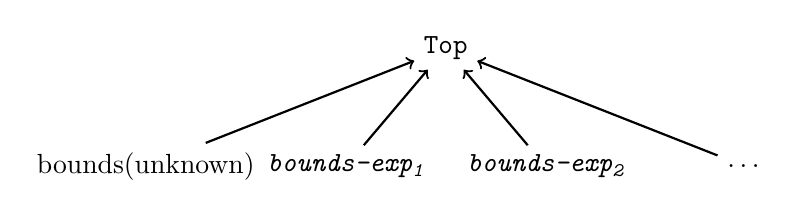
\begin{tikzpicture}[sibling distance=1in]
\node[rectangle, minimum size=8pt]{\texttt{Top}}
  child foreach \name in {\boundsunknown, \var{bounds-exp\textsubscript{1}},
                          \var{bounds-exp\textsubscript{2}}, \ldots}
     {node{\name} edge from parent[<-, thick]};
\end{tikzpicture}
\end{center}
\caption{The lattice of values used in dataflow computation of extent}
\label{fig:extent-dataflow-lattice}
\end{figure}

For an assignment to an \arrayptr\ variable, the existing
lattice value for the \arrayptr\ variable is killed, unless
the special conditions described in Section~\ref{section:extent-of-declarations}
are met.
A new lattice value is generated for the \arrayptr\ variable. If the
assignment declares bounds for the \arrayptr\ variable, the new
lattice value is the bounds expression in the bounds declaration.
Otherwise, it is the value \boundsunknown.

A declaration of a variable is handled similarly to an assignment,
except that there will not be any lattice value to kill. Lexical hiding
of variables involved in bounds declarations is not permitted. If the
declaration declares bounds for the \arrayptr\ variable, the
new lattice value is the bounds expression in the bounds declaration.
Otherwise, it is the value \boundsunknown.

A variable going out of scope kills any existing lattice values in which
that variable occurs.

At control-flow split points, the lattice values for the
\arrayptr\ variables flow to all branches of the split. The
propagation is dataflow-sensitive but not control-flow sensitive. At
control-flow join points, the lattice values are unioned (moving upward
in the lattice). If the lattice values for an \arrayptr\
variable are not the same, the resulting value is \texttt{Top}.

\section{Bounds declarations and loops}

Loops often operate on variables declared outside of loops. They may
read the variables and then update the variables. When these variables
are \arrayptr\ variables they must have bounds and the bound
must be loop invariants.

The common case is that the bounds expression is invariant across all
iterations of the loop. The earlier \code{sum} example illustrates
this. The variable \code{current} is declared with bounds before a
loop. The loop modifies \code{current}, but the bounds for
\code{current} do not change:

\begin{lstlisting}
/* sum integers stored between start and end, where end is not included */
int sum(array_ptr<int> start where start : bounds(start, end), array_ptr<int> end)
{
    int sum = 0;
    array_ptr<int> current : (start, end) = start;

    while (current < end) {
       sum = *current;
       current += 1; // bounds do not need to be redeclared here.
    }
}
\end{lstlisting}

A programmer can declare bounds expressions that change on each
iteration of the loop. This may be necessary if an \arrayptr\
variable is modified to point to different memory during a loop
iteration. It also may be desirable for performance reasons. In either
case, there needs to be a loop-invariant bounds declaration.

The following example illustrates this. It is an implementation of
lexicographic comparisons of two arrays, using one pointer to scan each
array. The bounds at the variable declarations serve as loop invariant
bounds. The lower bounds for a variable are declared using the variable
itself, to reduce register pressure in the loop. This can enable
compilers to generate better code. Note that an optimizing compiler will
eliminate the runtime bounds checks easily.

\begin{lstlisting}
/* lexicographic comparison of two arrays of integers */
int compare(array_ptr<int> x : bounds(x, x_end),
            array_ptr<int> y : bounds(y, y_end)
            array_ptr<int> x_end, array_ptr<int> y_end)
{
  while (x < x_end && y < y_end) {
    if (*x == *y) { // bounds check: x >= x && x < x_end; easily
                    // optimizable.
                    // bounds check: y >= y && y < y_end; easily
                    // optimizable.
      x++;
      y++;
    }
    else if (*x < *y) { // bounds checks here are easily optimizable too.
      return -1;
    }
    else {
      return 1;
    }
  }
  if (x == x_end && y == y_end) {
    return 0;
  }
  else if (x != x_end) {
    return 1;
  }
  else {
    return -1;
  }
}
\end{lstlisting}


% !Tex root = checkedc.tex

\chapter{Bounds for expressions and bounds declaration checking}
\label{chapter:checking-bounds}

The prior chapter described how to declare bounds for variables.
This chapter describes how to infer a bounds expression for 
an expression, starting from the declared bounds for variables.
An inferred bounds expression
describes the range of memory that can be accessed (if any) using 
the values produced by expression.  Inferred bounds expressions
are used in runtime bounds checks.   This chapter also describes how to
 check that declared bounds for variables are valid at initialization
 time and after assignments.

Bounds expressions for expressions are inferred using inference
rules.  The inference rules are defined by induction over expressions, 
the same way that typechecking rules work.  Given an expression
and bounds expressions for its subexpressions, a bounds expression
is constructed.  The induction base cases are variables (for which
bounds expressions are declared by the programmer) and constants.
The inference may require the compiler to introduce temporaries to
hold the values of subexpressions.

Bounds declarations are invariants about program variables
that must be checked at compile time.  The key idea is {\em subsumption checking}.
At \arrayptr\ variable declarations and assignments, 
the right-hand side expression must have a bounds expression that includes (subsumes) 
the declared bounds  expression for the variable.  The memory that is accessible using
the right-hand side must include all the memory that is accessible via the variable.
In addition, after assignments to variables used in declared bounds, the
declared bounds must still be valid.

Subsumption checking is parameterized by {\it sets of equivalent non-modifying expressions}.
Two non-modifying expressions are equivalent if they
evaluate to the same value given the program state at the program point where 
checking is being done.  Assignments create equivalent non-modifying
expressions. Equivalence can also be inferred by dataflow analysis.

To handle both assignments to pointer variables with bounds and assignments
to variables used in bounds, we generalize bounds declaration
checking to operate over {\em contexts}.  Contexts are maps from variables
to bounds expressions for the values stored in the variables.
For each {\em full expression} in a function, we start with a context based
on declared bounds.
A full expression \cite[Annex C]{ISO2011} is an expression not nested within another expression.
We analyze the full expression and produce a new
context that describes the bounds for variables after assignments
in the expression have been completed.  We then check that the bounds
expressions in the context subsume the declared bounds for variables.

The analysis of expressions is complicated by C's evaluation
rules for expressions.  C does not have a precise order of evaluation
for expressions.  The times at which assignments
must happen within expressions are only partially constrained.
C also allows control flow within 
expressions via comma expressions, conditional expressions, and
logical boolean expressions (the \code{&&} and \code{\|\|} expressions).

To handle this, the analysis tracks sets of variables where assignments
to those variables may not have been completed yet.  We call these
variables {\em pending variables} and the sets of variables {\em
pending sets}.  When the order of evaluation of expressions
is indeterminate, variables are added to pending sets.
The analysis tracks the flow of information through expressions, relying on the
pending sets to prevent undefined uses of variables or conflicting
assignments to variables.  We disallow some complicated expressions
that combine conditional assignments and unordered assignments
to variables used in the same bounds declaration.

The descriptions of bounds inference and bounds checking are
presented in a cumulative fashion.  We start with the simplest
analysis, bounds inference for expressions.  We then extend that
with progressively more complicated analyses.
Section~\ref{section:inferring-expression-bounds}
describes how to determine the bounds for an expression of type \arrayptr.
It does not cover operations that access data structures, such as member
access and pointer dereference. 
Those are covered in Chapters~\ref{chapter:structure-bounds} and 
\ref{chapter:pointers-to-data-with-arrayptrs}.
Section~\ref{section:checking-simple-assignment} describes
how to check bounds declarations for a simple assignment
expression.
Section~\ref{section:checking-complex-expressions}
extends this to cover more complex cases where there is control-flow
or multiple assignments within an expression.

Section~\ref{section:checking-full-expressions} describes
subsumption checking on bounds expressions.   The subsumption checking
puts expressions into a standard form.  It then uses syntactic equality,
extended with simple identities about C expressions and taking into account expression
equivalence information.
Inference steps for relational reasoning about bounds expressions 
are described in Chapter~\ref{chapter:simple-invariants}.

Section~\ref{section:checking-function-call-arguments}
describes validating function call arguments.

\section{Preparing a translation unit for checking}

To simplify the rules for checking, some syntactic transformations are done
on a translation unit before checking.  First, some syntactic cases are
replaced with semantically-equivalent cases.  This reduces the number of cases
that must be covered by the checking rules.  In-line return bounds expressions
are replaced with the form that uses a name for the return value. The form
\boundsdecl{\var{f}(\ldots{})}{\var{e1}} is changed to 
\texttt{\var{f}(\ldots{}) \keyword{where}
  \boundsdecl{\code{return_value}}{e1}}.
The \code{count} and
\code{byte_count} bounds expressions are also expanded to bounds expressions.
The form \boundsdecl{\var{x}}{\boundscount{\var{e1}}}
is replaced with \boundsdecl{\var{x}}{\bounds{\var{x}}{\var{x} \code{+} \var{e1}}}
and \boundsdecl{\var{x}}{\boundsbytecount{\var{e1}}}
is replaced with \boundsdecl{\var{x}}{\bounds{\cast{\arrayptrchar}{\var{x}}}
                                             {\cast{\arrayptrchar}{\var{x} \lstinline|+| \var{e1}}}}.
For now, we ignore the additional side conditions on count expressions. Checking of these
conditions will be addressed in Chapter~\ref{chapter:simple-invariants}.

Also, relative alignment is made explicit for all bounds
declarations: \boundsdecl{\var{x}}{\bounds{\var{e2}}{\var{e3}}} is expanded to
\boundsdecl{\var{x}}{\boundsrelval{\var{e2}}{\var{e3}}
                                  {\sizeof{\lstinline|typeof(|\var{x}\lstinline|)|}}}.
For code without explicit or implicit casts of \arrayptr s, relative
alignment can be ignored.

In the checking rules, sometimes shorter syntactic forms are used for
brevity. The shorter forms should be replaced with their full forms before
using the rules.

Second, lexical hiding of variables is eliminated by renaming variables so that
hiding no longer happens\footnote{Note that compilers typically do not need to
rename variables. Compilers already disambiguate variables with the
same name and the disambiguation mechanisms can be used in the implementation
of the checking rules.  For example, some compilers use distinct objects
to represent each variable declaration.}.  If a variable with block scope that does not
have external linkage has the same name as a variable with file scope or
a variable with an enclosing block scope, the variable
should be renamed to be distinct from other variables.  Similarly, parameter
variables that have the same name as a variable with file scope or a
variable with an enclosing block scope should be renamed.

\section{Inferring bounds expressions for expressions}
\label{section:inferring-expression-bounds}

We first discuss inferring bounds expressions for expressions. The bounds for an
expression are always determined with respect to a bounds
declaration context, which maps variables to their
bounds expressions.  We will use $\vdash$ to denote the
valid bounds for an expression. The notation \boundsinfer{\var{e}}{\var{bounds-exp}}
means that expression \var{e} has valid bounds \var{bounds-exp}.

At times, we need to discuss bounds that are given in terms of the value
of an expression or a subexpression.   For example, a function call expression may
return an \arrayptr\ pointer to an array of constant size
\var{n}. The bounds for that pointer value would be (the
\arrayptr\ pointer, the \arrayptr\ pointer +
\var{n}). We use temporaries to denote the values
of expressions or subexpressions.   A temporary is a compiler-introduced
temporary variable that is initialized immediately upon evaluation of an
expression.   It differs from a source-level variable, whose assignment
may happen at some less-precisely specified time.   The evaluation of
expressions at runtime needs to store values in a temporary, 
if the temporary is used in a runtime
bounds check.

\subsection{Null pointers}

The bounds for 0 is the \lstinline|any| bounds:

\boundsinfer{0}{\boundsany}

\subsection{Variables}
\label{section:checking-variables}

Suppose there is a use of some variable \var{x}.

\begin{itemize}
\item
  If \var{x} has type \arrayptr, the bounds are the result of
  the analysis in Section~\ref{section:extent-definition}
  for this occurrence of \var{x}.
\item
  If \var{x} has type \ptrT, 
  \boundsinfer{\var{x}}{\boundsrel{\var{x}}{\var{x} \code{+ 1}}{\var{T}}}.
   On the right-hand side, \var{x} is reinterpreted as having \arrayptr\ type.
\item
  If \var{x} has an array type, the rules depend on whether \var{x}  is a parameter
  variable.  Typechecking in C treats a parameter variable with the type ``array of \var{T}''
   as though it has the type ``pointer to \var{T}''.   It does not enforce 
  at function calls that actual arguments have the required dimension size.  This means
  that the declared outermost bounds cannot be trusted for parameters with unchecked
  array types.  In contrast, local variables and externally-scoped variables are allocated 
  space for their declared types.  Declared dimension information for them can be trusted 
  regardless of whether they have checked or unchecked array types.  Checking of bounds 
  declarations for checked arrays  enforces that actual arguments meet the required
  dimension size.
\begin{itemize}
\item If 
\begin{itemize} 
\item \var{x} is a local variable or an externally scoped variable 
\item or \var{x} is a parameter variable with a checked array type
\end{itemize}
and \var{x} has a known number of elements \var{n}, then  
  \boundsinfer{\var{x}}{\boundscount{\var{n}}}.
\item Otherwise, the bounds are the result of the analysis in 
  Section~\ref{section:extent-definition} for this occurrence of \var{x}.
\end{itemize}
\item  Otherwise \var{x} has \boundsunknown.
\end{itemize}

\subsection{String literals and compound literal expressions}
A string literal \lstinline+''abc''+ evaluates to an lvalue with array type,
as does a compound literal of the form \lstinline+(int []) { 0, 1, 2, 3}+.
These lvalues are then converted implicitly to values with pointer type.

During bounds checking, a temporary is introduced for the result
of evaluating a string literal or compound literal expression.
If a literal \var{e} has array type and \var{n} elements, the bounds
exclude the null terminator, if there is one.
\begin{itemize}
\item If $e$ is a string literal or a compound literal expression with
a null-terminated array type,
\boundsinfer{\var{e}}{\bounds{temporary for \var{e}}{temporary for \var{e} + (\var{n - 1})}}.
\item Otherwise,
\boundsinfer{\var{e}}{\bounds{temporary for \var{e}}{temporary for \var{e} + \var{n}}}
\end{itemize}

\subsection{Address-of expressions}
\label{section:address-of-expression-bounds}

There are three kinds of address-of expressions:
\begin{itemize}
\item Address of a variable (\lstinline|&|\var{x}): a variable \var{x} with type \var{T} 
whose address is taken is considered to be an array of one element:

\boundsinfer{\lstinline|&|\var{x}}
            {\boundsrel{\lstinline|&|\var{x}}{\lstinline|&|\var{x} \lstinline| + 1|}{\var{T}}}.
            
\item Address of a pointer dereference operation (\lstinline|&*|\var{e}):
The address-of operation and the pointer dereference operation cancel. 
The bounds are the bounds of the underlying expression. 
If \boundsinfer{\var{e}}{\var{bounds-exp}}, then
\boundsinfer{\lstinline|&*|\var{e}}{\var{bounds-exp}}.

\item Address-of a subscripting expression (\lstinline|&|\var{e1}\lstinline|[|\var{e2}\lstinline|]|):
This is the same as taking the address of a pointer dereference operation.
According to the C semantics, \var{e1}\lstinline|[|\var{e2}\lstinline|]| is equivalent
to \lstinline|*(|\var{e1} \lstinline|+| \var{e2}\lstinline|)|.  If 
\boundsinfer{\var{e1} \lstinline|+| \var{e2}}{\var{bounds-exp}}, then
\boundsinfer{\lstinline|&|\var{e1}\lstinline|[|\var{e2}\lstinline|]|}{\var{bounds-exp}}.
\end{itemize}
   
\subsection{Function calls}
\label{section:inferring-bounds-for-function-calls}

Let \var{f} be the name of a function that returns an
\arrayptr\ value (pointers to functions will be handled later).
Suppose there is a function call expression of the form
\var{f}\code{(}\var{e1 \ldots{} en}\code{)}:

\begin{enumerate}
\item
  If \var{f} has a bounds declaration for the return value of the form
  \code{return_value :} \var{exp1}, then

  \begin{itemize}
  \item
    Any arguments that correspond to formal parameters occurring in
    \var{exp1} must be valid non-modifying expressions. If they are
    not, \boundsinfer{\var{f}\lstinline|(|\var{e1} \ldots{} \var{en}\lstinline|)|}{\boundsunknown}.
  \item
    Otherwise, substitute \var{e1} \ldots{} \var{en} for the formal
    parameters of \var{f} occurring in \var{exp1}. Also substitute the
    special symbol \exprcurrentvalue\ for
    \code{return_value}. These substitutions produce \var{exp2}.
    \boundsinfer{\var{f}\lstinline|(|\var{e1} \ldots{} \var{en}\lstinline|)|}{\var{exp2}}.
  \end{itemize}
\item
  If \var{f} does not have a bounds declaration for its return value,
  then \boundsinfer{\var{f}\lstinline|(|\var{e1} \ldots{} \var{en}\lstinline|)|}{\boundsunknown}.
\end{enumerate}

The special variable \lstinline|return_value| may appear in \var{exp1}. It
is the value of the function call expression. If \lstinline|return_value|
is used, a temporary variable is introduced to hold the result of the
function call.  The occurrences of \lstinline|return_value| are replaced
with the the temporary variable.

There needs to be validation that the bounds for argument expressions
match the required bounds for formal parameters. This is described in
Section~\ref{section:checking-function-call-arguments}.

The following code provides examples of function call expressions where
bounds need to be computed. In the code, the programmer wraps a call to
\code{malloc} in an allocation helper, \code{alloc_helper}. The
function \code{alloc_helper} returns an \arrayptr\ value
that is passed as an argument to \code{init}, which initializes the array
and returns the \arrayptr\ value.
\begin{lstlisting}
array_ptr<int> alloc_helper(int n) : count(n)
{
    array_ptr<int> result : count(n) = malloc((sizeof(int) * n);
    return result;
}

array_ptr<int> init(array_ptr<int> target : count(s), 
                    int s) : count(s)
{
    for (int i = 0; i < count; i++) {
         target[i] = i;
    }

    return target;
}

void go(int size) 
{
    array_ptr<int> x : count(size) = init(alloc_helper(size), size);
    ...
}
\end{lstlisting}

First, syntactic forms for bounds expressions are expanded to eliminate
count expressions and in-line return expressions, as well as make
relative alignment explicit.

\begin{lstlisting}
array_ptr<int> alloc_helper(int n)
where return_value : bounds(return_value, return_value + n) rel_align(int)
{
    array_ptr<int> result : bounds(result, result + n) rel_align(int) =
      malloc((sizeof(int) * n);
    return result;
}

array_ptr<int> init(array_ptr<int> target : bounds(target, target + s)
                                            rel_align(int), 
                    int s) 
where return_value : bounds(return_value, return_value + s) rel_align(int)
{
    for (int i = 0; i < count; i++) {
      target[i] = i;
    }

    return target;
}

void go(int size) 
{
    array_ptr<int> x : bounds(x, x + size) rel_align(int) = 
        init(alloc_helper(size), size);
    ...
}
\end{lstlisting}

The valid bounds for the call to \lstinline|init(alloc_helper(size),size)| in
\lstinline|go| are computed using the return bounds for \lstinline|init|:

\begin{lstlisting}
    return_value : bounds(return_value, return_value + s) rel_align(int)
\end{lstlisting}

First, there is a check that all the actual arguments corresponding to
the formal parameters used by the return bounds expression are valid
non-modifying bounds expressions. This check succeeds even though the
first actual argument \lstinline|alloc_helper(size)| is not a valid bounds
expression. The formal parameter \lstinline|target| is not used by the
return bounds expression.

Next, the actual arguments are substituted for the formal parameters and
a new temporary \var{t1} is substituted for \lstinline|return_value|.
(\var{t1} is distinct from source-level variables).
The argument \lstinline|size| is substituted for \lstinline|s|, producing
\begin{lstlisting}[escapechar=\|]
    init(alloc_helper(size), size) |\(\vdash\)| bounds(|\var{t1}|, |\var{t1}| + size) rel_align(int)
\end{lstlisting}

% TODO: we can now introduce a temporary for the result of the function call, so this
% is confusing given the discussion below for alloc_helper, where we do that.
%   Checking of call arguments would fail due to the potential inequality
% of two function call expressions.  These issues should be explained in checking of function arguments.
%
%It would not be possible to represent the bounds if \lstinline|size| were a
%function call too:
%\begin{lstlisting}
%    array_ptr<int> x = init(alloc_helper(getsize()), getsize());
%\end{lstlisting}
%
%Function calls are not valid in bounds expressions:
%
%\begin{lstlisting}[escapechar=\|]
%   bounds(|\var{t1}|, |\var{t1}| + getsize())  // illegal
%\end{lstlisting}
%
%The solution would be to assign the result of \lstinline|getsize()| to a
%variable:
%\begin{lstlisting}
%   int tmp = getsize();
%   array_ptr<int> x = init(alloc_helper(tmp), tmp);
%\end{lstlisting}

The parameters to the call to \lstinline|init| need to be validated
(see Section~\ref{section:checking-function-call-arguments}). This
requires determining the valid bounds for \lstinline|alloc_helper(size)|. The
return bounds for \lstinline|alloc_helper| are used:
\begin{lstlisting}
   return_value : bounds(return_value, return_value + n) rel_align(int)
\end{lstlisting}

First, there is a check that the actual arguments that correspond to
formal parameters used in the return bounds are valid non-modifying
expressions. The only argument is the variable size, so this check
succeeds. Next, \lstinline|size| is substituted for \lstinline|n| and
a new temporary variable \var{t2} is substituted for \lstinline|return_value|, producing:
\begin{lstlisting}[escapechar=\|]
   alloc_helper(size) |\(\vdash\)| bounds(|\var{t2}|, |\var{t2}| + size) rel_align(int)
\end{lstlisting}

\subsection{Pointer arithmetic}

The range of memory accessible through pointer arithmetic expressions
remains unchanged from the underlying pointer. In other words, for
\boundsinfer{\var{x}}{\var{bounds-exp}}, the bounds expression for any
pointer arithmetic involving \var{x} is the same as the one for
\var{x}. This is because that C semantics for pointer arithmetic is
that if \var{x} points to an object at runtime, any pointer arithmetic
involving \var{x} must produce a pointer to the same object. The bounds
of the object in memory are not changed by the pointer arithmetic.

We first cover the typical situation where the relative alignment type
for a pointer in a pointer operation matches the referent type of the
pointer. Given a pointer operation of the form \var{x op e1}, where \var{x}
has an \arrayptr\ type, \var{e1} has an integral type, and
\var{op} is addition or subtraction, the memory that can be accessed
through \var{x op e1} is the same memory that can be accessed through
\var{x}:

\begin{itemize}
\item
  If \var{x} is a pointer to \var{T} and 
  \boundsinfer{\var{x}}{\boundsrel{\var{e2}}{\var{e3}}{\var{T}}},
  then \boundsinfer{\var{x} \var{op} \var{e1}}{\boundsrel{\var{e2}}{\var{e3}}{\var{T}}}.
\end{itemize}

This can be extended to pointer operations of the form \var{e4 op e1},
where \var{e4} has type
\arrayptrT\ as
follows:

\begin{itemize}
\item
  If \var{e4} is a pointer to \var{T} and 
  \boundsinfer{\var{e4}}{\boundsrel{\var{e2}}{\var{e3}}{\var{T}}}
  then \boundsinfer{\var{e4 op e1}}{\boundsrel{\var{e2}}{\var{e3}}{\var{T}}}
\end{itemize}

Here is the full rule that handles the situation where the relative
alignment of the pointer differs from the size of the referent type of
the pointer. GCD computes the greatest common divisor of two integers.
The prior rules are just special cases of this rule:

\begin{quote}
If \var{e4} is a pointer to \var{T} and 
\boundsinfer{\var{e4}}
            {\boundsrel{\var{e2}}
                       {\var{e3}}
                       {\var{c}}}
then \boundsinfer{\var{e4 op e1}}
                 {\boundsrel{\var{e2}}
                            {\var{e3}}
                            {\texttt{GCD(\var{c}, \sizeof{\var{T}})}}}.
\end{quote}

\subsubsection{Pointer arithmetic for unchecked pointer types}

Pointer arithmetic involving an \arrayptr\ value checks that
the value is non-null and generates a runtime error if it is. This check
is important because a null pointer may have invalid bounds (this
follows from the definition of the meaning of bounds in 
Section~\ref{section:bounds-declarations}). It
prevents a null pointer that has invalid bounds from being used to create a
non-null pointer with valid bounds, which could then be used to access
memory.

Because the meaning of unchecked pointers has not changed, pointer
arithmetic involving a null unchecked pointer may not generate a runtime
error. The rules for array\_ptr pointer arithmetic can be applied to
unchecked pointer arithmetic, however, provided that a side condition that
the pointer expression is non-null is added:

\begin{quote}
If \var{e4} is a pointer to \var{T} and it can be proved that
\var{e4} \code{!= 0} and 
\boundsinfer{\var{e4}}{\boundsrel{\var{e2}}{\var{e3}}}{\var{c}}, then
\boundsinfer{\var{e4 op e1}}{\boundsrel{\var{e2}}{\var{e3}}
                                            {\texttt{GCD(\var{c},\sizeof{\var{T}})}}}.
\end{quote}

Chapter~\ref{chapter:simple-invariants}
provides a general framework for checking side-conditions as
part of checking bounds declarations.

\subsection{Cast expressions}
\label{section:cast-expressions}

Given a cast expression of the form \cast{\var{T}}{\var{e}},
the bounds for \var{e} are determined. The bounds for
\var{e} are used as the bounds for the entire expression.
  
\subsection{Conditional expressions}

Given an expression of the form \var{e1} \code{?} \var{e2}
\code{:} \var{e3}, the bounds for \var{e2} and \var{e3} are
determined. They must be syntactically identical (after putting the
bounds into a normal form). The bounds for \var{e2} are used as the
bounds for the entire expression.

\emph{This is an expression where a conditional bounds expression could
be used to represent the resulting range.  Another alternative that works
with current syntax would be to create upper/lower-bound expressions
that use e1 such as (e1 ? lower-bound(e2) : lower-bound(e3), e1 ?
upper-bound(e2) : upper-bound(e3). For now, we defer discussion of both
alternatives. }

\subsection{Comma expressions}

Given an expression of the form \var{e1} \code{,} \var{e2}, the
bounds for \var{e2} are determined. The bounds for \var{e2} are used
as the bounds for the entire expression.  

\subsection{Assignment expressions}

Given an expression of the form \var{e1} \code{ = } \var{e2}, the
bounds for \var{e2} are determined. The bounds for \var{e2} are used
as the bounds for the entire expression.

Note that if \var{e1} is a variable,
there is an order of evaluation issue if \var{e1} appears in the bounds for
\var{e2}.   Specifically, the bounds for \var{e2} cannot be used to
check a memory access within the full expression being evaluated.

\subsection{Pre-and-post increment operators}
\label{section:inferring-increment-bounds}

Given an expression of the form \code{++}\var{e1}, \code{--}\var{e1},
 \var{e1}\code{++} or \var{e1}\code{--}, where $e1$ has a pointer type,
 the bounds for $e1$ are the bounds for the entire expression.
 
 If $e1$ appears in its own bounds, the compiler should introduce a
 temporary to hold the value of $e1$ before the update, and use
 the temporary in the bounds.  In the case of post-increment operators, 
 the C semantics already require  introducing a temporary for the value of $e1$.

\section{Bounds declaration checking for simple assignments}
\label{section:checking-simple-assignment}

This section describes how to check bounds declarations for
simple assignments to variables.  These are expression statements of the
form \code{v = e1}, where \code{v} is a variable and \code{e1} does
not contain nested assignments.
Section~\ref{section:checking-complex-expressions} handles nested assigments.

Given an expression of the form \var{v}\lstinline+=+\var{e}, the effect of the assignment
to \var{v} is modelled by updating the context to contain bound expressions that are true
after the assignment.  If \var{v} has \arrayptr\ type, the bounds expression in
the context for \var{v} is updated to the inferred bounds expression for \var{e}.
We also model the change in \var{v}'s
value for any bounds expressions in the context that use \var{v}.   If the result of 
evaluating \var{e} is available in a temporary, we update the sets of equivalent
expressions to record that \var{v} equals the temporary when the (top-level) assignment
expression is completely evaluated.
We use the updated context and sets of equivalent expressions to check
that the new bounds expressions subsume the declared bounds expressions for variables.

For an assignment expression of the form \var{x} \code{=} \var{e},
where \var{x} is a variable and \var{e} is an expression, there are
three aspects to to computing bounds. 
\begin{itemize}
\item Infer the bounds expression for \var{e}.
\item Determine the effect of the assignment on the
bounds declaration context.
We start with the context that is true before the expression
is evaluated and determine the context that is true after
the expression is evaluated.
\item If the value of \var{e} is also available in a temporary,
we record in the expression equivalence set that \var{x} equals that
temporary (at the end of evaluating the expression).
\end{itemize}
It seems straightforward to determine the effect of the assignment
on the context.   If \var{x} has type
\arrayptr, use the computed bounds for \var{e} to update the context
so that the bounds for \var{x} are the bounds of \var{e}.
However, there is a problem. The bounds for \var{e} is determined
\var{before} \var{x} changes value. When \var{x} changes value, the bounds
for \var{e} may no longer be true if \var{x} appears in the bounds.
The context could contain uses of \var{x} also in bounds expressions.

A simple solution is to invalidate bounds expressions where \var{x} appears in
the bounds. This does not work well when a variable that appears in its
own bounds declaration is incremented or decremented. Consider the
following example:
\begin{lstlisting}
array_ptr<int> x : bounds(x, high) = ...
int sum = 0;
while (x < high) {
    sum += *x;
    x++;  // bounds for x would be undefined for the simple solution
}
\end{lstlisting}

A possible solution is to require programmers to copy variables in loops
that are modified using only pointer arithmetic to temporary variables
before the loop. The temporary variables could then be used in bounds.
However, this might increase register pressure and worsen performance.

One can do better than that for loop induction variables, which are
variables that are incremented or decremented by a constant in a loop.
Condit \textit{et al.} observe that some assignment expressions are
invertible: the old value of a variable can be calculated from the new
value . One can update the bounds by substituting the inverted
expression in place of the variable. The updated bounds can then be
narrowed to satisfy loop bounds invariants. Invertible expressions
include the addition and subtraction expressions that update loop
induction variables.

The updated context is determined in two steps. First, if
\var{x} has type \arrayptr, the context is updated for
\var{x} using bounds expressions that use the \emph{old} value of \var{x}:

\begin{enumerate}
\item
  If \boundsinfer{\var{e}}{\var{exp}}, then the context is updated with
  \boundsdecl{\var{x}}{\var{exp}}.
\item
  Otherwise, the context is updated with \boundsdecl{\var{x}}{\boundsunknown}
   to indicate that \var{x} has no valid bounds.
\end{enumerate}

Second, the context is updated to reflect the change in the value of
\var{x}:

\begin{itemize}
\item
  If the expression being assigned is invertible, the right-hand side of
  any bounds expression that uses \var{x} will be updated to use an
  expression that inverts the new value to compute the old value.
\item
  Otherwise, any bounds expression that involves \var{x} is invalidated
\end{itemize}

\subsection{Invertibility}

The following examples illustrate invertibility and updating bounds. For
the first example, suppose there is a declaration of an
\arrayptr\ variable followed by a decrement of a variable
involved in the bounds:

\begin{lstlisting}
array_ptr<int> a : count(len) = ...
len = len - 1
\end{lstlisting}

The original value of \lstinline|len| can be computed from the new value.
In this case, a valid new bounds after the decrement of \lstinline|len| is
\lstinline|count(a)  == len + 1.| The bounds for \lstinline|a| after the
assignment are:
\begin{lstlisting}
len = len - 1
where a : count(len + 1);
\end{lstlisting}

For the second example, consider an update to a pointer variable that
appears in its own bounds:
\begin{lstlisting}
array_ptr<int> p : bounds(p, high) = ...         
while (p < high) {
    ...
          p = p + 1;
}
\end{lstlisting}

First, the new bounds expression for the expression \lstinline|p + 1| is
computed. It is the same as the original bounds expression
\lstinline|bounds(p, high)|. Because \code{p} is modified by the assignment, the
inverted expression for \lstinline|p + 1| is substituted into
\lstinline|(p, high)|. The inverted expression for \lstinline|p + 1| is \lstinline|p - 1|.
This leads to bounds of the form \lstinline|bounds(p - 1, high)|:

\begin{lstlisting}
while (p < high) {
    ...
          p = p + 1 where p : bounds(p - 1, high);
}
\end{lstlisting}

Bounds validity is preserved when the range of a bounds expression is
narrowed. \lstinline|(p - 1, high)| implies that \lstinline|(p, high)| is a
valid bounds expression. This reestablishes the loop bounds invariant
for \lstinline|p| of \lstinline|(p, high)|.

\begin{lstlisting}
while (p < high) {
    ...
          p = p + 1 where p : bounds(p, high);
}
\end{lstlisting}

The correctness of narrowing depends on pointer arithmetic overflow
for checked pointer types being a runtime error. For a lower bound \var{e1} in a bounds
expression, we can only substitute \var{e2} for \var{e1} as the lower
bound if \var{e2} \code{>=} \var{e1}. The identity \code{p > p - 1} 
holds only if overflow is a runtime error.

\subsection{Invertible expressions}
An expression is invertible with respect to a variable \var{x} if:

\begin{enumerate}
\item
  The expression is \var{x}
\item
  or

  \begin{enumerate}
  \item
    The operator in the expression is an addition, subtraction, one's
    complement, unary minus, unary plus, exclusive-or, a bit-preserving
    cast operator, or a widening cast operator, and
  \item
    The variable \var{x} occurs only in one argument of the operation and that
    argument is an invertible expression with respect to \var{x}, and
  \item

    Any other argument of the operation is a non-modifying expression,
    excluding non-modifying expressions that are or include member
    references, indirect member references, or pointer dereferences.
  \end{enumerate}
\end{enumerate}

The addition and subtraction operations must be for checked pointer
arithmetic or unsigned integer arithmetic. An implementation may allow
integral addition and subtraction operations to be invertible if
integral addition and subtraction are defined as two's complement
arithmetic where extra bits are discarded on overflow. However, this
introduces the possibility of non-portable code.

Given the expression \var{x} \code{=} \var{e}, where \var{x} occurs once
in \var{e}, mathematical rules are applied to solve for \var{x} in
\var{e}. We generalize the left-hand side from \var{x} to an expression
\var{f} and define \texttt{inverse(}\var{f}\texttt{,}
\var{e}\texttt{)} as follows:

\begin{longtable}[c]{@{}ll@{}}
\toprule
Given \texttt{inverse(\var{f}, \var{e})}, where & the result is:\tabularnewline
\midrule
\endhead
\var{e} = \texttt{x} & \var{f}\tabularnewline
\var{e} = \code{\~}\var{e1} &
\texttt{inverse(\code{\~}\var{f}, \var{e1})}\tabularnewline
\var{e} = \code{-}\var{e1} & \texttt{inverse(\code{-}\var{f}, \var{e1})}\tabularnewline
\var{e} = \code{+}\var{e1} & \texttt{inverse(\code{+}\var{f}, \var{e1})}\tabularnewline
\var{e} = \cast{\var{t1}}{\var{e1}}, where \var{e1} has
type \var{t2} & \texttt{inverse(\cast{\var{t2}}{\var{f}},
\var{e1})}\tabularnewline
and \code{(}\var{t1}\code{)} is not a narrowing cast & \\
\var{e} = \var{e1} \code{+} \var{e2}, where \texttt{x} occurs in
\var{e1} & \texttt{inverse(}\var{f} \code{-} \var{e2},
e1)\tabularnewline
\var{e} = \var{e1} \code{+} \var{e2}, where \texttt{x} occurs in
\var{e2} & \texttt{inverse(}\var{f} \code{-} \var{e1},
\var{e2})\tabularnewline
\var{e} = \var{e1} \code{-} \var{e2}, where \texttt{x} occurs in
\var{e1} & \texttt{inverse(}\var{f} \code{+} \var{e2},
\var{e1})\tabularnewline
\var{e} = \var{e1} \code{-} \var{e2}, where \texttt{x} occurs in
\var{e2} & \texttt{inverse(}\var{e1} \code{-} \var{f},
\var{e2})\tabularnewline
&\tabularnewline
\var{e} = \var{e1} \code{^} \var{e2}, where \texttt{x} occurs in
\var{e1} & \texttt{inverse(}\var{f} \code{^} \var{e2},
\var{e1})\tabularnewline
\var{e} = \var{e1} \code{^} \var{e2}, where \texttt{x} occurs in
\var{e2} & \texttt{inverse(}\var{f} \code{^} \var{e1},
\var{e2})\tabularnewline
\bottomrule
\end{longtable}

Given \texttt{inverse(x}, \var{e}), the rules are applied repeatedly
until the original value of x in e has been computed. Here is an example
of computing the inverse of \code{x = (x + 4) + 5}:
\begin{lstlisting}
   inverse(x, (x + 4) + 5) =
       inverse(x - 5, x + 4) =
          inverse((x - 5) - 4, x) =
              (x - 5) - 4
\end{lstlisting}

\section{Bounds declaration checking for expressions}

\label{section:checking-complex-expressions}

This section generalizes bounds declaration checking for a single
assignment expression to expressions with control-flow or multiple
assignments.
It builds on the bottom-up analysis in
Section~\ref{section:inferring-expression-bounds}.

\subsection{Order of evaluation and checking}
\label{section:avoiding-undefinedness}

The order of evaluation of side-effects in subexpressions of an expression is defined in C only for 
control-flow expressions and in certain other circumstances \cite[Section 6.5,Annex C]{ISO2011}).
Otherwise, the order of evaluation of side-effects is undefined.   This complicates checking 
because an expression with an undefined order of evaluation of side-effects might have an 
undefined meaning.  Checking must produce an error for these expressions because the
validity of bounds information is not maintained by such expressions. In addition, checking must still
model the order of side-effects when the order is defined.

The meaning of an expression is undefined if:

\begin{enumerate}
\item
  There are multiple assignments to the same variable within an
  expression where the order of evaluation of the assignments is
  undefined, or
\item
  There is an assignment to a variable that is also used by the
  expression, where the order of evaluation of the assignment and the
  use is undefined.
\end{enumerate}

The following statements illustrate these problems:

\begin{lstlisting}
y = (x = 5) + (x = 6);
i = i++ + 1;
a[i++] = i;
\end{lstlisting}


In the first case, the value of the right-hand side expression is 11,
yet at the end of the expression, the value of x could be 5 or 6. In the
second case, there are two assignments to i and the order is undefined.
In the third case, it is not clear when i is read versus when it is
modified.

Note that a C compiler may choose an order of evaluation and
define the meaning of an expression anyway.  We still
require that a compiler produce an error when checking
bounds declarations for expressions with undefined meaning
according to the definition just given.  This ensures that the checking
is the same across compilers.

Bounds checks can lead to a subtle version of an unordered assignment
and use.  An expression may have an assignment through a pointer that requires a
bounds check. The bounds for the pointer expression may include a
variable that is modified in the expression, where the order of
evaluation of the assignment through the pointer and the variable
assignment is undefined. This means that the order of evaluation of the
bounds check and the variable assignment is undefined.

This example illustrates this problem:

\begin{lstlisting}
w = ...
where w : bounds(x, x + y);
int t = *w + (y = tmp);
\end{lstlisting}

The variable y is an integer variable that is a count of elements. It is
overwritten during the evaluation of an expression that dereferences w,
whose bounds include y.

\subsection{Checking overview}
There are three aspects to the checking:
\begin{itemize}
\item Modelling the effect of assignments on the bounds
of variables by calculating an updated context.
\item Tracking and calculating sets of equivalent (non-modifying) expressions.
\item Detecting undefined behavior.
\end{itemize}
The updated context and equivalence information are used to prove that bounds
declarations remain valid. 

To detect undefined behavior, the checking tracks the set of variables that
may be read (used) or written (assigned to) by an expression.   When checking an expression with
subexpressions that have an undefined order of evaluation with respect to each
other, there is a check that the variables read or assigned to by one subexpression
do not overlap with the variables assigned to by another subexpression.  This is undefined
behavior according to the C Standard.

When two expressions have no order of evaluation specifed, an assignment in one expression
may or may not completed the other expression (or its subexpressions) are evaluated.
This means that the variable being assigned to has an {\em indeterminate} value when the
other expression is evaluated. The checking detects to detect:
\begin{enumerate}
\item Uses of variables whose values are indeterminate.
\item Accessing memory with pointers whose bounds expressions
are indeterminate because they use a variable whose value is indeterminate.
\item Unsequenced assignments to the same variable.
\end{enumerate}

The C Standard 
describes a sequence relation between pairs of expressions $(e1, e2)$:
the expression $e1$ must be evaluated before $e2$ \cite[Section 5.1.2.3]{ISO2011}.  
The C Standard
further divides sequencing of expressions into value computations
of expressions and side effects of expressions \cite[Section 6.5, pars. 1,2]{ISO2011}.
Side effects of an expression may be completed at a different time than the value
computation of the expression.
Given an assignment of the form $e1 = e2$, 
the value computations of $e1$ and $e2$ are sequenced before the
assignment. The checking takes into account both forms of sequencing.
For side-effects that must be completed before the evaluation of another
expression $e$, we do not check that those side-effect conflicts with $e$.

We introduce the following notation:
\begin{enumerate}
\item Given a context $C$, $C[v]$ returns the value for variable $v$ in $C$.
\item $C[v \mapsto B]$ produces a new context that is identical to $C$,
except that variable $v$ is mapped to $B$.
\item $v \in dom(C)$ means $v$ has an entry in $C$ ($v$ is in the domain of $C$).
\item $EQ - S$ takes sets of equivalent expressions $EQ$  and a set of variables
$S$.  It produces new sets by removing any expressions that use the value 
of variables in $S$.
\end{enumerate}

The checking is done by the following functions:
\begin{enumerate}
\item $CheckOverlap$: given the read and write sets for two expressions, check if
the variables read or written by one expression are written by other expression.
\item $Update$: updates the context, the sets of equivalent expressions,
and other information to be valid for the program state after
a side-effect is completed.
\item $Check$ and $CheckLValue$:  these mutually recursive
functions check expressions.  For an expression, they compute
its bounds, an updated context, updated sets of equivalent expressions,
and a set of expressions that produce the same value as the expression.
$Check$ handles expressions that
produce values, while $CheckLValue$ handles expressions that produce
lvalues.  In C, when an lvalue expression is used where a value is
expected, the lvalue is converted implicitly to a value by
reading the memory for the lvalue.
\item $Validate$: checks that the updated context
and sets of equivalent expressions imply that the declared bounds for
variables are valid.
\item $CheckFullExpr$: checks that declared bounds are valid after
evaluating a full expression.  
\end{enumerate}

\subsection{Checking expressions with unordered evaluation of operands}

When an assignment $a$ to a variable $v$ happens, the context and sets of equivalent expressions
need to be updated so that they are valid for the program state after the assignment is complete.
The function $Update(v, \mathit{OV}, B, C, \mathit{EQ}, G)$ takes:
\begin{itemize}
\item A variable $v$ that is being assigned to.
\item An optional expression $\mathit{OV}$
that evaluates in the updated program state to the value of $v$
before the assignment.   $\mathit{OV}$ stands for original value.
$\mathit{OV}$ is either an expression
or the special value {\it None}.
\item A bounds expression $B$ for the value being assigned to $v$.
\item A context $C$.
\item Sets of equivalent expressions $\mathit{EQ}$.
\item A set of equivalent expressions $G$ that produce the same value being assigned to $v$.
\end{itemize}
It returns updated bounds $\mathit{UB}$, context $\mathit{UC}$, and 
sets of equivalent expression ($\mathit{UEQ}$, and $\mathit{UG}$)
that are valid in the program state after the assignment.

Its definition is:
\begin{enumerate}
\item Let $\mathit{UC} = C$.
\item If $v$ has \arrayptr\ type and declared bounds, let $\mathit{UC} = \mathit{UC}[v \mapsto B]$.
\item Update $\mathit{UC}$ to reflect the effect of the assignment on existing entries.
For any variable $x$ where $\mathit{UC}[x] = B_x$ and $B_x$ uses the value of $v$,
\begin{enumerate}
\item If $OV$ is {\it None}, let $\mathit{UC} = \mathit{UC}[x \mapsto$ \boundsunknown $]$.
\item  Otherwise, let $B_x^\prime = B_x$ with $OV$ substituted for the use of $v$.
Let $\mathit{UC} = \mathit{UC}[x \mapsto B_x^\prime]$
\end{enumerate}
\item Let $UB = B$.  If $UB$ uses $v$, update $UB$ the same way that entries in $UC$
are updated:
\begin{enumerate}
\item If $OV$ is {\it None}, let $UB = $ \boundsunknown.
\item Otherwise, substitute $OV$ for $v$ in $UB$.
\end{enumerate}
\item Record the new bounds for $v$: let $\mathit{UC} = \mathit{UC}[v \mapsto UB]$.
\item Let $UEQ = EQ$.  Adjust $UEQ$ so that it is true for the program state after the assignment: for any expression $d$ in $UEQ$ that uses the value of $v$,
\begin{enumerate}
\item If $OV$ is {\it None}, let $UEQ$ = $UEQ $ - $d$.
\item Otherwise, substitute $OV$ for the use of $v$ in $d$.
\end{enumerate}
\item Let $UG = G$. Update the set of equivalent expressions $G$ similarly to $UEQ$. Add $\{v\}$ to $UG$.
\item If $UG$ is not a singleton set, add $UG$ to $UEQ$.
\end{enumerate}

The functions $Check$ and $CheckLValue$ are the main bounds declaration
checking functions.  $Check$ handles expressions that produce values,
while $CheckLValue$ handles expressions that produce lvalues.  They do three
things: compute the bounds expression for an expression, maintain and compute
equality information, and check for undefined behavior due to the interaction
of side-effects with the undefined order of evaluation.  The equality information
tracks expressions that are equivalent (evaluate to the same value)
after the expression and its side-effects have been evaluated.
It also computes non-modifying expressions that will evaluate to the value
produced by the expression being checked.  $Check$ is parameterized so
that the same logic can  be re-used across assignments, compound assignments,
and pre/post-increment expressions.

The function $Check(e, C, EQ, Form, FB)$ takes as inputs:
\begin{enumerate}
\item An expression $e$ that evaluates to a value.
\item A context $C$.
\item Sets of equivalent expressions $EQ$.
\item Whether $e$ is special instruction form.  This can have 3 values: $No$, $PostIncDec$,
and $Compound$.
\item An optional bounds $FB$ for the first operand of $e$.  
This is used when checking compound assignments and pre/post-increment expressions.  These are
expanded to the form $e1~=~e1~op~e2$ where $e1$ is only processed once. 
\end{enumerate}

$Check$ returns:
\begin{enumerate}
\item A bounds expression $B$ for the values at runtime to which $e$ evaluates.
\item An updated context $\mathit{UC}$.
\item Updated sets of equivalent expressions $UEQ$.
\item A set of equivalent expressions $G$ that will produce the same value as $e$. 
\item A set $R$ of variables that may be read during evaluation of $e$.
\item A set $W$ of variables that may be written during evaluation of $e$.
\item It may also report an error.
\end{enumerate}
The results produced by $Check$ are valid in the program state
{\em after} the assignments in $e$ have been completed.

The function $CheckLValue(e, C, EQ)$ is similar to $Check$.  It takes the
same first 3 arguments as $Check$, except that $e$ evaluates to an lvalue.
It returns:
\begin{enumerate}
\item A bounds expression $B$ for the lvalues produced by $e$.
\item A bounds expression $RB$ for values read from the lvalues produced by $e$.
\item An updated context $\mathit{UC}$.
\item Updated sets of equivalent expressions $UEQ$.
\item A set of equivalent expressions $G$ that produce the same lvalue as $e$.
\item A set $R$ of variables that may be read during evaluation of $e$.
\item A set $W$ of variables that may be written during evaluation of $e$.
\item It may also report an error.
\end{enumerate}

The function $CheckOverlap(R_1, W_1, R_2, W_2)$ takes the set of variables read and written
by expressions $e_1$ and $e_2$:
\begin{enumerate}
\item  $R_1$ and $W_1$ are the variables read and written by $e_1$, respectively.
\item  $R_2$ and $W_2$ are the variables read and written by $e_2$, respecitively.
\end{enumerate}
It reports an error if $(R_1 \cup W_1) \cap W_2$ is not empty, or 
$(R_2 \cup W_2) \cap W_1$ is not empty.

The function $NeedsBoundsCheck(e)$ takes
an expression that evaluates to an lvalue and determines if an 
assignment to $e$ requires a bounds check.

The definition of $Check(e, C, EQ, Form, FB)$ is:
\begin{enumerate}
\item If $e$ is an lvalue expression
\begin{enumerate}
\item Let $(B_{lv}, RB, \mathit{UC}, UEQ, G_{lv}, R_{lv}, W_{lv}) = CheckLValue(e, C, EQ)$.
\item If $e$ has array type, let $B = B_{lv}$, $G = G_{lv}$, $R = R_{lv}$, and $W = W_{lv}$.
\item If $e$ does not have array type, there will an implicit read of the lvalue produced by $e$
at runtime. 
\begin{enumerate}
\item Let $R = R_{lv}$,  $W = W_{lv}$, and $B = RB$. 
\item If $e$ is a (possibly-parenthesized) variable $v$, let $R = R \cup \{ v \}$.
\item Otherwise, if $NeedsBoundsCheck(e)$ returns true,
a compiler will insert a bounds check  to ensure $e$ is a valid memory location to access. 
\begin{enumerate}
\item Let $Q$ be the variables that may be read by $B_{lv}$.
\item Check that $B_{lv}$ does not use any variables written by $e$ by calling $CheckOverlap(Q, W_{lv})$.
\item Let $R = R \cup Q$.
\end{enumerate}
\item If $e$ is an element of a set of equivalent expressions $F$ in $UEQ$ , let $G = F$ (note that
in this case, $e$ must be a non-modifying expression.  This implies that the sets of equivalent
expressions do not change during $CheckLValue(e, C, EQ)$ and $EQ = UEQ$).
\item Otherwise, if $e$ is non-modifying expression and $e$ does not read memory via a pointer, let $G = \{ e \}$.  
\item Otherwise, let $G = \emptyset$ (we address aliasing of memory accesses in another section).
\end{enumerate}
\end{enumerate}

% lhs = rhs

\item If $e$ has the form $lhs = rhs$,
\label{list:check-assignment}
\begin{enumerate}
\item Let $(B_{lhs}, RB, \mathit{UC}_{lhs}, {UEQ}_{lhs}, \_, R_{lhs}, W_{lhs}) = CheckLValue(lhs, C, EQ)$.  
\item Let $(B_{rhs},  \mathit{UC}_{rhs}, {UEQ}_{rhs}, G_{rhs}, R_{rhs}, W_{rhs}) = 
Check(rhs, \mathit{UC}_{lhs}, {UEQ}_{lhs}, Form, RB)$.
\item $lhs$ and $rhs$ do not have a specified order of evaluation with respect to each other,
so call $CheckOverlap(R_{lhs}, W_{lhs}, R_{rhs}, W_{rhs})$.
\item Let $R = R_{lhs} \cup R_{rhs}$ and $W = W_{lhs} \cup W_{rhs}$.
\item If $NeedsBoundsCheck(lhs)$ returns true, let $Q$ be the variable that may be read by $B_{lhs}$.
Check that the bounds check does not use any variables written by either $lhs$ or $rhs$ by
calling $CheckOverlap(Q, W)$.   Let $R = R \cup Q$.
\item  If $lhs$ is a variable $v$ (that is, $GetLValueVariable(lhs) = { v }$),
\begin{enumerate}
\item Let $W = W \cup \{ v \}$.
\item Determine whether there is an expression that computes the old value of $v$:
\begin{enumerate}
\item If $rhs$ can be inverted with respect to $v$, let $iv = inverse(v, rhs)$. 
\item Otherwise, if $UEQ$ contains a set of equivalent expressions $F$ that contains $v$ as 
an element, and $F$ contains a variable $w \neq v$, set $iv$ to $w$ (Note that $w$ is a representative
from $F$.  If during later processing  an assignment to $w$ is seen, another variable from $F$ will be chosen).
\item Otherwise, let $iv = $ {\it None}.
\end{enumerate}
\item Let $(B, \mathit{UC}, UEQ, G) = Update(v, iv, B_{rhs}, \mathit{UC}_{rhs}, UEQ_{rhs}, G_{rhs})$.
\end{enumerate}
\item If $lhs$ is not a variable, let $(B, \mathit{UC}, UEQ, G) = (B_{rhs}, \mathit{UC}_{rhs}, UEQ_{rhs}, G_{rhs})$
(we address aliasing of memory accesses in another section).
\end{enumerate}

% lhs op= rhs

\item If $e$ has the form $lhs~op= rhs$, the result is 
$Check (lhs = lhs~op~rhs, C, EQ, Compound, None)$.

\item For pre- and post-increment/decrement forms, if $e$ has the form:
\begin{enumerate}
\item \code{++}$e1$, the result is  $Check(e1$ \code{ = } $e1$ \code{ + 1}$,C, EQ, 
Compound, None)$.
\item \code{--}$e1$, the result is $Check(e1$ \code{ = } $e1$ \code { - 1}$, C, EQ,
Compound, None)$.
\item $e1$\code{++}, the result is  $Check(e1$ \code{ = } $ e1$ \code { + 1}$,
C, EQ, PostIncDec, None)$.
\item $e1$\code{--}, the result is $Check(e1$ \code{ = } $ e1$ \code{ - 1}$, C, EQ, PostIncDec, None)$.
\end{enumerate}
\item If $e$ has the form \code{&}$e1$, let $(B, \_, \mathit{UC}, UEQ, G, R, W) = CheckLValue(e1, C, EQ)$.
      
\item Otherwise, $e$ is some expression with $n$ subexpressions (n may be 0).  The
result is 
\label{list:check-unordered-operands}
\begin{enumerate}
\item Let $\mathit{UC} = C$ and $UEQ = EQ$.  Let $S_k$ designate the $k^{th}$ subexpression.
\item Visit the $n$ subexpressions  accumulating results into $\mathit{UC}$ and $UEQ$.  Choose an
order where the subexpression whose bounds are used to compute the bounds
of this expression is visited last.\footnote{We require this order so that bounds of the subexpression do
not have to be passed to calls to $Check$.  The bounds of the subexpression already reflect the effect of
assignments to variables in other subexpressions.  With other orders, if the bounds used variables assigned
to by other subexpressions, the bounds would need to be updated by $Check$.}
If the current subexpression being visited is $S_i$,
\begin{enumerate}
\item If $i = 1$ and $Form = PostIncDec$ or $Form = Compound$, $S_1$ has already
been checked, so use the results from that.  Let $B_1 = FB, R_1 = \emptyset, W_1 = \emptyset$.  
If $S_1$ appears in some set $F$ in $UEQ$,  let $G_1 = F$. Otherwise, let $G_1 = \emptyset$.
\item Otherwise, let $(B_i, \mathit{UC}, UEQ, G_i, R_i, W_i) =$  $Check(S_i, \mathit{UC}, UEQ, No, None)$.
\item For any subexpression $k$ whose bounds $B_k$ has already been computed,
\begin{enumerate}
\item Let $Q$ be the variables read by $B_k$.  If $Q \cap W_i$ is non-empty, let $B_i = $ \boundsunknown
(the $B_i$ does not reflect any changes to variables in $W_i$, so it is set conservatively to \boundsunknown).  
\item  Also let $G_k = G_k - W_i$.
\end{enumerate}
\end{enumerate}
\item Check that no subexpression writes variables that are read or written by another subexpression. 
For each pair of subexpressions $(i, k)$, $CheckOverlap(R_i, W_i, R_k, W_k)$.
\item Determine the set of equivalent expressions for $e$.  Recall that the equivalent expressions must be non-modifying expressions.
\begin{enumerate}
\item If $Form = PostIncDec$, let $Val = S_1$.  Otherwise, let $Val = e$.
\item If $Val$ is a non-modifying expression, let $G  = \{ Val \}$.
\item If $Val$ is a call expression, let $G = \emptyset$.
\item Otherwise, try to construct a version $Val^\prime$ of $Val$ that computes the same value 
      as $Val$ but is a non-modifying expression. 
      
      For any subexpression $S_i$ that is a modifying expression, 
      use an expression from $G_i$ (or $G_1$ when $Form = PostIncDec$). If $G_i$ is empty, $Val^\prime$ cannot
      be constructed.
\item If $Val^\prime$ can be constructed, let $G = \{ Val^\prime \}$.  Otherwise, let $G = \emptyset$.	
\end{enumerate}
\item Use the rules in Section~\ref{section:inferring-expression-bounds} to compute B using the $B_i$. 
\item If computing $B$ introduces a temporary $t$ to hold the value produced by evaluating $e$, add $t$ to $G$.
\end{enumerate}
\end{enumerate}

The definition of $CheckLValue(e, C, EQ)$ is:
\begin{enumerate}
\item If $e$ is a variable $v$, let $\mathit{UC} = C$, $UEQ=EQ$, $R = \emptyset$, $W = \emptyset$,
\begin{enumerate}
\item If $v$ does not have array type,
\begin{enumerate}
\item Let $B = bounds(\&v,\&v + 1)$.
\item If $v \in dom(C)$, let $RB = C[v]$.  If $v \notin dom(C)$, let $RB =$ \boundsunknown.
\item Let $G=\{$ \code{&}$v \}$.
\end{enumerate}
\item Otherwise, $v$ has an array type.
\begin{enumerate}
\item If $v$ has a known number of elements $n$ and
\begin{enumerate}
\item If $v$ has a checked array type, or
\item $v$ has an unchecked array type and is a local variable or externally-scoped variable,
\end{enumerate}
Let $B = bounds(v, v + n)$ and $G =\{ v \}$.
\item Otherwise, let $B = $ \boundsunknown and $G = \emptyset$.
\item Let $RB = $ \boundsunknown (Checked C does not allow bounds for values stored in arrays).
\end{enumerate}
\end{enumerate}
\item If $e$ has the form $*e1$,  let $(B, \mathit{UC}, UEQ, \_, R, W) = Check(e1, C, EQ, No)$.  Let $G =\emptyset$ and $RB = $ \boundsunknown (Checked C does not allow bounds for values pointed to by pointers).
\item If $e$ has the form $e1[e2]$,
\label{list:check-unordered-subscript-operands}
\begin{enumerate}
\item Let $(B_{e1}, \mathit{UC}_{e1}, {UEQ}_{e1}, \_, R_{e1}, W_{e1}) = Check(e1, C, EQ,  No,
         None)$.
\item Let $(B_{e2}, \mathit{UC}_{e2}, {UEQ}_{e2}, \_, R_{e2}, W_{e2}) = Check(e2, \mathit{UC}_{e1}, {EQ}_{e1},
         No, None)$
\item The order of evaluation of $e1$ and $e2$ is unspecified, so 
         call $CheckOverlap(R_{e1}, W_{e1}, R_{e2}, W_{e2})$.
\item Choose the $e_i$ that has pointer type.   Let $B = B_{e_i}$, $\mathit{UC} = \mathit{UC}_{e2}$, 
$UEQ  = {UEQ}_2$,  $G=\emptyset$, $RB = $ \boundsunknown, $R = R_{e1} \cup R_{e2}$, and
$W = W_{e1} \cup W_{e2}$.
\end{enumerate}
\item If $e$ has the form $(e1)$, the result is $CheckLValue(e1, C, EQ)$
\end{enumerate}

The definition of $NeedsBoundsCheck(e)$ is:
\begin{enumerate}
\item If $e$ has the form $(e1)$, $NeedsBoundsCheck(e1).$
\item If $e$ has the form $*e1$ and $e1$ has an \arrayptr\ type, true.
\item If $e$ has the from $e1[e2]$ and the pointer-typed subexpression has \arrayptr\ type, true.
\item Otherwise, false.
\end{enumerate}


\subsection{Full expressions}

$CheckFullExpr(e)$ checks that declared bounds are valid after 
evaluating a full expression.  It starts with a context based on the
declared bounds. It computes an updated context and equality information
implied by $e$.  It then checks that the updated context 
and sets of equivalent expressions imply the declared bounds.

The routine $Validate(DC, \mathit{UC}, EQ)$ takes a full expression $e$, a context $C$,
constructed using declared bounds, an updated context $\mathit{UC}$, and sets of equivalent expressions $EQ$
that is valid when $\mathit{UC}$ is valid.  It checks that $\mathit{UC}$ and $EQ$ imply the validity of $DC$.

$CheckFullExpr(e)$ is defined as follows:
\begin{enumerate}
\item Let $DC$ be the context formed from declared bounds.
\item Let $(\_, \mathit{UC}, UEQ, \_, \_, \_) = Check(e, DC, \emptyset, No, None)$.
\item Call $Validate(DC, \mathit{UC}, UEQ)$.
\end{enumerate}

\subsection{Control-flow expressions}

This section covers how to check bounds declarations for expressions
with control flow: comma expressions, conditional expressions, and
logical boolean expressions.

For a comma expression $e1$~\lstinline|,|~$e2$, $Check(e, C, EQ, Form, FB)$ is defined as follows:
\begin{enumerate}
\item Let $(B_{e1}, \mathit{UC}_{e1}, {UEQ}_{e1}, \_, R_1, W_1)$ = $Check(e1, C, EQ, No, None)$
\item Let $(B, \mathit{UC}, UEQ, UG, R_2, W_2) = Check(e2, \mathit{UC}_{e1}, {UEQ}_{e1}, No, None)$
\item Let $R = R_1 \cup R_2$ and $W = W_1 \cup W_2$.
\end{enumerate}

For a conditional expression $e1$~\lstinline+?+~$e2$~\lstinline+:+~$e3$, we must
merge the results from both branches to produce a result for the entire expression.
This could lose information and cause checking to fail. For example,  the validity of bounds after
one arm could depend on assignments in that arm only.

We address this problem with the following approach:
\begin{itemize}
\item  If both arms produce the same updated context, we use that context
and merge the rest of the results.
\item If the arms produce different
contexts, we validate bounds declarations at the end of each arm.  We then
use the declared bounds in the updated context for the entire expression
and merge the result of the results.
\end{itemize}

Note that validating bounds after arms can be tricky.
A bounds declaration could depend on variables modified by an arm
and another expression whose evaluation is unordered with respect to the arm.
The side-effects in the unordered expression may not be reflected in the
context being validated.
One approach would be for $Check$ to produce two contexts,
one for each arm. This turn require that $Check$ take a set of contexts as
 inputs.  The number of contexts could grow exponentially.
To keep checking from becoming too expensive, we disallow such expressions.

\begin{enumerate}
\item Let $(\_, \mathit{UC}_{e1}, {UEQ}_{e1}, \_, RC, WC)= Check(e1, C, EQ, No, None)$
\item For each arm $e_i$ of the conditional branch,
        let $(B_i, \mathit{UC}_i, {UEQ}_i, G_i, R_i, W_i) = Check(e_i, \mathit{UC}_{e1}$, ${UEQ}_{e1}, No, None)$.
\item Handle uses of temporaries bound in only one branch.  These temporaries
will be uninitialized when the other branch of the conditional arm is evaluated.
If some $B_i$, $\mathit{UC}_i$ or ${UEQ}_i$ uses a temporary bound in $e_i$,
introduce a  temporary $r$ for the result of the entire conditional expression.
For each arm $e_i$ of the conditional branch, for each temporary $t$ bound
in only $e_i$ and used in $B_i$, $\mathit{UC}_i$ or ${UEQ}_i$,
\begin{enumerate}
\item See if $t$ is an element of $G_i$. If so, substitute $r$ for $t$ in $B_i$, $\mathit{UC}_i$ and ${UEQ}_i$,
and $G_i$.
\item Otherwise,
\begin{enumerate}
\item If $t$ is used by $B_i$, let $B_i = $ \boundsunknown.
\item For each variable $x$ where $t$ is used by $C_i[x]$, let $C_i = C_i[x \mapsto $\boundsunknown].
\item Let ${UEQ}_i = {UEQ}_i - \{ t \}$.
\end{enumerate}
\end{enumerate}
\item If the $\mathit{UC}_i$ are identical, let $\mathit{UC}$ = $\mathit{UC}_1$.
\item Otherwise,
\begin{enumerate}
\item Let $DC$ be the context formed from declared bounds.
Let $DC^\prime$ be $DC$ restricted to variables in $W_1 \cup W_2$:
for each variable $v \in dom(DC)$, keep the entry if $v \in W_1 \cup W_2$
or $DC[v]$ uses the value of a variable in $W_1 \cup W_2$.
\item For each arm $e_i$, call $Validate(DC^\prime, \mathit{UC}_i, {UEQ}_i)$.
\item Let $\mathit{UC} = \mathit{UC}_{e1}$.  Update $\mathit{UC}$ so that any variables modified by the conditional expression
have the top-level declared bounds (which were just validated after each arm).
For any variable $v$ in $DC^\prime$, let $\mathit{UC}[v] = DC^\prime[v]$.
\end{enumerate}
\item Let $B$ be the greatest lower bound of the $B_i$.
\item Let $UEQ = {UEQ}_1 \cap {UEQ}_2$,  where each set in $UEQ_1$ is intersected with each set in $UEQ_2$
to produce the set of sets.  Empty or singleton sets are removed.
\item Let $G = G_1 \cap G_2$.  If $e$ has no side-effects,add $\{ e \}$ to $G$.  If a
temporary was introduced for the value of $e$,  also add the temporary to $G$.
\item Let $R = RC \cup R_1 \cup R_2$.  Let $W = WC \cup W_1 \cup W_2$.
\item Make sure that all assignments to variables used in $DC^\prime$ have been seen before
validating $DC^\prime$ (otherwise the validation may be incorrect).
For each bounds expression $B$ in $DC^\prime$, let $Q$ by the variables read by $B$.
Let $R = R \cup Q$ (if an unordered assignment to a variable used in $Q$ is 
subsequently processed, this will cause a checking failure).
\end{enumerate}

Logical boolean expressions are treated as forms of conditional expressions.
For  $Check(e1$ \code{&&} $ e2, C, Form, FB)$, use
$Check(e1$ \code{ ?  } $e2$ \code{: 0}$, C, EQ, Form, None)$.
For $Check(e1$ \code{ \|\| } $ e2, C, EQ, Form, FB)$,  use
$Check(e1 $ \code{ ? 1 : } $e2, C, EQ, No, None)$.

\subsection{Examples}

\subsubsection{Assignments separated by a comma operator}

The following example shows the steps of checking an assignment to an \arrayptr\ and its corresponding
length field, where the assignments are separated by a comma operator.  We assume that that the allocation
function returns an \arrayptrint\ to simplify the example.  Here is the code:
\begin{lstlisting}
array_ptr<int> alloc(int s) : count(s);

int len = 0;
array_ptr<int> x : count(len) = 0;
x = alloc(5), len = 5;
\end{lstlisting}

Here is a list of checking steps:
\begin{small}
\begin{tabbing}
~~~\=~~~\=~~~\=~~~\=~~~\=~~~\=~~~\=\\
$CheckFullExpr(e=$~\code{x = alloc(5)}\code{, len = 5}$)$\\
\>$DC = \{x \mapsto$\code{bounds(x, x + len)}$\}$\\
\>$Check(e=$~\code{x = alloc(5)}\code{, len = 5}$, C=\{x \mapsto$\code{bounds(x, x + len)}$\},  EQ=\emptyset,
           Form = No, FB = None)$\\
\>\>$Check(e=$~\code{x = alloc(5)}$,C=\{x\mapsto$\code{bounds(x,x + len)}$\},
                EQ=\emptyset, Form=No, FB=None)$ \\
  \>\>\>$CheckLValue($\code{x}$, C = \{x \mapsto$\code{bounds(x, x + len)}$\}, EQ = \emptyset)$ \\
  \>\>\>\>$(B = $ \code{bounds(&x, &x + 1)}, $RB = $\code{bounds(x, x + len)}$,
                           \mathit{UC} = \{x \mapsto$\code{bounds(x, x + len)}$\},$\\
  \>\>\>\>~$UEQ = \emptyset, G = \{$\code{&x}\}$, R = \emptyset, W = \emptyset)$ \\
  \>\>\>$Check($\code{alloc(5)}$,C  =\{x\mapsto$\code{bounds(x, x + len)}$\}, EQ = \emptyset, Form = No, FB = None)$\\
  \>\>\>\>$(B = $ \code{bounds(tmp, tmp + 5)}$, \mathit{UC} = \{x\mapsto$\code{bounds(x, x + len)}$ , 
              G = \{$\code{tmp}$\}, R = \emptyset, W = \emptyset)$\\
 \>\>\>$(B = $\code{bounds(tmp, tmp + 5)}$, \mathit{UC} = \{x\mapsto $\code{bounds(tmp, tmp + 5)}$\}, UEQ= \{\{tmp, x\}\},
          G = \{tmp, x\},$\\
  \>\>\>~$R = \emptyset, W = \{x\})$ \\
  \>\>$Check(e=$~\code{len = 5}$, C = \{x\mapsto $\code{bounds(tmp, tmp + 5)}$\}, UEQ= \{\{tmp, x\}\},
        Form = No, FB = None)$\\
   \>\>\>$CheckLValue($\code{len}$, C = \{x\mapsto $\code{bounds(tmp, tmp + 5)}$\}, UEQ= \{\{tmp, x\}\})$\\
   \>\>\>\>\>$(B = $ \code{bounds(&len, &len + 1)}$, RB = $\code{bounds(unknown)}$,$
                            $\mathit{UC} = \{x\mapsto $\code{bounds(tmp, tmp + 5)}$\},$\\
   \>\>\>\>\>~$UEQ = \{\{tmp, x\}\},  R = \emptyset, W = \emptyset)$\\
   \>\>\>$Check(e = $\code{5}, $\mathit{UC} = \{x\mapsto $\code{bounds(tmp, tmp + 5)}$\}, EQ = \{\{tmp, x\}\},
          Form = No, FB = None)$\\
   \>\>\>\>$(B = $ \code{bounds(unknown)}$, \mathit{UC} = \{x\mapsto $\code{bounds(tmp, tmp + 5)}$\},
            EQ = \{\{tmp, x\},\{5\}\},  G = \{5\},$\\
  \>\>\>\>~$R = \emptyset, W = \emptyset)$\\
   \>\>\>$(B = $ \code{bounds(unknown)}$, \mathit{UC} = \{x\mapsto $\code{bounds(tmp, tmp + 5)}$\},
             EQ = \{\{tmp, x\},\{5, len\}\},  G = \{5\},$\\
   \>\>\>~$R = \emptyset, W = \{ len \})$\\
   \>\>$(B = $ \code{bounds(unknown)}$, \mathit{UC} = \{x\mapsto $\code{bounds(tmp, tmp + 5)}$\},
             EQ = \{\{tmp, x\},\{5, len\}\},  G = \{5\},$\\
   \>\>~$R = \emptyset, W = \{ x, len \})$\\
  \>$Validate(DC = \{x \mapsto$\code{bounds(x, x + len)}$\},
                   \mathit{UC} = \{x\mapsto $\code{bounds(tmp, tmp + 5)}$\},
                   EQ = \{\{tmp, x\},\{5, len\}\})$\\
\end{tabbing}
\end{small}

\subsubsection{Assignments in a conditional expression}

There are two cases for checking conditional expressions. The first case is when the context is identical
at the end of both arms of a conditional expression. The second case is when the context differs.

Thus example shows assignments in a conditional expression that produce the same context at
the end of each arm.
\begin{lstlisting}
array_ptr<int> alloc(int c) : count(c);
int getlen(void);

int len = 0;
array_ptr<int> x : count(len) = 0;
x = (len = getlen()) ? alloc(len) : 0;
\end{lstlisting}

\begin{small}
\begin{tabbing}
~~~\=~~~\=~~~\=~~~\=~~~\=~~~\=~~~\=\\
$CheckFullExpr(e=$~\code{x = (len = getlen()) ? alloc(len) : 0}$)$\\
\>$DC = \{x \mapsto$\code{bounds(x, x + len)}$\}$\\
\>$Check(e=$~\code{x = (len = getlen()) ? alloc(len) : 0}$,$\\
\>\>\>\>~$C=\{x \mapsto$\code{bounds(x, x + len)}$\},EQ=\emptyset,
           Form = No, FB = None)$\\ \\

\>\>$CheckLValue($\code{x}$, C = \{x \mapsto$\code{bounds(x, x + len)}$\}, EQ = \emptyset)$ \\
\>\>\>\>\>$(B = $ \code{bounds(&x, &x + 1)}, $RB = $\code{bounds(x, x + len)}$,
                    \mathit{UC} = \{x \mapsto$\code{bounds(x, x + len)}$\}, R = \emptyset, W = \emptyset)$\\
\>\>$Check(e=$~\code{(len = getlen()) ? alloc(len) : 0}$,$\\
\>\>\>\>~$C=\{x \mapsto$\code{bounds(x, x + len)}$\},EQ=\emptyset,
           Form = No, FB = None)$\\ \\

% The condition expression
\>\>\>{\tt Process the condition:}\\
\>\>\>$Check(e=$~\code{(len = getlen())}$, C=\{x \mapsto$\code{bounds(x, x + len)}$\},
       EQ=\emptyset, Form = No,$\\
\>\>\>\>\>\>$FB = None)$\\
\>\>\>\>$Check(e=$~\code{len = getlen()}$, C=\{x \mapsto$\code{bounds(x, x + len)}$\},
         EQ=\emptyset, Form = No,$\\
\>\>\>\>\>\>\>$FB = None)$\\
\>\>\>\>\>$CheckLValue($\code{len}$, C = \{x \mapsto$\code{bounds(x, x + len)}$\}, EQ = \emptyset)$ \\
\>\>\>\>\>\>$(B = $ \code{bounds(&len, &len + 1)}, $RB = $\code{bounds(unknown)}$,
                     \mathit{UC} = \{x \mapsto$\code{bounds(x, x + len)}$\},$\\
\>\>\>\>\>\>~$UEQ = \emptyset, G = \{$\code{&len}\}$, R = \emptyset, W = \emptyset)$ \\
\>\>\>\>\>\>$Check($\code{getlen()}$,C  =\{x\mapsto$\code{bounds(x, x + len)}$\}, EQ = \emptyset,
                         Form = No, FB = None)$\\
\>\>\>\>\>\>$(B = $ \code{bounds(unknown)}$, \mathit{UC} = \{x\mapsto$\code{bounds(x, x + len)}$ , UEQ = \emptyset,
               G = \emptyset, R = \emptyset, W = \emptyset)$\\
\>\>\>\>\>$(B = $ \code{bounds(unknown)}$, \mathit{UC} = \{x\mapsto$\code{bounds(unknown)}$ , UEQ = \emptyset,
               G = \emptyset, R = \emptyset, W = \emptyset)$\\
\>\>\>\>$(B = $ \code{bounds(unknown)}$, \mathit{UC} = \{x\mapsto$\code{bounds(unknown)}$ , UEQ = \emptyset,
          G = \emptyset, R = \emptyset, W = \emptyset)$\\  \\
% first arm
\>\>\>{\tt Process the first arm:}\\
\>\>\>$Check(e=$~\code{alloc(len)}$, C=\{x \mapsto$\code{bounds(unknown)}$\},
         EQ=\emptyset, Form = No, FB = None)$\\
\>\>\>\>$(B_1 = $ \code{bounds(tmp1, tmp1 + len)}$, \mathit{UC}_1 = \{x\mapsto$\code{bounds(unknown)}$,
                {UEQ}_1 = \emptyset, G_1 = \{tmp1\}, R_1 = \emptyset, W_1 = \emptyset)$\\

% process the second arm
\\
\>\>\>{\tt Process the second arm:}\\
\>\>\>$Check(e=$~\code{0}$, C=\{x \mapsto$\code{bounds(unknown)}$\},
         EQ=\emptyset, Form = No, FB = None)$\\
\>\>\>\>$(B_2 = $ \code{bounds(any)}$, \mathit{UC}_2 = \{x\mapsto$\code{bounds(unknown)}$,
               {UEQ}_2 = \emptyset, G_2 = \{ 0 \}, R_2 = \emptyset, G_2 = \emptyset)$\\ \\

\>\>\>{\tt Adjust results for arms for temporaries. Introduce a new temporary tmp2 for the result of}\\
\>\>\>{\tt the entire conditional expression.}\\
\>\>\>\>$(B_1 = $\code{bounds(tmp2, tmp2 + len)}$, \mathit{UC}_1 = \{x\mapsto$\code{bounds(unknown)}$,
                {UEQ}_1 = \emptyset)$\\
\>\>\>\>$(B_2 = $ \code{bounds(any)}$, \mathit{UC}_2 = \{x\mapsto$\code{bounds(unknown)}$,$
               ${UEQ}_2 = \emptyset)$\\
\\
\>\>\>{\tt Merge information for arms:}\\
\>\>\>\>$(B = $\code{bounds(tmp2, tmp2 + len)}$, \mathit{UC} = \{x\mapsto$\code{bounds(unknown)}$,
                UEQ = \emptyset, G = \{ tmp2 \})$\\
\\
\>\>\>{\tt Result for assignment:}\\
\>\>\>$(B = $ \code{bounds(tmp2, tmp2 + len)}$, \mathit{UC} = \{x\mapsto$\code{bounds(tmp2, tmp2 + len)}$,$\\
\>\>\>\>~$UEQ = \{\{tmp2, x\}\}, G = \{tmp2 \})$\\
\\
\>\>$Validate(DC = \{x \mapsto$\code{bounds(x, x + len)}$\},
                   \mathit{UC} = \{x\mapsto $\code{bounds(tmp2, tmp2 + len)}$\},$\\
\>\>\>\>\>\>$EQ = \{\{tmp2, x\}\})$\\
\end{tabbing}
\end{small}

This example shows assignments within a conditional expression that cause the context to be
different.  In this case, the declared bounds for \lstinline+x+ must be valid after checking each arm
of the conditional  assignment.
\begin{lstlisting}
array_ptr<int> alloc(int c) : count(c);
int getlen(void);

int len = 0;
array_ptr<int> x : count(len) = 0;
(len = getlen()) ? (x = alloc(len)) : (len = 1, x = alloc(1));
\end{lstlisting}

\begin{small}
\begin{tabbing}
~~~\=~~~\=~~~\=~~~\=~~~\=~~~\=~~~\=\\
$CheckFullExpr(e=$~\code{(len = getlen()) ? (x = alloc(len)) : (x = alloc(1), len = 1)}$)$\\
\>$DC = \{x \mapsto$\code{bounds(x, x + len)}$\}$\\
\>$Check(e=$~\code{(len = getlen()) ? (x = alloc(len)) : (x = alloc(1), len = 1)}$,$\\
\>\>\>\>~$C=\{x \mapsto$\code{bounds(x, x + len)}$\},EQ=\emptyset,
           Form = No, FB = None)$\\ \\
% The condition expression
\>\>{\tt Process the condition:}\\
\>\>$Check(e=$~\code{(len = getlen())}$, C=\{x \mapsto$\code{bounds(x, x + len)}$\},
       EQ=\emptyset, Form = No,$\\
\>\>\>\>\>$FB = None)$\\
\>\>\>$Check(e=$~\code{len = getlen()}$, C=\{x \mapsto$\code{bounds(x, x + len)}$\},
         EQ=\emptyset, Form = No,$\\
\>\>\>\>\>\>$FB = None)$\\
\>\>\>\>$CheckLValue($\code{len}$, C = \{x \mapsto$\code{bounds(x, x + len)}$\}, EQ = \emptyset)$ \\
\>\>\>\>\>$(B = $ \code{bounds(&len, &len + 1)}, $RB = $\code{bounds(unknown)}$,
                     \mathit{UC} = \{x \mapsto$\code{bounds(x, x + len)}$\},$\\
\>\>\>\>\>~$UEQ = \emptyset, G = \{$\code{&len}\}$, R = \emptyset, W = \emptyset)$ \\
\>\>\>\>$Check($\code{getlen()}$,C  =\{x\mapsto$\code{bounds(x, x + len)}$\}, EQ = \emptyset,
                         Form = No, FB = None)$\\
\>\>\>\>\>$(B = $ \code{bounds(unknown)}$, \mathit{UC} = \{x\mapsto$\code{bounds(x, x + len)}$ , UEQ = \emptyset,
               G = \emptyset, R = \emptyset, G = \emptyset)$\\
\>\>\>\>$(B = $ \code{bounds(unknown)}$, \mathit{UC} = \{x\mapsto$\code{bounds(unknown)}$ , UEQ = \emptyset,
               G = \emptyset, R = \emptyset, W = \{$\code{len}$\})$\\
\>\>\>$(B = $ \code{bounds(unknown)}$, \mathit{UC} = \{x\mapsto$\code{bounds(unknown)}$ , UEQ = \emptyset,
          G = \emptyset, R = \emptyset, W = \{$\code{len}$\})$\\  \\
% first arm
\>\>{\tt Process the first arm:}\\
\>\>$Check(e=$~\code{(x = alloc(len))}$, C=\{x \mapsto$\code{bounds(unknown)}$\},
         EQ=\emptyset, Form = No, FB = None)$\\
\>\>\>$Check(e=$~\code{x = alloc(len)}$, C=\{x \mapsto$\code{bounds(unknown)}$\},
          EQ=\emptyset, Form = No, FB = None)$\\
\>\>\>\>$CheckLValue($\code{x}$, C = \{x \mapsto$\code{bounds(unknown)}$\}, EQ = \emptyset)$ \\
\>\>\>\>\>$(B = $ \code{bounds(&x, &x + 1)}, $RB = $\code{bounds(unknown)}$,
                     \mathit{UC} = \{x \mapsto$\code{bounds(x, x + len)}$\},$\\
\>\>\>\>\>~$UEQ = \emptyset, G = \{$\code{&x}\}$)$ \\
\>\>\>$Check($\code{alloc(len)}$,C  =\{x\mapsto$\code{bounds(unknown)}$\}, EQ = \emptyset,
                       Form = No, FB = None)$\\
\>\>\>\>$(B = $ \code{bounds(tmp1, tmp1 + len)}$, \mathit{UC} = \{x\mapsto$\code{bounds(unknown)}$,
                UEQ = \emptyset G = \{tmp1\})$\\
\>\>\>$(B = $ \code{bounds(tmp1, tmp1 + len)}$, \mathit{UC} = \{x\mapsto$\code{bounds(tmp1, tmp1 + len)}$ ,
             UEQ = \{\{x, tmp1\}\},$\\
\>\>\>~$G = \{x, tmp1\})$\\ \\
% process the second arm
\>\>{\tt Process the second arm:}\\
\>\>$Check(e=$~\code{((len = 1, x = alloc(1))}$, C=\{x \mapsto$\code{bounds(unknown)}$\},
         EQ=\emptyset, Form = No,$\\
\>\>\>\>\>$FB = None)$\\
\>\>\>$Check(e=$~\code{len = 1, x = alloc(1)}$, C=\{x \mapsto$\code{bounds(unknown)}$\},
          EQ=\emptyset, Form = No,$\\
\>\>\>\>\>\>$FB = None)$\\
\>\>\>\>$Check(e=$~\code{len = 1}$, C=\{x \mapsto$\code{bounds(unknown)}$\},
          EQ=\emptyset, Form = No, FB = None)$\\
\>\>\>\>\>$CheckLValue($\code{len}$, C = \{x \mapsto$\code{bounds(unknown)}$\}, EQ =  \emptyset)$ \\
\>\>\>\>\>\>$(B = $ \code{bounds(&len, &len + 1)}, $RB = $\code{bounds(unknown)}$,
                     \mathit{UC} = \{x \mapsto$\code{bounds(unknown)}$\},$\\
\>\>\>\>\>\>~$UEQ =  \emptyset, G = \{$\code{&len}\}$)$ \\
\>\>\>\>\>$Check($\code{1}$,C  =\{x\mapsto$\code{bounds(unknown)}$\}, EQ = \emptyset,
                       Form = No, FB = None)$\\
\>\>\>\>\>\>$(B = $ \code{bounds(unknown)}$, \mathit{UC} = \{x\mapsto$\code{bounds(unknown)}$,
                  UEQ = \emptyset, G = \{1\})$\\
\>\>\>\>\>$(B = $ \code{bounds(unknown)}$, \mathit{UC} = \{x\mapsto$\code{bounds(unknown)}$,
                  UEQ = \{\{len, 1\}\}, G = \{len, 1\})$\\
\>\>\>\>$Check(e=$~\code{x = alloc(1)}$, C=\{x \mapsto$\code{bounds(unknown)}$\},
          EQ=\{\{len, 1\}\}, Form = No,$\\
\>\>\>\>~$FB = None)$\\
\>\>\>\>\>$CheckLValue($\code{x}$, C = \{x \mapsto$\code{bounds(unknown)}$\}, 
                                      EQ = \{\{len, 1\}\})$ \\
\>\>\>\>\>\>$(B = $ \code{bounds(&x, &x + 1)}, $RB = $\code{bounds(unknown)}$,
                     \mathit{UC} = \{x \mapsto$\code{bounds(unknown)}$\},$\\
\>\>\>\>\>\>~$UEQ = \{\{len, 1\}\}, G = \{$\code{&x}\}$)$ \\
\>\>\>\>\>$Check($\code{alloc(1)}$,C  =\{x\mapsto$\code{bounds(unknown)}$\}, EQ = \{\{len, 1\}\},
                       Form = No, FB = None)$\\
\>\>\>\>\>\>$(B = $ \code{bounds(tmp2, tmp2 + 1)}$, \mathit{UC} = \{x\mapsto$\code{bounds(unknown)}$,
                      UEQ = \{\{len, 1\}\},G = \{tmp2\})$\\
\>\>\>\>\>$(B = $ \code{bounds(tmp2, tmp2 + 1)}$,
                   \mathit{UC} = \{x\mapsto$\code{bounds(tmp2, tmp2 + 1))}$,$\\
\>\>\>\>\>~UEQ = \{\{len, 1\}, \{x, tmp2\}\},$G = \{x, tmp2\})$\\
\>\>\>\>$(B = $ \code{bounds(tmp2, tmp2 + 1)}$, \mathit{UC} = \{x\mapsto$\code{bounds(tmp2, tmp2 + 1))}$,$\\
\>\>\>\>~$UEQ = \{\{len, 1\}, \{x, tmp2\}\}, G = \{x, tmp2\})$\\
\>\>\>$(B = $ \code{bounds(tmp2, tmp2 + 1)}$, \mathit{UC} = \{x\mapsto$\code{bounds(tmp2, tmp2 + 1))}$,$\\
\>\>\>~$UEQ = \{\{len, 1\}, \{x, tmp2\}, G = \{x, tmp2\})$\\ \\
% Contexts are not the same, so validate results after each arm.
\>\>{\tt Contexts are not the same, so validate contexts after each arm:}\\
\>\>$Validate(DC = \{x \mapsto$\code{bounds(x, x + len)}$\},
                   \mathit{UC} = \{x\mapsto $\code{bounds(tmp1, tmp1 + len)}$\},$\\
\>\>\>\>\>\>$EQ = \{\{tmp1, x\}\})$\\
\>\>$Validate(DC = \{x \mapsto$\code{bounds(x, x + len)}$\}, 
                   \mathit{UC} = \{x\mapsto $\code{bounds(tmp2, tmp2 + 1)}$\},$\\
\>\>\>\>\>\>$EQ = \{\{len, 1\}, \{x, tmp2\}\})$\\
\end{tabbing}
\end{small}

\subsection{Different orders of recursive calls produce the same result}

The pending variable sets used in recursive calls to $Check$ and $CheckLValue$
ensure that updates to the context and sets of equivalent expressions are done on different variables when
the order of evaluation is not specified.  This in turn ensures that the the same context and sets of equivalent expressions
are produced no matter which order the recursive calls are made.   Here we informally argue 
that this property (known as confluence) holds for assignments that have the form $lhs = rhs$.

Suppose that $lhs$
contains a single assignment expression that updates a variable $v$ with an expression $e1$ and 
$rhs$ contains a single assignment expression that updates  a variable $w$ with an expression $e2$.
We assume that $lhs$ does not update or use $w$ and that $rhs$ does not use or update $v$
(if either did, this leads to an error being reported no matter which order recursive calls are
made because of the pending variable sets.  $w$ appears in the pending variable set for
$CheckLValue(lhs,\ldots)$ and $v$ appears in the pending variable set for $Check(rhs, \ldots)$).

Observe that a recursive call to $Check(e, \ldots)$ or $CheckLValue(e, \ldots)$ only updates the context
and the sets of equivalent expressions for variables that are assigned to in $e$.   $CheckLValue(lhs,\ldots)$ and
$Check(rhs, \ldots)$ have assignments to different sets of variables because of the $Pending$ sets.  This
implies that $CheckLValue(lhs,\ldots)$ and $Check(rhs, \ldots)$ only do updates for different variables.

We want to show this leads to the same context and sets of equivalent expressions no matter which order 
$CheckLValue$ and $Check$ are called.  We consider the case where  $CheckLValue(lhs, \ldots)$ 
is called first. There are two possible kinds of updates in $CheckLValue$ for the assignment to $v$.
\begin{itemize}
\item Replace occurrences of $v$ in expressions in the context and sets of equivalent expressions with the
expression $inverse(e1, v)$, which computes the prior value of $v$ based on the current value of $v$. 
Now, $e1$ cannot use $w$, because that would result in $CheckLValue$ reporting an error.  
$inverse(e1, v)$ does 
not introduce any new uses of variables not in $e1$ so $inverse(e1, v)$ cannot use $w$ either.   
After $inverse(e1, v)$ is substituted for $v$ in the context
or the sets of equivalent expressions during $CheckLValue(lhs, \ldots)$, each substituted expression will be
unchanged by the call to $Check(rhs, \ldots)$.  This is because the only updates done by 
$Check(rhs, \ldots)$ involve $w$.   

$CheckLValue(lhs, \ldots)$ does not affect any occurrences of $w$.  Those will be replaced 
by $inverse(e2, w)$ in the call to $Check(rhs, \ldots)$.

\item Replace the bounds expression for $v$ in the context with a new bounds expression $b$.
When $Check$ infers the bounds for $e1$, $e1$ cannot use $w$ because that would result in 
$Check$ reporting an error. This means that the only way a use of $w$ can appear in $b$ is
through a look up of bounds of some variable $y$ in the context (note that $y$ could be
$v$ or $w$).

There are several cases possible for $y$:
\begin{itemize}
\item There is no assignment to $y$ in $lhs$ or $rhs$.   In that case, the bound of $y$
must be $C[y]$, where $C$ is the context passed into $CheckLValue$.  We are in the midst
of processing the assignment $v = e1$ and the assignment $w = e2$ have not been processed yet.  

The bounds $C[y]$ are  either propagated or dropped during the computation of bounds for $e1$.
If the bounds $C[y]$ are dropped, then they cannot be the source of $w$.  So the bounds $C[y]$ must be propagated.  During propagation, $inverse(e1, v)$ will be substituted for $v$.  No change can happen to the occurrence of $w$ because there are no assignments to $w$
in $CheckLValue(lhs, \ldots)$.  Now, when $Check(rhs, \ldots)$ is called, there will be no changes in the
context to the substituted expression $inverse(e1, v)$ because $w$ cannot occur in $e1$.  
The occurrence of $w$ in the bounds for $v$ will be updated by $Check(rhs, \ldots)$ to $inverse(e2, w)$.
Note that $inverse(e2, w)$ cannot contain a use of $v$.

Now, if $Check(rhs, \ldots)$ is called first, the bounds for $y$ in the context will be updated to use
$inverse(e2, w)$ in place of $w$.  Each substituted expression will be left unchanged as the bounds
propagate in the call to $CheckLValue$.  $e2$ cannot use $v$, so $inverse(e2, w)$ will not use $v$.

\item There is an assignment to $y$ in $lhs$ or $rhs$.   The case where there is an assignment 
to $y$ in the $rhs$ is not possible because that would create an unordered read and write of $y$.
$y$ can also not be assigned within $e1$ for a similar reason.  That leaves just one case: $y$ is
assigned to after $e1$ is evaluated.  This means that the bounds of $y$ must be $C[y]$.   The logic
regarding propagating bounds from the prior case can be applied to show that the order of
assignments does not matter.
\end{itemize}
\end{itemize}

Similar reasoning applies when $Check$ is called before $CheckLValue$. Thus, we have shown that
checking an assignment expression produces the same result, no matter which order $Check$ and
$CheckLValue$ are called.

Similar reasoning also applies when there are multiple recursive calls to
$Check$ (as happens in case~\ref{list:check-unordered-operands} of $Check$ and
case~\ref{list:check-unordered-subscript-operands} of $CheckLValue$).  Thus, we argue
that checking expressions with subexpressions whose evaluation is unordered with
respect to one another produces the same result, no matter which order $Check$
or $CheckLValue$ are invoked recursively on the subexpressions.

\section{Checking that full expressions maintain declared bounds}
\label{section:checking-full-expressions}

We need to check that full expressions mantain the validity of
declared bounds.  If a full expression is within a
bundled block, the checking is deferred to the end of the bundled block.

To check a full expression, the analysis of 
Section~\ref{section:extent-definition} is used
to determine the context for the full expression (the bounds
for variables before the expression is evaluated). The $Check$
method in Section~\ref{section:checking-complex-expressions}
is then used to determine the updated context and sets of equivalente expressions.

The updated context is then checked against the bounds declarations that
must be true after the expression statement. For each
\arrayptr\ variable \var{x} in scope, the expected bounds is
computed:

\begin{itemize}
\item
  If the expression statement has a bounds declaration for \var{x}, the
  bounds expression in that bounds declaration is used.
\item
  Otherwise, the analysis of Section~\ref{section:extent-definition}
  is used to determine the
  expected bounds expression for x.
\end{itemize}

The bounds expression for \var{x} in the updated context
is called the updated bounds expression.  It must imply that the
expected bounds expression holds. Implication is checked in this section
by placing bounds expressions into a canonical form and
checking for syntactic equality, taking into account sets 
of expressions that are equivalent after the expression has
been evaluated.  Chapter~\ref{chapter:simple-invariants}
describes more general techniques for checking
that context bounds imply the expected bounds.

An updated bounds expression implies that the expected bounds
expression holds if:

\begin{itemize}
\item
  The expected bounds expression is \boundsunknown, or
\item
  The updated bounds expression is \boundsany, or
\item
  The updated bounds expression and the expected bounds expression are
  equal syntactically after placing the expressions into canonical
  forms, taking into sets of expressions that are equivalent after the full
  expression,
\item
  The canonicalized expressions
  differ syntactically only in their relative alignment, and
  the context bounds implies the expected relative alignment \var{c}.
  This is true if:

  \begin{itemize}
  \item
    The context relative alignment is an integer multiple of the
    expected relative alignment,
  \item
   or given a context bounds expression of the form
   \boundsrel{\var{e1}}{\var{e2}}{\var{d}},
   \texttt{(\cast{\arrayptrchar}{\var{x}} - \cast{\arrayptrchar}{\var{e1}}) \% \var{c}}
   canonicalizes to \code{0}, as does
   \texttt{(\cast{\arrayptrchar}{\var{e2}} - \cast{\arrayptrchar}{\var{x}}) \% \var{c}}.
  \end{itemize}
\end{itemize}


\subsection{Canonicalization of expressions in bounds expressions}
\label{section:canonicalization}

Most readers can skip this section safely and come back to it as
necessary. This section is for compiler implementers and for programmers
who want to understand when expressions are regarded as identical by
canonicalization.

Canonicalization guarantees the following: if two non-modifying
expressions have the same canonical form and if they produce values when
evaluated at runtime, the two values will be equal. There are two
important things to understand about this definition. First, two C
expressions may have different canonicalized forms and still always
produce the same value at runtime (in the terminology of logic,
canonicalization is incomplete). Second, canonicalization does not
guarantee that an expression will actually produce a value at runtime.
It may still have a runtime fault. The runtime correctness of bounds
expressions is implied by transitivity: a bounds expression must be
implied by another bounds expression, and so on, until a bounds
expression is implied by an allocation. The allocation must have
involved an expression that actually produced a value.

This has a surprising consequence: integer arithmetic operations that
check for overflow can be regarded as following mathematical rules
during canonicalization. A compiler could not reassociate \texttt{((a
\plusovf\ b) \plusovf\ c)} to \texttt{(a
\plusovf\ (b \plusovf\ c)} and replace the first
expression with the second one because it could cause an overflow where
none occurred before. For canonicalization, though, reassociation is
fine.

Signed integer operations do not follow certain mathematical identities.
This is because according to the rules in 
Section~\ref{section:changes-to-undefined-behavior}, they may produce
a value on overflow, but the properties of the value are not specified.
Signed addition is not associative: \code{(a + b) + c} is not
guaranteed to produce the same result as \code{a + (b + c)} in the
presence of overflow. The expression \code{a + b} may overflow, while
\code{b + c} may not overflow or the reverse may occur. In addition,
for signed integers, it is not guaranteed that \code{a - b} =
\code{a + (-b)} or that \code{-(-(a))} = \code{a}.

The canonicalization rules need to disambiguate between signed and
unsigned operators for integers, as well as operators that check for
overflow. All integer operators will be subscripted by whether they
apply to signed or unsigned integers and whether they check overflow 
using the subscripts \code{signed}, \code{unsigned}, and
\code{ovf}. For example, the expression \code{(a + b) + c} involving
signed integers will be written as \texttt{(a
+}\emph{\textsubscript{signed}} \texttt{b)
+}\emph{\textsubscript{signed}} \texttt{c}.

The overflow checking operators introduced in
Section~\ref{section:pointers-as-integers} only include
operators that can occur in practice. For canonicalization, it is useful
to have a complete set of operators, including
\plusovf\ and \minusovf\ that
take two integers (both signed or unsigned) and produce an integer that
has the same type as the arguments, as well as unary negation that takes
a signed or unsigned integer and produces a signed integer.

In the rules for canoncialization, when a subscript on an integer
operator is omitted, the rule applies to all forms of the operator.
Sometimes the subscript \var{kind} will be used on operators. Either
\code{unsigned} or \code{ovf} should be substituted for \var{kind}
in the rule.

The first step in canonicalization is to convert non-modifying
expressions to an initial representation:

\begin{compactenum}
\item
  All expressions involving operators are fully parenthesized and
  unnecessary parenthesis on variables and constants are removed. For
  example, \var{e1} \var{op1} \var{e2} \var{op2} \var{e3}, is
  replaced by \texttt{((}\var{e1} \var{op1} \var{e2}\texttt{)}
  \var{op2} \var{e3}\texttt{)} or \texttt{(}\var{e1} \var{op1}
  \texttt{(}\var{e2} \var{op2} \var{e3}\texttt{))}, depending on the
  precedence of \var{op1} and \var{op2}.
\item
  Implicit cast operations are made explicit.
\item
  The pointer dereference \code{*} and pointer indirection operators
  \code{(->)} are implicitly annotated with their pointer types.
  This is necessary because converting pointer arithmetic to integer
  arithmetic will erase the type information needed by these operators.
\item
  Unary plus operations are removed.
\item
  Array references of the form
  \var{e1}\code{[}\var{e2}\code{]} are converted to
  \code{*((}\var{e1}\code{)} \code{+}
  \code{(}\var{e2}\code{))}
\item
  Pointer arithmetic is expanded to integer-based arithmetic.
\item
  Binary subtraction expressions are canonicalized to use unary minus
  when possible: \var{e1} \code{-}\emph{\textsubscript{kind}}
  \var{e2} is converted to \var{e1}
  \code{+}\emph{\textsubscript{kind}}
  \code{-}\emph{\textsubscript{kind} e2}.
\end{compactenum}

For the second step of canonicalization, two sets of binary arithmetic
operators are defined

\begin{compactitem}
\item
  The set of commutative and associative operators (CA operators).
  This includes:

  \begin{itemize}
  \item
    The operators +\texttt{\textsubscript{unsigned}},
    \texttt{*\textsubscript{unsigned}}, \plusovf\,
    and \mulovf\.
  item
    The bitwise operators \lstinline@|@, \code{&}, and
    \code{^}.
  \item
    The Boolean operators \lstinline@||@ and \code{&&}.
  \end{itemize}
\item
  The set of commutative-only operators (CO):
  \texttt{+\textsubscript{signed}} and \texttt{*\textsubscript{signed}}.
\end{compactitem}

The following rules are applied until no further changes occur:

\begin{compactenum}
\item
  Removing pointer casts and identity casts on integral types (casts
  from a type to itself). Pointer casts do not change the values of
  pointers.
\item
  Folding constant integral expressions. The following expressions are
  constant-folded:

  \begin{compactenum}
  \item
    Any constant expression that uses only overflow-checking arithmetic
    operators and that mathematically evaluates to an in-range integer
    value. The value is the mathematical result.
  \item
    Any constant expression involving integers that produces a defined
    result according to the C language standard or the C implementation
    rules.
  \end{compactenum}
\item
  Applying algebraic identities to simplify expressions

  \begin{compactenum}
  \item
    Arithmetic identities

    \begin{compactenum}
    \item
      \var{e} \code{+ 0 =} \var{e}, \var{e} \code{- 0 =} \var{e}, 
      \code{0 -} \var{e} =
      \code{(-}\var{e}\code{)}, \code{0 *} \var{e} = \code{0}, 
      \code{1 *} \var{e} = \var{e}, 
      \var{e} \code{/ 1} = \var{e},
      \var{e} \code{/ -1} = \code{-}\var{e},
      \var{e} \lstinline|% 1| = \var{e}
    \item
      For a positive constant \var{c}, (\var{e}
      \code{*}\emph{\textsubscript{kind}} \var{c}) \lstinline|%|
      \var{c} = \code{0}
    \end{compactenum}
  \item
    Bitwise identities: \var{e} \code{&} \code{0} = \code{0},
    \var{e} \lstinline@|@ \code{0} = \var{e}, \var{e}
    \lstinline|^| \code{0} = \var{e}, and
    \lstinline|~(~|\var{e}|\lstinline|))| =
    \var{e}
  \item
    Boolean identities: given a non-zero constant c, \var{e}
    \code{&&} \var{c} simplifies to \var{e}, \var{e}
    \lstinline@||@ \var{c} simplifies to \code{1}, and
    \code{!}\var{c} = \emph{0}. When \var{c} = \code{0}, \var{e}
    \code{&&} \var{c} simplifies to \code{0}, \var{e}
    \lstinline@||@ \var{c} simplifies to \var{e}, and
    \code{!}\var{c} = \code{1}.
  \item
    Double negation:
    \code{-}\emph{\textsubscript{kind}}(\code{-}\emph{\textsubscript{kind}}
    \var{e}\code{)} = e.
  \item
    Cancelling terms: \var{e} \code{-}\textsubscript{signed} \var{e}
    simplifies to \code{0} and \var{e} \texttt{+\textsubscript{kind}}
    (\texttt{-\textsubscript{kind}} \var{e}) simplifies to \code{0}.
    This is applied more generally to a sequence of addition operations
    of the form \texttt{(}\ldots{} \texttt{(}e1
    \texttt{+}\textsubscript{kind} e2\texttt{)} \ldots{}
    \texttt{+}\textsubscript{kind} \texttt{-}\emph{\textsubscript{kind}}
    e1 \ldots{}\texttt{)}.

    When identities have commutative versions, those are applied as
    well.
  \end{compactenum}
\item
  Applying associativity commutivity, and distributivity rules to put
  expressions in canonical forms:
\begin{compactenum}
\item
  For each operator \var{op} in CA, repeatedly rewriting any expression
  of the from \var{e1} \var{op} \code{(}\var{e2} \var{op}
  \var{e3}\code{)} to \code{(}\var{e1} \var{op}
  \var{e2}\code{)} \var{op} \var{e3} until no further rewrites are
  possible.
\item
  For each operator \var{op} in CA, for each sequence of operations
  (\ldots{} ((\var{e1} \var{op} \var{e2}) \var{op} \var{e3})
  \ldots{} \var{op} \var{en}), reordering the operands so that
  \var{e1} \ldots{} \var{en} appear in lexicographic order. Constants
  should appear lower in the lexicographic order than more complex
  expressions.
\item
  For each operator \var{op} in CO, commuting the operands in \var{e1}
  \var{op} \var{e2} so that \var{e1} is lower in the lexicographic
  order.
\item
  Applying the following distributivity rules:

  \begin{compactenum}
  \item
    Rewriting \code{-}\emph{\textsubscript{kind}}\code{(}\var{e1}
    \code{+}\emph{\textsubscript{kind}} \var{e2}\code{)} to
    \code{(-}\emph{\textsubscript{kind} e1}\code{)} \code{+}
    \code{(-}\emph{\textsubscript{kind} e2}\code{)},
  \item
    Rewriting \code{(}\var{e1} \code{+}\emph{\textsubscript{kind}}
    \var{e2}\code{)} \code{*}\emph{\textsubscript{kind}} \var{e3}
    to \code{(}\var{e1} \code{*}\emph{\textsubscript{kind}}
    \var{e3}\code{)} \code{+}\emph{\textsubscript{kind}}
    \code{(}\var{e2} \code{*}\emph{\textsubscript{kind}}
    \var{e3}\code{)}
  \item
    Rewriting \code{(}\var{e1} \lstinline@|@ \var{e2}\code{)} \lstinline@&@ \var{e3} as 
    \code{(}\var{e1} \lstinline@&@ \var{e3}\code{)} \lstinline@|@ \code{(}\var{e2} 
    \lstinline@&@ \var{e3}\code{)} and
    rewriting \var{e3} \lstinline@&@ \code{(}\var{e1} \lstinline@|@ \var{e2}\code{)} as 
    \code{(}\var{e3} \lstinline@&@ \var{e1} \lstinline@|@ \var{e3} \lstinline@&@ \var{e2}\code{)}
  \item
    Rewriting !(\var{e1} \lstinline@||@ \var{e2}) as ((!\var{e1}) \lstinline@&&@ (!\var{e2})) and
    !(\var{e1} \lstinline@&&@ \var{e2}) as ((!\var{e1}) \lstinline@||@ (!\var{e2}))
  \item
    Rewriting (\var{e1} \lstinline@||@ \var{e2}) \lstinline@&&@ \var{e3} as 
    (\var{e1} \lstinline@&&@ \var{e3})
    \lstinline@||@ (\var{e2} \lstinline@&&@ \var{e3}) and rewriting \var{e3} \lstinline@&&@ (\var{e1}
    \lstinline@||@ \var{e2}) as (\var{e3} \lstinline@&&@ \var{e1} \lstinline@||@ \var{e3} 
    \lstinline@&&@ \var{e2})
  \end{compactenum}
\end{compactenum}
\end{compactenum}

The distributivity rules expand the size of expressions, potentially
increasing size exponentially. Implementations may have a reasonable
limit on the size of canonicalized expressions. A minimum required limit
will be determined based on an empirical evaluation of C programs.

\subsection{An example of canonicalization}
\label{section:canonicalization-example}

Here is how bounds for the following declaration and statement will be checked:
\begin{lstlisting}
array_ptr<int> x;
x = malloc(sizeof(int)*5) where x : count(5);
\end{lstlisting}

The function \lstinline+malloc+ is assumed to have the bounds declaration:

\begin{lstlisting}
array_ptr<void> malloc(size_t num) : byte_count(num);
\end{lstlisting}

even though in practice it will have a bounds-safe interface that does
not use a checked pointer type.

First, the implicit casts are made explicit and count is expanded to bounds:

\begin{lstlisting}
x = (array_ptr<int>) malloc(sizeof(int)*(size_t) 5) where x : bounds(x, x + 5);
\end{lstlisting}

Next, the bounds for the right-hand expression are computed. The bounds
declaration for malloc is expanded to:
\begin{lstlisting}
array_ptr<void> malloc(size_t num)  
where return_value : bounds((array_ptr<char>) return_value, 
                            (array_ptr<char>) return_value + num)
\end{lstlisting}

The bounds for malloc are used to compute the bounds for the function
call \lstinline+malloc(sizeof(int)*(size_t) 5)+. The actual argument
\lstinline+sizeof(int)*(size_t) 5+ is substituted for \lstinline+num+ in the
bounds expression for the return value of \lstinline+malloc+:
\begin{lstlisting}
return_value : bounds((array_ptr<char>) return_value, 
                      (array_ptr<char>) return_value + sizeof(int)*(size_t) 5)
\end{lstlisting}

Next, \lstinline+expr_current_value+ is substituted for \lstinline+return_value+ :
\begin{lstlisting}
expr_current_value :
  bounds((array_ptr<char>) expr_current_value,
         (array_ptr<char>) expr_current_value + sizeof(int)*(size_t) 5)
\end{lstlisting}

Then, the bounds for \lstinline|(array_ptr<int>) malloc(sizeof(int)*(size_t) 5)|
are computed. The inverse cast \lstinline|(array_ptr<void> expr_current_value)|
is substituted for \lstinline|expr_current_value|:

\begin{lstlisting}
expr_current_value :
  bounds((array_ptr<char>) ((array_ptr<void>) expr_current_value),
         (array_ptr<char>) ((array_ptr<void>) expr_current_value) +
                               sizeof(int) * (size_t) 5)
\end{lstlisting}

Finally, \lstinline|x| is substituted for \lstinline|expr_current_value| :

\begin{lstlisting}
x : bounds((array_ptr<char>) ((array_ptr<void>) x), 
           (array_ptr<char>) ((array_ptr<void>) x) +
                                sizeof(int) * (size_t) 5)
\end{lstlisting}

Now, it has be shown that the computed bounds for \lstinline|x|\ imply the expected
bounds for \lstinline|x|\ of \lstinline|bounds(x, x + 5)|. The bounds expressions are both
converted to use integer arithmetic:

\begin{lstlisting}[escapechar=\@]
// computed bounds
bounds((array_ptr<char>) ((array_ptr<void>) x),
       (array_ptr<char>) ((array_ptr<void>) x) @+\textsubscript{ovf}@
                             sizeof(int)@*\textsubscript{unsigned}@(size_t) 5))
// expected bounds
bounds(x, x @+\textsubscript{ovf}@ (5 @*\textsubscript{ovf}@(signed_size_t) sizeof(int)))
\end{lstlisting}

Next, unnecessary pointer casts are removed:
\begin{lstlisting}[escapechar=\@]
// computed bounds
bounds(x, x @+\textsubscript{ovf}@ (sizeof(int) @*\textsubscript{unsigned}@ (size_t) 5))
// expected bounds
bounds(x, x @+\textsubscript{ovf}@ (5 @*\textsubscript{ovf}@ (signed_size_t) sizeof(int)))
\end{lstlisting}

After that, constant folding is done. If \lstinline+sizeof(int)+ is 4, the result is:
\begin{lstlisting}[escapechar=\@]
// computed bounds
bounds(x, x @+\textsubscript{ovf}@ 20)
// expected bounds
bounds(x, x @+\textsubscript{ovf}@ 20)
\end{lstlisting}

We must also show the expected bounds imply that the 
\lstinline|rel_align(int)| requirement is met. This is straightforward for
a constant-sized array. It involves showing given the variable \lstinline+x+ with
\bounds{\var{e1}}{\var{e2}} that
\lstinline[mathescape]|((array_ptr<char>) x - (array_ptr<char>) $\var{e1}$) % 4| canonicalizes
to 0, as does \lstinline[mathescape]|((array_ptr<char> $\var{e2}$ - (array_ptr<char>) x) \% 4|.

For the first expression, \lstinline|((array_ptr<char>) x - (array_ptr<char>) x) % 4|
simplifies to \lstinline|0 % 4|, which constant-folds to \lstinline|0|.
For the second expression, \lstinline|((array_ptr<char>) (x + 5) - (array_ptr<char>) x) % 4|
simplifies to
\lstinline[mathescape]|((x $\texttt{+}\textsubscript{ovf}$ 20) $\texttt{-}\textsubscript{ovf\_diff}$ x) % 4|.
This simplifies to \lstinline|20 % 4|, which constant-folds to \lstinline|0|.

If we change the example to make the number of elements variable instead
of constant, we can see how canonicalization breaks down in the presence
of integer wraparound. Suppose the number of elements is given by a
variable \lstinline|k|. We would have:

\begin{lstlisting}[escapechar=\@]
// computed bounds
bounds(x, x @+\textsubscript{ovf}@ (sizeof(int) @*\textsubscript{unsigned}@ (size_t) k))
// expected bounds
bounds(x, x @+\textsubscript{ovf}@ (k @*\textsubscript{ovf}@ (signed_size_t) sizeof(int)))
\end{lstlisting}

After converting pointer arithmetic to integer arithmetic, we have:
\begin{lstlisting}[escapechar=\@]
// computed bounds
bounds(x, x @+\textsubscript{ovf}@ (4 @*\textsubscript{unsigned}@ (size_t) k))
// expected bounds
bounds(x, x @+\textsubscript{ovf}@ (k @*\textsubscript{ovf}@ 4))
\end{lstlisting}

Canonicalization of the upper bounds expressions produces:
\begin{lstlisting}[escapechar=\@]
// computed bounds
x @+\textsubscript{ovf}@ (4 @*\textsubscript{unsigned}@ (size_t) k))
// expected bounds
x @+\textsubscript{ovf}@ (4 @*\textsubscript{ovf}@ k)
\end{lstlisting}

The expressions are not identically syntactically, so bounds expression
checking fails. The additional side conditions that \lstinline|k >= 0 && k <= UINTPTR_MAX/4|
are needed to show that the computed upper bound implies the expected upper bound. More
general techniques from Chapter~\ref{chapter:simple-invariants} are needed to show that the context
bounds imply the expected bounds.

\subsection{Extending canonicalization to two's complement signed integer arithmetic}

In some widely-used C compilers, signed arithmetic implemented
as two's complement arithmetic is available under a compiler flag. In
this case, the expected arithmetic properties hold, which enables more
expressions to be canonicalized to the same form.

\section{Declarations}
\label{section:checking-declarations}

Declarations also need to be checked for consistency with their bounds
declarations. If the declaration is within a bundled block, the checking
is deferred to the end of the bundled block.

C distinguishes between declarations and definitions of variables. A
declaration declares the type and storage class for a variable. It may
or may not cause storage to be allocated for the variable. A definition
is a declaration of a variable that causes storage to be allocated for
the variable as well. Definitions may have initializers that initialize
the storage for the variable.

We first describe checking definitions, which is similar to checking
assignments. For a declaration, we assume that there is an ordered list of
\arrayptr\ variables and their optional initializers, and the
list of bounds declarations in the where clause for the declaration. The
list is ordered by the order of variable declarations.

First, the current context is computed before the declaration. Then, for
each variable \var{v} in the list,

\begin{itemize}
\item
  If \var{v} has an initializer, the current context is updated by
  traversing the assignment expressions in the initializer using the
  analysis from Section~\ref{section:checking-complex-expressions}.
  The bounds for each individual assignment
  expression are recorded as well. Note that if \var{v} is a static
  variable, the assignment expressions must actually be constant
  expressions, so the context will not change.
\item
  If \var{v} has an \arrayptr\ type or an incomplete array
  type, the context is updated to record the new bounds for \var{v}:

  \begin{itemize}
  \item
    If \var{v} has no initializer, then

    \begin{itemize}
    \item
      If \var{v} is a static variable, then \var{v} will be
      initialized to 0. The context is updated to map \var{v} to
      \boundsany.
    \item
      If \var{v} is an automatic variable then \var{v} will have an
      indeterminate value. The context is updated to map v to
      \boundsunknown.
    \end{itemize}
  \item
    If \var{v} has an initializer, the initializer must have the form
    \var{e} or \lstinline|{| \var{e} \lstinline|}|. In both cases,

    \begin{itemize}
    \item
      If a temporary variable has been introduced for the value 
      of \var{e} and the temporary variable appears in the bounds for
      \var{e}, \var{v} is substituted for it.
    \item
      The context is updated to map v to the updated bounds.
    \end{itemize}
  \end{itemize}
\end{itemize}

The current context is then checked against the bounds declarations that
must be true after the declaration using the analysis in 
Section~\ref{section:checking-full-expressions}

Declarations that are not definitions are not checked, other than to
verify that all the declarations of a variable in a translation unit
have the same bounds declaration (or lack of a bounds declarations) for
the variable.

\section{Bundled declarations and statements}
\label{section:checking-bundled}

To check bundled declarations and statements, the current context is
determined before the bundled block. The current context is then updated
for each expression statement and declaration following the rules for
updating contexts in Sections~\ref{section:checking-full-expressions} and
\ref{section:checking-declarations}. The analysis of 
Section~\ref{section:extent-definition}
is used to determine the expected bounds expression for each variable at
the end of the bundled block. The current context is checked against the
bounds declarations that must be true at the end of the block using the
analysis in Section~\ref{section:checking-full-expressions}

When an expression with \arrayptr\ type is dereferenced within
an expression statement in a bundled block, the current context before
the statement is used to determine the bounds for the expression. This
may cause an expression to have a different bounds than it normally
would have based on bounds declarations.

For example, suppose a pointer assignment is introduced into the middle
of the earlier example. The pointer assignment is highlighted in blue.
The bounds for \lstinline|parr| at that point in the program based on the
current context will be \lstinline|bounds(parr, parr + size)|.

\begin{lstlisting}[escapechar=\|]
int arr[DEFAULT_SIZE];
array_ptr<int> parr : count(len) = arr;
int plen = DEFAULT_SIZE;

f(int size) {
  if (size > DEFAULT_SIZE) {
    bundle {
      parr = malloc(sizeof(int) * size);
      |\sethlcolor{lightblue}\hl{*parr = 314;}|
      plen = size;
    }
  }
}
\end{lstlisting}

If the code were slightly rearranged, there would be a compile-time
error. The assignment to \code{plen} invalidates the bounds for
\code{parr} in the context at the point of the assignment.

\begin{lstlisting}[escapechar=\|]
f(int size) {
  if (size > DEFAULT_SIZE) {
    bundle {
      plen = size;
      |\sethlcolor{lightblue}\hl{*parr = 314;}| // error: parr has bounds of none.
      parr = malloc(sizeof(int) * size);
    }
  }
}
\end{lstlisting}

A function call within a bundled block require special treatment: the
bounds declarations for variables with static storage must be valid
before the call. The called function is assuming that the declared
bounds are valid. This means that the context before the function call
must imply that bounds declarations for variables in scope that have
static storage are valid.

\section{Function call arguments}
\label{section:checking-function-call-arguments}

Function call arguments also need to be checked for consistency with
expected bounds declarations. This is similar to checking of expression
statements with where clauses. For each call f(e\textsubscript{1}
\ldots{} e\textsubscript{n}) to a function f(x\textsubscript{1} \ldots{}
x\textsubscript{n}) that has bounds declarations for one or more
parameters,

\begin{itemize}
\item
  A statement of the form

  x\textsubscript{1} = e\textsubscript{1} \code{,} x\textsubscript{2} = 
  e\textsubscript{2} \code{,} \ldots{}. x\textsubscript{n} =
  e\textsubscript{n} where \var{conditions}\code{;}

  is constructed, where \var{conditions} contains all the bounds
  declarations on parameters. Parameters are renamed if necessary so
  that they have different names from variables in scope at the function
  call.
\item
  The context for the function call is constructed. The statement is
  checked in that context using the rules in 
  Section~\ref{section:checking-full-expressions}
\item
  A subtle point is that the order of evaluation for argument
  expressions in C is not defined (Section~\ref{section:avoiding-undefinedness}
  discusses order of
  evaluation issues in depth). A check is done also that the values of
  argument expressions used in checking the bounds declaration do not
  depend on the order of evaluation of arguments:

  \begin{itemize}
  \item
    The set of parameters that occur in bounds declarations for
    parameters is computed.
  \item
    Any argument expression corresponding to a parameter in this set
    cannot read a variable that is assigned to by another argument
    expression. If one does, the function call is rejected as not
    checking.
  \end{itemize}
\end{itemize}

 \section{Return statements}
 \label{section:checking-return-statements}

A return statement has the form \code{return} \var{e}, where \var{e}
is optional. If the special
variable \keyword{return\_value} occurs in the return bounds
for the function
\begin{itemize}
\item a new temporary is created and substituted for
\keyword{return\_value} in the return bounds.
\item  It is recorded that the new temporary and the result
of evaluating \var{e} are equal.
\end{itemize}
The bounds for \var{e} are computed.   It is then checked that
the bounds for \var{e} imply the (possibly updated) return
bounds, using  the rules in 
Section~\ref{section:checking-full-expressions}

Note that if the bounds of \var{e} involve a temporary,
the temporary does not occur in the (possibly updated) return bounds,
and no sets of equivalent expressions have been recorded involving the temporary,
the bounds of \var{e} cannot imply the return bounds are
valid.  There will be no connection between the temporary
and values used in the return bounds.

\section{Other statements}

There are a variety of other statements in C. These statements are built
from zero or more expressions, statements, and declarations:

\begin{itemize}
\item
  Labeled statements of the form \code{case}
  \var{constant-expression} \code{:} \var{statement},
  \code{default :} \var{statement}, and \var{identifier} :
  \var{statement}.
\item
  Selection statements of the form \code{if (}\var{expression}\code{)} 
  \var{statement} \code{else}
  \var{statement} and \code{switch (}\var{expression}\code{)}
  \var{statement}.
\item
  Iteration statements such as \code{while (}\var{expression}\code{)}
  \var{statement} and \code{for (}\var{declaration\textsubscript{opt}}
  \var{expression\textsubscript{opt}}\code{;} \var{expression\textsubscript{opt}} \code{;} 
   \var{expression\textsubscript{opt}}\code{)} \var{statement}.
\item
  Jump statements of the from \code{goto} \var{identifier},
  \code{continue}, and \code{break}.
\item
  Compound statements of the form \lstinline|{ ... }| where \lstinline|...|
  are zero or more declarations or statements.
\end{itemize}

The nested statements and declarations can be checked individually.

For the full expressions used in the statements, the context is determined
before the evaluation of the full expression. No way is provided for a
full expression occurring in a statement to have new bounds declared 
for any variables in it. This means that the bounds declarations in the
context will be expected to be true after the evaluation of the full expression too.

The rules in Section~\ref{section:checking-complex-expressions}
are used to determine the updated context after evaluation of the
expression. The rules in Section~\ref{section:checking-full-expressions}
are used to check that the updated
context implies the expected bounds declarations.


% !Tex root = checkedc.tex

\chapter{Type system extensions for improving type safety}

\section{Introduction}

C programs are well-known for taking a loose approach to type safety that
can lead to memory corruption.   There are three C language features that
allow this: pointers to void, casts between different pointer types or
pointer types and integers, and union types.  In this chapter, 
we describe language extensions for replacing  most uses of \uncheckedptrvoid{}
with type-checked code that cannot cause type confusion.

Pointers to void are cast implicitly to and from other pointer types with no checking.
This can lead to type confusion problems, where pointers to objects of one type are mistakenly
assumed to be pointers to objects of different types.  Storing through the pointers
can corrupt memory directly and indirectly.

Pointers to void are used widely for {\em untyped} programming that bypasses
static checking.  Uses include:
\begin{itemize}
\item As handles that hide details of API implementations.  An
API may provide a handle that is typed as \uncheckedptrvoid\ for 
users of the API, with the API implementation using a pointer to an actual
type.
\item As pointers to arrays of bytes.  This is done by APIs such as \lstinline+memcpy+.
\item In generic data structures or functions. For example, 
a program may have a data structure and functions for operating on lists. 
The list may  have elements typed as \uncheckedptrvoid\ to allow the code
to be used for many different types of list elements, 
even though in practice only one type of data may be stored in a list instance. 
\item For registering callback functions that are to be provided with 
user-supplied data at the callback.  Callback functions can take \uncheckedptrvoid{} arguments and 
the user-supplied data can be cast to \uncheckedptrvoid{}.
\item To provide a union of pointer types, without changing data representation.
\end{itemize}

These extensions are restricted so that code remains data-layout compatible and binary-code
compatible with existing code.  The extensions include:
\begin{itemize}
\item Opaque types: these allow different kinds of handles to be distinguished.
They are incomplete types with enough information to represent
the types, but nothing else.  They can be copied around and used, but the internal
details remain unknown in the scope of the declaration.  No conversions to and 
from opaque types are allowed.

\item Generic structs, functions, and type definitions: these allow structs
or functions to be re-used for many types.   For example,
a generic structure for a  \lstinline+List+ can be re-used for many different types of list
elements.  Generic functions can implement generic list operations such as \lstinline+Append+.

\item Hidden types: these generalize opaque types to handle callbacks involving
user-supplied data.  Hidden types allow programmers to package up a callback function and data and
say that they use  some type \lstinline+T+ whose details are hidden from the code that does
the callback.   Enough details about \lstinline+T+ are available that the callback can be 
implemented in a type-safe fashion efficiently.  Hidden types hide details of the type
of user-supplied data, instead of erasing it like \uncheckedptrvoid{} does.
\end{itemize}

Generic structs and functions can be combined with bounds-checking 
to provide type-safe interfaces for functions that operate on arrays of bytes.
Informally, bounds checking provides a way to guarantee that entire objects are handled,
avoiding corruptions caused by operating only on partial objects.

The remaining sections of this chapter explain the extensions for 
opaque types, generic functions, generic structures, and hidden types.  They also
provide examples that illustrate how the extensions can be used to
replace uses of \uncheckedptrvoid{}.

\section{Opaque types}

We extend \keyword{typedef} declarations so that they can also declare opaque types. 
The \keyword{typedef} is followed by the new keyword \keyword{opaque}.
This creates a new named type that is distinct from all other types during
typechecking and that uses the specified type as its runtime representation.
Importantly, the new named type is not the same as the specified type.  This allows
handle types to be distinguished during typechecking:
\begin{lstlisting}
typedef opaque void *ProcessHandle;
typedef opaque void *FileHandle;
\end{lstlisting}
An attempt to use a \lstinline+ProcessHandle+ where a \lstinline+FileHandle+ 
is expected will result in a typechecking error.

To implement operations on an opaque type,
programmers reveal the actual implementation type of the opaque type
in some scopes of the program.  The
keyword \keyword{typedef} is followed by the new keyword \keyword{reveal}:
\begin{lstlisting}
typedef reveal _Ptr<struct ProcessData> ProcessHandle;
typedef reveal _Ptr<struct FileData> FileHandle;
\end{lstlisting}
In the scope of a \keyword{reveal} declaration, casts between the
opaque type and the implementation type are allowed.  
Converting the implementation type to the representation
type and back to the implementation type must not lose information.  
The rules for conversions in the C specification are followed.   Note that 
this allows the representation type to be larger (in terms of bits) than the implementation type.

C-style casts between opaque types and other types are otherwise not allowed.
In the special case where a programmer must convert an opaque type to another
type (for example, a \uncheckedptrvoid{} is being stored as an integer in an existing
program), the special operator \lstinline|opaque_cast| is provided.

It is implementation-defined whether a pointer to a function type with a
parameter or return type that is an implementation type can be converted
explicitly to a pointer to a function type where the corresponding type
is the opaque type.   The calling convention must be the same for
the implementation and representation type.  If the representation type is \uncheckedptrvoid{}
and the implementation type is also a pointer type,  these conversions would be
allowed in C implementations where all pointer types have the same calling convention.

\section{Generic functions}
\label{sec:generic-functions}

When C programmers use a \uncheckedptrvoid{} pointer so that a function
can be re-used, they typically use the \uncheckedptrvoid{} in place of a pointer 
to some type \var{T}.  At calls to the function, pointers to \var{T} are cast
implicitly to \uncheckedptrvoid{} or back from \uncheckedptrvoid{}.  
Sometimes the function is re-used by casting integers to \uncheckedptrvoid{} pointers.
We want to be able to check these uses and ensure they do not cause type confusion.

We want there to be a single copy of a generic function so that programmers
retain low-level control and updated code is binary compatible with existing code.
This means that the code cloning as is done in C++ templates cannot be used.  
We instead require that a uniform representation for generic data be used.
Generic data must either be treated as an incomplete type (with no assumption
about size) or it must fit in the space provided by the programmer when
a generic function is defined. There are implementation-dependent restrictions 
on converting generic function pointers to  other function pointer types,
based on calling conventions.

We begin with uses of \uncheckedptrvoid{} to represent \lstinline+T *+ pointers.
The mechanism is simple: we introduce type variables to represent unknown types.
These type variables will be treated as incomplete C types with an unknown
representation (we provide a way to describe representations in a later
section).   A generic function is constructed by parameterizing a
regular function over type variables.  The generic function is applied
to types to create a concrete (non-generic) function that can be called.
A programmer may need to supply information at runtime about the size of \var{T},
so that pointer arithmetic may be done.

We illustrate these ideas by example, starting with \lstinline+bsearch+, 
a C standard library function for binary
searching an array of elements of some type \var{T}.  It
takes a key that is a pointer to \var{T}, the array of elements, the number of elements of
the array, the size of \var{T}, and a comparison function.  We provide the original declaration
of bsearch and the version modified to use a generic type.  In the modified version,
\lstinline+for_any(T)+ make \lstinline+bsearch+ a generic function.  This means that
\lstinline+bsearch+ works for any type \lstinline+T+.
\begin{lstlisting}
// Original version
void *bsearch(const void *key, const void *base, size_t nmemb, 
              size_t size, int ((*compar)(const void *, const void *)));

// Generic version (not correct)
for_any(T) T *bsearch(const T *key, const T *base, size_t nmemb,
                      size_t size, int ((*compar)(const T *, const T *)));
\end{lstlisting}
To use the generic version of \lstinline+bsearch+, the programmer applies \lstinline+bsearch+ to
a specific type.  For programmer familiarity, we use the C++ syntax for template
instantiations.
\begin{lstlisting}
int arr[] = { 0, 1, 2, 3, 5}
int k = 3;
int cmp(int *a, int *b);
bsearch<int>(&k, arr, sizeof(arr), sizeof(int), cmp);
\end{lstlisting}

It is possible to misuse the generic version of \lstinline+bsearch+ and cause
an out-of-bounds memory access: \lstinline+base+ might not point to a
large enough array or \lstinline+compar+ might treat its arguments as pointers to arrays.
This can be addressed by adding bounds checking.  Bounds checking brings
an interesting problem to light: \lstinline+size+  must match the size of \lstinline+T+.

One might think the solution is that \lstinline+bsearch+ should not take 
\lstinline+size+ as an argument.  The implementation of bsearch could just 
use \lstinline+sizeof(T)+. However, this information is not known at compile-time
within the implementation of \lstinline+bsearch+.   \lstinline+sizeof(T)+
must be passed in as an argument.  To indicate that \lstinline+size+ must
hold \lstinline+sizeof(T)+, we introduce a constraint on the parameter \lstinline+sizes+:
\begin{lstlisting}
// Generic version (correct)
for_any(T) ptr<T> 
    bsearch(ptr<const T> key,
            array_ptr<const T> base : byte_count(nmemb * size),
            size_t nmemb, size_t size : sizeof(T),
            ptr<int (ptr<const T>, ptr<const T>) compar);
\end{lstlisting}
To keep the example simple, we ignore that this function actually needs a 
bounds-safe interface to avoid changing its type for existing code.  
We describe  bounds-safe interfaces for generic
functions in Section~\ref{sec:generic-bounds-safe-interfaces}.

Other functions from the C standard library could be given generic function types too:
\begin{lstlisting}
// Generic versions (not correct)
for_any(T) T *malloc(size_t size);

for_any(T) T *calloc(size_t nmemb, size_t size : sizeof(T))

for_any(T) void free(T *pointer)

for_any(T) T *memcpy(T * restrict dest, const T *src, size_t n);
\end{lstlisting}
These functions need bounds checking also.  A programmer
could pass the wrong value for \lstinline+size+ to \lstinline+malloc+
or \lstinline+calloc+, for example.  Here are
versions with bounds checking (ignoring for now the need for bounds-safe interfaces):
\begin{lstlisting}
// Generic versions (correct)
for_any(T) array_ptr<T> malloc(size_t size) : byte_count(size);

for_any(T) array_ptr<T> calloc(size_t nmemb, size_t size : 
                               sizeof(T)) : byte_count(nmemb * size);

for_any(T) void free(array_ptr<T> pointer : count(1));

for_any(T) array_ptr<T> memcpy(restrict array_ptr<T> dest : byte_count(n),
                               array_ptr<const T> src : byte_count(n),
                               size_t n where n % sizeof(T) == 0) :
                               byte_count(n);
\end{lstlisting}
In the case of \lstinline+malloc+, if the size is not a multiple of the size of \lstinline+T+,
only enough space for part of an object of type \lstinline+T+ will be allocated.  With the 
bounds-safe interface, though, the program will only be able to read or write the 
partially allocated space.   Providing a type-safe interface to \lstinline+memcpy+
is more challenging.   It is incorrect to copy only part of an element of \lstinline+T+.
\lstinline+T+ could be struct that contains a pointer.  Copying only a few bytes
of the pointer could result in an invalid pointer.
This is handled in the bounds-safe interface by requiring that the
size be a multiple of the size of \lstinline+T+.

\section{Type variables with representation constraints}

The code for \lstinline+bsearch+ can be re-used because \lstinline+bsearch+ is
not making assumptions about the runtime representation of data with a type
given by type variable \var{T}.  However, sometimes programmers do make assumptions 
about the representation of \var{T}.  They may write a hash table that maps
keys to pointers or integers.    A programmer may specify the representation type by
adding a {\it representation} clause to the declaration of a type variable.   The
type variable name is followed by \lstinline+: rep(+ \var{type name}\lstinline+)+.
For example, we may have an add function for hash table that maps integers to data:
\begin{lstlisting}
for_any (Data : rep(void *))
   hash_add(struct HashTable<T> *table, int key, Data d);
\end{lstlisting}
The function \lstinline+hash_add+ can only hold data that fits within a 
\uncheckedptrvoid{} pointer.  When a type variable has a representation type specified, 
there must be a lossless conversion from types supplied as type arguments for
a type variable to the representation type and back.
This is the same restriction placed on 
representation and implementation types for opaque types.   In this example, on a
32-bit architecture where \lstinline+int+ is the same size as \uncheckedptrvoid{}, 
\lstinline+hash_add+ could be applied to \lstinline+int+.  It could not be applied to
to 64-bit integers:
\begin{lstlisting}
hash_add<int>(t, key, 314);            // allowed.
hash_add<long long>(t, key, 314L);     // not allowed.
\end{lstlisting}
The compiler will implicitly insert conversions to the type representation
at calls to the generic function where the type of a parameter is given
by a type variable.  It will insert conversions from the type representation
when the return is given by a type variable.

At uses other than as a call target, it is implementation-defined whether a pointer to a function type 
created by applying a generic function to type arguments can be used where
a pointer to a function type with the monomorphic type (the function type obtained
by substituting the type arguments for the type variables) is expected.  If a type
variable occurs as the type of a parameter or the return, the corresponding type argument
for the type variable must have the same calling convention as the type variable's
representation type.   Non-generic and applied generic functions with the same function type
need to agree on their calling conventions.

As an example, floating-point types may have a different calling convention
than integer or pointer types.  It makes sense for \lstinline+hash_add+ to allow
hash tables that map keys to \keyword{float} values, if \keyword{float}
values fit into a \keyword{void *}.  The compiler can insert  
bitwise-conversions at calls and returns.   However, \lstinline+hash_add<float>+
is not interchangeable with a function \lstinline+f(struct HashTable<T> *table, int key, float f)+.
\lstinline+hash_add+ expects its argument to be passed the same way that \uncheckedptrvoid{} 
is passed.

\section{Generic structures}
We use the example of a generic \lstinline+List+ structure.   In the case of structs,
the \forany{} clause comes after the tag name of the structure.  
Section~\ref{section:foranyalternatives} explains why the \forany{} clauses 
are placed differently.
\begin{lstlisting}
struct List for_any(T) { 
   T *elem;
   List<T> *next;
};
\end{lstlisting}
A function could take a pointer to a list of \lstinline+T+ and compute its length:
\begin{lstlisting}
for_any(T) len(List<T> *head) {
  int count = 0;
  while (head != null) {
     count++;
     head = head->next;
  }
  return count;
}
\end{lstlisting}
Within the declaration of \lstinline+List+, we do not allow polymorphic recursion.

Note that for a type variable to be used as the type of a struct member, 
the type variable must have a representation type.   Otherwise the type
variable is an incomplete type.  C does not allow members to have incomplete
types.

\section{Grammar changes for generic functions and structs}

The grammar from the C11 specification \cite{ISO2011} is extended to allow
generic functions:
\begin{tabbing}
\var{declarat}\=\var{ion:}\\
\>\var{declaration-specifiers} \var{init-declarator-list} \texttt{;} \\
\>\ldots{} \\
\\
\var{function-definition:}\\
\>\var{declaration-specifiers} \var{declarator}  
  \var{declaration-list}\textsubscript{opt} \var{compound-statement}\\
\\
\var{declaration-specifiers:}\\
\>\var{for-any-specifier} \var{declaration-specifiers}\textsubscript{opt} \\
\>\ldots{} \\
\\
\var{for-any-specifier:}\\
\>\texttt{\_For\_any (} \var{type-variable-list} \texttt{)} \\
\\
\var{type-variable-list:} \\
\>\var{type-variable} \\
\>\var{type-variable} \texttt{,} \var{type-variable-list}\\
\\
\var{type-variable:} \\
\>\var{identifier} \\
\\
\\
\var{type-specifier:} \\
\>\var{type-variable} \\
\>\ldots{} \\
\end{tabbing}
At most one \var{for-any-specifier} may occur in the list of declaration specifiers
for a declaration or function definition.
The \var{for-any-specifier} introduces a list of type variables into scope.  
The type variables are available in any following \var{declaration-specifiers} that are part
of the declaration.  The scope of the type variables extends to the end of
the declaration or function definition.

\section{Hidden types}
This section is to be filled in.


% !Tex root = checkedc.tex

\newcommand{\dynamicboundscast}{\lstinline|dynamic_bounds_cast|}
\newcommand{\dynamicboundscastinst}[2]{\lstinline|dynamic_bounds_cast<|#1\lstinline|>|#2}
\newcommand{\assumeboundscast}{\lstinline|assume_bounds_cast|}
\newcommand{\assumeboundscastinst}[2]{\lstinline|assume_bounds_cast<|#1\lstinline|>|#2}

\chapter{Interoperation}
\label{chapter:interoperation}

Code that uses checked pointer types must be able to interoperate with
code that uses unchecked pointer types.  This chapter describes support
for this.  Section~\ref{section:pointer-casting} starts with
conversion operations: how different kinds of pointers can
be converted to other kinds of pointers.  
Section~\ref{section:function-bounds-safe-interfaces}
describes how existing code that uses unchecked pointers can be modified
to present a safe interface.  The key insight is that
the interface must be both checked and unchecked, depending on context.
For existing code that uses unchecked pointers, the interface is descriptive,
but correctness is not enforced by the language.  For code that uses checked
pointers, proper usage of the interface is checked and enforced.
Code that uses a mix of checked and unchecked pointers within assignment
expressions or function calls is discouraged. If such expressions do exist,
the compiler will check and enforce the proper usage of the interface in
those expressions.

\section{Conversions between pointers to objects of different types}
\label{section:pointer-casting}

Conversions from a pointer to one type to a pointer to a different type
introduce two issues. First, there is type safety. Given a pointer to S
that has been converted to be a pointer to T, is it valid to treat the
memory pointed to by the pointer as being an object of type T instead of
type S? Second, there is bounds safety. Given the pointer, what range of
memory can be accessed validly using that pointer? This section focuses on
bounds safety.

Type safety is not addressed by this technical report. Of course, violating
type safety can lead to violations of bounds safety. This can happen
when there is a conversion between a checked pointer to an object of
structure type that contains a bounds-checked member and a pointer
to an object of another type. A programmer can use the pointer to the
other type to modify the bounds-checked member or its bounds in an
inconsistent fashion. For now, it is the programmer's responsibility to
update bounds-checked members and their bounds properly when using a
checked pointer that results from such a conversion. Conversions between
checked pointers to integral types, floating-point types, or structures that
contain only integral types or floating-point types cannot lead to
violations of bounds safety by themselves.

\subsection{Cast operators}
This section describes casts to pointer types.
A conversion of a value from one checked pointer type to a value of another checked
pointer type is valid when the following rules hold:
\begin{itemize}
\item If the destination pointer is a \ptrT\ type, the range of 
memory that can be accessed beginning at the source pointer is
large enough to hold a value of type \var{T}.
\item If the destination pointer is an \arrayptrT\ type,
the bounds for the destination pointer are equal to or within the range of
the memory accessible through the source pointer.
\end{itemize}

Casts between checked pointer types should preserve bounds safety
by default.  The cases where it does not should be the unusual cases.
For this reason, C cast operations to checked pointer types are
required to be provably correct with respect to bounds at compile-time.   It
is straightforward to check casts between checked pointers to constant-sized
objects.   The rules that are used to check bounds and lightweight
invariants are used to check casts as well.   For cases where static
checking cannot prove bounds safety of casts, we add two new operators. 
Table~\ref{table:cast-operators}
describes the operators.

\begin{table}
\begin{tabular}{p{1.5in}p{4in}}
\toprule
Operator & Description \\
\lstinline|(|\var{T} \lstinline|*)|  & The C cast operator.  Additional static checking rules
ensure pointer casts to checked pointer types are correct with respect to bounds.\\
\dynamicboundscast\ & Does dynamic checks to ensure bounds
safety.  It produces a runtime error if the checks fail.\\
\assumeboundscast\ & Declares new bounds for the value that are trusted without verification.  
Because it is unchecked, it is not allowed in \keyword{checked} blocks.\\
\bottomrule
\end{tabular}
\caption{Cast operators for pointer types}
\label{table:cast-operators}
\end{table}

The syntax of the new operators is similar to the syntax of C++ type
conversion operators, where the destination pointer type is specified by
placing a type argument \lstinline|<|\var{T}\lstinline|>| after the operator: \dynamicboundscastinst{\var{T}}{}
and \assumeboundscastinst{\var{T}}{}.   A relative alignment type or constant can be
specified using an optional second argument:  
\dynamicboundscastinst{\var{T}, \var{A}}{} or \assumeboundscastinst{\var{T, \var{A}}}{}.
Of course, macro-like syntax could be used as well.

For C cast operations from checked pointer types to unchecked pointer types,
it is not possible to prove that the uses of the resulting unchecked pointers
are correct at compile-time.   At the same
time, it is desirable to  catch the programming error of converting an out-of-range
checked pointer to an unchecked pointer and then trying to use the unchecked
pointer to access memory.  For this reason, we take the stance that if the
destination pointer is a \uncheckedptrT\ type, the range of memory that can be accessed
beginning at the checked pointer should be provably large enough at compile time
to hold a value of type \var{T}.

C does allow an unchecked pointer to point one element past the end of an array.
However, it is illegal to dereference that pointer.  This case mainly arises
from loops that stride through an array and end up creating a pointer one past
an element of an array.  It would be unusual for a programmer to
convert a checked pointer to an unchecked pointer and then stride downwards through an array,
predecrementing the pointer.  Because of that, C cast operations from checked pointer
types to unchecked pointer types that would create a pointer one element past
the end of the array pointed to by the checked pointer are rejected at compile time.
A programmer may use an \assumeboundscast\ operation do this instead.

\subsection{Description of cast operators}
\label{subsection:cast-operator-description}

This section describes each of the cast operators and the static
and runtime checking that is done for each operator.   

For C cast operators, the checking is only static.
Here are the rules for cast operators of the form \cast{\var{D}}{\var{e}},
where \var{e} has source type \var{S}.  The rules are applied in addition
to any existing C typing rules that apply to the cast.
\begin{itemize}
\item If \var{D} and \var{S} are compatible types or \var{D} and \var{S} are unchecked
pointer types, checking succeeds.
\item Otherwise, if \var{D} is not a function pointer type and \var{D} is
\begin{itemize}
\item \ptrT: the bounds of \var{e} are computed using the rules
in Section~\ref{section:checking-complex-expressions}.
\begin{itemize}
\item If the bounds are \boundsunknown, checking fails with a compile-time
error.
\item Otherwise, if the bounds are \boundsany, checking 
succeeds.
\item Otherwise, the bounds must be \bounds{\var{lb}}{\var{ub}} (or convertible
to that form).  It must be provable statically that \var{e} \code{>=} \var{lb}
and that {\texttt{(\cast{char *}{\var{ub}} - \cast{char *}{\var{e}}) >= sizeof(\var{T})}}.
If \sizeof{\var{T}} is not defined because \var{T} is \void, \code{1} is
used instead.
\end{itemize}
\item \arrayptrT: No new rules are needed.   The rules in
Chapter~\ref{chapter:checking-bounds} already cover this case.
\item \var{T} \code{*}: If the source type \var{S} is
\begin{itemize}
\item \ptrT, the checking succeeds. This handles the case where \var{T}
is an incomplete type.
\item Otherwise, the rules for \ptrT\ are followed.
\end{itemize}
\end{itemize}

\item Otherwise, if \var{D} is a function pointer type,
\begin{itemize}
\item If \var{e} is a null pointer, checking succeeds.
\item Function names with unchecked function pointer types can be cast to have corresponding checked
pointer types.  If \var{D} is \ptrT, \var{S} is \uncheckedptrinst{U}, and \var{T} and \var{U} are
compatible types, and one of the following, then checking succeeds:
\begin{itemize}
\item \var{e} is a function name.
\item \var{e} has the form \code{*}\var{e1}, such that the \code{*} operator does not change the value of \var{e1},
and checking succeeds for \cast{\var{D}}{\var{e1}} (this requires that \var{e1} has function pointer type).
\item \var{e} has the form \code{&}\var{e1}, such that the \code{&} operator does not change the value of \var{e1},
and checking succeeds for \cast{\var{D}}{\var{e1}} (This requires that \var{e1} has function type).
\item \var{e} is a cast that does not change the value of the cast operand, and checking succeeds for the cast
operand.
\end{itemize}
\item Otherwise, checking fails with a compile-time error.
\end{itemize}
\end{itemize}

These rules allow casts that could cause type safety violations even in code
that uses only checked pointer types.  They allow casts between pointers to unrelated types
and to and from void pointer types.  We are working on an extension that will provide
a type-safe replacement for casts between checked void pointers.  When this is complete, we
will disallow these casts. We also plan to revisit casts between pointers to
unrelated types.

The \dynamicboundscast\ operator takes a type argument \var{D} and 1 or 2 expressions
as arguments:
\begin{itemize}
\item
  \dynamicboundscastinst{\var{D}}{(\var{e1})}
  converts \var{e1} to either a \ptr\ or \code{*} type.  \var{D} is the target \ptr\
  or \code{*} type.  \var{D} cannot be a function pointer type.
\item
  \dynamicboundscastinst{\var{D}}{(\var{e1},
  \var{bounds-exp})} converts \var{e1} to an \arrayptr\ type with
  bounds \var{bounds-exp}.  \var{D} is the target \arrayptr\ type.
\end{itemize}

The bounds of \var{e1} are computed
using the rules in Section~\ref{section:checking-complex-expressions}.
If the bounds of \var{e1} are \boundsunknown, it is a compile-time error. 
If the bounds of \var{e1} are \boundsany, no runtime checks are needed.
Otherwise the bounds must be \bounds{\var{lb}}{\var{ub}} (or convertible to that form).
The following runtime checks are done:
\begin{itemize}
\item Check whether \var{e1} is \code{0}.  If so, no further runtime checking
is needed.
\item Otherwise, if the operator has the form:
\begin{itemize}
\item
  \dynamicboundscastinst{\var{D}}{(\var{e1})}: \var{D} is pointer to some type \var{T}.
  Check that there is room for at least one element of \var{T} by doing
  the check for \dynamicboundscastinst{\arrayptrinst{\var{T}}}{(e1, \boundscount{\code{1}})}
\item
  \dynamicboundscastinst{\var{D}}{(\var{e1}, \var{bounds-exp})}:
   Expand \var{bounds-exp} to the standard
   form \boundsrelval{\var{target-lb}}{\var{target-ub}}{\var{v}}.
   Check that \var{lb}  \code{<=} \var{target-lb} \code{&&} \var{target-ub} \code{<=} \var{ub}.
   Also check that \var{e1}, \var{target-lb}, and \var{target-lb} are relatively aligned 
   with respect to \var{v}.
\end{itemize}
\end{itemize}
The \dynamicboundscast\ operator is not strictly needed.
Programmers could write checks by hand. It is convenient to have, though,
because it avoids programmers having to write down the bounds of the source expression.

The operator \assumeboundscastinst{\var{D}}{} declares bounds that are trusted
without verification:
\begin{itemize}
\item
  \assumeboundscastinst{\var{D}}{(\var{e1})}
  converts \var{e1} to a \ptr\ or \code{*} type. \var{D} is the target \ptr\ or \code{*} type.
\item
  \assumeboundscastinst{\var{D}}{(\var{e1}, \var{bounds-exp})}
  converts \var{e1} to an \arrayptr\ type with bounds \var{bounds-exp}.  \var{D} is the
  target \arrayptr\ type.
\end{itemize}
For the second form, the relative alignment must be statically
provable: expand \var{bounds-exp} to the standard form
\boundsrelval{\var{target-lb}}{\var{target-ub}}{\var{v}} and check
that \var{e1}, \var{target-lb} and \var{target-ub} are relatively aligned to \var{v}.

If any rule requires knowing the size of an incomplete type,
the cast operation that uses the rule shall fail to check at compile-time.

A subtle point about the C cast operator and \dynamicboundscast\
are that they allow {\em bounds-safe casts} of an expression
\var{e} of unchecked pointer type to an
\arrayptr\ type. This is provided that the bounds for \var{e}
can be determined. Only a few kinds of expressions with unchecked pointer
types have bounds that can be determined: address-of expressions
involving variables and uses of array variables.

\subsection{Examples}
\label{section:pointer-cast-examples}

Here are examples of uses of C cast operators to cast unchecked
pointers to checked pointers.  The static checking rules are straightforward
to apply.  The examples assume that integers are
4 bytes in size:
\begin{lstlisting}
int x = 0;
ptr<int> px = (ptr<int>) &x;
array_ptr<char> pax : count(4) = (array_ptr<char>) px;
array_ptr<char> odd_pax : count(3) = (array_ptr<char>) px;

char data[12];
ptr<int> pfirst = (ptr<int>) data; // pointed to 1st element as an integer
array_ptr<int> pdata : count(3) = (array_ptr<int>) data;

void swizzle(ptr<int> p) {
   array_ptr<char> bytes : count(4) = (array_ptr<char>) p;
   char t0 = bytes[0], t1 = bytes[1], t2 = bytes[2]; t3 = bytes[3];
   bytes[0] = t3, bytes[1] = t2, bytes[2] = t1, bytes[3] = t0;
}
\end{lstlisting}
The \dynamicboundscast\ operator is used typically when converting
code to Checked C.  The existing code may make assumptions
about buffers being large enough that are potentially wrong.
It would be better to check for errors directly, but the code may not
be structured to handle errors:
\begin{lstlisting}
void f(array_ptr<char> buf : count(len), int len) {
  // We expect buf to have enough space for at least 12 integers.
  array_ptr<int> intbuf : count(12) =
    dynamic_bounds_cast<array_ptr<int>>(buf, count(12));
...
}

extern void copy(array_ptr<char> dest : count(n),
                 array_ptr<char> src : count(n),
                 size_t n);

void fill_buffer(array_ptr<char> dest : count(destlen),
                 size_t destlen,
                 array_ptr<char> src : count(srclen),
                 size_t srclen) {
  // Existing code just assumed that dest was large enough; let's add a
  // dynamic_bounds_cast to be sure.
  array_ptr<char> target : count(srclen) =
     dynamic_bounds_cast<array_ptr<char>>(dest, count(srclen));
  copy(target, src, srclen);
}
\end{lstlisting}
Here are examples of using the \assumeboundscast\ operator:
\begin{lstlisting}
// Memory-mapped hardware location where an integer can be written.
ptr<int> output_loc = assume_bounds_cast<ptr<int>>(0x5055);
// Memory-mapped hardware buffer starting at 0x6000 that stores 128
// integers.
array_ptr<int> output_buf : count(128) =
  assume_bounds_cast<array_ptr<int>>(0x6000, count(128));
\end{lstlisting}
\subsection{Non-examples}

Here are examples of incorrect uses of C cast operators to cast unchecked
pointers to checked pointers.  These examples are rejected because the
source bounds are not large enough to justify the destination bounds or
there are no source bounds.
In this example, \lstinline|&x| points to only one integer:
\begin{lstlisting}
int x = 0;
// fails to check: source not large enough
array_ptr<int> pax : count(5) = (array_ptr<int>) &x;
\end{lstlisting}
In this example, the result of \code{random()} has no bounds:
\begin{lstlisting}
char *random(void);

void f(void) {
    // fails to check: random() has no bounds
    array_ptr<char> sp : count(1) = random();
}
\end{lstlisting}

\section{Implicit conversions involving checked pointer types}
\label{section:implicit-conversions}

C allows implicit conversions at assignments, function call arguments,
and conditional expressions. This makes programs shorter and easier to
read.  Implicit conversions describe when an expression of type
\var{S} is allowed where an expression of type \var{T} is expected,
allowing additional programs to typecheck.
This section defines implicit conversions that are allowed for checked
pointer types.

One kind of pointer type can be converted to another kind of pointer type provided
that bounds safety is maintained.  Figure~\ref{fig:implicit-type-conversion} shows the
kind conversions that are allowed.  Any kind can be converted to another
kind that is reachable following arrows. For example, it makes sense to allow an unchecked
pointer type to be converted to an \arrayptr\ or \ptr.

\begin{figure}
\begin{center}
\begin{tikzpicture}[sibling distance=0.5in]
\node (ptr) {\ptr};
\node (arrayptr)   [above=of ptr]      {\arrayptr}    edge[<->, thick] (ptr);
\node (ntarrayptr) [right=of arrayptr] {\ntarrayptr}  edge[->, thick] (arrayptr);
\node (unchecked)  [above=of arrayptr] {\texttt{*}} edge[->, thick] (arrayptr);
\end{tikzpicture}
\end{center}
\caption{Implicit conversions between different kinds of pointers}
\label{fig:implicit-type-conversion}
\end{figure}

Each pointer type has a referent type (the type to which the pointer refers).
For example, \arrayptrT\ points to \var{T}.   For an implicit conversion, the
source referent type and the destination referent type must be the same type or
be {\em assignment compatible}.  Informally, the destination referent type must
be at least as checked as the source referent typing.  Losing checking is not allowed.

A destination referent type \var{D} is assignment compatible with a source referent
type \var{S} if
\begin{itemize}
\item \var{D} and \var{S} are compatible types, or
\item \var{D} is \void\ and \var{S} is not a function type, or
\item \var{S} is \void\ and \var{D} is not a function type, or
\item \var{D} is an array of \var{E} and \var{S} is an array of \var{T}
and:
\begin{itemize}
\item \var{D} and \var{S} are both checked arrays, both unchecked arrays, or
\var{D} is a checked array and \var{S} is an unchecked array, and
\item \var{D} and \var{S} have the same number of elements, and
\item \var{E} is assignment compatible with \var{T}.
\end{itemize}
\end{itemize}

There are several important points about these conversions:
\begin{itemize}
\item  While an implicit conversion may allow typechecking to succeed,
       checking of bounds declarations may still fail.  Implicit
       conversions are treated as though they are explicit C cast
       operations during the checking of bounds declarations.
\item  Implicit conversions from checked pointer types to
      unchecked pointer types are not allowed because that would cause a loss of bounds safety.
      There is an important exception: they are allowed at bounds-safe interfaces,
      where an lvalue is treated as having both an unchecked
      and checked type (Section~\ref{section:function-bounds-safe-interfaces}).
\item The rules for assignment compatibility allow conversions to and from checked void pointers,
      provided that bounds safety is maintained.  These rules subsume the existing C rule for
      void pointers.  As mentioned in Section~\ref{subsection:cast-operator-description}, we plan
      to disallow conversions between checked void pointers eventually.
\item We do not allow implicit conversions to \ntarrayptrT\ because of the possibility
      of null terminators being overwritten via pointer aliases.  If we had a way of controlling
      aliasing of pointers, we could allow those conversions.
\end{itemize}

\subsection{Assignments and calls}

An expression that occurs as the right-hand side of an assignment or as
a call argument may be implicitly converted to another type, provided
that the rules just discussed are met.
The type of the left-hand side of the assignment or the corresponding
parameter is the destination type for the conversion.

\subsection{Conditional expressions}

For a conditional expression with the form \var{e1} \code{?} \var{e2}
\code{:} \var{e3}, the arms of the conditional expression may be implicitly
converted so that their types  match.  The concept of source and destination types
does not make sense here because the arms should be treated symmetrically.

We take a different approach.  Given two arms with different pointer types, we try
to choose a pointer type that meets the restrictions of both arms.  For example, if
an arm has \ptr\ type, pointer arithmetic should not be possible on the result
of the conditional expression.   We order pointer types by restrictiveness
and choose the ``greatest lower bound'' of the pointer types of the arms (if one exists).
% Informally, The ``greatest lower bound'' is as restrictive as the type of either arm,
% but not more restrictive than necessary.

First, the greatest lower bound of the pointer kinds is determined.
Figure~\ref{fig:pointer-kind-ordering} shows an ordering  of pointer kinds by
restrictiveness and allowed conversions.   A kind at the destination of an arrow is below a kind
at the source of an arrow.  We choose the highest such kind that is at or beneath the
kinds of both arms.   For example, the greatest lower bound
kind of \ptr\ and \uncheckedptr\ is \ptr. The greatest lower bound kind
of \uncheckedptr\ and \ntarrayptr\ is \arrayptr.
\begin{figure}
\begin{center}
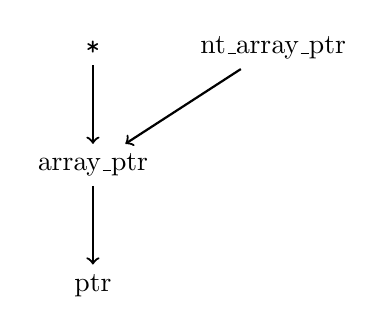
\begin{tikzpicture}[sibling distance=0.5in]
\node (ptr) {\ptr};
\node (arrayptr)   [above=of ptr]      {\arrayptr}    edge[->, thick] (ptr);
\node (unchecked)  [above=of arrayptr] {\texttt{*}} edge[->, thick] (arrayptr);
\node (ntarrayptr) [right=of unchecked] {\ntarrayptr}  edge[->, thick] (arrayptr);
\end{tikzpicture}
\end{center}
\caption{Ordering of pointer kinds by restrictiveness of operations and allowed conversions.}
\label{fig:pointer-kind-ordering}
\end{figure}

Second, the greatest lower bound of the pointer referent types for the arms is computed.
If the pointer referent types are the same type, that type is the greatest lower bound.
Otherwise, the greatest lower bound is the referent type that is at least as checked as the
other referent type and is otherwise compatible.  Given referent types \var{S} and \var{R},
we check assignment compatibility using each type as the destination.  We
choose the referent type for which assignment compatibility is valid.
If assignment compatibilty is not valid for either type, no greatest lower
bound exists and the implicit conversion is not allowed.

Void referent types are treated specially. They are considered to be lower than
corresponding non-void referent types because fewer operations are allowed on
void referent types. We require that the source referent
type in the assignment compatibility test not be the void type.
This matches the existing C rules for conditional expressions.  Those
rules state that if one arm has void pointer type, the other
arm must be implicitly cast to void pointer type.  Implicit casts from void pointers to other
pointer types are not allowed for conditional expression arms.

Here are some examples of greatest lower bounds:
\begin{itemize}
\item  For arms with the types \arrayptrint\ and \ptrint, it is \ptrint.
\item  For arms with the types \arrayptrvoid\ and \uncheckedptrinst{\keyword{int}},
it is \arrayptrvoid.
\item In contrast, for arms with the types \arrayptrinst{\keyword{float}} and \arrayptrinst{\keyword{int}}, none exists:
\keyword{float} is not assignment-compatible with \keyword{int}.
\end{itemize}

\subsection{Between checked pointers and integers}

The null pointer (\code{0}) can be converted implicitly to any checked pointer type.
A checked pointer can be converted implicitly to the \code{_Bool} type.

Some C compilers extend C by allowing implicit conversions between pointers
and integers or between pointers to incompatible types.  Implicit conversions
from integers to checked pointers are typically not useful in Checked C because
the checking of bounds declarations fails or the resulting pointer cannot
be used to access memory.   The rules for checking bounds declarations only
allow the target type to be \arrayptr\ type and the bounds of the expression to be
\boundsunknown.

\subsection{Examples}

The following code shows examples of implicit conversions.  In these examples,
the right-hand sides of assignments have the type ``unchecked pointer to
\var{T}'', while the left-hand sides have the type ``checked pointer to
\var{T}''.  Implicit conversions are done at those assignments.
\begin{lstlisting}
int x = 0;
ptr<int> px = &x;
array_ptr<int> pax : count(1) = &x;

int a[5] = { 0, 1, 2, 3, 4};
ptr<int> pa = a;
array_ptr<int> apa : count(5) = a;
array_ptr<int> middle : bounds(a, a + 5) =  a + 2;
\end{lstlisting}

An unchecked multidimensional array can be passed to a function expecting
a checked multi-dimensional array:
\begin{lstlisting}
int b[3][3] = { { 0, 1, 2}, { 3, 4, 5}, { 6, 7, 8}};
extern void f(int arg checked[3][3]);
f(b);
\end{lstlisting}

The mechanics behind this are somewhat complicated.  Parameters with type
``array of \var{T}'' are actually treated as having type ``pointer to \var{T}''.
Parameters with the type ``checked array of \var{T}'' are treated as ``checked
pointer to \var{T}''.  The actual type of the parameter of \code{f} is
\begin{lstlisting}
extern void f(array_ptr<int checked[3]> arg);
\end{lstlisting}
Local variables with type ``array of \var{T}'' are treated as having
type ``unchecked pointer to \var{T}'' when they are used.  The type of
\code{b} at \code{f(b)} is ``unchecked pointer to an array of 3 integers''.
At the call to  \code{f(b)}, there is an implicit conversion from an
``unchecked pointer to an unchecked array of 3 integers'' to a ``checked pointer
to a checked array of 3 integers'':
\begin{lstlisting}
int (*pb)[3] = b;
array_ptr<int checked[3]> param : count(3) = pb;
\end{lstlisting}
This implicit conversion is allowed because \lstinline|int checked[3]| is assignment
compatible with \lstinline|int[3]|.  Assignment compatibility allows other
interesting implicit conversions:
\begin{lstlisting}
array_ptr<int[3]> t1 : bounds(b, b + 3)  = b;
array_ptr<int> t2 : bounds(b, b + 3) = t1[1];
array_ptr<int> t3 : bounds(b, b + 3) = b[1];
\end{lstlisting}

\subsection{Non-examples}

Implicit conversions must still pass the bounds rules for the corresponding explicit
C cast operation.  Implicit conversions where the source bounds are not large
enough will be rejected during bounds declaration checking:
\begin{lstlisting}
int x = 0;
// fails to check: source not large enough
array_ptr<int> pax : count(5) : &x;
\end{lstlisting}

Implicit conversions of unchecked pointers with no bounds to checked pointers
will also be rejected:
\begin{lstlisting}
char *random(void);

void f(void) {
    // fails to check: random() has no bounds
    array_ptr<char> sp : count(1) = random(); 
}
\end{lstlisting}

\section{Bounds-safe interfaces to existing unchecked functions and variables}
\label{section:function-bounds-safe-interfaces}

The new pointer types capture specific properties of pointers. We would like to update
existing C code to use the new pointer types. This would be problematic for library and operating
system APIs that have backward  compatibility constraints, however.   Consider what would happen
if the signature for \code{memcpy} were changed to use \arrayptr. The function

\begin{lstlisting}
void *memcpy(void *dest, const void *src, size_t count);
\end{lstlisting}

would become

\begin{lstlisting}
void *memcpy(array_ptr<void> dest, array_ptr<const void> src,
                      size_t count);
\end{lstlisting}

This would break existing code that uses \code{memcpy}.  The code would no
longer type check.  The reverse problem also exists: suppose the signature for
\code{memcpy} is not updated.  Then every checked method that calls
\code{memcpy} would need to cast the arguments to unchecked pointer types.

Given that changing the types of existing APIs is problematic, we take an approach
that does not change types, yet enables new checked code to be written easily
and that maintains the checking of the new code.  We allow programmers to
declare {\em bounds-safe interfaces} that extend existing declarations with
additional bounds information.  

Bounds-safe interfaces can be 
specified for declarations of functions, global variables, and
data structures.  They can also be specified for function types.
The interfaces describe the expected behavior and the assumptions
of existing code about bounds. The types remain the same.
It is assumed but not verified that existing code
meets the specified interfaces.  A bounds-safe interface allows
checked code to use existing unchecked code safely with respect
to bounds, assuming that the interface and existing code are
correct.

Type checking is modified to insert implicit conversions between
checked types and unchecked types at bounds-safe interfaces.
The additional bounds information is used during checking
of bounds declarations to ensure that checked code is
using existing declarations properly.  It is also used to insert
bounds checks in checked code.  This allows new checked code to
use existing unchecked code, once a bounds-safe interface has
been added to the existing code.
\begin{enumerate}
\item
  In checked scopes, code is limited to using pointer types that are 
  checked pointer types or unchecked pointer types with bounds-safe interfaces.
  This makes the code in checked scopes straightforward to understand:
  the unchecked pointer types are regarded as checked pointer types, all memory
  accesses are bounds checked or in bounds, and bounds-safe interfaces are trusted
  and respected.
\item
  In unchecked scopes, checked and unchecked pointer types can be
  be intermixed within expressions.  When that happens, the bounds-safe
  interfaces are used during checking of bounds declarations to determine
  bounds of expressions and the required bounds for assignments and function calls. 
  Section~\ref{section:implicit-conversions} already
  explained when implicit conversions from unchecked pointer types to checked pointer
  types may be inserted.   Implicit conversions of expressions 
  from checked pointer types to unchecked pointer types are inserted when
  necessary at bounds-safe interfaces.
\end{enumerate}

The sections on bounds-safe interfaces are organized as
follows.  Section~\ref{section:bounds-safe-interface-specifying} describes
how to specify bounds-safe interfaces.
Section~\ref{section:bounds-safe-interface-examples}
has examples that show the use of bounds-safe interfaces.
Section~\ref{section:bounds-safe-interface-redeclaration} explains
how existing functions and variables can be redeclared with bounds-safe
interfaces.  Section~\ref{section:bounds-safe-interface-type-checking}
and ~\ref{section:checking-bounds-interfaces} cover technical details
about type checking and checking bounds declarations that are interesting
to language designers and compiler writers.  Programmers interested
in using the Checked C extension can skip those sections.

\subsection{Specifying bounds-safe interfaces}
\label{section:bounds-safe-interface-specifying}
Bounds-safe interfaces for declarations are specified by adding bounds
declarations or type annotations to declarations.  They can be added to
function declarations, function types, globally-scoped variables, and
declarations of members of structure and union types.
A declaration can have both a bounds declaration and a type annotation,
although it is less common to need both.

We describe adding bounds declarations first and then  describe adding type
annotations.  Functions that have parameters with unchecked pointer
or array types or that return values with unchecked pointer types can have bounds
or type annotations declared for the parameters and return values.  At calls to
these functions, implicit conversions from checked types to unchecked
pointer types are inserted for the corresponding argument expressions.
  
Here is a bounds-safe interface for \code{memcpy}:
\begin{lstlisting}
void *memcpy(void *dest : byte_count(len),
             const void *src : byte_count(len), 
             size_t len) 
             where return_value : bounds((char *) dest,
                                         (char *) dest + count);
\end{lstlisting}
The correctness of bounds information is enforced at compile-time when
\code{memcpy} is passed checked pointer arguments. It is not enforced when 
\code{memcpy} is passed unchecked pointer arguments.

Variables at external scope with unchecked pointer or array types
can have bounds or type annotations declared for them.
The declarations must follow the
rules in Section~\ref{section:external-scope-variables}.

For data structures, members with unchecked pointer type or array types
can have bounds or type annotations declared for them.   Implicit conversions from
\arrayptr\ type to unchecked pointer type are inserted at assignments to unchecked
pointer type members.

% Comment out because this isn't what the implementations does and it
% isn't clear these requireements are needed.
%
% Bounds-safe interfaces for functions and members must be
% declared on an ``all-or-nothing'' basis.
% For a function, if any parameter (or the return value) has an unchecked pointer
% or array type and has a bounds declaration or type annotation, all the
% the other parameters (or the return value) that have unchecked
% pointer or array types must also have bounds declarations or type
% annotations.  Similarly, for a structure or union type,
% if any member with unchecked pointer or array type
% has a bounds declaration or type annotation, all other members
% that have unchecked pointer types must also have bounds declarations
% or type annotations.

Here are the bounds for a structure that is a counted buffer of
characters.
\begin{lstlisting}
struct S {
  char *arr : count(len);
  int len;
}
\end{lstlisting}

It is important to understand that the \emph{semantics of unchecked
pointers and arrays do not change in unchecked scopes even when bounds
or type annotations are declared for the pointers and arrays}.
Unchecked pointer dereferences do not have bounds checks added to them.
Similarly, uses of unchecked arrays still convert to
unchecked pointer types. A function that has a bounds-safe
interface and whose body does not use checked pointer or array
types is compiled as though the bounds-safe interface has been
stripped from its source code. If the function body contains an expression
that mixes checked and unchecked pointer types, then the compiler uses
any declared bounds or interface type annotations on the unchecked pointer
types to infer and validate bounds. The example at the end of
Section~\ref{section:checking-bounds-interfaces} illustrates this point.

A type annotation describes an alternate checked type to use in checked code
in place of an unchecked type. It is used, for example, when a variable with
an unchecked pointer type should be treated as having
a \code{ptr} type.  Syntactically, a bounds declaration can have
a bounds expression, a type annotation, or both a bounds expression
and a type annotation.

A type annotation is specified using the following syntax:

\begin{tabbing}
\var{type-}\=\var{annotation:} \\
\>\code{itype (}\var{type name}\code{)}\\
\\
The keyword \code{itype} is short for bounds-safe  interface type.
\\
\\
The syntax for an inline bounds specifier is extended to
allow a type annotation or a bounds\\
expression and a type annotation:
\\
\\
\var{inline-bounds-specifier:}\\
\> \lstinline|:| \var{bounds-exp} \\
\>\code{:} \var{type-annotation} \\
\>\code{:} \var{bounds-exp} \var{type-annotation} \\
\>\code{:} \var{type-annotation} \var{bounds-exp}
\end{tabbing}

A type annotation can be used to declare that an unchecked
pointer to a structure should be treated as a \lstinline+ptr+ in
checked code. Here is a declaration for a function
\lstinline+count_char+ that takes
an unchecked pointer to the struct \code{S} defined earlier,
with a type annotation. \lstinline+count_char+ counts the number
of occurrences of \lstinline+arg+ in \lstinline+S+. Checked code must pass a
value that is a valid \lstinline+ptr+ to \lstinline+count_char+:
\begin{lstlisting}
int count_char(S *str : itype(ptr<S>), char arg);
\end{lstlisting}
A type annotation can be used to declare that an unchecked array member should
be treated as a checked array in checked code:
\begin{lstlisting}
struct S {
   int a[5] : itype(int checked[5]);
};
\end{lstlisting}

Here are functions from the C Standard Library with type annotations.
In the examples, type annotations for return types are placed 
after the parameter list, the same way that bounds expression for
return values are placed:
\begin{lstlisting}
double modf(double value, double *iptr : itype(ptr<double>));
int fclose(FILE *stream : itype(ptr<FILE>));
FILE *tmpfile(void) : itype(ptr<FILE>);
struct tm *gmtime(const time_t *timer : itype(ptr<const time_t>)) :
    itype(ptr<struct tm>);
\end{lstlisting}

A set of rules define interface type compatibility.
The \var{type name} in a type annotation must be compatible
with the original unchecked type when checkedness
of pointers and arrays is ignored. The \var{type name} cannot
lose checking.  It must be at least as checked as the
original type.  Finally, the \var{type name} must be
a checked type.   Checked types are defined inductively:
checked pointer and array types are checked types,
array and pointer types constructed from checked types
are checked types, and function types constructed from
at least one checked type are checked types.


\subsection{Examples}
\label{section:bounds-safe-interface-examples}

Here are some examples:
\begin{lstlisting}
void copy(array_ptr<int> dest : count(len),
              array_ptr<int> src : count(len), int len)
{
    // dest, src will be converted implicitly to void * pointers.
    // Even though this is an unchecked context, the function call
    // arguments will be checked to make sure that they meet the
    // bounds requirements of memcpy.  This is because the argument
    // expressions have checked pointer types.
    memcpy(dest, src, len * sizeof(int));
}

f(S s) 
{
     int len = s.len;
     array_ptr<char> sp : count(len) = s.arr;
     ...
     if (len > 0) {
        sp[0] = 'a';
     }
}
\end{lstlisting}

This example will fail at compile time:
\begin{lstlisting}
void bad_copy(int *dest, array_ptr<int> src : count(len), int len)
{
    // dest, src will be converted implicitly to void * pointers.
    // Because an argument had a checked pointer type, the function call
    // will be checked to make sure parameters meet the bounds
    // requirements.  This will fail because dest has no bounds.
    memcpy(dest, src, len * sizeof(int));
}
\end{lstlisting}

In contrast, this example will compile:
\begin{lstlisting}
void subtle_copy(int *dest, array_ptr<int> src : count(len), int len)
{
    // This function call will not be checked for bounds
    // requirements because no arguments have checked pointer
    // types.  This shows both that the programmer has control
    // over checking by using types and why checked contexts
    // should be used with checked pointers when possible (perhaps
    // the programmer did not want to do this).
    memcpy(dest, (void *) src, len * sizeof(int));
}
\end{lstlisting}

\subsection{Parameter array types}

In C, arrays are passed by reference as arguments.  During
type checking, the type of parameters with type ``array of \var{T}'' are
altered to \uncheckedptrT.  Before checking interface type
compatibility for a parameter, if the interface type is an array type,
it is altered to be a pointer type following the rules in
Section~\ref{section:array-to-pointer-conversion}.   The checking is
then done using the alted parameter type and altered interface type.
The original unaltered interface type is used when inferring bounds
and bounds requirements.

The following examples illustrate some possible bounds-safe interface
declarations for a parameter of type \lstinline{int **}:
\begin{lstlisting}
void f(int **p : itype(ptr<ptr<int>>));
void f(int **p : itype(ptr<array_ptr<int>>));
void f(int **p : itype(array_ptr<ptr<int>>));
void f(int **p : itype(array_ptr<array_ptr<int>>));
void f(int **p : itype(ptr<int *>));
void f(int **p : itype(array_ptr<int *>));
void f(int **p : itype(ptr<int> checked[10]));
void f(int **p : itype(ptr<int> checked[]));
void f(int **p : itype(array_ptr<int> checked[10]));
void f(int **p : itype(int *checked[20]));
\end{lstlisting}

\subsection{Function pointer type as parameter}
Function pointers that are parameters in a bounds-safe interface specification
can themselves have a bounds-safe interface type.  This allows both checked and
unchecked function pointers to be passed as actual arguments.
Here is an example:
\begin{lstlisting}
int apply_fun (
  char *buffer : itype(array_ptr<char>) count(length),
  size_t length,
  int ((*fun)(char *buf, size_t len)) :
      itype(ptr<int(array_ptr<char> buf : count(len), size_t len)>)
);
\end{lstlisting}

In the above example \lstinline+fun+ is a function pointer.  Note that an extra
pair of parentheses is required around the function pointer declaration before
the type annotation.  This is necessary to disambiguate parsing.  Without the
extra pair of parentheses, the compiler attempts to bind the itype (
\lstinline+ptr<int(array_ptr<char> buf : count(len), size_t len)>+) to the
return value of the function pointed to by \lstinline+fun+, which will result
in a compilation error.

\subsection{Bounds expression and type annotations}
A bounds-safe interface declaration can have both a bounds expression and a type
annotation.  This allows programmers to declare bounds-safe interfaces for declarations involving
nested pointer types.

Consider a bounds-safe interface for \lstinline{char **p}.
The checked type for the variable can be declared using a type annotation
and the bounds for the variable can be declared using a bounds expression.
\begin{lstlisting}
char **p : itype(ptr<ptr<char>>);
char **p : itype(ptr<nt_array_ptr<char>>);
char **p : count(len) itype(array_ptr<ptr<char>>)
char **p : count(len) itype(array_ptr<nt_array_ptr<char>>);
char **p : itype(nt_array_ptr<ptr<char>>);
char **p : count(4) itype(nt_array_ptr<nt_array_ptr<char>>);
\end{lstlisting}

If only a bounds expression is placed on a declaration of a variable with type \uncheckedptrinst{T},
it implies that the type annotation is \arrayptrinst{T}.   If it is placed on a variable with an
array type \lstinline{T[D]}, it implies that the type annotation is \lstinline{T checked[D]}.   If
an interface type and a bounds expression are both specified, the interface type must
be an \arrayptr\ type or checked array type.

\subsection{Redeclaring existing functions and variables with bounds-safe interfaces}
\label{section:bounds-safe-interface-redeclaration}

C allows variables or functions to be declared with types that are missing information.
There can be other declarations of the variables or functions with types that are more complete
and fill in the missing information.  The types that are missing information are said to be
``compatible'' with the more complete versions of the types.  Multiple declarations of
a variable or function are required to have compatible types, not identical types.

This notion of compability extends to bounds-safe interfaces naturally.  We extend the
definition of compatibility of function types in Section~\ref{section:function-types} as follows:
\begin{itemize}
\item Given corresponding parameters with compatible unchecked pointer types,
one parameter may have a bounds declaration and one parameter may omit the bounds declaration.
\item Given return values with compatible unchecked pointer types, one
return value may have a bounds declaration and one return value may omit the bounds declaration.
\end{itemize}

The following are examples of declarations of functions with compatible types:
\begin{lstlisting}
int f(int *);
int f(int * : count(5));

int g(int *a, int len, int *b);               // decl 1
int g(int *a : count(len), int len, int *b);  // decl 2
int g(int *a, int len, int *b : count(len));  // decl 3
int g(int *a : count(len), int len, int *b : count(len));  // decl 4
\end{lstlisting}
The declarations of \code{g} are particularly interesting. They are all
compatible declarations.  The only version
that could be used in a checked scope is declaration 4.   For declarations 2 and 3,
where bounds information is missing for a parameter, the argument passed to \code{g}
for that parameter cannot have an \arrayptr\ type.  The typing rules prevent arguments
with checked type from being used with parameters of \code{g} that are missing
bounds information.

\subsection{Type checking}
\label{section:bounds-safe-interface-type-checking}

Bounds-safe interfaces allow unchecked pointer types to be used
where checked pointer types with assignment compatible referent types are
expected and {\it vice versa}.
To handle this, implicit pointer conversions are inserted during type checking.
Section~\ref{section:implicit-conversions} covered implicit conversions from unchecked pointer types to checked pointer types.

Implicit conversions from checked pointer types to unchecked pointer types
with assignment-compatible referent types are allowed at the uses of functions,
variables, or members with bounds-safe interfaces, and at return statements.  
In this case, assignment compatibility is applied in a reverse fashion (assignment compatibility
is defined in Section~\ref{section:implicit-conversions}).
The source referent type must be
assignment compatible with the destination referent type.  The conversions are
done for rvalue expressions by inserting C cast operators to the desired unchecked types.
They are done at:
\begin{itemize}
\item Function call arguments: If the function being called has a
      bounds-safe interface for parameters with unchecked pointer types, a parameter
      has an unchecked pointer type, the corresponding argument expression
      has a checked pointer type, and the argument referent type is assignment
      compatible with the parameter referent type, then the argument expression
      will be converted implicitly to the unchecked pointer type.
\item Assignments to variables with external scope: if the variable being
     assigned to has an unchecked pointer type and a bounds-safe interface, the
     right-hand side expression has a checked pointer type, and the right-hand
     side expression referent type is assignment compatible with the referent
     type of the variable, then the right-hand side expression will be converted
     implicitly to the unchecked pointer type.
\item
    Member assignments: a similar conversion is done for member assignments.
\item Assignments to pointer dereferences: if the pointer dereference expression
  being assigned to has an unchecked pointer type and a bounds-safe interface, the
  right-hand side expression has a checked pointer type, and the right-hand side
  expression referent type is assignment compatible with the referent type of the
  pointer dereference expression, then the right-hand side expression will be
  converted implicitly to the unchecked pointer type.
\item Assignments to array subscripts: if the array subscript expression being
  assigned to has an unchecked pointer type and a bounds-safe interface, the
  right-hand side expression has a checked pointer type, and the right-hand
  side expression referent type is assignment compatible with the referent
  type of the array subscript expression, then the right-hand side expression
  wil be converted implicitly to the unchecked pointer type.
\item Assignments to null-terminated arrays: if the left-hand side expression
  being assigned to has a checked null-terminated array type, the right-hand side
  expression has an unchecked null-terminated array type and a bounds-safe interface,
  and the referent type of the right-hand side expression is assignment compatible
  with the referent type of the left-hand side, then the right-hand side expression
  will be converted implicitly to the checked null-terminated array type.
\item Return statements: if a function has an unchecked pointer return type and a
  return bounds-safe interface, and a return statement in the body of the function
  has an expression with a checked pointer type, and the return statement expression is
  assignment compatible with the return type of the function, then the return expression
  will be converted implicitly to the unchecked pointer type.
\end{itemize}

Implicit conversions at bounds-safe interfaces are allowed from checked pointer types to
\uncheckedptrvoid.  This rule is likely to change in the future.  There is not a  design for
checking type-safety of casts yet and the design will amost certainly affect 
\uncheckedptrvoid\ casts.

Only one implicit pointer conversion is allowed for an expression at a bounds-safe
interface.  For example, an expression will not be
coerced implicitly from \ptrinst{\var{S}} to \uncheckedptrvoid\ to
\uncheckedptrinst{\var{T}}, where \var{S} and \var{T} are different types.

\subsection{Checking bounds declarations}
\label{section:checking-bounds-interfaces}

The checking rules in Chapter~\ref{chapter:checking-bounds} require
only small changes to check code with bounds-safe interfaces.  The
checking is done after any implicit pointer conversions have been
inserted.
\begin{itemize}
\item Contexts are extended to include unchecked pointer variables with
      bounds-safe interfaces.
\item Inference of bounds of expressions (Section~\ref{section:inferring-expression-bounds}) incorporates information from bounds-safe interfaces:
\begin{itemize}
\item Uses of variables (Section~\ref{section:checking-variables}): 
      if a variable with an unchecked pointer type is used and the context has
      a bounds for the variable, the bounds in the context are used as the bounds
      for the variable.
\item Function calls (Section~\ref{section:inferring-bounds-for-function-calls}): 
      the rules in this section are also applied when a function returns an unchecked
      pointer value and the return value has a bounds-safe interface.
\end{itemize}
\item The checking that an expression statement, declaration, or bundled
      block implies the declared bounds of variables includes:
\begin{itemize}
\item In checked contexts, all variables with bounds-safe interfaces.
\item In unchecked contexts, all variables with bounds-safe interfaces
      that are modified by an assignment within the statement, declaration,
      or bundled block, where the right-hand side expression
      is converted implicitly from a checked pointer type to an unchecked pointer type.
\end{itemize}
For the included variables, bounds are tracked through the statement or
bundled block.
\item The checking of function call arguments
      in function calls (Section~\ref{section:checking-function-call-arguments})
      includes parameters with bounds-safe interfaces:
\begin{itemize}
\item In checked contexts.
\item In unchecked contexts, when one or more argument expressions have been
      converted implicitly to unchecked pointer types.
\end{itemize}
The parameters are included by adding their bounds-safe interfaces to the
declared bounds in the constructed \keyword{where} clauses.
\item The checking of return statements (Section~\ref{section:checking-return-statements})
includes return statements where there is a return bounds-safe interface for the enclosing function:
\begin{itemize}
\item In checked contexts.
\item In unchecked contexts, when the return statement expression has been converted
      implicitly to an unchecked pointer type.
\end{itemize}
The return bounds-safe interface is used in place of the function return bounds.
\end{itemize}

The checking for assignments and function calls has some interesting 
implications in unchecked contexts.  It is possible to have a statement, 
a declaration, or a bundled block that mixes different kinds of pointers
in assignments to the same  variable.  
Some right-hand sides could have checked pointer types and others
could have unchecked pointer types.  This is a programming practice that is discouraged.
Nevertheless, the bounds declarations will be checked no matter which
kind of assignment is the last one.  This implies that if the last 
assignment has an unsafe pointer-typed right-hand side, it will still need
to have valid bounds. If a subexpression of a comma expression mixes checked and
unchecked pointer types, then that subexpression will be checked.
It is also possible to mix argument expressions with
checked and unchecked  pointer types in one function call.  The checking of bounds
for function arguments is done for all arguments, so this also implies that the unchecked
pointer-typed expressions will need to have valid bounds.

Here is some example code that illustrates the behavior of the compiler:
\begin{lstlisting}
extern int *lib_func_1(_Array_ptr<int> p);
extern int *lib_func_2(_Array_ptr<int> p) : itype(_Array_ptr<int>);
extern _Array_ptr<int> lib_func_3(_Array_ptr<int> p);

int *foo(int *p : count(2), int *r : count(n), unsigned n) : count(4)
_Unchecked {
  _Array_ptr<int> chk : count(1) = 0;

  n++;                   // The declared bounds of r are not validated.
  r = p;                 // The declared bounds of r are not validated.
  r = chk;               // The declared bounds of r are validated.
  chk = 0, n = 0;        // The declared bounds of r are not validated.
  p = chk, p++;          // The declared bounds of p are validated.
  p = chk, n++;          // The declared bounds of p are validated
                         // but not of r.
  r = chk, n++;          // The declared bounds of r are validated.
  r = lib_func_1(chk);   // The declared bounds of r are not validated.
  r = lib_func_2(chk);   // The declared bounds of r are not validated.
  r = lib_func_3(chk);   // The declared bounds of r are validated.

  if (n < 5)
    return p;      // The return bounds are not checked.

  else if (n < 10)
    return chk, p; // The return bounds are not checked as the type of
                   // the return value expression chk, p is int *.
  else
    return p, chk; // The return value bounds are checked as the type
                   // of the return value expression p, chk is
		   // _Array_ptr<int> (which is implicitly cast to int *).
}
\end{lstlisting}


\section{Bounds-safe interfaces for generic functions and struct types}
\label{sec:generic-bounds-safe-interfaces}
This section describe how to provide bounds-safe interfaces for existing functions
that are actually generic. It extends the examples in Section~\ref{sec:generic-functions}.

Here is the existing bounds-safe interface for \lstinline+bsearch+. 
The bounds declaration on \uncheckedptrvoid{} results in a parameter being
treated as having type \arrayptrvoid{} in checked code:
\begin{lstlisting} 
// Current Checked C version declaration
void *bsearch(const void *key : byte_count(size),
              const void *base : byte_count(nmemb * size),
              size_t nmemb, size_t size,
              int ((*compar)(const void *, const void *)) :
                itype(ptr<int(ptr<const void>, ptr<const void>)>)) :
                byte_count(size);
\end{lstlisting}
To declare that a bounds-safe interface for a function that is generic, we precede
the function declaration with an \lstinline+itype_for_any(...)+ clause.
Here is a version of \lstinline+bsearch+ modified this way:
\begin{lstlisting}
// Generic Checked C version
itype_for_any(T)
void *bsearch(const void *key : itype(ptr<const T>),
              const void *base : itype(array_ptr<const T>) byte_count(nmemb * size),
              size_t nmemb, size_t size,
              int ((*compar)(const void *, const void *)) :
              itype(ptr<int (ptr<const T>, ptr<const T>)>)) : itype(ptr<T>);
\end{lstlisting}
The \lstinline+itype_for_any(T))+ indicates that \lstinline+bsearch+ has a generic
bounds-safe interface.   The type variable \lstinline+T+ is available in the
bounds-safe interface declarations for parameters and return values.  The parameter 
\lstinline+base+ has both an itype and a bounds declaration.

Here are bounds safe-interfaces for other C standard library
functions:
\begin{lstlisting}
itype_for_any(T) void *malloc(size_t size) :
                    itype(array_ptr<T>) byte_count(size);

itype_for_any(T) void *calloc(size_t nmemb, size_t size : sizeof(T)) :
                    itype(array_ptr<T>) byte_count(nmemb * size);

itype_for_any(T) void free(void *pointer : itype(array_ptr<T>) count(1));

itype_for_any(T) void *memcpy(void * restrict dest :
                                 itype(array_ptr<T>) byte_count(n),
                               const void *T src :
                                 itype(array_ptr<T>) byte_count(n),
                               size_t n where n % sizeof(T) == 0) :
                                 itype(array_ptr<T>) byte_count(n);
\end{lstlisting}

The bounds-safe interfaces act as follows.  When a function 
is applied to type arguments, the type arguments are substituted
for the type variables to construct the concrete function type.
For parameters and returns that have bounds-safe interfaces, the
bounds-safe interfaces are used for their types.

Type parameters are mandatory in calls
to generic bounds-safe interface functions from checked scopes.
Type parameters are optional in unchecked contexts. When a 
function with a generic bounds-safe interface is called
without type variables from unchecked code, we apply void type
for the type variables.

Consider as an example \lstinline+bsearch<int>+.  First a concrete
function type is constructed:
\begin{lstlisting}
void *(const void *key : itype(ptr<const int>),
       const void *base : itype(array_ptr<const int>) byte_count(nmemb * size)),
       size_t nmemb, size_t size,
       int ((*compar)(const void *, const void *)) :
           itype(ptr<int (ptr<const int>, ptr<const int>)>)) : itype(ptr<int>);
\end{lstlisting}
Then, bounds-safe interfaces for parameters and returns are used as
their types:
\begin{lstlisting}
ptr<int> (ptr<const int> key,
               array_ptr<int> base : byte_count(nmemb * size),
              size_t nmemb, size_t size,
              ptr<int (ptr<const int>, ptr<const int>)> compar);
\end{lstlisting}
Now, suppose \lstinline+bsearch+ is called without applying it to type variables.
In that case, any itypes that use a type variable are discarded:
\begin{lstlisting}-
void *(const void *key,
         const void *base : byte_count(nmemb * size),
         size_t nmemb, size_t size,
         int ((*compar)(const void *, const void *)));
\end{lstlisting}

\section{Conversions between pointers and integers}
\label{section:pointer-integer-conversions}

C allows pointers to be converted to suitably large enough integer
types and then converted back to pointers.  Integer operations can
done on the converted values before they are converted back.
This is one of the features of C that leads people to 
say that C cannot possibly be made type-safe.  In this section,
we explain how casts between pointers and integers within 
expressions can be controlled and reasoned about.

\subsection{Tagged pointers}
We start with a motivating example, tagged pointers.
C programs sometimes store information in unused bits of pointers
to save on space in data structures.  Other times this is done
to acheive atomicity when reading or writing data.  A
program might store a tag in the least significant bits or most
significant bits of some pointers, knowing that those bits are always
zero otherwise.

The bounds of such a pointer are easy to describe: they are the bounds
of the original pointer. If a pointer variable or member is used in its
own bounds, the tag must be removed first. This is
done by masking out the bits that are always 0.

For example, suppose there is the following structure:

\begin{lstlisting}
struct S {
  array_ptr<int> p : bounds(p, p + 4);
  int tag : 2;
}
\end{lstlisting}

A programmer might know that on a machine with 32 bit pointers, the
least 2 significant bits of p are always 0, so the tag could be stored
within p. The bounds would be changed to:

\begin{lstlisting}
struct S {
  array_ptr<int> p : bounds((array_ptr<int>) ((size_t) p & ~3), 
                            (array_ptr<int>) ((size_t) p & ~3) + 4) rel_align(char);
}
\end{lstlisting}

There is one important caveat (for now): tags cannot be stored in null pointers. A
null pointer may have bounds that are not valid. This is fine because
the null pointer may not be used to access memory. However, tagging a
null pointer could result in a non-null pointer with bounds that are
invalid. This pointer could be used to access memory incorrectly.

\subsection{Extending bounds checking rules to integral
expressions}

The inference of bounds for expressions disregards non-narrowing cast operators:
the  information flows through the operation, with adjustments if the bounds
include \exprcurrentvalue.  This makes it straightforward to extend the
rules for inferring bounds to integral expressions:

\begin{itemize}
\item
  Given \var{e1} \var{op} \var{e2}, where \var{op} is an additive, multiplicative, or bitwise
  binary operator on integral types, the bounds of \var{e1} and \var{e2} can be
  computed:

  \begin{itemize}
  \item
    If \boundsdecl{\var{e1}}{\var{b}}, where \var{b} is not \boundsunknown, and 
    \boundsdecl{\var{e2}}{\boundsunknown}, and it can be proved that \var{e1} \code{!= 0}, then
    \boundsinfer{\var{e1} \var{op} \var{e2}}{\var{b}}.
  \item
    If the special variable \exprcurrentvalue\ occurs in \var{b}:
    \begin{itemize}
    \item
      If \var{op} has an inverse operation \var{inverse-op}, then 
      \exprcurrentvalue\ \var{inverse-op} \var{e2} is substituted for \exprcurrentvalue.
    \item
      Otherwise the bounds of the expression are altered to be \boundsunknown.
    \end{itemize}
  \item
    Similar rules apply for the reverse situation where \boundsdecl{\var{e1}}{\boundsunknown}
    and \boundsdecl{\var{e2}}{\var{b}}, where \var{b} is not \boundsunknown.
  \end{itemize}
\item
  Given \var{e1} \var{op} \var{e2} where \var{op} is a shift operator, \var{e1} is the integral value
  being shifted, and \var{e2} is the shift amount,

  \begin{itemize}
  \item
    If \boundsdecl{\var{e1}}{\var{b}}, where \var{b} is not \boundsunknown, and \var{e2} has
    \boundsunknown, and it can be proved that \var{e1} \code{!= 0}, then \boundsinfer{\var{e1} \var{op} \var{e2}}{\var{b}}.
  \item
    If the special variable \exprcurrentvalue\ occurs in \var{b},
    bounds of the expression are altered to be \boundsunknown. Shift
    expressions are not invertible because they lose information.
  \end{itemize}
\end{itemize}

\subsection{An example}

The following example shows functions for tagged pointers
(where the tag is stored in the least siginficant bit) that
create a tagged pointer and that set the tag to 1.

\begin{lstlisting}
#define untagged_bounds(x) \
   bounds((array_ptr<int>) ((size_t) x & ~0x1), \
          (array_ptr<int>) ((size_t) x & ~0x1) + 1) rel_align(char)

array_ptr<int> create(void) 
where untagged_bounds(return_value)
{
   array_ptr<int> x : bounds(x, x + 1) = malloc(sizeof(int));
   dynamic_check(x == (array_ptr<int>) ((size_t) x & ~0x1));
   // follows from substituting the right-hand side in the current bounds
   where x : untagged_bounds(x); 
   return x;
}

// set tag to 1
array_ptr<int> set(array_ptr<int> x : untagged_bounds(x)) 
where untagged_bounds(return_value)
{
  if (x != NULL) {
     // ((size_t) x | 1) has the same bounds as x                   
     array_ptr<int> tmp : untagged_bounds(x) = (array_ptr<int>) ((size_t) x | 1);
     dynamic_check((size_t) tmp & ~0x1 == (size_t) x & ~0x1);
     // follows from substituting the right-hand side of the
     //dynamic check expression in the current bounds for tmp
     where tmp : untagged_bounds(tmp);
     return tmp;
  }
  return x;
}
\end{lstlisting}

\subsection{Allowing bounds to be declared for integer-typed variables}

We have described how bounds can be inferred for an expression with
casts between pointers and integers.  A programmer may want to
introduce variables for the results of subexpressions of an
expression or may not be able to do all of a computation within an expression.
To allow more general handling of casts between pointers and
integers, we allow bounds to be declared for integer-typed variables.
This may seem confusing, but it is a natural extension to tracking the
bounds for pointer values that have been cast to integers.   The \lstinline+set+
function can be written to use temporary variables instead:
\begin{lstlisting}
array_ptr<int> set(array_ptr<int> x : untagged_bounds(x))
where untagged_bounds(return_value)
{
  if (x != NULL) {
     size_t raw : untagged_bounds(raw) = (size_t) x;
     size_t tagged : untagged_bounds(raw) = raw | 1;
     dynamic_check(raw & ~0x1 == tagged & ~0x1);
     // bounds follow from substituting the right-hand side of the
     // dynamic check expression in the bounds for tagged.
     array_ptr<int> result : untagged_bounds(result) = (array_ptr<int>) tagged
     return result;
  }
  return x;
}
\end{lstlisting}

\section{Restricted interoperation with functions without prototypes}
C allows declarations of functions that do not specify the type of their parameters
(no-prototype function declarations).  This provides backward compatibility between
ANSI C from 1989 and earlier versions of C that did not check the types of
arguments at calls.  Using functions declared this way is
dangerous.  Arguments are passed based on their types and an incorrect call can be made
where the types of arguments do not match the types of the parameters of the function
definition.  This could lead to bypassing of checking.  Checked pointers could be 
converted silently to unchecked pointers or vice versa.  Even worse, parameters could contain
corrupted values or the stack could be corrupted.

We recommend strongly that programmers do not declare functions without prototypes.  This
feature is a backward compatibility feature and is used rarely now.
The GCC and clang C compilers have warning flags that will detect the declaration of functions without 
prototypes.

For checked scopes, the declaration or use of functions with no prototypes is an error
and is not allowed.   In unchecked scopes, forbidding the use of function
declarations without prototypes would violate the design goal of providing backward compatibility.
Instead, we restrict the usage of no-prototype functions to reduce the possibility of
bounds checking being bypassed accidentally in unchecked blocks.

Informally, we want to prevent values with checked types from being passed as arguments or
returned from calls to no-prototype functions.  This requires some care to define because of
structures, unions, and function pointers. We define the set of types $E$ that are an error to use
with functions without prototypes by induction.  It includes:
\begin{enumerate}
\item Checked pointer and array types.
\item Complete structure and union types with members that have types in $E$.
\item Pointers to function types that have argument or return types that are in $E$.
\item Complete structure and union types with members with bounds declarations (these
      are described in Chapter~\ref{chapter:structure-bounds}).
\item Pointers to function types with bounds declarations.
\end{enumerate}
Clauses 4 and 5 handle the case of integer-typed values that have bounds declarations
(note that bounds-safe interfaces on unchecked pointer types are not bounds declarations).

We define the following rules for unchecked scopes:
\begin{enumerate}
\item It is an error to call a function that is
declared to have no prototype and pass or return a value whose type is in $E$.
\item A function declaration with no prototype is incompatible with a function declaration
with a prototype that has parameter types or a return type in $E$ or that has bounds
declarations.
\end{enumerate}

\subsection{Examples of errors caught by rules}
The rules catch common errors.  They catch passing a checked pointer
to a function with no prototype:
\begin{lstlisting}
int f();

int g(ptr<int> a) {
  f(a);  // error - passing a checked type to a function without a prototype
}
\end{lstlisting}
They also catch redeclaring a function with no prototype to have a checked parameter:
\begin{lstlisting}
int f();

struct S {
  array_ptr<int> ap : count(len);
  int len;
}

// Error - incompatible definition of f with a prototype.
int f(S y) {
 ...
 }
\end{lstlisting}
By rule 2, the definition of \lstinline+f+ is incompatible with the initial
declaration of \lstinline+f+, so this is an error.  It is an error even
if \lstinline+S+ is an incomplete type at the time of
a prototype declaration for \lstinline+f+:
\begin{lstlisting} 
int f();

struct S;

int f(S y);  // Declarations involving incomplete types are allowed.

// Now define struct S.
struct S {
  array_ptr<int> ap : count(len);
  int len;
}

// Error - incompatible definition of f with the initial declaration of f.
int f(S y) {
 ...
}
\end{lstlisting}

\subsection{Example of errors not caught by the rules}
The rules are not foolproof, though. Checking can be bypassed by code that
declares a function with no prototype in one
compilation unit and defines it in another compilation unit:
\begin{lstlisting}
Compilation unit 1:

int g(ptr<int> x) {
 ...
 }

Compilation unit 2:

extern int g();
void h(void) {
  g(5);  // Error
}
\end{lstlisting}
The definition of \lstinline+g+ in compilation unit 1 is incompatible with
the declaration in compilation unit 2, but there is no way for a compiler
to detect this.

The checking could be deferred to linking. The compiler could decorate the linker names of
functions whose argument types or return types are in $E$ differently from the names 
of functions whose argument types and return types are not in $E$.

\subsection{Unchecked pointers to checked types}
There is a limited way in which no-prototype functions can interoperate with checked types.
The definition of $E$ allows unchecked
pointers to checked pointers and arrays
to be passed to or returned from no-prototype functions.  It also allows unchecked pointers to
structures or unions that have checked members to be passed to or returned from
no-prototype functions.  Finally, it allows unchecked pointers with bounds-safe interfaces to be
passed to functions with no prototypes.  This is necessary so that bounds-safe interfaces
can be added to existing code without breaking the code.   

Here are some examples:
\begin{lstlisting}
int g();

int g(ptr<int> *x);

int f();

struct S {
  array_ptr<ptr> ap : count(len);
  int len;
}

int f(S *arg);
\end{lstlisting}

There are three reasons to allow unchecked pointers that point to checked data to
be passed to functions without prototypes.  First, the unchecked pointer types 
indicate a lack of checking, so it is already clear from the types of the variables being
used that there is some lack of checking.  Second, we believe that this
will support incremental conversion of code to use the Checked C extension.  Finally,
it would be difficult to enforce that an unchecked pointer does not point
to a checked type. An unchecked pointer could point to an incomplete
structure or union type. A compilation unit might never define the type. The type
could even be unresolved during linking of a library if none of the library compilation units
define the type.

% !Tex root = checkedc.tex

\chapter{Bounds declarations for structure types}
\label{chapter:structure-bounds}

This chapter extends reasoning about bounds to objects with structure
types by introducing bounds declarations for structure members.
Structure types may have members with \arrayptr\ types. Those
members must have \emph{member bounds declarations} associated with them in order for
the values stored there to be used to access memory.

The declarations of
structure members may include \keyword{where} clauses that declare member
bounds. The member bounds declarations may also be placed inline.
A structure declaration may also include \keyword{where} clauses at the same
level as member declarations.  Here are examples:

\begin{lstlisting}
struct S {
    array_ptr<int> data where data : count(num);
    int num;
};
\end{lstlisting}
or
\begin{lstlisting}
struct S {
    array_ptr<int> data : count(num);
    int num;
};
\end{lstlisting}
or
\begin{lstlisting}
struct S {
    array_ptr<int> data;
    int num;
    where data : count(num);
};
\end{lstlisting}

Member bounds declarations are program invariants that are assumed to be true
by default for objects of that type.

Making member bounds declarations be invariants provides a way to deal with issues
caused by aliasing. There can be pointers to data structures or members
of data structures. There may be multiple pointers to a single
structure object in memory. When there are multiple pointers,
the pointers are called aliases because they all name the same
memory location.  Aliasing makes it hard to reason about programs.

Consider the example:
\begin{lstlisting}
f(S *q, S *r, bool b)
{
   if (b) {
      q->arr = malloc(sizeof(int)*5);
      q->len = 5;
   }
   else {
      r->arr = malloc(sizeof(int)*5);
      r->len = 5;
   }
}
\end{lstlisting}

Even when b is true, the value \code{r->arr} may still be
changed by a call to f. This can happen when \code{q} and \code{r}
are the same value and are aliases for the same memory location.
Changing one named value (\code{q->arr}) can have the
effect of changing some other value with a distinct name
(\code{r->arr}). In general, it is difficult to know
whether an assignment through one pointer variable is affecting the
members of other pointer variables.

Member bounds declarations being program invariants for structure members allows
localized reasoning about the members. A programmer can assume that the
bounds declarations are true for members of objects of that type.

In the rest of this chapter, to simplify the description, assumptions
about address-taken variables similar to those in
Section~\ref{section:bounds-declarations} are made.
It is assumed that none of the variables or members of variables on the
left-hand side of bounds-declarations have their addresses taken. It is
assumed also that the values of variables or members of variables whose
addresses are taken are not used in bounds expressions.

\section{Declaring bounds for structure members}

Member bounds declarations have the form:
\begin{tabbing}
\var{member}\=\var{-bounds-decl:}\\
\> \var{member-path} \code{:} \var{member-bounds-exp} \\
\\
\var{member-path:}\\
\> \var{identifier} \\
\> \var{member-path} \code{.} \var{identifier}
\end{tabbing}

A member path is a sequence of one or more member names, separated by
the `\code{.}' operator. The sequence of members must be a valid sequence of
member accesses for the structure type. The common case of using a
member of the structure type is simply a member path of length 1.

Member bounds expressions are similar to the bounds expressions
described in Section~\ref{section:bounds-declarations}, 
except that members of the structure type are
used in place of variables in the non-modifying expressions. In
addition, pointer indirection and indirect member references are
excluded.

A structure member whose type is \arrayptr\ or a
checked array type may have at most one bounds declared for it. The
typing rules for member bounds declarations are similar to those for
variable bounds declarations. For bounds declarations of the form
\boundsdecl{\var{member-path}}{\boundscount{\var{e1}}}, the
\var{member-path} cannot have the type \arrayptrvoid\ and
the expression \var{e1} must have an integral type. For bounds declarations
of the form \boundsdecl{\var{member-path}}{\bounds{\var{e1}}{\var{e2}}},
the types of \var{e1} and \var{e2} must be pointers to the same type.
Typically \var{member-path} is also  a pointer to that type or an
array of that type.  However, \var{member-path} can be a pointer to
or an array of a different type.

A structure consists of a list of member declarations, each of which
consists of a type specifier followed by one or more structure member
declarators. Structure member declarators are changed to allow 
optional in-line specification of member bounds and \keyword{where}
clauses.

\begin{tabbing}
\var{struct}\=\var{-member-declarator:}\\
\> \var{declarator where-clause\textsubscript{opt}} \\
\> \var{declarator\textsubscript{opt}} \code{:}
   \var{constant-expression} \\
\> \var{declarator} \code{:} \var{member-bounds-exp}
\var{where-clause\textsubscript{opt}} \\
\\
The list of member declarations is extended to include \keyword{where}
clauses:\\
\\
\var{struct-member-declaration:}\\
\> \ldots{} \\
\> \var{where-clause}\textsubscript{opt}  \\
\\
The remaining syntax for specifying a structure remains unchanged: \\
\\
\var{struct-or-union-specifier:}\\
\> \var{struct-or-union identifier\textsubscript{opt}} \lstinline|{|
\var{struct-member-declaration-list} \lstinline|}| \\
\\
\var{struct-member-declaration-list:} \\
\> \var{struct-member-declaration} \\
\> \var{struct-member-declaration-list struct-member-declaration} \\
\\
\var{struct-member-declaration:} \\
\> \var{specifier-qualifier-list struct-member-declarator-list} \code{;} \\
\\
\var{struct-member-declarator-list:} \\
\> \var{struct-member-declarator} \\
\> \var{struct-declarator-list} \code{,} \var{struct-member-declarator} 
\end{tabbing}

A member bounds expression can use members and child members of the
structure being declared. Any member paths occurring in the member
bounds expressions must start with members of the structure type being
declared. Here is an example of the use of child members:

\begin{lstlisting}
struct A {
   array_ptr<int> data;
};

struct N {
    int num;
};

struct S {
   A a
   where count(a.data) == n.num;
   N n;
};
\end{lstlisting}

Allowing member bounds to use nested members of members complicates
explaining concepts. Sometimes concepts will be explained using member
bounds that use only immediate members and then generalized to handle
nested members.

\section{Bounds-safe interfaces}
\label{section:structure-bounds-safe-interfaces}

Just as existing functions can have bounds-safe interfaces declared for
them, existing structure types can have bounds-safe interfaces declared
for them. This allows checked code to use those data structures and for
the uses to be checked. Existing unchecked code is unchanged.
To create a bound-safe interface for a structure type, a programmer
declares member bounds or interface types for structure members with
unchecked pointer types.

Here is a member bounds declaration for a structure that is a counted buffer
of characters:

\begin{lstlisting}
struct CountedBuffer {
     char *arr : count(len);
     int len;
}
\end{lstlisting}

Here are bounds-safe interface types for members of a structure for binary
tree nodes. The structure contains pointers to two other nodes.  In
checked code, pointer arithmetic on those pointers is not allowed.

\begin{lstlisting}
struct BinaryNode {
    int data;
    BinaryNode *left : itype(ptr<BinaryNode>);
    BinaryNode *right : itype(ptr<BinaryNode>);
}
\end{lstlisting}

If bounds information is declared for one member of a structure with an
unchecked pointer type, it must be declared for all other members of the
structure with unchecked pointer types.

It is important to understand that the \emph{semantics of unchecked
pointers in unchecked contexts does not change even when bounds are declared 
for the pointers}. The declared bounds are used only by checked code that uses the
data structure, when storing checked pointers into the data structure, and when converting
unchecked pointers read from the data structure to checked pointers.  Code in unchecked
contexts that uses only unchecked pointer types is compiled as though the bounds-safe
interface has been stripped from the source code.

\section{Compatibility of structure types with bounds declarations}

The C Standard defines compatibility of two structure types declared in
separate translation units \cite[Section 6.2.7]{ISO2011}.  This definition
is extended to include member bounds declarations and member bounds-safe
interfaces.  If the structure types are completed in both translation
units, for each pair of corresponding members,
\begin{itemize}
\item If the members have unchecked pointer type,
\begin{itemize}
\item If the members both have bounds-safe interfaces, the bounds-safe
interfaces must either both be bounds expressions or both be interface
types. If both have bounds expressions, the bounds expressions must be
syntactically identical after being placed into a canonical form.
If both have interface types, the interface types must be compatible.
\item Otherwise,  one member must have a bounds-safe interface and the
other member must omit a bounds-safe interface, or both members must omit
bounds-safe interfaces.
\end{itemize}
\item Otherwise, both members must have member bounds declarations or both
members must not have member bounds declarations.  If both members have
member bounds declarations, the bounds expressions must be syntactically
identical after being placed into canonical form.
\end{itemize}

% !Tex root = checkedc.tex

\chapter{Pointers  to data with \plainarrayptr s}
\label{chapter:pointers-to-data-with-arrayptrs}

This chapter covers using pointers to data with \arrayptr s.  It also covers rules
around pointers and bounds expressions.  This includes dereferencing pointers
in bounds expressions and rules around address-taken pointer variables and
bounds expressions..
Three important scenarios for using pointers to \arrayptr s to support are:
\begin{itemize}
\item Data structures: All linked data structures in 
C are built with pointers, typically using pointers to structures.   This means
there need to be ways to create pointers to structures that contain \arrayptr s,
to assign through pointers to structures, and to read from pointers to structures.
\item Passing data by-reference to functions.  C does not provide by-reference
parameters.  Programmers pass data by-reference by using pointers explicitly.
To pass data of type \var{T} by reference, a programmer creates a parameter
with type \var{T *}.  Using checked pointers, a programmer create a parameter
with type \ptrT.
\item Taking the addresses of variables.  In C, programmers may take the
addresses of variables.  Typically, this is done to be pass data by-reference.
If a variable is used in a bounds expression, what can be done with the pointer
must be constrained so that bounds-safety is not accidentally broken.
\end{itemize}

\section{Initialization of pointers in data}

The term ``referent data'' will refer to the data that can be accessed
directly through a pointer.  The data may be an integer or floating-point number, a structure,
a pointer, or an array of data.   Any checked pointers in data must be initialized
before the pointers are used.

For variables, this can be enforced using a static 
analysis of variables with checked pointer types that point to data with checked
pointer types. For example, the Cyclone dialect of C \cite{Jim2002} did this
and languages like Java and C\# have rules for ensuring that variables
are definitely assigned before they are used.
For a variable of \arrayptr\ data, the compiler will insert code for 
initializing checked pointers in the data automatically to \code{0}, which is always
a valid pointer.    

For heap-allocated data, we can require that allocators
return data that has been zeroed.  The initial implementation of
Checked C will take this simple approach.  Section~\ref{section:allocation-of-uninitialized-data} 
describes a proposal for supporting for allocators that return pointers to
uninitialized data.
 
\section{Pointers to structures}

Pointers to  structures can be supported by ensuring that modifications to members
preserve type-level bounds invariants, following the approach of the Deputy
system \cite{Condit2007}.  This in turn means that accesses through structure
pointers return values that  follow the type-level bounds invariants, provided that modifications
are not interleaved.  Complicated aliasing problems are avoided because the
alias relationship of members within a structure is well-known.  Expressions
and statements that modify members must be relatively simple; they cannot access memory
that may be aliased.

Just like a member bounds can be suspended for a variable, a member bounds can 
be suspended for an object that is referenced by a pointer. The syntax is:

\begin{tabbing}
\var{fact:}\= \\
\>\code{suspends(}\var{e}\code{->}\var{mp}\code{)} \\
\>\code{holds(}\var{e}\code{->}\var{mp}\code{)} \\
\end{tabbing}

where \var{e} is a pointer to a structure type \var{S} and \var{mp} is a member of
path.  The syntax \code{(*}\var{e}\code{.}\var{mp} is equivalent to 
\var{e}\code{->}\var{mp} and can be used in its place.  
The syntax \code{suspends(*}\var{e}\code{)} suspends all member bounds for 
the object pointed to by \var{e} and the syntax \code{holds(*}\var{e}\code{)} 
means that all member bounds for \var{e} must hold.

The expression \var{e} must be a non-modifying expression to ensure that the \var{e}
refers to the same object at \keyword{suspends} and \keyword{holds} declarations.
It must meet the following additional restrictions:
\begin{itemize}
\item \var{e} cannot access memory via a pointer operation.
      It cannot contain a \code{*}, \code{->},  or a \code{[]} operation.
\item No variable whose value is used \var{e} can be modified between the \code{suspends}
and \code{holds} declarations.
\item No variable whose value is used in \var{e} can have its address taken. 
This is to avoid indirect modifications of variables.
\end{itemize}

There are additional restrictions to avoid problems due to pointer aliasing 
(when two pointers may point to the same memory).   We propose simple restrictions
for correctness.
Function calls are not allowed between \keyword{suspends} and 
\keyword{holds} declarations for \var{e}\code{->}\var{mp}.  The function calls 
might depend on the object pointed to by \var{e} having a  valid type-level invariant.
  
We continue to assume that the addresses of \arrayptr\ members and members
used in member bounds cannot be taken.  It is undefined behavior for unchecked
code to create pointers to the memory of those members.   With this assumption, we 
can allow assignments through and reads via other pointer expressions
between the \keyword{suspends} and \keyword{holds} declarations for
\var{e}\code{->}\var{mp}.  This is provided that the assignments do not modify 
\var{S}\code{.}\var{mp} or members in the bounds of \var{S}\code{.}\var{mp}.  No pointers should alias
\var{mp} or the other members, so the only aliases can be other structure
pointers.  Those can only be created through casting.  It is the programmer's responsibility
to update bounds-checked members properly in that case (Section~\ref{section:pointer-casting}).

The checking described in Chapter~\ref{chapter:structure-bounds} is extended from
operating over variable member paths to operating over expression member paths, where
the initial variable is replaced by a non-modifying expression that dereferences a structure
pointer.

\section{Speculative idea: support for by-reference parameter passing of \protect\arrayptr s}

It will be important to support by-reference parameter passing of \arrayptr-typed variables
in C.  It is a common way that multiple values are returned from a function.  By-reference parameter
passing of \arrayptr s will lead to programs where the addresses of local variables or struct
members of type \arrayptr\ are taken.

For example, a function that returns a newly-allocated buffer and its length could be written as:
\begin{lstlisting}
void create(ptr<array_ptr<char>> pbuf where *pbuf: count(*len),
            ptr<int> plen)
{ ...
}
\end{lstlisting}
A caller would take the addresses of local variables to use this function:
\begin{lstlisting}
void f(void)
{
    int len;
    array_ptr<char> buf : count(len) = NULL;
    create(&buf, &len);
}
\end{lstlisting}

We can gain insight into this problem by considering a related
problem.   When the address of a variable that occurs in a bounds declaration is 
taken, it is important to ensure that the invariants for the bounds declaration are not
broken accidentally.  Consider:
\begin{lstlisting}
void bad_code(array_ptr<char> buf : count(len), int len) 
{
    ptr<int> plen = &len;
    *plen = 5;
}
\end{lstlisting}
The problem with allowing the address of just \code{len} to be taken is
that the lvalue for \code{len} actually has additional constraints. This
suggests that pointer variables that hold addresses of address-taken variables should
themselves have additional constraints.  For example:
\begin{lstlisting}
void constrained_code(array_ptr<char> buf : count(len), int len) 
{
    ptr<int> plen = NULL;
    ptr<array_ptr<char>> pbuf = NULL where *pbuf : count(*plen);
    bundle {
       plen = &len;
       pbuf = &buf;
    }
    bundle {
       array_ptr<int> a = malloc((sizeof(char)*5);
       *plen = 5;
       *pbuf = a;
    }
}
\end{lstlisting}
There are some interesting issues that arise from this idea:
\begin{compactitem}
\item The bounds on the lvalues for \code{len} and
\code{buf} must be invariant throughout the execution of the program.
While we can put constraints on pointers that point to those lvalues,
we do not know when the lvalues will be updated.
The implication of this is that only local variables with invariant
bounds declarations (Section~\ref{section:invariant-bounds-declarations})
can have their addresses taken.   Local variables
with flow-sensitive bounds declarations cannot have their addresses taken.
The function could alter the bounds declarations for the local variables
so that they disagree with constraints on the pointers.
\item Once the address of a variable involved in a bounds declaration 
is taken, we cannot add new bounds declarations involving the variable.
The pointer-level bounds declarations would not reflect the new constraint.
\item The constraints on the pointers must fully capture 
all the constraints on the underlying variables.
\item Finally, constraints on the pointers cannot be dropped.
\end{compactitem}

The operations that could be done while updating
address-taken variables or assigning through pointers with 
constraints on them must be limited.
To maintain the bounds declaration, we must ensure that
variables are not modified unexpectedly via aliases. 
Without aliasing information, function calls could not
be allowed.  Updates to address-taken variables could
not be intermingled with reads or writes through pointers
with constraints to avoid the possibility of aliasing.

Taking the addresses of members that are used in member
bounds fits nicely into this approach for supporting
by-reference paramters.  The lvalues involved there do have
invariant bounds through the execution of the program,
which is the same requirement that we have placed on
local variables.

\section{Speculative idea: tracking initialization state of data}
\label{section:allocation-of-uninitialized-data}

In the long run, it is unsatisfactory to require that allocators always
return zeroed data.  Some allocators such as \code{malloc} return pointers to
uninitialized data.  This improves efficiency when data is
simply overwritten by the caller.  For example, it is not necessary
for bounds safety for arrays of characters to be zeroed.

Here we describe a strawman proposal for addressing this issue.  
We could add a way to track the initialization state of ranges of memory 
that contain pointers. We already have a way of 
describing ranges of memory: bounds expressions.  We can add
predicates that use bounds expressions to describe the initialization
state of memory pointed to by a variable:
\begin{itemize}
\item Three predicates can be used in \keyword{where}\ clauses
to describe the initialization state of a \arrayptr\ or \ptr-typed variable:
\code{_init_data}, \code{_uninit_data}, and \code{_zero_data}.
A predicate applies to a variable if it is combined using the \code{:}
notation: \var{x} \code{: _uninit_data} means that \var{x} points to data
that is uninitialized.
\item The predicates also have range versions that take bounds expressions
as arguments by suffixing the predicate name with \code{_range}.  For example, 
if we want to express that the first n elements of \var{x} are initialized
and the remaining elements are not, we could have
\var{x} \code{: init_data(x, x + n) &&} \var{x}
\code{: uninit_data(x + n + 1, x + len)}, where \code{len} is 
the length of the array pointed to by \var{x}.
\item The default state of data is that it is assumed to be initialized.
Data must explicitly have another state declared for it to be in another
initialization state.
\item We need to address aliasing: static checking must ensure
that areas of memory do not have contradictary initialization states.
At a minimum, we would need a way to specify that a variable holds
a unique pointer to memory that no one else has \cite{Jim2002}.
\item There will be local rules for expression and statements that deduce that a new
initialization state declaration is valid after a statement.  We leave 
the rules to be worked out later.
\item Additional static checking rules will be added to ensure the
correctness with respect to bounds of casts to checked pointer types that have pointer types embedded
within them.
\end{itemize}

Here are potential bounds-safe interfaces for \code{malloc} and \code{calloc}.
We omit notation for describing that \code{malloc} and \code{calloc} produce 
pointers to new memory:
\begin{lstlisting}
void *malloc(size_t len) 
where return_value : byte_count(len) and return_value: _uninit_data;

void *calloc(size_t num, size_t size)
where return_value : byte_count(num * size) and return_value : _zero_data;
\end{lstlisting}
A cast from the result of a \code{malloc} call to a checked pointer type with pointer types
would propagate the  \code{_uninit} predicate:
\begin{lstlisting}
struct S {
    int len;
    int array_ptr<char> chars : len;
}

void f(void) 
{
   S *s = malloc(sizeof(S)) where s : _uninit_data;
   s->chars = NULL where s : _init_data;
   ...
\end{lstlisting}
Of course we might want inference rules that add annotations automatically.  

It might be possible to use ranges to write code that tracks at a fine grain that 
data is being zeroed:
\begin{lstlisting}
array_ptr<char> zero_mem(array_ptr<char> x : count(len) where x : _uninit, size_t len) 
   where x : _zero_init
{
   array_ptr<char> p : bounds(x, x + len) = x
       where p : _init_data(x, p) and p : _uninit_data(p, x + len);
       
   while (p < x + len) { 
       *p++ = 0;
   }
   return;
}
\end{lstlisting}

% !Tex root = checkedc.tex

\chapter{Reasoning about bounds and simple program invariants}
\label{chapter:simple-invariants}

Programmers and compilers will need to reason about bounds as variables
are modified. In doing so, they will also need to reason about simple
program invariants. This section introduces extensions to C to support
reasoning about program invariants.

There are a variety of reasons why programmers and compilers may need to
reason about bounds:

\begin{itemize}
\item
  A programmer may wish to narrow the area of memory that can be
  accessed via an array pointer by modifying the bounds of the pointer.
\item
  A programmer may introduce a temporary variable and may wish to
  re-express existing bounds in terms of that new variable.
\item
  A programmer may write a loop that depends on a variable with bounds
  and also modifies one or more variables used in those bounds. Some
  simple reasoning may be needed to show that the loop body preserves
  the bounds.
\item
  A programmer may do a dynamic check to ensure that a bounds can be
  satisfied.
\item
  A compiler may need to check that the arguments to a function call
  satisfy the bounds requirements of the function parameters.
\item
  A programmer may want to write performance-critical code that is free
  of dynamic bounds checks. The programmer may introduce checks outside
  the performance-critical code that guarantee no dynamic checks are
  needed. The compiler may need to check that the bounds are statically
  satisfied in the performance-critical code.
\end{itemize}

We incorporate reasoning about bounds into the language because checking
the correctness of bounds statically is often the only practical choice.
If we were to ignore the correctness of the reasoning about bounds, we
would have to track the bounds for all pointer values dynamically to
ensure correct operation of programs. C programs often operate at such a
low level in the system that there may be no practical way to do this.

Because the reasoning about bounds is part of the language, compilers
will check the correctness of the reasoning, just as they check the
correctness of types. They must do so predictably and efficiently. Two
compilers for C with these extensions should always produce the same
answer. Compile times should be relatively unaffected and checking
should scale to code bases with millions of lines of code. This rules
out incorporating program verification techniques that are
heuristic-based or computationally expensive.

The computational limits for production compilers are severe. For
production compilers, compiler developers aim for algorithms that are
O(N) or (N lg N) time in terms of the size of a method or a program.
Compilers may encounter methods may have hundreds of thousands of lines
of code and whole programs that have millions of lines of code.
Production compiler developers use O(N\textsuperscript{2}) time
algorithms for individual functions only with great care, typically
including code to disable an algorithm, reduce precision, or switch to
an alternate algorithm that has better behavior at the expense of
producing worse code.

To handle the computational limits of compilers, we view the compiler's
job as one of proof checking. The compiler will check that individual
steps in a proof are correct. It will do limited inference in the
process of checking those steps. It will not try to infer which of the
many possible facts about a large method are relevant; the programmer
will need to state the relevant facts to use in inference.

\section{Facts about program points}

We start with facts about program points that a programmer may use to reason
about bounds. A fact is a bounds declaration or an equality-or-relational
expression.

\begin{tabbing}
\var{fact:}\=\\
\> \var{bounds-declaration} \\
\> \var{equality-or-relational-expression}
\end{tabbing}

The grammar for an equality-or-relational-expression is defined below. For an
equality-expression We use the same grammar as defined in section 6.5.9 of the
C11 specification. However, for a relational-expression we use a slightly
different grammar from that defined in section 6.5.8 of the C11 specification.
This is because we want to restrict facts to relational expressions, and not
allow other C expressions to be used as relational expressions.

\begin{tabbing}
\var{equality-or-relational-expression:}\=\\
\> \var{relational-expression} \\
\> \var{equality-expression == relational-expression} \\
\> \var{equality-expression != relational-expression}
\end{tabbing}

\begin{tabbing}
\var{relational-expression:}\=\\
\> \var{relational-expression < shift-expression} \\
\> \var{relational-expression > shift-expression} \\
\> \var{relational-expression <= shift-expression} \\
\> \var{relational-expression >= shift-expression}
\end{tabbing}

An equality-or-relational expression occurring as part of a fact must be a
non-modifying expression.

Facts may be declared as part of \keyword{where} clauses.  
Chapter~\ref{chapter:tracking-bounds} included facts in
the grammar for \keyword{where} clauses but did not say
anything about them. For expression statements, the compiler
will check that the equality-or-relational-expression facts in the
\keyword{where} clause are true using the facts true before the expression
statement and the effect of the expression. For a parameter, the
\keyword{where} clause becomes a precondition that must be true at the call
site. The compiler will check this precondition at the call sites.

A \keyword{where} clause may be used as a stand-alone statement, 
in which case it stands on its own as a set of invariants and bounds
declaration:
\begin{lstlisting}
where x >= 0;
\end{lstlisting}
This is just a special case of an expression statement
that omits the expression but still has \keyword{where} clause.

Multiple facts may be separated by the \keyword{and} keyword.
\begin{lstlisting}
where x >= 0 and p : bounds(p, p + 1);
\end{lstlisting}

Facts are automatically inferred for the clauses of if-statements, the cases of
switch statements, and from assignment statements.  For if-statements, the test
has to have the form of a fact. For a switch statement, a fact is deduced from
the switch expression and the case statement. For assignments, the left-hand
side and the right-hand size expressions must be non-modifying expressions.

Here are some simple examples where the fact created by a control-flow
statement is explicitly declared using redundant \keyword{where} clauses:

\begin{lstlisting}
if (x < 5) {
    where x < 5;
}
else {
    where x >= 5;
} 

switch (x) {
    case 0: {
        where x == 0;
        break;
    }
    case 1: {
        where x == 1;
        break;
     }   
    default: {
        where x != 0 and x != 1;
        break;
    }
}
\end{lstlisting}

Here is a simple example that introduces the fact that \code{i} is always
\code{>= 0}:

\begin{lstlisting}
int sum10(array_ptr<int> buf : count(10)) {
    int sum = 0;
    int i = 0
    where i >= 0;
    while (i<10) {
        sum += buf[i];
        i = i + 1
        where i >= 0;
    }
}
\end{lstlisting}

From this fact, it can be deduced that the access to \code{buf} is always in
range. A \code{where} clause can be used double check this:

\begin{lstlisting}
int sum10(array_ptr<int> buf : count(10)) {
    int sum = 0;
    int i = 0
    where i >= 0;
    while (i<10) {
        where i>= 0 and i<10;
        sum += buf[i];
        i = i + 1
        where i >= 0;
    }
}
\end{lstlisting}

\section{Checking facts}

The compiler checks facts in a \keyword{where} clause by gathering known
facts before an assignment statement and checking that the facts
declared in the \keyword{where} clause can be inferred (easily) from
known facts and the effect of the assignment statement. The compiler
finds known facts by examining each path from the beginning of the
function to the statement and identifying facts that are true along all
paths. Facts are introduced by \keyword{where} clauses, control-flow
statements, and simple assignments. Facts are removed by assignments to any
variable in a fact.

A programmer can find the facts that are available before an assignment
statement by looking at assignments that precede the statement. The
programmer usually only has to look at assignments to variables in the
\keyword{where} clause for the assignment statement. The programmer can then check
the facts along all paths from those assignments to the statement.

This analysis of facts available before a statement is similar to the
``available expression'' analysis done by optimizing compilers for
common-subexpression elimination. For common-subexpression elimination,
a compiler looks at all expressions. For analyzing available facts, a
compiler only looks at expressions in \keyword{where} clauses, expressions
inferred from control-flow statements, and simple assigments.

\subsection{Algorithm for checking correctness of facts}

To infer whether a fact is true in a \keyword{where} clause, the compiler first
computes the set of facts that are true after the expression statement.
We describe the common case where the expression is an assignment of the
form x:= e1.

\begin{enumerate}
\item
  If e1 is invertible and must have a well-defined value (cannot
  overflow or fails on overflow), the compiler takes the facts true
  before the statement and substitutes the inverse expression of e1 for
  any occurrences of x in the facts.
\item
  If e1 is not invertible or may not have a well-defined value, the
  compiler takes the facts before the statement and removes any facts
  where x occurs.
\item
  If e1 is a valid non-modifying expression, the compiler adds the fact
  x == e1 to the set of facts.
\end{enumerate}

For variables that are declared to be equal, the compiler chooses one of
them as the representative variable and substitutes it for all the other
variables. That is, given x == y and y == z, the compiler chooses one of
the variables (say, x) and substitutes it for y and z. The compiler
applies this substitution to both the set of facts and the fact that is
being checked.

The compiler then reduces the set of relational operators to the set
\code{<}, \code{<=}, \code{==}, and \code{!=}
by swapping operands and replacing \code{>} and \code{>=} 
with \code{<=} and \code{<} instead.

The compiler then puts each bounds declaration into a normal form so
that syntactic identity can be used to compare facts. For example,
operands for addition operations are commuted so that constant operands
appear first, followed by the remaining subexpressions in lexicographic
order. Integer subtraction a - b is turned into a + (-b). Additions
with only constant operands are simplified and algebraic identities for
addition and subtraction such as x + 0 are applied

The compiler next checks if the fact being checked is in the set of
facts. If it is not, it applies transitivity rules involving
\code{<}, \code{<=}, and \code{==}.
It also checks to see if \code{<}
implies \code{!=} is true, and if \code{<=} and
\code{>=} imply \code{==}.

\subsection{Bounds declarations and facts}

Bounds declarations are treated the same way as other facts. During the
checking process, the same simplifications that are applied to other
facts are applied to the right-hand side bounds expressions: the
compiler chooses representative variables and puts the non-modifying
expressions that make up a bounds expression into normal forms.

The rules for checking bounds declarations include rules for
transitivity. For \boundsdecl{\var{x}}{\bounds{\var{e1}}{\var{e2}}}, if
\var{e1} \code{<=} \var{e3}, then \var{e3} can
be substituted for \var{e1}. 
If \var{e4} \code{<=} \var{e2}, \var{e4} can be substituted for
\var{e2}.  For \boundsdecl{\var{x}}{\boundscount{\var{e1}}}, if
\var{e2} \code{<=} \var{e1} and \var{e2} \code{>= 0},
\var{e2} can be substituted for \var{e1}.

\subsection{Pointer arithmetic and facts}

The rules used to check facts include the identities \var{x} \code{<} \var{x} \code{+} \var{k}
for positive \var{k} and \var{x} \code{+} \var{k} \code{<} \var{k} for
negative \var{k}, where \var{k} is a
constant and \var{x} is a variable that has a new pointer type (\ptr or \arrayptr).
These identities are true
because pointer arithmetic overflow is defined as a runtime error for
new pointer types. This guarantees that adding \var{x} and \var{k} produces either
an in-range value or a runtime error (no value).

\subsection{Integer arithmetic and overflow}
\label{section:where-clauses-and-overflow}

Integral arithmetic may overflow or wraparound. A consequence of that is
that the rules used to check facts do not include the identities 
\var{x} \code{<} \var{x} \code{+} \var{k} 
for positive \var{k} and \var{x} \code{+} \var{k} \code{<} \var{x} for 
negative \var{k}, where \var{k} is a
constant and \var{x} has an integral type. These identities are not true in C.  For signed integer types, the computation \var{x} \code{+} \var{k}
may overflow.   According to C language
rules, program behavior is undefined in that case.  For unsigned
integer types, computations are performed modulo one plus
the maximum unsigned integer.

To use these identities for integers, the compiler needs to prove for
positive \var{k} that \var{x} \code{+} \var{k} \code{<= MAXINT} and for negative \var{k} that
\code{MININT <=} \var{x} \code{+} \var{k}.  There are four rules that can be used to prove this:

\begin{itemize}
\item
  Given an integer \var{c} and a positive integer \var{k}, if 
  \var{x} \code{<=} \var{c} and \var{c} \code{+} \var{k} \code{<= MAXINT},
  then \var{x} \code{+} \var{c} \code{<= MAXINT}.
\item
  Conversely, given an integer \var{c} and a negative integer 
  \var{k}, if \var{c} \code{<=} \var{x} and \var{c} \code{+}
   \var{k} \code{>= MININT}, then var{x} \code{+} \var{k} \code{>= MININT}
\item
  Given \var{x} \code{<} \var{y}, where \var{y} is any variable, 
  then \var{x} \code{+ 1 <= MAXINT}.
\item
  Conversely, given \var{x} \code{>} \var{y}, where \var{y}
  is any variable, then \var{x} \code{- 1 >= MININT}.
\end{itemize}

\subsection{Checking function calls}

A function call is checked by substituting the actual parameters for the
formal parameters in the \keyword{where} clause for parameters.  The
resulting whre clauses must be checked to see if they are true, given
the facts true before the clause.  For the where clause for the returned
value, the actual parameters are substituted for the formal parameters.
The set of facts in the clause are then added to the set of facts true
after the call.


\section{Examples}

Here is a simple example of capturing the lower bounds of an
\arrayptr\ variable using another variable:

\begin{lstlisting}
int sum(array_ptr<int> buf : bounds(buf, end), array_ptr<int> end) {
    array_ptr<int> tmp = buf;
    where buf : bounds(tmp, end); // substitute tmp for buf
    int sum = 0;
    while (buf < end) {
        sum += *buf;   
        buf = buf + 1; // buf bounds do not change, do not need to be redeclared
    }
    return sum;
}
\end{lstlisting}

Here is a more complicated example where \code{buf} is incremented
\emph{and} \code{buf} is the lower bound:

\begin{lstlisting}
int sum(array_ptr<int> buf : bounds(buf, end), array_ptr<int> end) {
    int sum = 0;
    while (buf < end) {
        sum += *buf;   
        buf = buf + 1
        where buf : bounds(buf, end);
    }
    return sum;
}
\end{lstlisting}

Here are the steps that the compiler goes through, illustrated using 
\keyword{where} clauses. First, the compiler computes the facts true after
\code{buf = buf + 1}. The compiler computes the inverse expression for
\code{buf + 1}, which is \code{buf - 1}. It substitutes it into the
bounds expression that is true before the increment, producing the set
of facts after the increment of 
\boundsdecl{buf}{\bounds{\code{buf - 1}}{\code{end}}}:

\begin{lstlisting}
int sum(array_ptr<int> buf : bounds(buf, end), array_ptr<int> end) {
    int sum = 0;
    while (buf < end) {
        sum += *buf;   
        buf = buf + 1
        where buf : bounds(buf - 1, end); 
    }
    return sum;
}
\end{lstlisting}

The next step is for the compiler to show that that \code{buf :
bounds(buf - 1, end)} implies \code{buf : bounds(buf, end)}. The
transitivity rule for bounds expressions implies that the compiler must
show \code{buf - 1 <= buf}. This follows from the
identity \var{x} \code{-} \var{k} \code{<} \var{x},
completing the validation of the bounds expression:

\begin{lstlisting}
int sum(array_ptr<int> buf where bounds(buf) == (buf, end), 
        array_ptr<int> end) {
    int sum = 0;
    while (buf < end) {
        sum += *buf;   
        buf = buf + 1
        where bounds(buf) == (buf, end) 
    }
    return sum;
}
\end{lstlisting}

% !Tex root = checkedc.tex

\chapter{Related work}
\label{chapter:related-work}

The C family of programming languages is used widely for system
programming.  The lack of
bounds checking in C and related languages such as C++ has had
serious practical consequences for computer security and software 
reliability.   There has been extensive research and work in industry 
addressing the lack of bounds checking in C. 
In this chapter, we discuss related work and explain how
Checked C relates to it. 

C programs also make extensive use of void pointer types. This allows
static typechecking to be bypassed and create the possibility of
type confusion.  We also discuss related work on detecting or
preventing type confusions due to void pointers and casts.

The work falls into 5 categories:
\begin{itemize}
\item Runtime-based approaches.  The compiler or
runtime system or both are changed to detect out-of-bounds access at runtime.
No source code changes are made.  These approaches rely on general mechanisms for
detecting bounds errors, such as side-data structures or altering
the representation of pointers.  These approaches
are attractive from an ``ease-of-adoption'' perspective, but they have
performance  and compatibility issues that make them unsuitable for use 
for production code.  They are widely used for testing purposes.
Checked C requires program source code changes,
but avoids the overhead of general-purpose mechanisms, making it suitable
for production code.
\item Security mitigations.  These attempt to detect memory
corruption after it has happened or prevent an attacker from taking over a system
after a memory corruption.
Some of them are used widely in practice, such as data-execution prevention,
stack canaries, and address-space layout randomization.  They do not protect
against data modification or data disclosure attacks in general and are 
vulnerable to being circumvented using those attacks.  Checked C addresses
the underlying issue of data modification or data disclosure via
out-of-bounds memory accesses, closing off an entire line of attack.
Checked C programs remain vulnerable to memory management errors and
incorrect pointer type casts, so Checked C complements these mitigations; 
it does not replace them.
\item Static analysis.  These analyze programs without running
them and identify potential out-of-bounds memory accesses.  They are
attractive from an ``ease-of-adoption'' perspective.  However, they
may both miss errors and report errors that do not exist (false positives).
False positives are a problem because programmers end up ignoring or missing
genuine errors.  Checked C provides a way to write code in C that is guaranteed
to be bounds-checked.
\item Program verification: this is a general-purpose approach
that can be used to guarantee that programs only access in-bounds memory. 
Widespead adoption of verification technology for C has its own hurdles,
requiring that programmers integrate the use of a theorem prover into
development. In contrast, Checked C can be integrated directly into compilers.
Most programming languages rely on runtime checking of bounds.  Checked C
matches this level of functionality and does not require changes at uses of
pointers and arrays.  
In contrast, programmers using verification technology who merely want runtime
checking of bounds would have to manually put checks in at uses of pointers and arrays.
\item Programming languages: several projects have proposed type-safe 
dialects of C.  The Cyclone and CCured projects propose changes that
break compatibility, either by changing the meaning of existing programs
or changing data layout.  The Deputy project proposes using dependent types
to declare the bounds of pointers without changing data layout.  Checked C
builds on the Deputy approach, but decouples bounds information from types.
This avoids the complexity of modifying the C type system to support
dependent types.  Dependent types would likely be difficult for programmers to understand.
\end{itemize}

\section{Runtime-based approaches}

The C specification leaves the semantics of out-of-bounds pointer
arithmetic and out-of-bounds pointer access undefined.  This makes it possible 
to implement runtime-based approaches that are consistent with the semantics of
C and that do not require source code changes.   It is also possible
use probabilistic or fault-tolerant approaches to tolerate out-of-bounds
memory accesses.

There are two general approaches used in runtime-based approaches.
The first is to change the representation of pointers to carry
bounds with them.  The second uses a side-data structure to
hold bounds information.   There are several different kinds of side-data
structures that can be used.  One kind tracks blocks of memory that are valid to
use.  The blocks are typically powers of 2 and can range in size
from a byte to up to 32 bytes. This is used to track ``red zones'' around objects that
are invalid to access.  These are useful for detecting buffer overruns caused
by loops, but may not detect other out-of-bounds accesses.  Another kind tracks the
start and end locations of objects and can be used to provide object-level bounds checking.   A third approach uses a shadow memory to track bounds information for individual pointers, splitting the bounds information from the pointer.

These approaches work well for testing purposes, but they have issues that
prevent them from being used for production systems.  There are issues
with performance, backwards-compatibility, and constraints on memory
management and layout.  Most fundamentally, all of these approaches add
runtime data to programs, which in turn increases memory accesses, processing 
time, and memory footprint.  They have to pay for generality regardless of
whether it is needed or not. In contrast, Checked C allows re-use of existing data.
It incurs no data overhead for constant-sized arrays or pointers on which no pointer arithmetic is done.   Approaches that change
pointer representations have difficulty interoperating with existing
systems because that changes the layout of data that must be passed
across boundaries.  Approaches that track data on the side generally
require modifying memory allocators.  A number of these
approaches constrain memory layout and object sizes to speed up the lookup of
the side data.

These approaches also take control of checking away from the programmer.
Runtime-based checking {\em always} checks, unless the check can be proven 
redundant by compiler optimization.   With Checked C, programmers have
a range of options   The default behavior is to check. For performance-critical
code, programmers can rely on static checking that proves the checks
are unnecessary or omit checks entirely.

We first describe approaches that change the representation of pointers.
The bcc source-to-source translator \cite{Kendall1983} and the rtcc
compiler \cite{Steffen1992} were used to find bounds errors and
other errors during debugging.  Each changed the representations of pointers to be 
3 words: the pointer itself and an upper and lower bound.   
Steffen \cite{Steffen1992} reports that the rtcc compiler generated code
that was 3 times larger and ran about 10 times slower than the original code, 
likely reflecting the simple nature of  the optimizer for the PCC compiler.  Data
layout compatibility is an issue.  Bounds information has to be removed at calls to
standard library  functions and added at returns from standard library functions.
Austin {\it et al.} \cite{Austin1994} describe a pointer representation that
adds a capability in addition to bounds information.  The capability prevents
accesses to de-allocated objects.  The runtime system tracks capabilities that
are valid (memory that has not been deallocated).  

Fail-Safe C is a memory-safe compiler for ANSI C \cite{Oiwa2009}.  It
supports all operations in ANSI C, including cast operations.
It represents pointers as pairs, where each pair consists of the base address
of an object and an integer offset from the base address. 
It changes the representation of integers to be pairs as well so that pointers can 
be cast to integers and back.  It also changes the representation of memory blocks in
C to dynamically track their types.  This
supports the C notion that memory locations are dynamically typed; the type
of the value in a memory location depends on the type of the last value stored there.
It use conservative garbage collection to ensure the safety of memory
deallocations.   With the data layout changes, programmers no longer 
directly control memory representations.  This makes Fail-Safe C unsuitable for low-level  system programming.
It is suitable for applications programs, provided that wrappers for system
calls are provided.  Bytemark benchmarks are 2 to 4 times slower.  OpenSSL RSA
speed tests are 2 to 4 times slower, while AES speed tests are 5 times slower.

Grimmer {\it et al.} \cite{Grimmer2015} propose executing C programs within a Java
Virtual Machine.   They represent pointers as pairs consisting of the base address 
of an object and the element count offset from the base address.  They do not allow
pointers produced by casting integers to pointers to be used to access
memory.

We next describe approaches that use side-data structures.    We first
describe approaches that track what memory is valid to access.
Purify \cite{Hastings1992, Unicom2016} detects some bounds checking problems
as well as uses of uninitialized memory and memory leaks.  It is meant for
use during development and debugging.  Purify uses a table that keeps track
of the state of each byte in memory, using 2-bits to represent the state of
memory.  It inserts a small ``red zone'' before and after each dynamically
allocated object and between statically-allocated objects.   It also
inserts red zones between stack frames.  All memory accesses are instrumented 
to  check or update the state for a byte. 
The instrumentation is inserted by rewriting binary code before linking.
Purify detects out-of-bounds memory reads and writes involving red-zone
memory.   It does not detect out-of-bounds
reads or writes that occur entirely within valid memory for other objects
or stack frames. It cannot detect out-of-bounds memory accesses at
the sub-object level.
Hastings {\it et al.} report a slowdown of more than 2 times due to
the instrumentation.  However, this includes additional checking for memory leaks 
and the use of uninitialized memory.

There are a number of other similar commercial or open-source tools available
that detect out-of-bounds memory accesses.
Tools based on binary rewriting include Bounds Checker \cite{BoundsChecker2016}, 
Dr. Memory \cite{Bruening2011,DrMemory2016}, Intel Inspector \cite{Intel2016},
Oracle Solaris Studio Code Analyzer \cite{CodeAnalyzer2016},
and Valgrind Memcheck  \cite{Nethercote2007, Valgrind2016}.  Insure++ 
\cite{Insure2016}
inserts instrumentation using source-to-source rewriting.  It also provides
a mode that does not require recompilation, although details of how that
works are not described.

AddressSanitizer \cite{Serebryany2012} is a tool similar to Purify that is
incorporated into the LLVM and GCC compilers.  It uses a table
stored in shadow memory that tracks that state of 8-byte chunks of memory, using
1/8 of the virtual address space.  It also relies on inserting ``red zones''.
Because it has been implemented in a compiler, it is able to place red zones
around stack-allocated objects.   It cannot detect out-of-bounds memory
accesses at the sub-object level and cannot reliably track out-of-bounds accesses
for objects smaller than 8 bytes.  For SPEC CPU2006, average program execution time
increases by 73\% when checking reads and writes and 26\%
when only checking writes. For SPEC CPU2006, average memory usage is 
3.37 times larger.

Light-weight Bounds Checking \cite{Hasabnis2012} is an optimized implementation of bound
checking that uses ``red zones''.
It focuses solely on bounds checking.  It uses a bitmap to track
which bytes in memory correspond to allocated objects and which do not.
It uses a two-level table to avoid allocating a table equal to 1/8 of the
address space.  It optimizes memory reads by filling red zones with special
values.  If a memory read returns a special value, then a check is done to
ensure that the address was not a red zone address.  It is implemented in a compiler and can guard stack objects.  For SPECINT 2000, average 
program execution time increases by 23\%. For SPECINT 2000, its memory 
overhead ranges between 0.2\% and 44\% with an average of 8.5\%.

Next, we describe approaches that use side-data structures to track
object bounds.   
Jones and Kelly \cite{Jones1997} use a splay tree to track the bounds for
objects in a side data structure.  They insert 
checks for pointer arithmetic to make sure that pointers stay within valid bounds for
objects.  If a pointer goes out of bounds, it is converted to a value that cannot
be dereferenced and that is not allowed to go back in bounds. 
They change checked code to call modified versions of \keyword{malloc},
\keyword{free}, and system-level allocators.  The compiler modifies
code generation for stack allocated objects to call functions that update the 
bounds information. In a production system, all custom allocators would have to be
modified to update the object bounds information.  

Jones and Kelly implememented their approach in GCC.   The approach easily allows
interoperation between checked and unchecked code.  Objects that are not allocated by
checked code are not tracked.  Untracked and tracked objects are treated as distinct memory regions.  Operations in checked code on untracked objects are not allowed to produce pointers to checked objects, providing some protection to untracked objects.  

Their implementation increases program running
times by a factor of 7.7 to 12 \cite{Nagarakatte2009} for  a set of
23 benchmarks that includes programs from SPEC and the Olden benchmark.
There are other drawbacks to this approach.
Because bounds are tracked at the granularity of objects, it
cannot track bounds for arrays nested within structures. There are also
issues with handling pointers to one element past the last element of
an array.  Their approach inserts padding between objects to have a gap.  In some
cases, such as parameters passed on the stack, this is not possible.

The C Range Error Detector (CRED) \cite{Ruwase2004} extends the Jones and Kelly
approach to tolerate out-of-bounds pointers.  They observe that 12 out of
20 open source programs totalling 1.2 million lines of C code break when
out-of-bounds pointers are not allowed.   This observation supports the
design decision in Checked C to allow out-of-bounds pointers and only
check bounds at memory dereferences.

CRED uses a proxy object that
tracks the original pointer value and the object with which it is associated
so that the pointer can go back in bounds.  When a pointer goes out of
bounds, it is replaced with the proxy object address.  This requires
additional checks on comparisons and pointer arithmetic computations.
They find similar increases in program running times to those of Jones and
Kelly.  They suggest
limiting bounds checking to only character pointers. With this restriction,
the increase in execution time  ranges from 1\% to 130\% on a set of real-world
programs.  They do not report on changes in memory usage.

Dhurjati and Adve \cite{Dhurjati2006} describe an optimized implementation of
CRED.  It relies on a whole-program analysis to partition
objects into separate pools.  The pool information is used to partition
the splay tree and  to avoid having to create entries for single-element arrays 
or scalar objects in the splay tree.

Baggy Bounds Checking \cite{Akritidis:2009:BBC:1855768.1855772}
provides a faster implementation
of the side data structure in Jones and Kelly.  The implementation 
calculates the bounds for any pointer in constant-time.   To achieve this,
the implementation constrains object sizes to be powers of 2.  It also reserves 
1/\var{n} of the virtual address space for a table, where \var{n} is the smallest 
allowed object size (16 in the implementation).  The table stores the size of the
enclosing object (if any) for each \var{n}-byte chunk of memory.   Baggy Bounds 
Checking increases average execution time for SPECINT 2000 benchmarks by 60\%. 
It increases average memory usage by 20\%.

Paricheck \cite{Younan2010} stores a 2-byte label for each 32-byte chunk of memory.
It reserves 1/16 of the virtual address space for a table and increases
the memory object allocation size to 32 bytes.
It checks that pointer arithmetic stays in bounds by checking that the
original pointer and the pointer computed by pointer arithmetic have the
same label. For SPEC CPU2000, it increases average execution time 49\% and
average  memory usage by 9.5\%.

Low Fat Pointers \cite{Duck2016} encode bounds information into 64-bit pointers by
dividing memory into \var{m} regions of 4 GBytes each and storing
the region information in the upper 32-bits of the pointer.  Each
region contains objects of some size $k$ that are aligned to $k$.
A table maps regions to their sizes.  They measure the performance of 
SPEC 2006 programs and find that checking all pointer reads and writes
increases average program execution time by 56\% and checking only writes 
increases average execution time by 13\%. In \cite{Duck2017}, the authors extended 
Low Fat Pointers to also provide stack bounds protection, incurring a 17\% overhead when checking 
only writes. Low Fat Pointers for heap \cite{Duck2016} and stack \cite{Duck2017} bounds protection were
integrated and released as an open source research prototype available at 
\url{https://github.com/GJDuck/LowFat}.

Finally, we describe shadow memory approaches.
Patil and Fischer \cite{Patil1997}
implement bounds checking using a second process that follows the execution 
of the original process.  They separate the bounds and lifetime information
from the original pointer and use shadow heaps and shadow stacks in the
second process to track it.  
SoftBound \cite{Nagarakatte2009} tracks bounds information
for each  memory location that contains a pointer by using a side table.  
As an example, given a pointer variable,
the system tracks the bounds based on the address of the pointer variable.
This allows the system to track sub-bounds within objects.  The calling
convention for values passed in registers is modified to have additional
parameters for bounds.  SoftBound uses either a hash table or
a shadow copy of memory to track the bounds information.   The shadow
copy of memory generally has better performance.  With the shadow
copy of memory, SoftBound increases average program execution time for
a set of benchmarks by 67\%.   SoftBound can check only writes, in which
case average program execution time increases by 22\%.   SoftBound increases 
average memory footprint by 64\%, although it can increase it by up to 200\%.

MemSafe \cite{Simpson2013} provides bounds safety and lifetime safety for C.
It too tracks bounds information for each memory location that contains a 
pointer using a side table.  It uses capabilities to prevent the use of
invalid pointers to access or free memory.  It stores capabilities in the side 
table and keeps a map from valid capabilities to the bounds of the associated objects.
MemSafe uses whole-program optimization to optimize dynamic checks, to avoid placing bounds and capability information in the side table, and to avoid tracking 
capabilities. For 30 programs from the Olden, 
PtrDist, and SPEC benchmarks, MemSafe increases average execution time by 88\%
and average memory usage by 49\%.

An alternate approach to dealing with out-of-bounds memory accesses is to
use probabilistic techniques that allow programs to tolerate out-of-bounds
memory writes.   DieHard \cite{Berger2006} randomizes the location and spacing of 
objects on the heap.  It allocates a heap at least as twice as large as needed for
program data.    This causes some out-of-bounds writes to modify memory in gaps
between objects.  This provides good protection against modest buffer overflows. 
To protect against out-of-bounds memory reads, programs
can be replicated, run in parallel, and text outputs compared.  The replicated
approach does not work for programs that have non-deterministic output. It is 
unclear how it would work for programs that are interactive.

\section{Security mitigations}
Security mitigations are another approach to dealing with programs that corrupt memory
through out-of-bounds writes or that expose data through out-of-bounds
reads.   These employ runtime-only mechanisms to detect that memory has been
corrupted or to prevent an attacker from taking control of a system after
memory has been corrupted.

Attackers can use incorrect programs to attack the security of 
computer systems in the following ways:
\begin{enumerate}
\item  Execution of arbitrary code: An attacker may be able to inject arbitrary machine code into a process and have the process  execute that code.
\item Control-flow attacks: this a more subtle attack that avoids the need to inject arbitrary machine.  An attacker manipulates program state to
stitch together execution of a program of the attacker's choosing
using existing machine code.
For example, in return-oriented programming, an attacker finds segments of useful
machine code that end in return instructions. The attacker manipulates the state of 
the program call  stack to execute a series of small pieces of machine code and execute
a arbitrary program.  There are other ways to manipulate program state to
change control-flow, such as changing the target of an indirect function call.  
This can be done by 
overwriting a function pointer or the virtual table of an object.
\item Data modification: an attacker may be able to write data to a process, causing the process to take an incorrect action on behalf of an attacker.
\item  Data disclosure: an attacker may be able to read data from a process 
and obtain data, including data that is meant to be confidential.  
\end{enumerate}

Security mitigations that have been developed and deployed in
practice include data execution prevention (DEP), 
address-space layout randomization (ASLR), stack canaries,
shadow stacks, and control-flow integrity (CFI).   DEP, ASLR, and CFI focus
on preventing execution of arbitrary code and control-flow modification.  
Stack protection mechanisms focus on protecting data or return addresses
on the stack. 

Checked C provides protection against data modification and
data disclosure attacks, which the other approaches do not.
Chen {\it et al.} \cite{Chen2005} show that data modification
attacks that do not alter control-flow pose a serious long-term threat.
The Heartbleed attack on OpenSSL~\cite{Heartbleed} illustrates the damage that
is possible from even data disclosure attacks.

Checked C addresses the fundamental problem, which is incorrect programs
with undetected errors. Checked C enhances existing security mitigations by
providing protection against data modification and data disclosure attacks.
ASLR, DEP, CFI, and stack canaries can be 
defeated by determined attackers using data modification and data disclosure
attacks.  Shadow stacks do not protect stack-allocated buffers or arrays, 
heap data, and statically-allocated data.

If a C program and its libraries use only checked pointers and checked arrays and 
the program is free of pointer type 
cast or memory management errors, Checked C provides a strong
guarantee about memory reads and writes. Any pointer must have been constructed
via a  series of operations from a pointer to an object.   Checked C ensures 
that the constructed pointer only accesses memory within that object.

Checked C programs 
remain vulnerable  to incorrect pointer type casts, memory management errors, 
and race conditions that invalidate bounds information. They are also
vulnerable to data modification by unchecked code in the same address space.

In the remainder of this section, we review security mitigations that
have been deployed in practice. We discuss what they protect against
and how they can be defeated by data modification and data disclosure attacks.

Data execution prevention (DEP) relies on hardware and OS-based approaches
to prevent attacks that inject machine code into a process and then
execute it.   At the hardware level, virtual memory support provides
a ``no execute'' bit for each virtual memory page that forbids the execution
of instructions located on that page of virtual memory.  This bit can be set by
default for program stacks and for memory when it is first allocated. A process
may have to request specifically that an area of virtual memory be made
executable.  
DEP does not defend against control-flow,  data modification, and data disclosure
attacks.  Control-flow attacks can be used to execute a system call and disable 
data execution protection.    

DEP is deployed widely in production.  It has been very
successful protecting against ``classic'' buffer overrun attacks that overwrite 
stack contents with machine code and also overwrite the return address to jump to 
the machine code.
Hardware support was incorporated into 32 and 64-bit processors
for the Intel x86 architecture in 2005 and 2003, respectively.  Windows
and Linux have supported it from that time as well.  For 32-bit programs on
Windows, programs must opt-in.  That is the default for programs compiled
with the Microsoft Visual C++ compiler.

Software can emulate ``no execute'' support or provide approximations of it
when hardware support is not available. Software fault isolation
\cite{Castro2009, Erlingsson2006,McCamant2006,Wahbe1993,Yee2009} injects checks
into machine code, either during compilation or by rewriting binaries.
It implements address spaces for fault isolation in software. Software components communicate via remote-procedure calls. Implementing address
spaces in software avoids expensive hardware context switches.
Wahbe {\it et al.} \cite{Wahbe1993} describe how execution of data can be
prevented by placing code and data in separate areas of memory and checking the
targets of  indirect jumps.  Code running in a software-fault isolated address
space, like code running in a hardware-supported address space, is vulnerable to 
control-flow, data modification,  and data disclosure attacks.

ASLR \cite{PaX2003,WikipediaASLR} provides protection against 
control-flow attacks.   All major operating systems provide
some form of ASLR. In ASLR, code
sections from executable files are loaded in random locations in the
address space of a process.  In addition, data sections, stacks, and
dynamically-allocated data are also placed in random locations in the address
space of a process. This makes it harder for an attacker to identify the locations of fragments of code to be used in return-oriented programming.  However, ASLR does
not protect against data modification or data disclosure attacks. For example, data 
may be located on the stack adjacent to a
variable that is subject to a buffer overrun; the buffer overrrun can be
be used reliably to overwrite or read the data.   

ASLR can be compromised by data disclosure attacks.  An attacker can obtain the
location of a code section by reading data from the stack, for example, and obtaining function return addresses.  The attacker can then craft an attack based on that data. 
A number of proposals suggested finer-grained  randomization of code layout
\cite{Bhatkar2005, Hiser2012, Kil2006, Pappas2012,Wartell2012}.
For example, code layout can be randomized at the instruction level or
basic-block level. These too are vulnerable to 
data disclosure attacks \cite{Snow2013}.

The idea behind ASLR is to use randomization to protect
code and data addresses.  For randomization of addresses to be effective, 
it requires hardware  architectures that have 64-bit addresses and 
virtual memory support \cite{Shacham2004}.  With 32-bit addresses, 
there is typically  at most 16 bits of entropy available for
virtual memory allocation.  Data is allocated at virtual memory
page granularities or multiples of virtual memory page granularities
and using upper bits fragments the virtual address space, which
could cause large virtual memory allocations to fail.  This
amount of entropy is not enough to defend systems deployed at scale on
the Internet.  An attacker only needs on average 32,768 probes for one system or 
conversely 32,768 target systems to compromise one of them through a
brute force attack.
This limits the usefulness of ASLR in embedded domains where 
64-bit address spaces are uncommon.  

Another set of ideas is to protect the data that contains 
code addresses.  Some ideas aim to protect against modification;
others aim to protect against disclosure of the code addresses.
Stack canaries \cite{Cowan1998, Dang2015, Petsios2015} provide 
some protection against injection of 
arbitrary code and control-flow attacks.
They protect against attacks that modify return addresses
on call stacks by overrunning the bounds of a stack-allocated array.  
This kind of overrun can happen when using C string functions that do
not validate parameter lengths, for example.   A
compiler injects code at function entry points and return
points. Entry point code places a token on the call stack
next to the return address.  Return point code checks that
the token has not been modified before executing the return
instruction.  The value of the token may be computed at run time
and selected to have specific properties that aid in the detection
of overflow attacks.  This form of stack protection is available as a
compiler option for the GCC and Microsoft Visual C++ compilers.

Canaries do not provide protection against data modification attacks
that modify only the contents of stack-allocated variables, that
precisely modify return addresses, or that modify other areas 
of memory such as the heap and global variables. They also do not
provide protection against data disclosure attacks. 

An alternative to stack canaries is shadow stacks \cite{Abadi2005, 
Baratloo2000, Bhatkar2005, Chiueh2001, Corliss2005, Erlingsson2006,
Frantzen2001, Kuznetsov2014}.
With shadow stacks,
the stack is split into two stacks.  One stack is the secure stack. It
is accessible via a dedicated hardware register and placed at a random
location in memory.   The location of the secure stack is protected
against disclosure by guaranteeing that all memory accesses
to the secure stack are in bounds.  For example, only scalar variables whose
addresses are not taken may be stored on the secure stack. In addition, 
the addresses of locations on the secure stack are only stored on the secure
stack.   The other stack is the insecure stack.  Its location is not
protected against disclosure.

In some approaches, the secure stack is used to only hold return addresses.
A return address is stored on the regular stack as well and there is a
check that the return address is unmodified before doing a return.
This incurs an overhead of about 10\% because of the cost of having two
stacks and checking return addresses \cite{Dang2015}.   The
regular stack can be used as the secure stack and variables
that may have out-of-bounds memory accesses or whose addresses are taken
can be stored on the insecure stack \cite{Bhatkar2005, Kuznetsov2014}.  
Kuznetsov {\it et al.}   
\cite{Kuznetsov2014} observe that this improves performance because
many small stack frames do not even need shadow stack frames.  For
SPEC CPU 2006 benchmarks, they found that the performance cost 
ranges from -4.2\% to 4.1\%,
with an average cost of less than 0.1\%.  They speculate
that performance improvements are due to improved data locality for
stack accesses from the placement of large arrays on the insecure stack.
This form of stack protection is available as a compiler option 
for the LLVM compiler.

Shadow stacks do not prevent data modification and data disclosure attacks
against the insecure stack or other areas of memory such as the heap 
and global variables.  Shadow stacks also have backwards compatibility
problems; all code used by a thread must be converted to prevent disclosure
of the shadow stack location for the thread.  

A shadow stack that uses the regular stack can be attacked in
a subtle way, even if all memory accesses to the stack
are guaranteed to be in bounds.  An attacker can cause a calling convention
mismatch, where the caller of a function and the called function disagree on
the size of argument data that is passed on the stack or who is expected to
make adjustments to the stack pointer.  This corrupts the stack pointer, 
allowing a data modification or data disclosure attack against the shadow stack, including overwriting return addresses \cite{Goktas2014}.

Like ASLR, shadow stacks that use the regular call stack may be vulnerable to 
brute-force data disclosure attacks on systems with 32-bit addresses.
For example, on a 32-bit Windows system, the smallest possible
stack size is 64K and the uppermost 1 GByte of virtual address space
is not available by default.  If an attacker is able to read a byte 
in memory at an attacker-selected location and the attacker randomly picks
the location,  an attacker has a 1 in 49,152 
chance of reading a byte that is on a virtual memory page that contains a 
shadow stack location.  With reads of nearby locations, an attacker can likely 
determine if the page containing the byte contains part of a stack.

Control-flow integrity (CFI) also provides some protection
against return-oriented programming attacks \cite{Abadi2005}.  
CFI adds runtime checks to machine code to ensure
that a program follows an approximation of the valid control-flow of the program. 
There have been many follow-up papers \cite{Akritidis2008, Li2011, Li2010,
Mashtizadeh2015, NiuPLDI2014, NiuCCS2014, Niu2015, Sadeghi2015, Tice2014, 
vanderVeen2015, Wang2015, Wang2010, Zeng2011, ZhangSP2013,Zhang2015, ZhangSEC2013}.
In the description in \cite{Abadi2005}, a compiler computes the target addresses of each 
indirect  function call and each return instruction.  The
compiler groups addresses into equivalence classes: addresses are in the same 
class if they may be the target of the same call or return instruction.  This is
used to generate unique identifiers for the runtime control-flow check. 
Many different variants of CFI have been proposed, including coarse-grained CFI
implementations that are less precise than the original description \cite{Wang2015,
ZhangSP2013, ZhangSEC2013} 
as well as fine-grained CFI implementations \cite{Tice2014,Wang2010} 
and even context-sensitive CFI implementations \cite{vanderVeen2015}.
CFI has been applied in production C and C++ compilers to indirect function
calls and not applied to return instructions
\cite{GCCCFG2016,LLVMCFG2016,MicrosoftCFG2016, Tice2014}.   Return instructions
are protected via other means such as stack canaries or shadow stacks.  
CFI is implemented in various forms in production versions of the
GCC, LLVM, and Microsoft Visual C++ compilers.

CFI does not defend against data modification or data disclosure attacks. 
It is also vulnerable to data modification attacks.  Determined attackers can
use a data modification attack to still construct a control-flow attack
\cite{Carlini2015, Conti2015, Evans2015, Goktas2014}.
The runtime control-flow checks are imprecise because the control-flow graph (CFG)
is an approximation of the actual control-flow that is possible for
a program.  The computed CFG must allow at least all legal executions of a
program. In fact it allows invalid executions of a program too.  An
attacker can take advantage of that difference to control execution of the program
via a data modification attack.

CFI is based on the assumption that a precise control-flow graph can be
constructed for C and C++ programs.  According to Evans {\it et al.} \cite{Evans2015},
``this assumption is tenuous at best''.  It is difficult to construct
a precise CFG for programs with pointers that use function pointers and
object-oriented language features.  Coarse-grained CFI implementations make the
checked CFG even less precise.  They do this to reduce  the cost of runtime checking or 
because of difficulties computing a precise CFG.  For example, binary rewriting
approaches have difficulty precisely computing possible targets for indirect jumps.
This allows even more invalid executions.  Coarse-grained CFI implementations
were  first shown to be vulnerable to an 
attack based on the imprecision of the checks \cite{Carlini2014,Davi2014,Goktas2014}. 
Fine-grained CFI implementations are also vulnerable to the same kind of attack
\cite{Carlini2015,Evans2015}.

Evans {\it et al} \cite{Evans2015} explain how constructing the CFG relies on a
points-to analysis for pointers.  Sound and complete points-to analysis is 
undecidable \cite{Ramalingam1994}, so points-to analyses implemented in compilers 
must approximate the actual points-to behavior of programs.  This leads to 
imprecise CFGs in practice.

It is also difficult to construct a precise CFG in the presence of 
separately-compiled dynamically-loaded libraries \cite{NiuPLDI2014} or just-in-time
compiled code \cite{NiuCCS2014}.  Tice {\it et al.} \cite{Tice2014} discuss the difficulties of implementing CFI for programs that use dynamically-loaded libraries. 
Hand-written assembly code also causes problems for constructing a precise CFG.

\section{Static analysis tools}

Static analysis tools are used widely to identify defects in C and C++ programs.
The tools take the source code for a program (or, less frequently, binary
code) and attempt to find possible bugs.  They do so by analyzing the source
code for the program.  There are many available commercial static analysis tools
available for C and C++, incuding CodeSonar, Coverity Static Analysis, HP Fortify, 
IBM Security AppScan, Klocwork, Microsoft Visual Studio Code Analysis for C/C++, and Polyspace Static Analysis \cite{Bessey2010,Bush2000,Emanuelsson2008}.    
These tools find many different kinds of bugs, including out-of-bounds array accesses.

Static analysis tools use several different approaches to identify bugs,
including dataflow analysis \cite{Aho2007,Shahriar2010}, simulating program 
execution \cite{Bush2000},  abstract interpretation \cite{Cousot1977}, 
and model checking
\cite{Larus2004}. At a high level, they build a  model of the program and 
prove properties about the model.  This is a large area of study and describing 
it is well beyond the scope of this related work section. We focus only on how
Checked C relates to static analysis tools.

Static analysis tools are imprecise.   They may report that a program
may have a defect, when it does not have that defect.  The imprecision
is inherent in static analysis.  Deciding whether a program has a specific defect is
undecidable in general.  When a static analysis tool reports that a program has a 
defect  and it does not, that is called false positive.

False positives are a significant problem for static analysis tools. Programmers need
to spend time investigating them and consider it a waste of time when they discover
that a ``bug'' is a not actually a bug.   Future runs of the tool still report
the potential defect, so programmers need to suppress or ignore the defect.
More problematically, programmers cannot distinguish easily between false positives
and true positives, so they  ignore or suppress genuine bugs \cite{Bessey2010}.
Tools themselves may suppress error messages for true positives to avoid
too many false positives.

Most static analysis tools make unsound assumptions about C programs.
For example, they may inspect only a limited number of paths through
a function \cite{Bush2000}.  They may also assume that signed integer arithmetic
expressions in C do not overflow.  This is because it would be very difficult to
prove in general that C arithmetic stays within bounds.

There are a few sound static analysis tools that aim to detect all
possible out-of-bounds memory accesses in C programs with few false positives.
Astr\'{e}e \cite{Astree2016,Blanchet2003,Delmas2007}
and Polyspace Code Prover \cite{Polyspace2016} use 
abstract interpretation and other static analyses to diagnose possible integer
overflows, division-by-zero, and out-of-bounds
poointers in embedded C and C++ software.  They can be used to show that a program is 
free from runtime errors. They each produce output that classifies code as free of
runtime errors, definitely faulty, definitely unreachable, or possibly containing a runtime error.  They are ``black boxes'': a programmer must trust the output of the
tool.  In the case of Astr\'{e}e,  extensive detail about its analyses are available,
but one must still trust its implementation.  In the case of Polyspace, details
about the analyses are not available.

To summarize, static analysis tools may miss errors and report errors that do not exist
or errors that are ignored by programmers.  They also function as ``black
boxes'' not subject to independent verification.

Checked C occupies a different design point than static analysis tools.
It provides a way to write C code that is guaranteed to to be bounds-checked.
It does not miss bounds errors for checked pointer types and it does static 
checking of bounds information in a sound fashion for sequential
C programs.  Checked C avoids problems with false positives
by deferring bounds checks to runtime.  It minimizes the information that
must be checked statically by limiting it to bounds information.
For cases where bounds checking failures are unacceptable, it allows
programmers to opt-in to completely static checking.  Finally, the checking is
done using rules that are part of the language definition.

\section{Program verification}

Static analysis tools take programs ``as is'' and try to prove
facts about them.  Sound static analysis tools that produce no or few false
positives act as program verifiers, of course.  Program verification 
adds a specification of program behavior and programmer involvement
in constructing a proof that the program satisfies the specification.
Program verification efforts range in practice from simple efforts to
show that a program is free from runtime faults to costly  
efforts to show full functional correctness.

Checked C aims at a level that does not even exist for most higher-level
languages, where bounds checking is a built-in part of the language
implementation.  The goal is to show that information for checking runtime
faults (that is, bounds information) is correct. Checked C also aims to
support showing parts of programs are free of bounds failures or null
check failures for performance or correctness reasons.

Extended static checking \cite{Flanagan2002} aims to show that programs are 
free of runtime errors such as null check failures and array bounds errors
and free of concurrency errors.  ESC/Java \cite{Flanagan2002}
uses a modular checking approach
where parts of the program (methods) are checked individually.  This enables 
the checking to scale to large code bases or separately-compiled code.
In ESC/Java, a programmer adds annotations in first-order logic to  Java programs to specify invariants 
that assist in showing the correctness of programs.  ESC/Java generates verification
conditions for functions that imply that statements with runtime checks in the
functions will not fail. It then invokes a theorem prover to attempt to 
show that the verification condition is true.  The theorem prover may construct
a proof, construct a counterexample, or not terminate within a desired time bound.
ESC/Java is unsound; it ignores integer overflow, for example.

Checked C, like ESC/Java, uses a modular checking approach.  It checks 
individual functions.  Checked C is intended to be sound for single-threaded 
programs.   Unlike ESC/Java, Checked C uses a propositional logic, instead
of a first-order logic.  Checked C does not have quantifiers such as ``forall''
and ``there exists'' in the language of program invariants.
This means that some statements about data structures
cannot be expressed in Checked C.  Because Checked C uses a propositional
logic, it is decidable whether program invariants for Checked C functions are true.
The variables used in the propositional logic range over finite-sized integers.
Even though checking is decidable, it is NP-complete.  Checked C uses a heuristic-based
approach to check program invariants in reasonable time. Some program invariants that
are true will not be shown to be true.

Checked C proposes extending C with types and static checking to ensure
that pointer and array accesses are always in-bounds or checked to be in-bounds. 
An alternate approach would be to use a general-purpose program verifier.
A C program would be annotated using program invariants about bounds and a 
theorem prover could be used to verify that pointer and array accesses are
always in bounds or checked to be in bounds.  Two program verifiers
for C are Frama-C \cite{FramaC2016} and EscherC \cite{Escher2016}.   

There are two issues with using this approach.  First, it changes how software
development is done by adding a theorem prover to the development process.
This loses the immediacy of having the checking integrated into the compiler.
Theorem provers are slow and prone to long running times and time outs.
Second, most languages with bounds checking rely on runtime checking.  It is difficult
to prove that code always stays in bounds.  The runtime checking would have to be
inserted by the programmer at every use of a pointer produced via pointer 
arithmetic, making programs more verbose and requiring sweeping changes.

\section{Programming languages}

A number of programming languages include pointer types and the ability
to do pointer arithmetic.  This includes languages designed for system
programming such as D \cite{D2016} and Rust \cite{Rust2016}, as well as languages 
that can be  used for system programming if garbage collection is acceptable, 
such as Go \cite{Go2016} and C\# \cite{Csharp2016}.   
These languages strongly discourage the use of ``raw'' pointer
types because of the potential for error.  For example, in C\# and Rust, 
raw pointer types can be used only in \keyword{unsafe} blocks.  Checked C shows
how these languages might be extended to support checked pointer operations.

The Cyclone, CCured, and Deputy projects have proposed new type-safe dialects 
of C.   Cyclone \cite{Jim2002} is a dialect of C that restricts C and also extends it.  The goal is to create a type-safe system programming
language.  Cyclone has language changes that break existing C programs and
cause them to no longer compile.  For example, Cyclone does not allow pointer
arithmetic on unchecked C types.   In contrast, Checked C supersets C. This
makes it possible to use Checked C extensions incrementally, while Cyclone
requires that a program to be converted in its entirety.  Cyclone changes the representation of pointer types that allow arithmetic.  It introduces a new 
pointer type that carries bounds information with it, similar to the \spanptr\
type described in Section~\ref{section:span-design} that we considered adding to Checked C.
This causes  compatibility problems when interoperating with existing
code.   Checked C allows programmers to declare bounds information separately from pointers using \arrayptr\ types.
Cyclone also changes memory management in C.  It extends C with regions
to allow arena-based memory management.  Checked C is addressing the
safety problems in C one at a time, starting with bounds checking. 

Cyclone also proposed using polymorphic types to safely replace 
uses of \uncheckedptrvoid{} and to allow re-use of code \cite{Grossman2006}.  Cyclone
included polymorphic types that provided generic structs and functions, as well as hidden types.  
It did not provide an equivalent of opaque types.  
Grossman \cite{Grossman2006} thoroughly explores the theory of adding polymorphic types
to a C-like language and the design choices made in Cyclone.

CCured \cite{Necula2005} uses whole-program static analysis to identify 
different uses of pointers in C programs. It identifies pointers that are used to
read or write values only (safe pointers), pointers that are used in pointer
arithmetic also (sequence pointers), and pointers that are involved in
possibly non-type safe casts (wild pointers). It uses a multi-machine
word representation for sequence pointers and wild pointers. It also
changes the representation of data pointed to by wild pointers. This
changes data layouts and causes interoperation problems.

Deputy \cite{Condit2007,Feng2006} extends C with dependent types to avoid runtime 
layout changes for pointers involved in pointer arithmetic.  Checked C is directly
inspired by Deputy, although Checked C uses program invariants instead of
dependent types to track bounds information.   The dependent types in Deputy
allow the bounds of
the pointers to be specified as part of the types of the pointers and
the bounds to depend on runtime values. Deputy requires programmers to
annotate function parameters, data structures, and global parameters
with dependent types. It then infers dependent type annotations for
local variables and adds runtime checks to make the dependently-typed
program type check. The runtime checks enforce that pointer values stay
in bounds. The checks apply to pointer arithmetic and pointer
dereferencing.

A dependent type is a type that may depend on a value at runtime.
Dependent types are built using type constructors that are applied to
types and values. The type constructors capture specific properties of
runtime values. For example, Deputy introduces a type constructor
\code|Array| that can be applied to an integer value (the length of the
array) and an element type. \code|Array 5 int| describes the type of
integer arrays with 5 elements. The \code|Array| type constructor can be
applied to a program expression, so the type can depend
on a runtime value. For example, \code|Array n int| describes the type
of integer arrays with \var{n} elements.

There are several problems with using dependent types in C.
First, dependent types are a big change to the
C type system and C type checking. Dependent types are an abstract
concept that may be hard for many programmers to understand. 
Second, even if
programmers can understand dependent types, it makes type checking a
complicated exercise.  To type check a dependently-typed statement, the
type checker must prove that certain runtime invariants are true before
the statement. To illustrate this, consider the type checking rule for
variable assignment from \cite{Condit2007}. This
rule requires that the type checker prove that certain invariants must
be true at runtime before the statement. Type checking becomes entangled
in general reasoning about program invariants.
Finally, using dependent types makes programs verbose: explicit
checks to enforce bounds safety have to be inserted throughout the code. There
are no widely-used languages with array-bounds checking
that requires this level of verbosity. In Java and C\#, the checks are
done implicitly. This is the case in older languages such as FORTRAN
and Pascal, as well.  For these reasons, Checked C uses program invariants
instead of dependent types.

The C11 Standard supports variable-length arrays optionally.  This is a
form of dependent type.  However, type checking for variable-length arrays
in C is weak.  It does not enforce that runtime 
values for lengths in types are equal. Program behavior is undefined if two variable 
length array types are supposed to be compatible and their length expressions differ at
runtime \cite[Section 6.7.6.2]{ISO2011}. In addition, C ignores the variable length 
for function
parameters.  The current support for variable-length arrays does not set a precedent 
for using dependent types to represent bounds information in C.

The CForAll project \cite{Ditchfield1994} proposed extending
C with polymorphic types to provide generic functions.  It also proposed 
adding opaque types, but did not require that the representations be known at declaration time.
CForAll did not provide a way to retrofit existing C code that uses 
\uncheckedptrvoid{} in a binary-compatible fashion.  Opaque types break binary
compatibility by requiring that uses of variables of opaque type obtain size and alignment information
at runtime \cite[page 97]{Ditchfield1994}.  The implementation of generic functions required complex techniques
that break binary compatibility by cloning code or introducing box/unboxing coercions \cite{Bilson2003}.

Havoc \cite{Condit2009} goes beyond Deputy and allows types to be combined with program
verification. It allows a programmer to specify program invariants that
imply type safety and can verify these invariants statically. It can
handle unsafe code such as using a pointer to a field to access a prior
field in a data structure.    Havoc shows that it can be very difficult
to show the type safety statically of  low-level system code. 
The code may be type-safe at runtime and a programmer may intuitively know that it is type-safe.  However, writing down the invariants may be hard and may require deep
knowledge of program verification techniques. For this reason,
Checked C adopts an opt-in model for bounds checking, where code
can be incrementally modified to use bounds checking.

Yarra \cite{Schlesinger2011} proposes an extension to C to prevent data
modification and data disclosure attacks involving important data. 
Programmers can declare types as ``critical'' types.  All other types
are ``non-critical'' types.  A pointer to a critical type \var{T} can 
be used to access only objects with runtime type \var{T}.   Conversely, pointers
to non-critical types cannot be used to access critical objects. 
The locations and types of objects of critical types are 
tracked at runtime.  Runtime checks protect critical objects from modification
by out-of-bounds memory writes.  If the source code for a program and the libraries
it uses are available, they can be be recompiled with runtime checks at every memory
access.  Yarra places objects of critical type in separate areas of memory from
non-critical types. For calls to unmodified libraries, Yarra uses virtual memory
protection to prevent the libraries from accessing critical data.

Failure-oblivious computing \cite{Rinard2004} proposes a different approach for
handling out-of-bounds memory accesses than what is propposed for Checked C.  
With Checked C,
the program will be terminated or an error handler will be invoked.  If the
program terminates, this converts data modification and data disclosure attacks to denial-of-service attacks.  Rinard {\it et al.} suggest discarding out-of-bounds
writes and converting out-of-bounds reads to small integer values, cycling
through a sequence of small integer values.   They implement the runtime
bounds checking suggested by \cite{Ruwase2004} and show that their approach
improves the availablity of servers with memory corruption errors.


%\chapter{Experience applying to this to OpenSSL}
%\label{chapter:eval}
% !Tex root = checkedc.tex

\chapter{Pending work and open issues}
\label{chapter:open-issues}

This chapter discusses work that needs to be done and open issues.

\section{Pending work}

This section describes work that should be done soon because it is
needed for completeness or to simplify writing code:
\begin{itemize}
\item For structures, add wording that allows a single statement  
to update a variable member whose member bounds is expected to hold after
the statement.  Also add wording to allow a bundle block to do this.
\end{itemize}

\section{Language and library features to be addressed}

\begin{itemize}
\item
  Variable arguments
\item  We require initializers for variables that have checked pointer types that may
be used to access memory.  We also require initializers for variables that have members
or elements that have checked pointers and that may be used to access memory.
We want to relax this requirement so that fewer program changes are needed when 
porting legacy code to Checked C.  We plan to allow delayed initialization by adding a
{\em definite initialization} analysis
similar to those for C\# or Java for variables or members with checked pointer types.
In programs for those languages, a variable may be declared without an initialization value, as
long is it is definitely initialized before it may be used.  A dataflow analysis prescribed by the
language definition is used to determine when a variable is definitely initialized.
\item
  Pointer casts that produce incorrectly aligned pointers have undefined
  behavior, according to the C11 standard. This hole should be filled in
  for checked pointer types. For checked pointer types, we should specify
  either (1) dereferencing an incorrectly aligned pointer shall cause a
  runtime error or (2) the cast itself shall check any alignment
  requirements. For case 1, note that pointer arithmetic for checked pointer types
  is already
  defined to preserve misalignment.

\end{itemize}

\section{Concrete syntax}
 
The current syntax for describing post-conditions places a \keyword{where}
clause after the function parameter list declaration:

\begin{lstlisting}
f( ...)
where cond1 ...
\end{lstlisting}

This syntax might lead to confusion. We might want to adopt an alternate
syntax that makes this clearer. Some suggestions are the keywords
\keyword{on_return} or \keyword{after}:

\begin{lstlisting}
f(...)
on_return cond1 ...

f(...)
after cond1 ...
\end{lstlisting}

Section~\ref{section:alternate-pointer-type-syntax} describes alternate
syntax proposals for pointer types.

\section{Further out work}
\begin{itemize}
\item Allow conditional bounds expressions.   While conditional
expressions are allowed in the non-modifying expressions in a bounds expression, 
there is not a conditional form of bounds expressions.  This is useful for
specifying that an expression only has bounds if some condition is true.
This could be provided by adding a clause to bounds-exp that uses the
same syntax as C conditional expressions:
\begin{tabbing}
\var{bounds}\=\var{-exp:} \\
\>\var{non-modifying-exp} \code{?} \var{bounds-exp} \code{:} \var{bounds-exp}
\end{tabbing}

We would need to add descriptions of introduction and elimination
forms, as well as enhance the rules for checking the validity of bounds.

\item Allow bounds declarations to declare bounds for expressions.
This would allow the system to easily support tagged null pointers.
The bounds for the untagged pointer would be described. 
A tagged pointer could not be used to access memory.  It would have to be
untagged first  to have valid bounds.

\item Consider whether to allow functions to be
parametric with respect to the state of member bounds. This might be
useful to describe a function that sets one of the members of a
structure type and does not affect the state of other members.

\item We could allow signed integer expressions to be invertible
by trying to prove that the expressions are in range, using the
checking of facts in \keyword{where} clauses.
\end{itemize}


% !Tex root = checkedc.tex

\chapter{Rejected design choices}
\label{chapter:design-alternatives}

This chapter describes design choices that we considered and rejected.
A separate chapter is useful for three reasons.   First, it makes it 
easier to learn the existing design because there is less to read.
Second, it provides reasons for why the current
design choices were made.  Third, as we gather experience with the current
design, we may want change the design choices that we made. 
This chapter provides a starting point 
of alternative designs.  For example, support for non-relatively 
aligned pointers originally started in this chapter as a rejected design choice. 
After looking at OpenSSL code that
used pointer casts, we changed our mind and incorporated
the material into the main design.

\section{Alternate syntax for pointer types}
\label{section:alternate-pointer-type-syntax}

Instead of using the C++ template instantiation syntax, we
considered allowing the new pointer names to be used in place of \code{*}.
For example, given a declaration of the form \code{int *pi;}, this could be changed
to declare a \code{ptr} to an integer by substituting \code{ptr} for \code{*},
producing \code{int ptr pi;}.
  
This seems to make code less readable.  This is apparent for type names that 
consist of several words: \code{const unsigned int ptr g} is more
difficult to parse quickly than \ptrinst{\lstinline|const unsigned int|} \code{g}.
The use of symbols like \code{<} and \code{>} can be recognized 
visually more quickly than the use  of an identifier.  

Another possible approach is to treat the new kinds
of pointer types  as new modifiers for pointers.  For example, 
\code{int * ptr pi;} would declare a \code{ptr} to an integer. This is 
also difficult to parse and makes code even more verbose.

A drawback to using C++ template instantiation syntax is that it interacts
poorly with mixed C declarators. In the syntax of C declarators, \code{*} is used as
a prefix to an identifier to modify the type of an identifier. A mixed
declarator is a declarator where different identifiers have different
types because of different modifiers. An example of a mixed declarator
is the declaration \code{int i, *pi;}. The C++ template instantiation produces a
type, so ``mixed'' declarators must be broken across multiple
lines instead. The resulting declarations would be 
\code{int i;} \ptrint\ \code{pi;} On the other hand, non-mixed
declarators are fine: \code{int *pj, *pi;} becomes
\ptrint\ \code{pi, pj;}.

\section{Span pointer types}
\label{section:span-design}

We considered introducing a type called \spanptr\ for pointer types that carry their bounds with
them dynamically.  We decided to postpone this for now because \spanptr\ is a type that
seems appropriate to be defined in a library. The \spanptr\ type can be implemented using
\arrayptr\ types, but not {\it vice versa}.   The main issue is that C does not provide support
for generic types.
Indeed, in C++, which has templates, a \spanptr\ type has already been proposed for the C++
Standard Library \cite{Macintosh2016}.
While the name \spanptr\ is new,
the idea of a span type itself dates back to the early days of computer science.
A \spanptr\ is an instance of a  dope vector, which is a data structure
that describes the shape of an array.  Dope vectors were used in
implementations of ALGOL60 \cite{Sattley1961}.

In our proposal, a \spanptrT\ pointer would carry three values with it: the memory location that
will be accessed by dereferencing the \spanptrT, a lower
bound on the memory that can be accessed via the current pointer value,
and an upper bound on accessible memory. Those values can be accessed
using the \code{.} operator combined with the special field names
\code{current}, \code{lower_bound}, and \code{upper_bound}. The
resulting values have the type
\arrayptrT. The
special field names can only be read and cannot be modified by
assignments.

\begin{lstlisting}
span<int> p = ...
array_ptr<int> low = p.lower_bound;
array_ptr<int> high = p.upper_bound;
array_ptr<int> current = p.current;
\end{lstlisting}

The operations on a \spanptr\ would be similar to those on \arrayptr, except that
the dynamic bounds values would be used:
\begin{itemize}
\item  Indirection: the \code{*} operator could be applied also to a value of type \spanptrT.
It would produce a value of type \var{T}
\item
 Array reference: the \code{[]} operator could be applied also to a
  value of type \spanptrT.   \var{e1}\lstinline|[|\var{e2}\lstinline|]| is equivalent to
  \lstinline|*(|\var{e1} \lstinline|+| \var{e2}\lstinline|)|.
\item Pointer arithmetic: adding or subtracting a value of \spanptr\ pointer type and an integer
      would be allowed. Pointer arithmetic overflow would be considered a runtime error.
\end{itemize}

A \spanptrT\ value would be created by casting a value of another pointer type to the
\spanptrT\ type. A
value of another pointer type could be converted implicitly to an
\spanptrT\ in
situations where a
\spanptrT\ value is
expected, the referent type of the other pointer type is \var{T}, and
the bounds of the value can be determined automatically.

For example, a variable of array type could be converted automatically to
a \spanptr. First, the array type would be converted to a
pointer type of either \var{T} \code{*} or
\arrayptrT , depending
on whether the array type is checked or unchecked. This pointer type
would then be converted to an
\spanptrT. The
bounds of a variable of array type are easily determined at compile
time, so the pointer type would then be converted to an
\spanptrT:

\begin{lstlisting}
int x[10]
span<int> p = x;
// p.current = x; p.lower_bound = x; p.upper_bound = x + 10;

\end{lstlisting}

Similarly, an \arrayptr\ value with declared bounds can be
converted implicitly to a \spanptr\ value:

\begin{lstlisting}
array_ptr<int> src = ...
span<int> p = src;
\end{lstlisting}

The operators for casting in Section~\ref{section:pointer-casting} would be expanded
to have rules that treat \spanptr\ values similarly to \arrayptr\ values.

Having \spanptr\ values carry lower bounds is an important difference between our
proposal and the C++ proposal.   In the proposed C++ design, \spanptr\ values
carry counts of elements.  The C++ proposal does not
support decrementing the \spanptr.   For symmetry with \arrayptr, we think it
would be important in the Checked C extension that \spanptr\ values carry lower bounds.


\section{Removing relative alignment}
\label{section:design-alternatives:always-unaligned}

We considered removing the concept of relative alignment from the design in order
to simplify the design. 
Relative alignment is described in Sections~\ref{section:relative-alignment}
and~\ref{section:pointer-cast-results}.  If relative alignment
is removed, however, compilers have to assume that bounds and pointers are
not relatively aligned.   This would result in more costly bounds checks and
more bounds checks in optimized code.

Checks against upper bounds would  take several more instructions.
Given a pointer \var{p} to type \var{T}, \lstinline|*|\var{p} accesses the memory from
\var{p} to \var{p} \lstinline|+| \sizeof{\var{T}} \lstinline| - 1|. Given an upper bound \var{ub}, the
upper bounds check for \var{p} becomes \var{p} \lstinline|+| \sizeof{\var{T}} \lstinline|- 1 <|
\var{ub}, not \var{p} \lstinline|<| \var{ub}.  The
computation of \var{p} \lstinline|+| \sizeof{\var{T}} \lstinline|- 1| would need an overflow 
check also,  so several extra instructions would be added to an upper bounds check, 
not just an extra addition.

There would also be more bounds checks because it would be harder for compiler optimizers
to eliminate upper bounds checks in loops.  Most programmers would write code that
strides through an array using a comparison that
\var{p} \lstinline|<| \var{ub}. The comparison 
\var{p} \lstinline|<| \var{ub} does not imply
\var{p} \lstinline|+| \sizeof{\var{T}} \lstinline|- 1 <| \var{ub}, so the comparison is
not sufficient for a compiler to optimize away
the upper bounds check. A compiler would have to know that a pointer
and bounds are relatively aligned in order to eliminate the upper bounds
check. It would be hard for a compiler to prove this because it would
require interprocedural or whole-program analysis.

\section{Address-of operations and array-to-pointer conversions always produce checked pointer types}

We considered a design where the address-of operator (\&) and
array-to-pointer type conversions always produce checked pointer types. To
preserve compatibility with existing C code, we would introduce implicit
conversions from checked pointers to unchecked pointers. We found that we were
not able to preserve backwards compatibility for the address-of operator
and that implicit array-to-pointer conversions required bounds checking.

\subsection{Address-of operator rules}

The address-of operator (\code{&}) applied to an lvalue expression of
type \var{T} would produce a value of type
\ptrT.

Existing C code expects the address-of operator to produce a \var{T} *.
To allow most code to compile without changes, we add an implicit cast
rule: \ptrT\ can be cast
implicitly to a \uncheckedptrT\ in those situations where a \uncheckedptrT\ 
type is expected, except for pointer arithmetic operators
that add or subtract a pointer and an integer. Those situations include
pointer assignment, arguments to function calls, return statements, and
conditional expressions. In all these situations a \uncheckedptrT\
type must have been declared explicitly in the code already, so this
implicit cast does not introduce unchecked pointer types where none existed
before.

Pointer arithmetic operators are excluded to avoid the silent
introduction of unchecked pointer types and to preserve the value of having
the \ptrT\ type. If
there were always an implicit cast from \ptrT\ to \uncheckedptrT,
then any expression that uses pointer arithmetic could do pointer
arithmetic on \ptrT\
values.

Code takes the address of an array element and immediately does pointer
arithmetic will still fail to type check, introducing a potential
backward compatibility issue:
\begin{lstlisting}
f(void)
{
    int a[10];
    int *x = &a[0] + 5; // &a[0] has type ptr<T>.  Pointer arithmetic is not allowed
    ...
}
\end{lstlisting}

We expect this kind of code to be rare because the succinct style is to
use \code{a} instead of \code{&a[0]}, but it is nonetheless a
possibility, so this proposal still violates the principle of not
changing the meaning of existing C code.

\begin{lstlisting}
f(void)
{
    int a[10];
    int *x = ((int *) &a[0]) + 5; // redundant but OK under old rule
    ...
}
\end{lstlisting}

\subsection{Array-to-pointer conversion rules}

Array types may be complete or incomplete. A complete array type
specifies the number of elements in the array using a constant
expression. In incomplete array type does not specify the number of
elements in the array. Examples of complete array types are 
\code{int[10]}
and \code{int[10][10]}. Examples of incomplete array types are
\code{int[]} and \code{int[][10]}.

If the type of an expression or a subexpression is an ``array of
\var{T}'', the following rules would apply. If the array is a complete
type, the type of the expression is altered to
\arrayptrT. If it is
an incomplete type, the type of the expression is altered to \var{T} *.
This alteration does not happen if the expression is an operand of an
address-of operator, \code{++}, \code{--}, \code{sizeof}, or the
left operand of an assignment operator or the `\code{.}' operator.

These rules would have an interesting effect for arrays of complete
types: all array references involving those arrays would be bounds
checked. Any address computations involving those arrays will be checked
for overflow also. Because the existing C language definition leaves
out-of-bounds access of arrays of complete type undefined, as well as
the meaning of overflowing address computations undefined, this is
compatible with the existing C language definition.

However, these rules by themselves are problematic for existing C code.
It is common in C code to use array types interchangeably with pointer
types. The rule that complete array types are converted to
\arrayptr\ types could cause problems for such code

\begin{lstlisting}
f(int *arg, int len)
{ 
   ...
}

g(void) {
   int x[10];
   f(x, 10);
}

h(void) {
   int x[10];
   int *ptr = x;
   f(ptr, 10);
}
\end{lstlisting}

To allow existing code to continue to compile unchanged, we adopt the
rule that an \arrayptrT\ can be
implicitly cast to a \var{T} * in situations where a \var{T} * type is
expected. Those situations may include pointer assignment, arguments to
function calls, return statements, and conditional expressions. For
onditional, expressions of the form \var{exp1} \code{?} \var{exp2} \code{:}
\var{exp3}, the implicit coercion occurs when \var{exp2} or \var{exp3} has type \var{T} * and
the other expression has type
\arrayptrT. These situations do not
include array references and adding or subtracting a pointer type and an
integer. \arrayptrT\ is an acceptable
type for those operations and a coercion to \var{T} * is not needed.

We allow \arrayptr\ values to not be within bounds. Because of
this, any implicit conversion of an \arrayptr\ value with a
bounds to an unchecked pointer type must be bounds checked. Otherwise, it
is easy to write ``checked'' code that creates undetected buffer overruns:

\begin{lstlisting}
// f looks like it is correct, but does something bad that is
// undetected before calling unchecked code
f(array_ptr<int> p where p : bounds(p, p + 10))
{
    // first argument implicitly converted to int *
    poke(p + random_large_value(), 31415);  
}

void poke(int *p, int val)
{
    *p val
}
\end{lstlisting}

The silent introduction of a bounds check at a call to a method violates
the design principles of control and clarity. The implicit conversion
introduces an invisible failure point in a program where one does not
otherwise exist. Pointer arithmetic is not normally bounds checked, so
it is not expected fail.

\section{Alternate bounds for the address-of operator applied to a pointer dereference}
\label{section:alternate-address-of-pointer-bounds}

The bounds for \lstinline|&*|\var{e} are defined to be the bounds of \var{e} in 
Section~\ref{section:address-of-expression-bounds}.  We considered
using narrower bounds for \lstinline|&*|\var{e} of \bounds{\var{e}}{\var{e}\code{\ + 1}},
where the bounds describe memory containing only a single value.
We rejected this choice for two reasons.

First, the narrower bounds use \var{e}.  This is a problem because expressions used within
bounds expressions must be non-modifying expressions. These are a subset of C expressions that do 
not modify variables or memory.  The expression \var{e} might not be a valid non-modifying 
expression, in which case there would be no way to write the narrower bounds expression.  We could try to restrict \lstinline|&*|\var{e} so that \var{e} must be a non-modifying expression.  We do not know
the extent of changes that this could require in existing C programs.

Second, the meaning of \lstinline|&*|\var{e} is ambiguous in C.   This ambiguity often
arises when programmers take the address of array elements: \lstinline|&|\var{e1}\lstinline|[|\var{e2}\lstinline|]|
is a synonym for \lstinline|&*|\lstinline|(|\var{e1}\lstinline|+|\var{e2}\lstinline|)|.  It is not clear whether
programmers mean to refer to single elements or multiple elements of arrays.
In some cases, programmers mean
to refer to only single elements:
\begin{lstlisting}
void swap(int *p, int *q) {
    tmp = *p;
    *p = *q;
    *q = *tmp;
}

void f(void) {
    int arr[5] = {0, 1, 2, 3, 4};
    swap(&arr[0], &arr[5]);
}
\end{lstlisting}

In other cases, programmers mean to refer to a range of elements:
\begin{lstlisting}
int sum(int *start, int count) {
   int total = 0;
   for (int i = 0; i < count; i++) {
       total += start[i];
   }
   return total;
}

void f(void) {
    int arr[5] = {0, 1, 2, 3, 4};
    sum(&arr[3], 3);
}
\end{lstlisting}

C provides no way to differentiate between the two cases. 
This leads us to choose the more general bounds (the wider bounds).
A programmer can always narrow the bounds if desired.  The converse is not
true.

Some programming languages provide the notion of array slices and have syntax for slices. 
An array slice is a sub-section of an array with a designated beginning and ending.
However, extending C with new syntax for array slices would violate the design
principle of minimizing changes to C.

\section{Alternate semantics for bounds declarations}
\label{section:bounds-declarations-alternate-semantics}

There are a variety of possible semantics for
bounds declarations. A bounds declaration has the form:

\begin{quote}
\boundsdecl{\var{x}}{\var{bounds-exp}}
\end{quote}

\begin{tabbing}
\var{bounds}\=\var{-exp:} \\
\> \code{count(}\var{non-modifying-exp}\code{)} \\
\> \bounds{\var{non-modifying-exp}}{\var{non-modifying-exp}} \\
\> \boundsunknown \\
\> \boundsany
\end{tabbing}

It may be attached to declarators, parameter declarations, or assignment statements:

\begin{tabbing}
\var{init-}\=\var{declarator:} \\
\>\var{declarator inline-bounds-specifier\textsubscript{opt} where-clause\textsubscript{opt}} \\
\>\var{declarator inline-bounds-specifier\textsubscript{opt} 
where-clause\textsubscript{opt}} \code{=} \var{initializer
where-clause\textsubscript{opt}} \\
\>\ldots{} \\
\\
\var{parameter-declaration:} \\
\>\var{declaration-specifiers declarator} \\
\>\var{inline-bounds-specifier\textsubscript{opt} where-clause\textsubscript{opt}} \\
\\
\var{expression-statement:}\\
\>\var{expression\textsubscript{opt} where-clause\textsubscript{opt}}\code{;}
\end{tabbing}

The information in the bounds declaration is used at pointer
dereferences involving either (1) the variable or (2) pointers
constructed from the value of the variable.

One design choice for bounds declarations is when
bounds expressions are evaluated.  In the design, evaluation of
bounds expressions is {\em deferred} until bounds checks.  The bounds
expressions could be evaluated {\em eagerly} at the point of the bounds declarations.

If bounds expressions in a bounds declaration \boundsdecl{\var{v}}{\var{e}} are evaluated 
eagerly, they must  be evaluated only when \var{v} is non-null. If \var{v} is null,
the bounds might not be meaningful.  This keeps eager evaluation from
causing accidental runtime failures when null values are encountered.    

Consider the code for the use of \code{malloc}.   With eager evaluation,
the bounds expressions in \bounds{\code{result}}{\code{result + size}} would not
be evaluated if \code{malloc} returns \code{null}:
\begin{lstlisting}
array_ptr<int> result = malloc(size) where result : bounds (result, result + size);
if (result != NULL) {
      ... *result = ...
}
\end{lstlisting}

We considered eager evaluation, but rejected it because it would turn \arrayptr\
types into \spanptr\ types.  When bounds expressions are always eagerly
evaluated, the results need to be stored somewhere so that they can be used
when \var{v} is used.  For local variables, hidden temporary variables could be
introduced.  This breaks the design principle of not introducing hidden
costs, though.  To avoid introducing hidden costs, the semantics of \arrayptr\ types could 
be changed so that they carry their bounds with them.   This just turns \arrayptr\ types into 
\spanptr\ types.   For structures, introducing hidden state or converting \arrayptr\ types to 
\spanptr\ types is especially problematic because it breaks data layout compatibility.

For these reasons, we think it is better to think of bounds declarations as being
program invariants describing the bounds of variables.   Normally, 
program invariants are not evaluated at runtime.  However, in the case of pointers,
the program invariants are used to provide bounds safety at runtime.

Deferred evaluation of bounds expressions has issues, too, though. First, there
can be problems if a programmer modifies a variable used in a bounds expression
within the extent of a bounds declaration.  Static checking could fail if the
bounds declaration no longer holds.  These would be unexpected errors for
C progammers.  Second, it is a new concept for C programmers that could
cause confusion.  We recommend a study of
programmers to evaluate the difficulty of learning the concept.

Because bounds declarations constrain assignments to variables within the scope
of the bounds declarations, we considered several alternate definitions of 
bounds declarations.   First, we considered not having lexically-scoped bounds
declarations and just having flow-sensitive bounds declarations.  Flow-sensitive
bounds declarations are more subtle to understand, though, while lexically-scoped
bounds declarations can be understood at a glance.  We decided to keep
lexically-scoped bounds declarations because they are simpler to understand and
allow bounds invariants to be declared that always cover a set of statements.
In contrast, with only flow-sensitive bounds declarations, a programmer might need 
to redeclare the bounds invariant at  assignments to variables that occur in the
bounds declaration. This could lead to verbose code, something C tries to
avoid, and it could also be error-prone.

We considered the opposite approach of having only lexically-scoped
bounds declarations.   However, this introduces the opposite problem of
redeclaring invariants.  A pointer variable could not have different
bounds declarations at different points in the program.  This could
make modifying existing C code to be bounds-safe more complex: an existing
variable might need to be replaced with several new variables.

Finally, we considered several alternate definitions of the extent of a
flow-sensitive bounds declaration for a pointer variable:
\begin{compactitem}
    \item Defining extent to be the set of statements up to the first assignment
          to any variable occurring in the bounds declaration.   This is a
          ``minimal'' notion of extent.  It removes the special case for
          pointer increment and decrement, so bounds
          declarations would be required at those statements.  We believe
          the special case will lead to more succinct code, so we chose to
          keep it.
    \item Defining extent to be all the statements between the bounds
          declaration and the next bounds declaration for
         the pointer variable or the last use of the pointer variable.  This
         is a ``maximal'' notion of extent.  We thought this case might
         lead to surprising error messages when modifying existing
         code.  In particular, with this definition, extending
         the lifetime of a pointer variable could lead to errors
         at assignments within the new part of the lifetime, specifically
         assignments to variables that occur in the bounds declaration.
         The current definition is more conservative.  It could produce errors
         only at new uses of the pointer variable or assignments in
         the new part of the lifetime that increment or decrement the pointer 
         variable.
  \item Adding special cases to the current definition beyond
        pointer increment and decrement.  
\end{compactitem}
We believe that we need experience using flow-sensitive bounds declarations
to choose between these different possible definitions of extent.

\section{Allowing pointer variables to be assigned values with no relationship to their bounds}

We considered allowing pointer variables to be assigned pointer values
not derived in some way from the object with which their bounds are
associated. The idea would be to avoid unnecessary restrictions on
operations involving pointers.

In this approach, the meaning of a bounds expression would be defined
differently than that given in Section~\ref{section:bounds-declarations}. 
The meaning would be the
following. Given an expression \var{e} with a bounds expression
\bounds{\var{lb}}{\var{ub}}, let the runtime
values of \var{e}, \var{lb}, and \var{ub} be \var{ev}, \var{lbv},
and \var{ubv}, respectively. If \var{ev} is not null, there will
always exist some object at runtime with the bounds (\var{low},
\var{high}) such that \var{low} \code{<=} \var{lbv}\ \&\&
\var{ubv} \code{<=} \var{high}. In other words, the
requirement is that expression bounds are always a subrange of the range
of memory for some valid object. This is provided that the value of the
expression with which those bounds are associated is non-null.

The problem with this approach is that it has unexpected consequences
for the bounds that can be declared for pointer variables.
Any valid pointer bounds could be declared for a variable because there
is no longer a requirement that a pointer stored in the variable be
derived from a pointer to the object associated with the bounds. The
following example would be valid:

\begin{lstlisting}
array_ptr<int> x : count(5) = malloc(sizeof(int) * 5);
array_ptr<int> y : bounds(x, x + 5) = malloc(sizeof(int) * 2);
\end{lstlisting}

This makes it more likely that programming errors involving bounds
declarations are detected only at runtime.   We did not pursue
this approach further for this reason.

\section{Function pointer casts}

The rules in Section~\ref{section:pointer-casting} for casting between function
pointers require that the bounds declarations on parameters and return values be
identical after conversions to canonical forms.   It is possible to have
more general rules around function pointer casts, at least from a checking
perspective.

For example, a function that expects an \arrayptr\ with 5 elements can
always be used in place of one that expects an \arrayptr\ with 10 elements.
This implies that a function pointer that expects an \arrayptr\ with 5
elements can be cast to a function pointer that expects an \arrayptr\ with
10 elements.  Similarly, a function that returns an \arrayptr\ with 10 elements
can always be used in place of a function that returns an \arrayptr\ with 5
elements.

More generally, a function with weaker preconditions can be used in place
of one with stronger preconditions.  A function with stronger post-conditions
can be used in place of a function with weaker post-conditions.

We chose not to generalize the rules for function pointer casts until we have
evidence from real-world experience that the generalization is needed.   It is
likely that we will to need to add support for weaker preconditions and stronger
post-conditions for \keyword{where} clauses on casts to function pointer types,
to avoid surprising programmers.  It is unclear whether this would be useful in
practice for bounds declarations on pointer types, or only of theoretical
interest.

\section{Null pointers and bounds expressions}

\newcommand{\objectbounds}[2]{\lstinline|object_bounds(|#1\lstinline|,| #2 \lstinline|)|}

The meaning of bounds expressions is conditional on values not being null. 
From Section~\ref{section:bounds-declarations}:
\begin{quote}
At runtime, given an expression \var{e} with a bounds expression
\bounds{\var{lb}}{\var{ub}}, let the runtime
values of \var{e}, \var{lb}, and \var{ub} be \var{ev}, \var{lbv},
and \var{ubv}, respectively. The value \var{ev} will be \code{0} (null) or
have been derived via a sequence of operations from a pointer to some
object \var{obj} with \bounds{\var{low}}{\var{high}}.
The following statement will be true at runtime:
\var{ev} \lstinline@== 0 || (@\var{low} \lstinline@<=@ \var{lbv} \lstinline@&&@
\var{ubv} \lstinline@<=@ \var{high}\lstinline@)@. 
\end{quote}

If \var{ev} is null, the bounds may or may not be valid.
This creates a problem.  Pointer arithmetic cannot be allowed
on null values.  If it were allowed, then
\boundsdecl{\var{e}}{\bounds{\var{lb}}{\var{ub}}} would
not imply \boundsdecl{\var{e} + \var{k}}{\bounds{\var{lb}}{\var{ub}}}, where \var{k} is
a non-zero constant.
Consider the counterexample where \var{ev} (the runtime value of \var{e}) is \code{0}.
For the first bounds expression, \var{ev} \lstinline@== 0 || (@\var{low} \lstinline@<=@ \var{lbv}
\lstinline@&&@ \var{ubv} \lstinline@<=@ \var{high}\lstinline@)@ is true. For the second bounds 
expression \var{ev} \lstinline@+@ \var{k} \lstinline@== 0 || (@\var{low} \lstinline@<=@ \var{lbv}
\lstinline@&&@\var{ubv} \lstinline@<=@ \var{high}\lstinline@)@ must be true.  We know that 
\var{ev} \lstinline@+@ \var{k} \lstinline@== 0@ is false, so
that means that the first bounds expression
must imply that \var{low} \lstinline@<=@ \var{lbv} \lstinline@&&@ \var{ubv} \lstinline@<=@ \var{high} is true. 
However, it does not: 
\var{A} \lstinline@||@ \var{B} does not imply \var{B}.

This is handled in the design by using runtime checking to prevent
pointer arithmetic involving null pointers.  However, this produces
an odd result.  A pointer variable can have bounds that are always
valid because they correspond to an actual object.  The value for
this pointer variable cannot be moved using pointer arithmetic to null
and then to another value besides null.

There is no way in the current design to express that a variable has
bounds that are always valid.  This could be addressed with
a new bounds expression:
\begin{tabbing}
\var{bounds}\=\var{-exp:} \\
\>\objectbounds{\var{bounds-exp}}{\var{bounds-exp}}
\end{tabbing}
The meaning of this bounds expression would be defined as follows:
\begin{quote}
At runtime, given an expression \var{e} with a bounds expression
\objectbounds{\var{lb}}{\var{ub}}, let the
runtime values of \var{e}, \var{lb}, and \var{ub} be \var{ev},
\var{lbv}, and \var{ubv}, respectively. The value \var{ev} will have been derived
via a sequence of operations from a pointer to some object \var{obj}
with \objectbounds{\var{low}}{\var{high}}.  The following statement 
will be true at runtime: \var{low} \lstinline@<=@ \var{lbv} \lstinline@&&@
\var{ubv} \lstinline@<=@ \var{high}.
\end{quote}
In other words, the bounds are always valid. This implies
that any access to memory where \var{lbv} \lstinline@<=@ \var{ev}
\lstinline@&&@ \var{ev} \lstinline@<@ \var{ubv} will be within the bounds of \var{obj}.

The meaning of \boundsdecl{\var{e}}{\bounds{\var{lb}}{\var{ub}}}
could be defined as \var{e} \lstinline@== 0 ||@ \objectbounds{\var{lb}}{\var{ub}}.
\objectbounds{\var{e1}}{\var{e2}} would imply \bounds{\var{e1}}{\var{e2}}.
Conversely, if some value \var{v} has \bounds{\var{e1}}{\var{e2}} and
\var{v} is not null, this would imply \objectbounds{\var{e1}}{\var{e2}}.

For variables and expressions with an \code{object_bounds}
bounds expression, runtime checks for null pointer arithmetic
would not be necessary.

It would be problematic to use \code{object_bounds} widely for
C function arguments.   Implicit in many uses of
\code{object_bounds} would be an assertion that the parameter
to which it is being applied  non-null pointer.  Consider:
\begin{lstlisting}
f(array_ptr<int> x : object_bounds(x, x + 5) {
    array_ptr<int> y = x + 1;
    ...
}
\end{lstlisting}
This risks dividing C functions into those that can
take null pointer arguments and those that only take non-null 
pointer arguments. In our experience, requirements that pointers 
not be null tend to propagate virally throughout code bases.  If an 
entire code base can be  converted, this can work well.  Otherwise, 
it results in messy dynamic checks for non-nullness in code.
Now, it is possible with lightweight invariants and \code{dynamic_check}
that such checks would not be messy.

The existing practice in C is that null pointers are widely used interchangeably
with non-null pointers.  This introduces uncertainty about the usefulness of this 
feature for C code bases.  The runtime benefit of eliminating non-null
checks in pointer arithmetic is likely small.  Following the principal of 
minimality, we have rejected the design choice of adding \code{object_bounds} 
for now. 

\section{Placement of for\_any}
\label{section:foranyalternatives}
We would have liked the placement of \forany{} to be identical for structs
and functions.  We were not able to do that. We would like a type variable to be declared 
before any use of the type variable.  This makes it easier to read and understand
code.  This means for functions that the \forany{} should precede the
return type for the function.  However, placing the \forany{} before 
a struct leads to a parsing ambiguity.  A struct may be declared inline as
part of a function definition.  It would be unclear what the \forany{} should
scope: the struct declaration or the function declaration.
\begin{verbatim}
for_any(T) int f(void);
for_any(T) struct S { T *elem, S<T> *next } g(void);
\end{verbatim}

\section{Suspends and holds clauses for structure members}

We initially proposed having a notion of \code{suspends} and \code{holds} clauses
for structure members with bounds.  This allows the programmer to annotate when
a bounds declaration for structure member is not valid and when it becomes valid.
We removed it because it is not strictly necessary and is probably better addressed
as a discussion on initialization and invariants on data.   This section contains
the proposed design.

Member bounds declaraton may be suspended for a specific
object to allow for initialization of the object or modification of the
members involved in the member bounds declarations. The member bounds
declaration is declared to hold again after the initialization or modification is done.
Here is an example of variable of type \code{S} being initialized:

\begin{lstlisting}
void f(int len) {
    S y 
    where suspends(y.data);
    array_ptr<int> newarr : count(len) = malloc(sizeof(int) * len);
    y.data = newarr;
    y.num = len
    where holds(y.data);    // the member bounds for y.data now holds
    ...
}
\end{lstlisting}

\subsection{Bounds declarations for variables with structure types}

To describe facts about members of specific variables, the left-hand
sides of bound declarations are generalized to allow members of
variables. The term \emph{variable member path} stands for variables or
variables with member accesses. Variable member paths are used where
variables were allowed:
\begin{tabbing}
\var{bounds}\=\var{-decl:}\\
\> \var{var-member-path} \code{:} \var{bounds-exp} \\
\\
\var{var-member-path:} \\
\> \var{identifier} \\
\> \var{var-member-path} \code{.} \var{identifier}
\end{tabbing}

The first identifier in a variable member path must be the name of a
variable. The rest of the path, if there is one, must
describe a member path for the structure type that has an
\arrayptr\ type. The member path can be used as a name for its
associated member bounds. Inline bounds declarations are still
restricted to variables.

\keyword{Suspends} and \keyword{holds} are dataflow-sensitive declarations of 
the states of the member bounds declarations for specific members of variables. They can be
applied to variable members that have member bounds.

They also can be applied to variables or variable members with structure
types as syntactic short-hand. In that case, they apply to the nested
members of the variable or variable member. The example could also be
written as:

\begin{lstlisting}
void f(int len) {
    S y 
    where suspends(y);
    array_ptr<int> newarr : count(len) = malloc(sizeof(int) * len))
    y.data = newarr;
    y.num = len
    where holds(y);    // the member bounds for y.data now holds
    ...
}
\end{lstlisting}

The member bounds
declaration may be suspended temporarily for specific objects while they are being
initialized or modified.

\subsection{Declaring the state of member bounds declarations for variables}

Programmers may declare the state of a member bounds declaration
for a variable using two kinds of facts:
\begin{tabbing}
\var{fact:}\= \\
\> \var{\ldots{}} \\
\> \code{suspends(}\var{var-member-path}\code{)} \\
\> \code{holds(}\var{var-member-path}\code{)}
\end{tabbing}

If the \var{var-member-path} has an \arrayptr\ type, it must
have the form \var{x.path,} where \var{x} is a variable name. 
The fact \code{suspends}(\var{x\code{.}path}\code{)} means that the
member bounds declared by the type of \var{x} for \var{path} may not
hold for \var{x}. The fact \code{holds(}\var{x\code{.}path}\code{)}
means that the member bounds declared by the type of x for \var{path}
holds now for \var{x}.

As a convenient short-hand notation, the \var{var-member-path} can have
a structure type. In that case, the declaration applies to all member
bounds for the structure type and child members of the structure type.

\subsubsection{Parameters and return values}

The state of member bounds declarations can be declared for parameters and
return values using \keyword{suspends} and \keyword{holds} as well. By
default, the state is \code{holds}.

Consider the following structure type definitions:

\begin{lstlisting}
struct S {
    array_ptr<int> data : count(num);
    int num;
}

struct T {
    S arr1;
    S arr2;
    array_ptr<float> weights : count(len);
    int len;
}
\end{lstlisting}

Here are some function declarations involving the state of member
bounds:
\begin{lstlisting}
T f(T x where holds(x)) where holds(return_value)   // the default 

T f(T x where suspends(x.arr1))
where suspends(return_value.arr2)

T f(T x where suspends(x.arr1.data)
where suspends(return_value.arr1.data)
\end{lstlisting}

\subsubsection{Extent of declarations of member bounds state for variables}
\label{section:member-bounds-state-extent}

Declarations of the state of member bounds declarations are dataflow-sensitive
and follow rules similar to flow-sensitive bounds declarations.

We first define the set of state declarations that apply to a function
component, where a function component is a statement or
variable declaration.

The state declarations for variables and variable members with structure
types are expanded to state declarations of the individual members with
\arrayptr\ type. It is assumed that declarations of automatic
structure variables without initializers implicitly have \keyword{suspends}
declarations for the variables. All other declarations of structure
variables are assumed implicitly to have \keyword{holds} declarations for the
variables. The other declarations are either automatic variables with
initializers or variables with static storage, which are initialized to
0. Any \arrayptr\ members initialized to 0 have \boundsany, so
they satisfy their member bounds declarations.

For any declaration of member bounds state for \var{v}.\var{mp}, where
\var{v} is a variable and \var{mp} is a member path, if
\begin{enumerate}
\item
  There is some path from the declaration to the function component, and
\item
  \var{v} occurs in the function component, and
\item
  There is no other declaration of member bounds state for \var{v.mp}
  along the path
\end{enumerate}
then the declaration of member bounds state applies to the function
component.

Member bounds state declarations must be consistent and agree
along all paths to a function component.   If a variable occurring in a
function component has more than one state declaration that applies to
it at the component, then all the state declarations applying to it at
the component must be syntactically identical. This avoids ambiguity
about which state declaration applies to an occurrence of a variable.
It is an error for the member bounds state declarations to disagree.

The following example illustrates the declaration of member bounds
state. The structure \code{S} represents a variable length array,
where \code{data} holds a pointer to an array and \code{num} is the 
length of the array. The function \code{f} takes a length parameter  
\code{len} and creates an initialized instance of \code{S} in the 
variable \code{y}.  It then copies \code{y} to \code{z}.

\begin{lstlisting}
struct S {
   array_ptr<int> data
   where count(data)== num;
   int num;
};
\end{lstlisting}

Here is a version of \code{f} where all member bounds state declarations are
made explicit. For structure variable members whose member bounds are
suspended, the bounds declarations are made explicit as well.

\begin{lstlisting}
void f(int len) {
    S y where suspends(y.data);
    S z where suspends(z.data);
    int i, j;
    array_ptr<int> newarr : count(len) = malloc(sizeof(int) * len);
    y.data = newarr
    where y.data : count(len);
    y.num = len
    where holds(y.data);   // the member bounds for y.data now holds
    z = y
    where holds(z.data);
}
\end{lstlisting}

This can be written more succinctly as:

\begin{lstlisting}
void f(int len) {
    S y;
    S z;
    int i, j;
    array_ptr<int> newarr : count(len) = malloc(sizeof(int) * len);
    y.data = newarr
    where y.data : count(len);
    y.num = len
    where holds(y);   // y is initialized now
    z = y
    where holds(z);   // z is initialized now
}
\end{lstlisting}

\subsection{Integration of member bounds and bounds for variables}

A member of a structure variable may be covered by its member bounds
declaration and a bounds declaration at the same time. This coexistence
happens when a member is initialized to satisfy its member bounds
declaration. Here is a version of \code{f} that is annotated with both member
bounds and bounds declarations for variable members.
\begin{lstlisting}
void f(int len) {
    S y;
    array_ptr<int> newarr : count(len) = malloc(sizeof(int) * len);
    y.data = newarr
    where newarr : count(len) and y.data : count(len);
    y.num = len
    where holds(y.data) and y.data : count(len) and 
          y.data : count(y.num);
    ...
}
\end{lstlisting}

After the assignment \code{y.num = len}, the member bounds holds for
\code{y.data} and the bounds declaration \code{y.data : count(y.num)}
holds as well.

\subsection{Determining bounds for a use of an \arrayptr\ member of a variable}
\label{section:determining-variable-member-bounds}

When a member path \var{mp} of a variable \var{x} is used and
\var{x}\code{.}\var{mp} has type \arrayptr, the bounds for
\var{x}\code{.}\var{mp} are determined using these rules:

\begin{itemize}
\item
  If the use is within the extent of a bounds declaration
  \var{x}\code{.}\var{mp} \code{:} \var{bounds-exp} and
  \var{bounds-exp} is not \boundsunknown, \var{bounds-exp} is
  the bounds.
\item
  Otherwise, if the state of the member bounds for
  \var{x}\code{.}\var{mp} is \code{holds}, the member bounds for
  \var{x}\code{.}\var{mp} is used.
\item
  Otherwise, the bounds of \var{x}\code{.}\var{mp} is
  \boundsunknown.
\end{itemize}

\subsubsection{Suspends declarations and bounds for variables.}

When the member bounds declaration \var{mb} for a variable member is
suspended by a statement of the form:

\var{e2} \keyword{where} \code{suspends(}\var{x\code{.}mp}\code{);}

where \var{x} is a variable and \var{mp} is a member path, there is an
implicit bounds declaration for \var{x}\code{.}\var{mp} at the point
of suspension. This happens unless \var{e2} modifies a member \var{m}
of \var{x} that occurs in \var{mb}. In addition, the state of the
member bounds for \var{x}\code{.}\var{mp} must be \code{holds}
before the statement. The member bounds declaration \var{mb} is
converted to a bounds declaration by prefixing each occurrence of a
member path in \var{mb} with the expression ``\var{x}\code{.}''.

For example, given

\begin{lstlisting}
S copy_and_resize(S arg, int len) {
    array_ptr<int> newarr : count(len) = malloc(sizeof(int) * len)
       where suspends(arg);
    for (int i = 0; i < arg.num; i++) {
       newarr[i] = arg.data[i];
    }
    arg.data = newarr where arg.data : count(len);
    arg.num = len where arg.data : count(arg.num)
    where holds(arg);   // member bounds for arg holds now
    return arg;
}
\end{lstlisting}


There is implicitly a bounds declaration at the suspension of the member
bounds for arg:

\begin{lstlisting}
    array_ptr<int> newarr : count(len) = malloc(sizeof(int) * len)
       where suspends(arg) and arg.data : count(arg.num);
\end{lstlisting}

If the suspends were done after the assignment to \code{arg.data}:

\begin{lstlisting}
    arg.data = newarr
    suspends(arg);
\end{lstlisting}

there would not be an implicit bounds declaration because \code{arg.data} is
modified by the assignment.

At a declaration of a structure variable x, no implicit bounds
declarations are inserted if the declaration suspends the member bounds
for a member of x. There was no point at which the member bounds was
known to be true. For example,

\begin{lstlisting}
f(S arg where suspends(arg))
\end{lstlisting}

does not have an implicit bounds declaration of the form \lstinline|arg.data :count(arg.len)|.

\subsubsection{Holds declarations and bounds for variables}

At a \keyword{holds} declaration for a variable member path \var{x.mp},
the member bounds for \var{x.mp} must be implied by the bounds
declarations that are true about members of \var{x} and any facts that 
true at the point of the \keyword{holds} declaration.







\nocite{Jones2009}
\nocite{Jim2002}
\bibliographystyle{plain}
\bibliography{sources}

\appendix
% 

\chapter{Random Fragments}

Here are some fragments of ideas that need to be more fully developed.

\section{Discussion of optimizing bounds check and overflow}

We had the following discussion in Section~{section:bounds-checking-at-indirections}
that distracted from the
main point of the section. It's also confusing the overflow check for x
+ c is omitted. The point of the example below is that we can make code
efficient. That deserves a fuller discussion and should be buttressed by
empirical data.

Consider as an example, z = *(x+5); where x : bounds(x, x + c). The
compiler will produce code of the form

\begin{lstlisting}
assert(x != null);
t1 = x + 5;
check x + 5 for overflow
assert(t1 != null && x <= t1 && t1 < x + c);
z = *t1;
\end{lstlisting}

This simplifies to:

\begin{lstlisting}
assert(x != null);
t1 = x + 5;
check for overflow x + 5
assert(x <= t1 && t1 < x+c);
z = *t1;
\end{lstlisting}

The compiler can recognize that \texttt{x <= t1} is always true,
leading to:-

\begin{lstlisting}
assert(x != null);
t1 = x + 5;
check for overflow of x + 5
assert(t1 < x + c);
z = *t1;
\end{lstlisting}

\section{Incompleteness of static checking}

The invariant checking algorithm is not complete, in that there may be
invariants about the program that are true, but which the invariant
checker does not report as true. First, the invariant checker only uses
declared invariants. An invariant may be true after a particular
statement, but if it is not declared, the invariant checker may not be
able to use it for subsequent statements. If a programmer declares an
invariant x \textless{} y but neglects to declare the invariant y
\textless{} z, the checker will not be able to reason several statements
later that x \textless{} z, even though it may be true about the
program. This is a consequence of the compiler being a checker, not a
theorem prover. Second, the underlying logic used by the checker is not
complete: the invariants require first-order Presburger arithmetic,
complete with disjunction (or) because of the presence of min and max.
The logic used by the checker does not include axioms for disjunction or
min/max.

\section{Partial correctness}

We are pursuing a strategy of being able to prove partial correctness
when these undefined behaviors are possible. Specifically, we would
assume that some undefined behaviors do not occur in some parts of code.
We would be able to prove given this assumption that other undefined
behaviors do not occur in other parts of the program. For example, we
might assume memory allocation and type casts are in fact correct. We
might also assume that unchecked code never reads or writes through
out-of-bounds pointers. We would then be able to provide that checked code
is guaranteed to never read or write through out-of-bounds pointers.

To arrive at more complete correctness guarantees about systems, we will
use the approaches of narrowing the amount of code about which
assumptions have to be made and narrowing the types of assumptions that
have to be made (that type casts are correct and memory allocation is
correct). For example, we will narrow the amount of unchecked code so that
assumptions are needed about less and less code.

\section{Discussion of facts involving members}

\var{fact: }

\begin{quote}
\var{bounds}

\var{var-member-path relop range-exp}

\var{range-exp relop var-member-path}
\end{quote}

\section{Loop invariants and dataflow-sensitive bounds declarations}

\texttt{Array\_ptr} variables with dataflow-sensitive bounds declarations also
need loop invariants if the variables are updated in a loop. Those
invariants must be declared before the loop and cannot occur cannot
occur only within the loop, unless the loop is completely unreachable
from the beginning of the function, in which case it is dead code.

To understand why, suppose the bounds declaration only occurs in the
loop body at or after the read of a variable. There will be a path from
the beginning of the function to the read of the variable. From
condition 2 of consistency, that path must also have a bounds
declaration, which is a contradiction.
% % !Tex root = checkedc.tex

\chapter{Generating efficient code for local variables of type \spanptr}

This appendix gives an example of how a compiler can generate efficient
code when \spanptr\ is used in place of \arrayptr\
for local variables. The compiler can do this by applying well-known
optimizations: inlining operations for \spanptr , replacing
struct members with local variables, copy propagation, reverse copy
propagation, and eliminating identity assignments.

Here is a possible implementation of \spanptrT (in C++). It
uses the proposed extensions to C. The italicized assert in
\texttt{Deref} represents code that is injected by the compiler to check
the bounds at run time.

\begin{lstlisting}
struct span<T>
{
    array_ptr<T> low;
    array_ptr<T> high;
    array_ptr<T> current : bounds(low, high);
      
    span<T>(array_ptr<T> ptrVal : bounds(lowerBound, upperBound),
            array_ptr<T> lowerBound, array_ptr<T> upperBound)
    {
        bundle {
            low = lowerBound;
            high = upperBound;
            current = ptrVal;
        }
    }

    T Deref(span<T> av) 
    {
        return *(av.current);
    }

    span<T> Add(span<T> av, int delta) 
    {
        span<T> tmp = av;
        tmp.current = tmp.current + delta;
        return tmp;
    }
}
\end{lstlisting}

Here is a version of the sum routine where the local variable buf has
type \spanptr. This means that no bounds need to be declared
for buf.

\begin{lstlisting}
int sum(array_ptr<int> argbuf : bounds(argbuf, end), 
        array_ptr<int> end) {
    span<int> buf = new span(argbuf, argbuf, end);
    int sum = 0;
    while (buf < end) {
        sum += *buf;   // checks that buf is in  bounds before dereferencing it        
        tmp = buf + 1; // new struct with updated pointer, same bounds
        buf = tmp;
    }
    return sum;
}
\end{lstlisting}

The compiler can inline the code for the \spanptr\ struct operations
and place struct members in local variables:
\begin{lstlisting}
int sum (array_ptr<int> argbuf : bounds(argbuf, end),
         array_ptr<int> end) {
    // buf = new span(argbuf, argbuf, end);
    array_ptr<int> buf_ptr = argbuf; 
    array_ptr<int> buf_lo = argbuf;
    array_ptr<int> buf_hi = end
    where buf_ptr : bounds(buf_lo, buf_hi);
    int sum = 0;
    while (buf_ptr < end) {
        array_ptr<int> tmp1 = buf_ptr
        assert(tmp1 >= buf_lo && tmp1 < buf_hi);
        sum += *tmp1;
        // span<int> tmp = buf + 1;
        array_ptr<int> tmp_ptr = buf_ptr + 1;
        array_ptr<int> tmp_lo = buf_lo;
        array_ptr<int> tmp_hi = buf_hi
        where tmp_ptr : bounds(tmp_lo, tmp_hi);
        buf_ptr = tmp_ptr;
        buf_lo = tmp_lo;
        buf_hi = tmp_hi
        where buf_ptr : bounds(buf_lo, buf_hi);
    }
    return sum;
}
\end{lstlisting}

The compiler can then apply copy propagation and reverse copy
propagation:

\begin{lstlisting}
int sum (array_ptr<int> argbuf : bounds(argbuf, end), 
         array_ptr<int> end) {
    // buf = new span(argbuf, argbuf, end);
    array_ptr<int> buf_ptr = argbuf; 
    array_ptr<int> buf_lo = argbuf;
    array_ptr<int> buf_hi = end
    where buf_ptr : bounds(buf_lo, buf_hi);
    int sum = 0;
    while (buf_ptr < end) {
        assert(buf_ptr >= buf_lo && buf_ptr < buf_hi);
        sum += *buf_ptr;
        // span<int> tmp = buf + 1;
        buf_ptr = buf_ptr + 1;  // result of reverse copy prop
        buf_lo = buf_lo;
        buf_hi = buf_hi;
        where buf_ptr : bounds(buf_lo, buf_hi);
    }
    return sum;

}
\end{lstlisting}

It can then eliminate eliminating identity assignments:

\begin{lstlisting}
int sum (array_ptr<int> argbuf : bounds(argbuf, end), 
         array_ptr<int> end) {
    // buf = new span(argbuf, argbuf, end);
    array_ptr<int> buf_ptr = argbuf; 
    array_ptr<int> buf_lo = argbuf;
    array_ptr<int> buf_hi = end
    where buf_ptr : bounds(buf_lo, buf_hi);
    int sum = 0;
    while (buf_ptr < end) {
        assert(buf_ptr >= buf_lo && buf_ptr < buf_hi);
        sum += *buf_ptr;
        // span<int> tmp = buf + 1;
        buf_ptr = buf_ptr + 1
        where buf_ptr : bounds(buf_lo, buf_hi)
    }
    return sum;
}
\end{lstlisting}

It can do another round of copy propagation and dead-code elimination,
producing:

\begin{lstlisting}
int sum(array_ptr<int> argbuf : bounds(argbuf, end), 
        array_ptr<int> end) {
    // buf = new span(argbuf, argbuf, end);
    buf_ptr = argbuf;
    where buf_ptr : bounds(argbuf, end);
    int sum = 0;
    while (buf_ptr < end) {
        assert(buf_ptr >= argbuf && buf_ptr < end);
        sum += *buf_ptr;
        // span<int> tmp = buf + 1;
        buf_ptr = buf_ptr + 1
        where buf_ptr: bounds(argbuf, end);
    }
    return sum;
}
\end{lstlisting}

Finally, the compiler can analyze this code and realize that the assert
statement is redundant. The condition \texttt{(buf\_ptr \textless{}
end)} is redundant with the while condition. The variable
\texttt{buf\_ptr} always monotonically increases and is not subject to
overflow:
\begin{lstlisting}
int sum(array_ptr<int> argbuf : bounds(argbuf, end), 
        array_ptr<int> end) {
    // buf = new span(argbuf, argbuf, end);
    buf_ptr = argbuf;
    where buf_ptr : bounds(argbuf, end);
    int sum = 0;
    while (buf_ptr < end) {
        sum += *buf_ptr;
        // span<int> tmp = buf + 1;
        buf_ptr = buf_ptr + 1
        where buf_ptr: bounds(argbuf, end);
    }
    return sum;
}
\end{lstlisting}

The \keyword{where} clauses are static only and the compiler can erase
them from the final code:

\begin{lstlisting}
int sum(array_ptr<int> argbuf : bounds(argbuf, end), 
        array_ptr<int> end) {
    // buf = new span(argbuf, argbuf, end);
    buf_ptr = argbuf;
    int sum = 0;
    while (buf_ptr < end) {
        sum += *buf_ptr;
        // span<int> tmp = buf + 1;

        buf_ptr = buf_ptr + 1
    }
    return sum;
}
\end{lstlisting}

\end{document}
